%% Master file for Journal of Mathematical Biology submission
%% Template: Springer Nature LaTeX Authoring Template v3.1 (December 2024)
%% Reference style: sn-basic (Springer Nature Basic author-year via natbib)
\documentclass[pdflatex,sn-basic]{sn-jnl}

%%%% Packages (SPEC.md section 5 and Springer Nature template defaults)
%%%% Note: sn-jnl.cls already loads geometry, amsthm, appendix ([title]),
%%%% hyperref, wrapfig, rotating, threeparttable, and natbib ([authoryear]).
\usepackage{graphicx}
\usepackage{multirow}
\usepackage{amsmath,amssymb,amsfonts}
\usepackage{mathtools}
\usepackage{amsthm}
\usepackage{mathrsfs}
\usepackage[title]{appendix}
\usepackage{xcolor}
\usepackage{textcomp}
\usepackage{manyfoot}
\usepackage{booktabs}
\usepackage{tikz}
\usepackage{pgfplots}
\usepackage{placeins}
\pgfplotsset{compat=1.18}

%%%% Theorem-like environments (using sn-jnl.cls predefined styles)
%%%% Note: proof environment is predefined by sn-jnl.cls (spiproof with open-square QED).
\theoremstyle{thmstyleone}% bold head, italic body; shared counter [theorem]
\newtheorem{theorem}{Theorem}
\newtheorem{proposition}[theorem]{Proposition}
\newtheorem{lemma}[theorem]{Lemma}
\newtheorem{corollary}[theorem]{Corollary}

\theoremstyle{thmstyletwo}% italic head, roman body
\newtheorem{remark}{Remark}

\theoremstyle{thmstylethree}% bold head, roman body
\newtheorem{definition}{Definition}
\newtheorem{assumption}{Assumption}

%%%% Upright operator shorthand macros (SPEC.md section 2; defined via \providecommand
%%%% so section files using either \operatorname{...} or these shorthands compile cleanly)
%% \E   : expectation operator \mathbb{E}
%% \Var : variance operator \operatorname{Var}
%% \Cov : covariance operator \operatorname{Cov}
%% \spr : spectral radius \operatorname{spr}
%% \dd  : upright differential \,d for integrals
%% \ee  : upright Euler constant e
\providecommand{\E}{\mathbb{E}}
\providecommand{\Var}{\operatorname{Var}}
\providecommand{\Cov}{\operatorname{Cov}}
\providecommand{\spr}{\operatorname{spr}}
\providecommand{\dd}{\,\mathrm{d}}
\providecommand{\ee}{\mathrm{e}}

\raggedbottom

\begin{document}

\title[Do several hosts stabilise a parasite?]{Do several hosts stabilise a parasite? Residence times, host fluctuations and the reproduction number of complex life cycles}

%% Placeholders per SPEC.md section 2 (no real person's name or contact details)
%% Note: sn-jnl.cls's \orcid{} macro calls \includegraphics{Orcidlogo.eps} which is
%% No ORCID or contact e-mail for the preprint.
\author[1]{Paul Bergeron}

\affil[1]{Independent researcher}

\abstract{Many parasites need two or more host species, and at least one often fluctuates strongly in abundance. It has been suggested that several hosts stabilize such parasites, because the reproduction number is an $n$th root of the transmission product or because a long-lived host stores the parasite through another host's booms and busts. We test both arguments in stage-structured models. When growth is measured per unit time, the $n$th-root effect disappears. Obligate hosts in sequence do not protect through their number, but residence times matter. With memoryless stays and wasted failed contacts, the second-order loss in log reproduction number equals the host log-abundance variance over twice the mean generation time, or more under positive memory. In an exactly solved model with a one-step exposed stage, a geometric steady stay and serially independent gamma-distributed hosts, a longer steady stay lowers the exact loss at every variance. At fixed mean total transfer, equal-share alternative hosts at one step with matched variance and memory divide that step's second-order loss by their number when independent, not when perfectly synchronous. Host memory, waiting mortality, and linked, cyclic or absent hosts can weaken or reverse these effects. Intermediate stage delays can destabilize endemic equilibria where parasites depress self-regulated hosts below peak production. Seven pre-registered open-data case studies could not isolate stage buffering, because none varied host fluctuations at fixed mean abundance. An experiment is proposed. To judge fluctuation risk, field studies should measure stage durations, waiting mortality and host covariances rather than count obligate hosts.}

\keywords{complex life cycles, parasite persistence, basic reproduction number, fluctuating environments, stochastic demography}

%% MSC2020 codes verified against AMS MathSciNet MSC2020:
%% 92D30 Epidemiology; 92D25 Population dynamics (general); 92D40 Ecology;
%% 37H15 Random dynamical systems aspects of multiplicative ergodic theory, Lyapunov exponents;
%% 60B20 Random matrices (probabilistic aspects);
%% 33C15 Confluent hypergeometric functions, Whittaker functions, 1F1.
%% (Additional verified candidates for integrator: 60J80 Branching processes;
%% 39A50 Stochastic difference equations; 34D20 Stability of solutions to ODEs.)
\pacs[MSC Classification]{92D30, 92D25, 92D40, 37H15, 60B20, 33C15}

\maketitle

\section{Introduction}\label{sec:intro}

Parasite persistence depends on the hosts needed to complete the life cycle. Complex cycles require two or more host species in sequence and include major agents of human, livestock, and wildlife disease. Examples include mosquito-borne protozoans and filariae such as \textit{Plasmodium falciparum} (human malaria parasite) and \textit{Onchocerca volvulus} \citep{smith2007,basanez2009}, snail-borne trematodes such as \textit{Schistosoma mansoni} and \textit{Schistosoma haematobium} \citep{colley2014,anderson2015}, and tick-borne spirochetes such as \textit{Borrelia burgdorferi} sensu lato \citep{dunn2013,tufts2021}. Trophically transmitted cestodes such as \textit{Echinococcus multilocularis} follow the same obligate pattern across carnivore and rodent hosts \citep{ishikawa2003,atkinson2013}. In all of these systems, at least one required host or vector undergoes wide seasonal or interannual swings in abundance. For instance, rainfall drives mosquito cohorts \citep{ndiath2012,ototo2015,whittaker2022}, hydrological regimes alter freshwater snail populations \citep{rabone2019,anderson2021}, and mast seeding or multi-year cycles govern forest and grassland rodents \citep{elias2004,lambin2006,jacob2011}. Predicting persistence requires knowing whether passage through several hosts buffers those fluctuations or compounds the risk of failure.

Because of this dependence, \citet{dobson2020} asked what governs the dynamics of species with complex life cycles and suggested that using several hosts ``may provide'' ``an intrinsic form of stability''. That chapter advances two distinct arguments for this view. First, a single loop of $n$ stages can be written as a next-generation matrix (the matrix whose entries give the expected infections in the next stage produced per infection in the current stage). Its dominant eigenvalue is the $n$th root of the product of the stage-to-stage contributions, giving a square root for malaria ($n = 2$), a cube root for a trematode ($n = 3$), and a fourth root for a cestode ($n = 4$), or the $n$th root of a route sum when alternative hosts share a stage \citep{dobson2020}. \citet{dobson2020} noted that taking a higher root produces a number ``increasingly close to unity'' and argued that complex-cycle parasites rarely achieve ``explosive birth rates'' ``and thus'' show ``rather stable dynamics''. He added that he could ``only partly understand'' this effect and left a general multi-host solution as a ``conjecture'' and an ``unsolved problem'' \citep{dobson2020}. Second, \citet{dobson2020} suggested that a parasite with several hosts can wait in one long-lived host as a ``parking lot'', such as humans holding \textit{Plasmodium} while mosquitoes are ``transiently reduced''. That storage could allow a parasite to persist where single-host species die out during host ``boom--bust cycles'' \citep{dobson2020}.

Assessing these claims requires separating three meanings of stability, not defined in \citet{dobson2020}, whose threshold calculations use fixed host abundances, although its trophic model includes host and prey differential equations. The chapter does not derive the storage claim from an explicit stochastic-host model. First, invasion and reproductive persistence concern a rare parasite that does not affect its fluctuating environment. We measure this by the sign of the long-run logarithmic growth rate $r$ and the loss in $\ln R_0$ ($R_0$ is the expected descendants completing one full cycle from one individual at baseline). This first reading addresses the storage or ``parking lot'' argument, although a linear invasion exponent is neither an endemic equilibrium nor an extinction probability. Second, stability can mean persistence of an integer-valued population over a finite horizon (or avoidance of a specified decline in a continuous approximation). Finite-population survival depends on offspring clumping, shared parasite death when an infected host dies, starting numbers, and the observation clock in addition to the linear threshold. Third, stability can mean local asymptotic stability of a positive equilibrium (all linearized eigenvalues having negative real parts), either when density dependence regulates loop transfers or when the parasite depresses dynamic host populations \citep{anderson1978,dobson1992}. This reading addresses the $n$th-root argument. Epidemic speed and predator switching in food webs are addressed only in part. Additionally, life-cycle stages and host species are not interchangeable because a free-living egg or larval stage adds a compartment without adding a host species.

For a rare structured population in a fluctuating environment, the mathematical foundation lies in stochastic demography and random matrix products \citep{furstenberg1960,cohen1979b,tuljapurkar1990}. \citet{ruelle1979} proved real-analyticity of the dominant Lyapunov exponent (long-run logarithmic growth rate) under bounded stationary ergodic perturbations of a primitive matrix and gave its second derivative as a lag sum. \citet{lepage1989} and \citet{hennion1991} established differentiability for independent unbounded matrices under invertibility conditions. In population ecology, \citet{tuljapurkar1982a} and \citet{tuljapurkar2006} developed the small-noise growth expansion for serially correlated environments, \citet{tuljapurkar1982b} summed the geometric-memory term over projection-matrix eigenvalues without applying it to multi-host cycles, and \citet{tuljapurkar1985} treated cyclical forcing. Subsequent demographic studies showed that longer generation times buffer variance penalties and that temporal autocorrelation can take either sign \citep{lande1988,orzack1989,morris2008,tuljapurkar2009,engen2013,monmarche2025}. For a two-stage cycle with independent gamma recruitment, \citet{roerdink1988,roerdink1989a} derived the exact stationary ratio law and confluent hypergeometric growth rate in closed form, while \citet{jonsson2021} examined elasticities in two-stage cycles. On the scale of reproduction numbers, \citet{cohen1979b} and \citet{tuljapurkar1990} showed that independent-in-time matrices cannot outgrow their mean matrix. \citet{bacaer2007,bacaer2009} analyzed $R_0$ in periodic models, and \citet{bacaer2013} characterized $R_0$ in finite-state Markov environments as the birth divisor giving zero long-run growth. Parallel genealogical work identified transition elasticities as stationary traversal frequencies along a reproductive-value reference lineage \citep{vangroenendael1994,georgii2003,baake2007,bienvenu2015,bienvenu2017}, proved a reference-chain Jensen bound in random environments \citep{dombry2011} and supplied random-environment path and variational representations \citep{kobayashi2015,kobayashi2017}, and linked fixed-environment growth to cumulants of lineage fitness \citep{nozoe2017,levien2020a,genthon2021,yamauchi2022}.

In addition to demographic perturbation theory, studies of regulated feedback loops, seasonal vectors, and parasite extinction risk bear on both parts of Dobson's argument. In deterministic systems, stability criteria for cyclic feedback networks with equal or unequal decay rates are known in mathematical biology and control theory \citep{blythe1984,lloyd2001,sontag2006,arcak2006,arcak2008,nguyen2009,strelkowa2010}. Classic macroparasite models also show that external larval delays can destabilize host--parasite equilibria, while arrested within-host stages can either stabilize or destabilize them depending on host regulation \citep{anderson1978,may1978,dobson1992,rosa2002,gaba2008,marion2000}. In variable parasite environments, earlier dynamic models analyzed two-host loops under random two-state switching \citep{watts2021}, seasonal malaria persistence via long human infections or liver-stage relapse \citep{smith2007,white2016}, and variance reduction in covert or temperate stages \citep{sorrell2009,maslov2015}. Related work examined statistical averaging across parallel components \citep{doak1998} and thermal shelter inside homeothermic intermediate hosts \citep{molnar2013,kutz2014,aleuy2020}. In contrast, comparative and food-web studies largely associate complex life cycles with heightened vulnerability rather than built-in stability. In presence--absence food-web models, each required host stage adds a point of secondary extinction when hosts disappear \citep{lafferty2009,lafferty2012}. Similarly, field surveys in freshwater lakes tie parasite variability to current-host variability \citep{lagrue2015}, and a century-long museum reconstruction in Puget Sound fishes found steep declines restricted to parasites requiring three or more obligate hosts \citep{wood2023}.

However, the available theory does not by itself decide whether adding a host protects a parasite under a specified comparison. The reference baseline, birth convention, residence-time distribution, and environmental dependence must be fixed. The objective of this study is to test the birth-counting and storage arguments using stage-structured models. We combine residence-time formulas, bounds at every noise level, an exact two-stage benchmark, and local stability criteria. The analysis distinguishes protection through residence times and environmental sampling from the effects of host feedback.

When reproduction is measured per unit time rather than per step of the next-generation matrix, the $n$th-root effect disappears in both invasion thresholds and deterministic regulation (Section~\ref{sec:model}, Proposition~\ref{prop:ring-reg}). Across fluctuating environments, obligate hosts in series do not protect a rare parasite through their number, whereas a long stay in a sheltered stage lowers the second-order fluctuation loss under stated conditions (Section~\ref{sec:ring}; Section~\ref{sec:bounds} bounds the loss at any noise level). In the exactly solved model with independent gamma hosts, a one-step exposed stage, and a geometric steady stay, lengthening that stay strictly reduces the exact threshold loss at every fixed positive variance (Section~\ref{sec:exact}, Theorem~\ref{thm:exact-mono}). Alternative hosts used in parallel at one step behave differently. With equal shares, matched log variance and memory, and fixed mean total transfer, independent hosts divide that step's second-order loss by their number. Partial synchrony weakens this, perfect synchrony removes it, and a much noisier newcomer can raise the loss (Proposition~\ref{prop:ring-alt}). Where stage-based buffering stops or reverses is set by host memory, stage-duration shape, waiting mortality during host scarcity, linked or cyclic host fluctuations, and temporary host absence (Section~\ref{sec:mech}). Once an established parasite depresses its hosts, stability becomes a question of damping around a positive endemic equilibrium (Section~\ref{sec:dyn}), while open empirical archives cannot yet isolate exogenous host variability at fixed mean host abundance and motivate a controlled host-supply experiment (Section~\ref{sec:num}).

Section~\ref{sec:example} works through these ideas with one, two, and three hosts before the general theory begins. Readers mainly interested in the biology can read Sections~\ref{sec:model-ring}--\ref{sec:model-r0} (the proofs can be skipped), Section~\ref{sec:example}, the ``In brief'' openings of Sections~\ref{sec:ring}--\ref{sec:dyn}, and then Sections~\ref{sec:num} and~\ref{sec:disc}.

\section{Model, definitions and methods}\label{sec:model}

Evaluating protection by multiple hosts requires a specified life cycle, host-variability law, and baseline. We define these before introducing parasite feedback and the checking methods (Table~\ref{tab:model-notation}).

\subsection{The ring of stages}\label{sec:model-ring}

We model a rare parasite in discrete time ($t = 0, 1, 2, \dots$) across $n \ge 1$ sequential stages in a closed ring, reading stage indices modulo $n$ so that stage $n + 1$ is stage $1$ (Fig.~\ref{fig:intro-1}). With nonnegative continuous stage abundances $\mathbf{x}(t) = (x_1(t), \dots, x_n(t))^{\mathsf{T}}$, each individual in stage $k$ contributes a fixed staying amount $s_k \ge 0$ to stage $k$ and a transfer amount $g_k h_k(t)$ to stage $k + 1$. Here $g_k > 0$ is the baseline transfer and $h_k(t) > 0$ is a dimensionless host multiplier, giving
\begin{equation}\label{eq:model-ring}
x_{k+1}(t+1) = s_{k+1} x_{k+1}(t) + g_k h_k(t) x_k(t), \qquad \mathbf{x}(t+1) = \mathbf{A}(t)\mathbf{x}(t),
\end{equation}
where $\mathbf{A}(t)$ has diagonal entries $s_k$ and cyclic subdiagonal entries $g_k h_k(t)$ (or the single entry $s_1 + g_1 h_1(t)$ when $n = 1$). We adopt this gain-only formulation as our baseline because free-living or vector-borne stages often leave or perish at a constant rate regardless of host availability, so host scarcity wastes outgoing individuals rather than delaying exit (contact-limited waiting and multi-substage residence kernels $\widehat{K}(z)$ are analyzed in Section~\ref{sec:mech}). The factors $s_k$ and $g_k$ need not be probabilities, although expressions using ordinary lifetimes or $R_0$ require $0 \le s_k < 1$ for every $k$.

\begin{figure}[htbp]
\centering
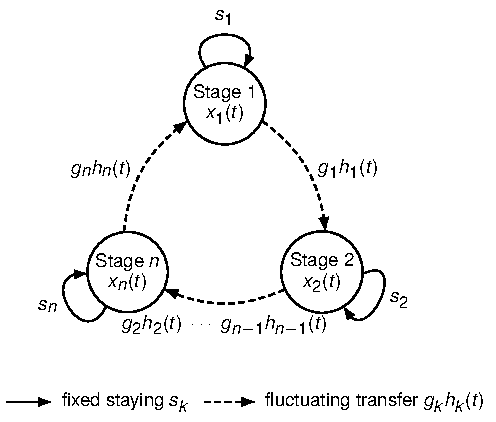
\includegraphics[width=84mm]{figures/intro-1.pdf}
\caption{Schematic of the discrete-time $n$-stage parasite life-cycle ring in~\eqref{eq:model-ring} (shown with stages $1$, $2$, and $n$ returning to stage $1$). Circular nodes represent sequential parasite stages with abundances $x_k(t)$, solid self-loops indicate fixed staying contributions $s_k \ge 0$, and dashed directed arcs indicate host-driven transfer contributions $g_k h_k(t)$ (fixing $h_k(t) \equiv 1$ gives a steady transfer)}\label{fig:intro-1}
\end{figure}

When $\E[h_k(t)] = 1$, the mean matrix $\mathbf{A}_0 = \E[\mathbf{A}(t)]$ is assumed primitive ($n = 1$, or $n \ge 2$ with at least one $s_k > 0$), with Perron root $\lambda = \spr(\mathbf{A}_0) > 0$ and positive right and left eigenvectors $\mathbf{v}$ and $\mathbf{w}$ normalized by $\mathbf{1}^{\mathsf{T}}\mathbf{v} = 1$ and $\mathbf{w}^{\mathsf{T}}\mathbf{v} = 1$. Where parallel host routes or staying and transfer terms share a matrix entry, we resolve them as finitely many labeled contributions $e$ from $j_e$ to $i_e$ with baseline weight $a_e > 0$ and fixed part $\mathbf{A}_{\mathrm{fixed}} \ge \mathbf{0}$,
\begin{equation}\label{eq:model-edges}
\mathbf{A}(t) = \mathbf{A}_{\mathrm{fixed}} + \sum_e a_e h_e(t)\mathbf{e}_{i_e}\mathbf{e}_{j_e}^{\mathsf{T}}, \qquad \mathbf{A}_0 = \mathbf{A}_{\mathrm{fixed}} + \sum_e a_e \mathbf{e}_{i_e}\mathbf{e}_{j_e}^{\mathsf{T}},
\end{equation}
where $\mathbf{e}_i$ is the $i$th unit vector. Following a line of descent forward weighted by reproductive value defines an irreducible, aperiodic reference Markov chain $P(j \to i) = w_i (\mathbf{A}_0)_{ij}/(\lambda w_j)$ with stationary law $\pi_k = w_k v_k$ \citep{bienvenu2015,bienvenu2017}. In~\eqref{eq:model-ring}, a reference lineage stays in stage $k$ with probability $m_k = s_k/\lambda$, giving geometric stays on $\{1, 2, \dots\}$ of mean $\tau_k = (1 - s_k/\lambda)^{-1} \ge 1$ (the lineage stay), circuit time $L$ of mean $\mathcal{T} = \sum_{k=1}^n \tau_k$ (the lineage generation time) and variance $\sum_{k=1}^n \tau_k(\tau_k - 1)$, and $\pi_k = \tau_k/\mathcal{T}$. At $\lambda = 1$ ($0 \le s_k < 1$), $\tau_k$ equals the ordinary mean stay $\tau_{k,0} = (1 - s_k)^{-1}$ and $\mathcal{T}$ equals $\mathcal{T}_0 = \sum_{k=1}^n \tau_{k,0}$. In continuous time, the gain-only ring is
\begin{equation}\label{eq:model-ct}
\frac{\mathrm{d}x_{k+1}}{\mathrm{d}t} = b_k \nu_k h_k(t) x_k(t) - (\nu_{k+1} + \mu_{k+1})x_{k+1}(t),
\end{equation}
with transfer exit rate $\nu_k > 0$, death rate $\mu_k \ge 0$, yield $b_k > 0$, mean-environment growth rate $r_0$, lineage exit rates $a_k = r_0 + \nu_k + \mu_k$, and generation time $T = \sum_{k=1}^n a_k^{-1}$.

\subsection{Host fluctuations}\label{sec:model-hosts}

In the baseline stochastic ring, hosts vary via stationary mean-one lognormal multipliers driven by first-order autoregressive (AR(1)) Gaussian processes,
\begin{equation}\label{eq:model-ar1}
h_k(t) = \exp\!\left(\sigma_k \xi_k(t) - \frac{\sigma_k^2}{2}\right), \qquad \xi_k(t+1) = \phi_k \xi_k(t) + \sqrt{1 - \phi_k^2}\,\epsilon_k(t+1),
\end{equation}
with independent innovations $\epsilon_k(t) \sim \mathcal{N}(0, 1)$, stationary $\xi_k(0) \sim \mathcal{N}(0, 1)$, log-abundance standard deviation (SD) $\sigma_k \ge 0$ (log variance $\sigma_k^2$, raw variance $\ee^{\sigma_k^2} - 1$), and lag-one log autocorrelation $\phi_k \in (-1, 1)$, giving $\E[h_k(t)] = 1$ and $\Cov(\xi_k(t), \xi_k(t-\ell)) = \phi_k^{|\ell|}$ (Fig.~\ref{fig:intro-2}). Positive geometric-memory comparisons take $0 \le \phi_k < 1$ with memory scale $\theta_k = \phi_k/(1 - \phi_k)$. Hosts are independent and unaffected by the parasite in the basic ring, whereas shared drivers $\delta(e)$ and real sensitivities $\kappa_e$ on edge $e$ use $h_e(t) = \exp(\sigma \kappa_e \xi_{\delta(e)}(t) - \sigma^2 \kappa_e^2/2)$ to preserve $\E[h_e(t)] = 1$.

\begin{figure}[htbp]
\centering
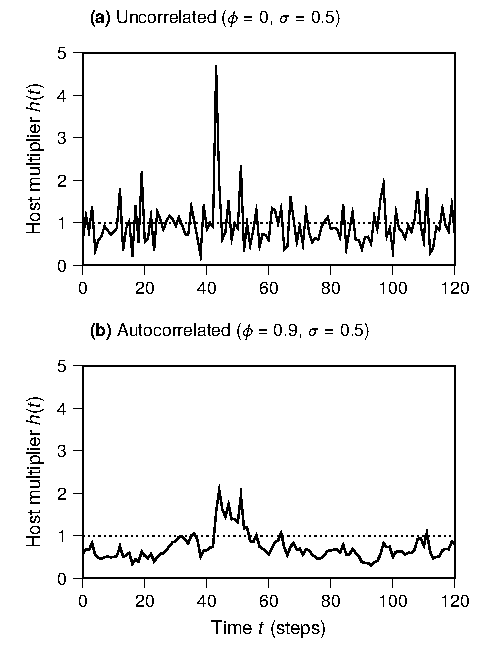
\includegraphics[width=84mm]{figures/intro-2.pdf}
\caption{Illustrative realizations of the mean-one lognormal host multiplier $h(t)$ in~\eqref{eq:model-ar1} over 120 steps with $\sigma = 0.5$ for (a) an uncorrelated host ($\phi = 0$) and (b) an autocorrelated host ($\phi = 0.9$). Solid curves use the same standard-Gaussian innovations and stationary start (seed 20261114), and horizontal dotted lines mark $\E[h(t)] = 1$ (synthetic model illustrations, not empirical host series)}\label{fig:intro-2}
\end{figure}

Four further environmental laws enter later sections. Sections~\ref{sec:ring} and~\ref{sec:mech} use jointly stationary centered unit-variance Gaussian linear processes $\xi_\delta(t) = \sum_{j=0}^{\infty} \psi_{\delta,j}\epsilon_\delta(t-j)$ with $\sum_{j=0}^{\infty} \psi_{\delta,j}^2 = 1$ and $\Psi_\delta = \sum_{j=0}^{\infty}|\psi_{\delta,j}| < \infty$ (covering damped second-order autoregressive (AR(2)) quasi-cycles and two-host Gaussian vector autoregressions). Continuous-time models in Section~\ref{sec:ring} use unit-variance Ornstein--Uhlenbeck (OU) log drivers $z_k(t)$ with covariance $\exp(-\alpha_k |t|)$ ($\alpha_k > 0$). Bounded-probability contact, thermal, and outage studies in Sections~\ref{sec:mech} and~\ref{sec:num} use two-state Markov multipliers $h(t) = 1 + \sigma\xi(t)$ ($\xi(t) \in \{-1, 1\}$), skewed two-state or on/off hosts, and periodic schedules of period $P$. Finally, Section~\ref{sec:exact} uses \citet{roerdink1988}'s two-stage ring $x_0(t+1) = g_1 x_1(t)$, $x_1(t+1) = s x_1(t) + g_0 h_t x_0(t)$ ($0 < s < 1$, $c = g_0 g_1 > 0$) with independent $h_t \sim \operatorname{Gamma}(p, 1/p)$ ($p > 0$, mean $1$, variance $1/p$).

\subsection{Reproduction number, baseline and loss}\label{sec:model-r0}

When $h_k(t) \equiv 1$, $g_k > 0$, and $0 \le s_k < 1$, designating $1 \le m \le n$ transfers as births splits $\mathbf{A}_0 = \mathbf{F} + \mathbf{V}$ ($\mathbf{F}$ holding the $m$ birth transfers and $\mathbf{V}$ the rest). The following proposition (proved below and refereed) links the whole-circuit number $R_0$, the next-generation number $R_{\mathrm{NG}}$, and $\lambda$.

\begin{proposition}[Birth convention and deterministic threshold]\label{prop:model-birth}
For the deterministic ring with $g_k > 0$, $0 \le s_k < 1$, and $1 \le m \le n$ designated birth transfers,
\begin{equation}\label{eq:model-r0}
R_0 = \prod_{k=1}^n \frac{g_k}{1 - s_k}, \qquad R_{\mathrm{NG}} = \spr\!\bigl(\mathbf{F}(\mathbf{I} - \mathbf{V})^{-1}\bigr) = R_0^{1/m}, \qquad \prod_{k=1}^n (\lambda - s_k) = \prod_{k=1}^n g_k,
\end{equation}
where $\mathbf{I}$ is the identity matrix. Counting every transfer gives $R_{\mathrm{NG}} = R_0^{1/n}$, the threshold is $R_0 = 1$ for every $m$, and $\ln\lambda = (\ln R_0)/\mathcal{T}_0 + O((\ln R_0)^2)$ as $\ln R_0 \to 0$ at fixed $s_k$ (exact at all $R_0$ when $n = 1$ and $s_1 = 0$).
\end{proposition}

\begin{proof}
Dividing the $m$ birth transfers by $R > 0$ gives $\prod_{k=1}^n (\lambda - s_k) = R^{-m}\prod_{k=1}^n g_k$. Setting $\lambda = 1$ yields $R^m = R_0$, so $R_{\mathrm{NG}} = R_0^{1/m}$ and $R_{\mathrm{NG}} = 1 \iff R_0 = 1$. Differentiating $\sum_{k=1}^n \ln[(\lambda - s_k)/(1 - s_k)] = \ln R_0$ with respect to $\ln\lambda$ at $\lambda = 1$ gives $\mathcal{T}_0 > 0$, yielding $\ln\lambda = (\ln R_0)/\mathcal{T}_0 + O((\ln R_0)^2)$ (exact when $n = 1, s_1 = 0$).
\end{proof}

Our default baseline fixes every rate at its arithmetic mean ($\E[h_e(t)] = 1$, giving $\mathbf{A}_0$). Alternative baselines fix lognormal hosts at their geometric mean (Section~\ref{sec:bounds}), host abundance at $\overline{H}$ inside an encounter curve $F(H)$ (Section~\ref{sec:mech}), or temperature at $\overline{T}$ inside thermal rates (Section~\ref{sec:mech}), and can reverse an effect's sign.

For a fixed nonzero nonnegative initial vector $\mathbf{x}(0)$ independent of future environments under stationary ergodic forcing with integrable logarithms, write $r = \lim_{t\to\infty} t^{-1}\ln\|\mathbf{x}(t)\|$. Adopting the zero-growth birth-divisor characterization of \citet{bacaer2013}, let $R_0^*$ be the common positive divisor on the $m$ birth transfers giving $r = 0$, and define
\begin{equation}\label{eq:model-loss}
\mathrm{cost} = \ln\lambda - r, \qquad D = \ln R_0 - m\ln R_0^*, \qquad \ln R_0^* = \frac{\ln R_0 - D}{m}.
\end{equation}
We write $C$ (or $C''$) for the $\sigma^2$ coefficient of $\mathrm{cost}$ and $\Gamma = \mathcal{T} C \sigma^2$ (summed over independent hosts) for the second-order term of the per-generation loss $\mathcal{T}(\ln\lambda - r)$. Non-ring networks use $\Delta$, the log restoring birth multiplier relative to threshold ($D = m\Delta$ in a ring). Negative losses are called gains, and neither $D$ nor $\Gamma$ is an integer-population extinction probability. The next proposition (proved below and refereed) establishes existence and invariance of $D$ in the lognormal AR(1) ring.

\begin{proposition}[Existence and invariance of the ring threshold loss]\label{prop:model-loss}
In~\eqref{eq:model-ring} with fixed $0 \le s_k < 1$ ($n = 1$, or $n \ge 2$ with some $s_k > 0$), $g_k > 0$, $1 \le m \le n$ birth transfers, and stationary AR(1) lognormal multipliers~\eqref{eq:model-ar1} with $|\phi_k| < 1$, $R_0^*$ exists uniquely and $D$ depends only on $(s_1, \dots, s_n)$ and the multiplier law, not on $(g_1, \dots, g_n)$ or $m$.
\end{proposition}

\begin{proof}
Rescaling $x_k \mapsto d_k x_k$ ($d_k > 0$) replaces $g_k$ by $g_k d_{k+1}/d_k$ without changing $s_k$, $h_k(t)$, or $r$, so $r$ depends only on $y = \ln\prod_{k=1}^n g_k$, written $r(y)$. Dividing $m$ births by $R$ shifts $y$ to $y - m\ln R$, so at a unique root $r(y_0) = 0$ we have $D = y_0 - \sum_{k=1}^n \ln(1 - s_k)$, independent of $g_k$ and $m$. If $n = 1$ and $s_1 = 0$, $r(y) = y - \sigma_1^2/2$ gives unique $y_0 = \sigma_1^2/2$. Otherwise some $s_k > 0$. Setting $g_k = c_k \ee^{y/n}$ ($\prod_{k=1}^n c_k = 1$), each path of length $t$ with $j$ transfers carries $\ee^{j y/n}$ times a positive weight, making $\ln\|\mathbf{x}(t)\|$ and hence $r(y)$ convex and nondecreasing. Integrable lognormal norms and the never-transferring path give $\max_k \ln s_k \le r(y) < \infty$, so $r(y)$ is finite and continuous. Since $r(y) \le \E[\ln\max_k(s_k + c_k \ee^{y/n} h_k(0))] \to \max_k \ln s_k < 0$ as $y \to -\infty$ and the always-transferring path gives $r(y) \ge y/n + c_0 \to +\infty$ as $y \to +\infty$ (finite $c_0$), a root exists, and convexity with a negative left limit rules out two roots.
\end{proof}

Along a fixed noise direction in this ring, Section~\ref{sec:ring} proves $D = \Gamma_0 + O(\sigma^4)$, where $\Gamma_0$ evaluates $\Gamma$ at $\tau_{k,0} = (1 - s_k)^{-1}$ ($\Gamma \ne \Gamma_0$ in general away from threshold).

\subsection{Hosts with their own dynamics}\label{sec:model-dyn}

When an established parasite affects host prevalence or survival (Section~\ref{sec:dyn}), we model a continuous-time ring of $n$ blocks coupled solely through scalar infection pressure ($u_k$ entering block $k$, $v_k = u_{k+1}$ leaving it). Around a positive equilibrium, local stability requires all linearized eigenvalues to have negative real part and is governed by each block's relative linear frequency response $E_k(z) = N_k(z)/D_k(z)$ (derived independently twice, checked numerically by a third party, and refereed). The first three blocks are an unregulated stage ($\mathrm{L}$, $\dot{w} = u - a w$, $v = c w$, $E_{\mathrm{L}} = a/(z + a)$), a regulated transfer ($\mathrm{R}$, $v = c f(w) w$, $\kappa = -w^* f'(w^*)/f(w^*)$, $E_{\mathrm{R}} = (1 - \kappa)a/(z + a)$), and a constant-size host ($\mathrm{S}$, $\dot{I} = u(N - I) - a I$, $v = c I$, prevalence $p = I^*/N \in (0, 1)$, $E_{\mathrm{S}} = a/[z + a/(1 - p)]$). The two dynamic-host blocks are a susceptible--infected host killed at rate $\alpha > 0$ ($\mathrm{V}$, $\dot{N} = \Phi(N) - \alpha I$, $\dot{I} = u(N - I) - a I$, $v = c I$, requiring $a \ge \alpha$, with $\rho = -\Phi'(N^*)$, $q = a$, $d = a/(1 - p)$, $h = \alpha p$) and a macroparasite host after \citet{anderson1978} ($\mathrm{M}$, $\dot{H} = \Phi(H) - \alpha P$, $\dot{P} = u H - \xi P - \alpha \varepsilon P^2/H$, $v = \lambda_P P$, $\varepsilon \ge 1$, mean burden $m = P^*/H^*$, $\rho = -\Phi'(H^*)$, $h = \alpha m$, $q = \xi + \varepsilon h$, $d = \xi + 2\varepsilon h$). Blocks $\mathrm{V}$ and $\mathrm{M}$ and the cycle characteristic polynomial satisfy
\begin{equation}\label{eq:model-blocks}
E_{\mathrm{V,M}}(z) = \frac{q(z + \rho)}{(z + \rho)(z + d) + d h}, \qquad \chi(z) = \prod_{k=1}^n D_k(z) - \prod_{k=1}^n N_k(z),
\end{equation}
retaining internal modes that can cancel in $\prod_{k=1}^n E_k(z) = 1$.

\begin{table}[t]
\caption{Summary of principal notation, meanings, and units}\label{tab:model-notation}
{\scriptsize\setlength{\tabcolsep}{0.5pt}
\begin{tabular*}{\textwidth}{@{\extracolsep{\fill}}llll@{}}
\toprule
Symbol & Meaning & Units & First use \\
\midrule
$x_k, \mathbf{x};\, X_k$ & Stage amount, vector; local population variable & Population & \eqref{eq:model-ring}, \S\ref{sec:dyn} \\
$n, k$ & Number of stages in ring; stage index (mod $n$) & Dimless & \eqref{eq:model-ring} \\
$s_k, g_k$ & Staying and transfer multipliers per census step & Dimless & \eqref{eq:model-ring} \\
$h_k(t), \xi_k(t)$ & Mean-one host multiplier; standardized log driver & Dimless & \eqref{eq:model-ring}, \eqref{eq:model-ar1} \\
$\sigma_k, \phi_k$ & Log-host SD and lag-1 correlation & Dimless & \eqref{eq:model-ar1} \\
$\theta_k$ & Memory scale $\phi_k/(1-\phi_k)$ & Steps & \S\ref{sec:model-hosts} \\
$\kappa_e$ & Signed noise sensitivity on labeled edge $e$ & Dimless & \S\ref{sec:model-hosts} \\
$p$ & Gamma shape in \S\ref{sec:exact}; prevalence in \S\ref{sec:dyn} & Dimless & \S\ref{sec:model-hosts}, \S\ref{sec:model-dyn} \\
$\nu_k, \mu_k, \alpha_k$ & Continuous transfer exit, death, and OU rates & Time$^{-1}$ & \eqref{eq:model-ct}, \S\ref{sec:model-hosts} \\
$b_k$ & Baseline descendants per transfer or leaver & Event$^{-1}$ & \eqref{eq:model-ct}, \S\ref{sec:num} \\
$u, v, E(z)$ & Block infection input, output, frequency response & Block, dimless & \S\ref{sec:model-dyn} \\
$\rho = -\Phi'$ & Negative slope of host total net production & Time$^{-1}$ & \S\ref{sec:model-dyn} \\
$\alpha, \varepsilon$ & Infection host death rate; burden clumping & Time$^{-1}$, dimless & \S\ref{sec:model-dyn} \\
$c, \mu$ & Contact and waiting-death probabilities per step & Dimless & \S\ref{sec:mech} \\
$T_t, \sigma_T$ & Daily temperature and temperature SD & $^{\circ}\mathrm{C}$ & \S\ref{sec:mech} \\
$\widehat{K}(z), K(\ell)$ & Sheltered kernel transform and lag-$\ell$ mass & Descendants & \S\ref{sec:model-ring}, \S\ref{sec:mech} \\
$\mathbf{A}_0, \lambda, \mathbf{v}, \mathbf{w}$ & Mean matrix, Perron root, right/left eigenvectors & Map, vectors & \eqref{eq:model-edges} \\
$r, r_0$ & Stochastic and mean-environment log growth rates & Rate & \eqref{eq:model-ct}, \eqref{eq:model-loss} \\
$\tau_k, \mathcal{T}, \mathcal{T}_0$ & Lineage stay, lineage and threshold gen.\ times & Steps & \S\ref{sec:model-ring} \\
$R_0, R_{\mathrm{NG}}, R_0^*$ & Circuit $R_0$, $m$-birth $R_0$, stochastic divisor & Dimless & \eqref{eq:model-r0}, \eqref{eq:model-loss} \\
$\mathrm{cost}, \Gamma, D, \Delta$ & Step loss, $\sigma^2$ gen.\ loss, $\ln R_0$ loss, shift & Log units & \eqref{eq:model-loss} \\
$J, J_2$ & Thermal curvature shift or lineage log-penalty rate & Log units & \S\ref{sec:model-methods}, \S\ref{sec:mech} \\
$\mathbf{B}_e, c_e, \mathbf{Q}, \mathbf{T}_\perp$ & Edge matrix, edge frequency, projection, transverse & Dimless & \eqref{eq:model-c2} \\
$C, C''$ & Second-order per-step growth-cost coefficients & Step$^{-1}\sigma^{-2}$ & \eqref{eq:model-c2} \\
$\rho_{\delta\delta'}(\ell)$ & Directed lag-$\ell$ covariance $\E[\xi_\delta(t)\xi_{\delta'}(t-\ell)]$ & Dimless & \eqref{eq:model-c2} \\
$V_2$ & Unscaled within-environment lineage variance rate & Step$^{-1}$ & \S\ref{sec:model-methods}, \S\ref{sec:bounds} \\
$P$ & Environmental period (distinct from burden $P$) & Steps & \S\ref{sec:model-hosts} \\
\bottomrule
\end{tabular*}}
\end{table}

\subsection{Methods of derivation and checking}\label{sec:model-methods}

On~\eqref{eq:model-edges} with primitive $\mathbf{A}_0$ and $h_e(t) = \exp(\sigma \kappa_e \xi_{\delta(e)}(t) - \sigma^2 \kappa_e^2/2)$, set $\mathbf{M} = \mathbf{A}_0/\lambda$, $\mathbf{Q} = \mathbf{I} - \mathbf{v}\mathbf{w}^{\mathsf{T}}$, $\mathbf{T}_\perp = \mathbf{M} - \mathbf{v}\mathbf{w}^{\mathsf{T}}$, $\mathbf{B}_e = (a_e/\lambda)\mathbf{e}_{i_e}\mathbf{e}_{j_e}^{\mathsf{T}}$, $c_e = \mathbf{w}^{\mathsf{T}}\mathbf{B}_e\mathbf{v}$, and $\rho_{\delta\delta'}(\ell) = \E[\xi_\delta(t)\xi_{\delta'}(t-\ell)]$. The published second-order coefficient \citep{ruelle1979,tuljapurkar1982a,tuljapurkar2006} and discrete-time lognormal remainder bound (proved and refereed for Gaussian linear processes with $\Psi_\delta < \infty$ in Section~\ref{sec:ring} and Appendix~A, with uniform AR(1) constants on compact families via Lemma~U and separate $O(|\sigma|^3)$ or symmetric $O(\sigma^4)$ bounded-driver remainders) are
\begin{align}
C'' &= \sum_{e,e'} \kappa_e \kappa_{e'}\biggl[\frac{c_e c_{e'}}{2}\rho_{\delta(e)\delta(e')}(0) \nonumber\\
&\qquad\qquad - \sum_{j=0}^{\infty} \rho_{\delta(e)\delta(e')}(j+1)\,\mathbf{w}^{\mathsf{T}}\mathbf{B}_e \mathbf{T}_\perp^j \mathbf{Q}\mathbf{B}_{e'}\mathbf{v}\biggr], \label{eq:model-c2}\\
\bigl|\ln\lambda - r(\sigma) - C''\sigma^2\bigr| &\le K\sigma^4 \qquad (|\sigma| \le \sigma_0). \label{eq:model-rem}
\end{align}
Constants $K$ and $\sigma_0$ are non-explicit, and continuous-time or thermal expansions give formal coefficients only. Strict coefficient inequalities transfer to small $|\sigma|$ where~\eqref{eq:model-rem} holds, whereas equal coefficients do not settle finite-noise order. Section~\ref{sec:bounds} uses path expansions on $P$ with reward $S_T = \sum_{t=1}^T \ln h_{e_t}(t)$ to prove $r - \ln\lambda \ge -\sum_e c_e \ell_e$ ($\ell_e = -\E[\ln h_e]$) and rewrite $C''\sigma^2 = \sigma^2(J_2 - \tfrac{1}{2}V_2)$ via $J_2 = \tfrac{1}{2}\sum_e c_e \kappa_e^2$ and within-environment lineage reward variance rate $\sigma^2 V_2$. Exact checks use periodic monodromy products $\boldsymbol{\mathcal{F}} = \mathbf{A}(P-1)\cdots\mathbf{A}(0)$ ($r_P = P^{-1}\ln\spr(\boldsymbol{\mathcal{F}})$; \citealp{bacaer2007}) and \citet{roerdink1988}'s Kummer density and Tricomi $U(p, b, \kappa)$ growth formula (Section~\ref{sec:exact}).

Simulations followed written protocols with tolerances fixed beforehand. Core ring and coupled-host equations had independent derivations, second-party code reproductions, and referee checks. The Cary Institute and National Ecological Observatory Network (NEON) analyses were computed once. Lean~4 checked the statements and components listed in the reconciled coverage inventory archived with the Lean sources (see Code availability). Some model identifications, stochastic limits and remainder estimates remain outside that coverage and rely on written proofs. Numerical settings and validation logs are given in Online Resource~1.

\subsection{Use of large language models}\label{sec:model-llm}

{\sloppy
All derivations, proofs, simulation and verification scripts, literature searches and reading cards, referee reports, Lean~4 formalizations, and manuscript text were produced by large language model systems (Claude, Anthropic; Codex, OpenAI; and a Gemini-based agent run through Cursor, here called Carbon). Separate model instances derived core results without access to each other's intermediate work. Second-party scripts reproduced closed forms and simulations from specifications, followed by referee audits and Lean checks (Section~\ref{sec:model-methods}; details in Online Resource~1). These checks do not replace human accountability or specialist review. No person is recorded as having checked a derivation, simulation, literature card, or formal proof file. The author reviewed the worked example and the verification records and approved the manuscript.\par}

\FloatBarrier
\section{A worked example: one, two and three hosts}\label{sec:example}

Before turning to the general derivations, we compare life cycles with one, two, and three hosts in the linear, rare-parasite ring model of Section~\ref{sec:model} (Eq.~\eqref{eq:model-ring}). All parameter values here are illustrative choices in that model rather than measurements on a specific species. Take one month as the time step (results hold in units of the step). Each mean model is calibrated to $R_0 = \lambda = 1$ (the invasion threshold without fluctuations, where $R_0$ is the baseline expected descendants completing one cycle and $\lambda$ is the mean-matrix per-step growth factor), with memoryless geometric stage stays of mean $\tau_k$ months, staying fractions $1 - 1/\tau_k$, mean transfers $1/\tau_k$, and mean generation time $\mathcal{T} = \sum_{k=1}^n \tau_k$ across the $n$ stages. The parasite spends a mean stay of $a = 6$ months in the one stage whose outward transfer depends on a fluctuating host, while every other host is a steady stage (constant host multiplier $h_k(t) \equiv 1$). That host's abundance, scaled to an arithmetic mean of one, has a logarithm that follows a Gaussian first-order autoregressive process with standard deviation $\sigma$ (variance $\sigma^2$) and monthly lag-one correlation $\phi$ (Eq.~\eqref{eq:model-ar1}). Writing $\theta = \phi/(1 - \phi)$ for the host memory scale (in months), we compare uncorrelated monthly host numbers ($\phi = 0$, $\theta = 0$) with multi-month booms and busts ($\phi = 0.8$, $\theta = 4$ months).

Here $\Gamma$ (Proposition~\ref{prop:ring-gamma}, Eq.~\eqref{eq:ring-gamma}) is the quadratic (second-order, meaning the leading effect of small fluctuations, proportional to $\sigma^2$) approximation to the threshold loss $D$ in $\ln R_0$ (Eq.~\eqref{eq:model-loss}, Proposition~\ref{prop:bounds-r0star}). A rare parasite invades only if $\ln R_0$ exceeds $D$, so a relative loss of $2$ means fluctuations raise the invasion hurdle twice as much as in the one-host cycle of stay $a = 6$ months, where $\Gamma/\sigma^2 = 1/(2a) = 1/12 \approx 0.08333$ at every $\phi$ (Proposition~\ref{prop:ring-band}).

\begin{table}[htbp]
\caption{Fluctuation loss across illustrative one-, two-, and three-host life cycles in series and across alternative hosts in parallel$^{\mathrm{a,b}}$}\label{tab:example}
{\footnotesize\setlength{\tabcolsep}{4pt}
\begin{tabular*}{\textwidth}{@{\extracolsep{\fill}}lrrrrr@{}}
\toprule
\multicolumn{6}{@{}l@{}}{\textit{Part A. Obligate hosts in series (fluctuating stay $a = 6$ months)}} \\
\addlinespace[2pt]
 & & \multicolumn{2}{c}{Autocorrelated ($\phi = 0.8$)} & \multicolumn{2}{c}{Uncorrelated ($\phi = 0$)} \\
\cmidrule(lr){3-4}\cmidrule(lr){5-6}
Life cycle & $\mathcal{T}$ (mo) & $\Gamma/\sigma^2$ & Relative & $\Gamma/\sigma^2$ & Relative \\
\midrule
1 host (no steady stage) & $6$ & $0.08333$ & $1.00$ & $0.08333$ & $1.00$ \\
2 hosts, steady stay $3$ & $9$ & $0.20370$ & $2.44$ & $0.05556$ & $0.67$ \\
2 hosts, steady stay $60$ & $66$ & $0.04254$ & $0.51$ & $0.00758$ & $0.091$ \\
3 hosts, steady stays $30 + 30$ & $66$ & $0.06261$ & $0.75$ & $0.00758$ & $0.091$ \\
3 hosts, steady stays $1 + 59$ & $66$ & $0.04744$ & $0.57$ & $0.00758$ & $0.091$ \\
\bottomrule
\end{tabular*}
\par\vspace{3pt}
\begin{tabular*}{\textwidth}{@{\extracolsep{\fill}}lrr@{}}
\toprule
\multicolumn{3}{@{}l@{}}{\textit{Part B. Equal-share matched alternative hosts in parallel (stays $6$ and $24$ months, $\mathcal{T} = 30$)}} \\
\addlinespace[2pt]
Alternative hosts $M$ & Relative loss, independent ($\rho = 0$) & Relative loss, perfectly synchronous ($\rho = 1$) \\
\midrule
$1$ & $1.00$ & $1.00$ \\
$2$ & $0.50$ & $1.00$ \\
$3$ & $0.33$ & $1.00$ \\
$4$ & $0.25$ & $1.00$ \\
$5$ & $0.20$ & $1.00$ \\
\bottomrule
\end{tabular*}}
\par\smallskip\noindent\parbox{\textwidth}{\scriptsize\raggedright
$^{\mathrm{a}}$Each mean model is calibrated to $R_0 = \lambda = 1$. Part~A divides $\Gamma/\sigma^2$ by the one-host reference $\Gamma(6)/\sigma^2 = 1/12 \approx 0.08333$. Part~B replaces the fluctuating transfer at fixed mean total transfer by the equal-share average of $M$ hosts with matched log variance and memory at $\phi = 0.8$ ($M = 1$ reference $\Gamma/\sigma^2 = 0.08939$, with cross-covariances at every lag equal to $\rho$ times the common autocovariance), and the same ratios $1/M$ and $1.00$ hold at $\phi = 0$ ($M = 1$ reference $\Gamma/\sigma^2 = 0.01667$).\\[2pt]
$^{\mathrm{b}}$Direct simulation of the exact threshold loss $D$ (Eq.~\eqref{eq:model-loss}) at $\sigma = 0.3$ ($600$ replicates, at least $20{,}000$ months each) covered $18$ cases: $1$ host, $2$ hosts with steady stays $3$ and $60$, $3$ hosts with steady stays $30 + 30$ and $1 + 59$, parallel $M = 1, 2, 3$ independent ($\rho = 0$), and parallel $M = 3$ synchronous ($\rho = 1$), each at $\phi = 0$ and $\phi = 0.8$. Simulated $D$ gave values slightly above the quadratic predictions (by $0.0001$--$0.0008$, largest standard error $0.00027$) and ranked the cases as the formulas do, with formula ties reproduced within simulation error.\par}
\end{table}

\begin{figure}[htbp]
\centering
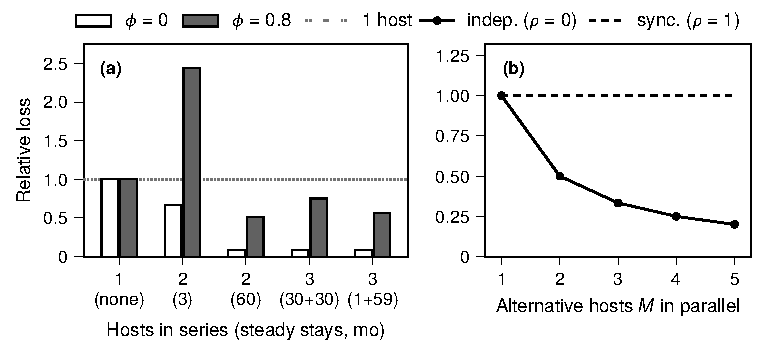
\includegraphics[width=129mm]{figures/example-1.pdf}
\caption{Relative second-order fluctuation loss across illustrative life cycles (parameters as in Table~\ref{tab:example}). Panel~(a) compares one, two, and three obligate hosts in series with a $6$-month fluctuating stay and the indicated steady stays (in months) under uncorrelated ($\phi = 0$, open bars) and autocorrelated ($\phi = 0.8$, shaded bars) host abundance, relative to one host (gray dotted line at $1.0$, $\Gamma/\sigma^2 = 1/12$). Panel~(b) compares $M = 1$ to $5$ equal-share matched alternative hosts in parallel at fixed mean total transfer in a $(6, 24)$-month cycle at $\phi = 0.8$ when cross-host correlation $\rho$ (under Proposition~\ref{prop:ring-alt}) is independent ($\rho = 0$, solid curve with markers) or perfectly synchronous ($\rho = 1$, black dashed line)}\label{fig:example-1}
\end{figure}

First, the number of obligate hosts in series does not decide the outcome. With two hosts in sequence at $\phi = 0.8$, adding a $3$-month steady stay raises the fluctuation loss to $2.44$ times the one-host value, whereas a $60$-month steady stay lowers it to $0.51$ (Table~\ref{tab:example}, Part~A, Fig.~\ref{fig:example-1}a). Time spent in the sheltered stage, rather than host count, governs whether a second host amplifies or halves the penalty (Proposition~\ref{prop:ring-steady}(c), Eq.~\eqref{eq:ring-steady}).

Second, without host memory ($\phi = 0$), only total time outside the fluctuating transfer matters. The second-order loss reduces to $\Gamma = \sigma^2/(2\mathcal{T})$ (Propositions~\ref{prop:ring-band} and~\ref{prop:ring-steady}(b)), so the two-host cycle with a $60$-month steady stay and both three-host cycles ($30 + 30$ and $1 + 59$ months) share $\mathcal{T} = 66$ months and the same relative loss of $0.091$ ($\Gamma/\sigma^2 = 0.00758$). For independent gamma hosts, a one-step exposed stage, and a geometric steady stay, exact threshold loss likewise decreases strictly with steady-stay duration at every fixed positive variance, although that exact benchmark does not cover the $6$-month exposed stage used here (Section~\ref{sec:exact}, Theorem~\ref{thm:exact-mono}).

Third, when host fluctuations carry memory ($\phi > 0$), how sheltered time is divided across stages changes the loss, whereas compartment labels alone do not. At $\phi = 0.8$ and $\mathcal{T} = 66$ months, splitting $60$ sheltered months into $30 + 30$ raises the relative loss from $0.51$ to $0.75$, whereas $1 + 59$ gives $0.57$ (Table~\ref{tab:example}, Part~A, Fig.~\ref{fig:example-1}a). Dividing a sheltered stay into equal substages raises the loss under memory (Proposition~\ref{prop:mech-renewal}), and at fixed $n$ and $\mathcal{T}$ the loss lies between the values for $n - 1$ unit stays and for equal stays (Proposition~\ref{prop:ring-band}, Eq.~\eqref{eq:ring-gamma}). Here, relabeling the two unchanged steady compartments as one host or two leaves the matrix identical. More generally, equal complete sheltered kernels and unchanged exposed dynamics preserve growth and threshold (Section~\ref{sec:mech}, Lemma~\ref{lem:mech-kernel}).

Fourth, under multi-month boom-and-bust dynamics, a short sheltered stay can make things worse. For a two-stage cycle with fluctuating stay $a$ and steady stay $b$ (Proposition~\ref{prop:ring-steady}(c), Eq.~\eqref{eq:ring-steady}), adding $b$ raises $\Gamma$ above the one-host value whenever $a > 1$ and $b < a(2a - 1)\theta/(a + \theta)$ (Section~\ref{subsec:exact-memory}, Proposition~\ref{prop:exact-mem-ring}, Eq.~\eqref{eq:exact-mem-add}). At $a = 6$ and $\theta = 4$ months, $b = 26$ gives relative loss $1.01$ and $b = 27$ gives $0.98$, so a sheltered stay (a ``safe zone'') helps only once it exceeds this threshold (here $26.4$ months, more than six times the memory scale $\theta$).

Fifth, at fixed mean total transfer, equal shares of alternative hosts with matched log variance and memory used in parallel at the fluctuating step divide that step's second-order loss by their number when they fluctuate independently, whereas partial synchrony weakens this reduction, perfect synchrony gives no reduction, and a much noisier newcomer can raise the loss. Replacing one fluctuating host in a $(6, 24)$-month cycle by one to five such equal-share hosts ($M = 1$ to $5$) multiplies the loss by $[1 + \rho(M - 1)]/M$ when cross-covariances at every lag equal $\rho$ times the common autocovariance, giving $1/M$ ($0.50$ at $M = 2$ and $0.20$ at $M = 5$) at $\rho = 0$ and $1.00$ at $\rho = 1$ at both $\phi = 0.8$ and $\phi = 0$ (Table~\ref{tab:example}, Part~B, Fig.~\ref{fig:example-1}b, Proposition~\ref{prop:ring-alt}). In contrast, equal shares of independent hosts with variances $\sigma^2$ and $9\sigma^2$ and matched memory multiply the loss by $2.5$ (Proposition~\ref{prop:ring-alt}, with the general $\phi = 0$ newcomer inequality in Proposition~\ref{prop:mech-routes}, Eq.~\eqref{eq:mech-newcomer}).

Direct simulation of the exact threshold loss $D$ at $\sigma = 0.3$ (600 replicates, at least 20{,}000 months each) for the 18 cases listed in note~b gave values slightly above the quadratic predictions (by $0.0001$--$0.0008$, largest standard error $0.00027$) and ranked the cases as the formulas do, with formula ties reproduced within simulation error (Table~\ref{tab:example}, Eq.~\eqref{eq:model-loss}). The following sections prove these statements in general and show where they stop holding.

\section{Second-order theory of the ring}\label{sec:ring}

\paragraph{In brief.}
For a rare parasite, the second-order growth loss is the leading effect of small host fluctuations. When scarcity wastes failed transfers, stays are memoryless, and independent hosts have nonnegative memory, a sufficiently long steady stay reduces this loss at fixed existing stays. Obligate host count alone provides no protection. At fixed mean total transfer, independent alternative hosts with matched fluctuation laws reduce that transfer's contribution to the loss.

Host fluctuations affect a parasite through the times at which its descendants encounter each host. We analyze this sampling to second order in the gain-only ring of Section~\ref{sec:model}, with arithmetic-mean rates as baseline and $\sigma^2 > 0$ for strict comparisons. Write $C$ for the coefficient of per-step growth cost $\ln\lambda-r$ and $\Gamma = \mathcal{T} C \sigma^2$ for the loss per lineage generation. Proofs are in Appendix~\ref{app:ring}, and verification details are in Online Resource~1.

\subsection{Returns of a line of descent and the ring formula}\label{subsec:ring-formula}

The second-order cost can be written in terms of the time between successive uses of a transfer by a reference lineage (the renewal gap $L_e$, of mean $\mathcal{T}_e$; Proposition~\ref{prop:ring-lineage}, Appendix~\ref{app:ring}).

The ring is primitive when $n = 1$ or some $s_k > 0$. Stage $k$ has lineage staying probability $m_k = s_k / \lambda < 1$. Its geometric stay on $\{1, 2, \dots\}$ has mean $\tau_k = 1/(1 - m_k) \ge 1$, and $\mathcal{T} = \sum_{k=1}^n \tau_k$. One circuit separates successive uses of a transfer.

\begin{proposition}[One fluctuating transfer in a geometric ring]\label{prop:ring-gamma}
In a primitive $n$-stage gain-only ring with fixed stays $s_k \ge 0$, mean transfers $g_k > 0$, lineage stays $\tau_k = 1/(1 - s_k/\lambda)$, and generation time $\mathcal{T} = \sum_{k=1}^n \tau_k$, let one transfer carry $h(t) = \exp(z(t) - \sigma^2/2)$ with centered stationary Gaussian $\mathrm{AR}(1)$ driver $z(t)$ of variance $\sigma^2 > 0$ and autocorrelation $\phi^\ell$ ($0 \le \phi < 1$), while all other entries are fixed. Put $\theta = \phi/(1 - \phi)$ and $R = \prod_{k=1}^n (1 + \tau_k/\theta)^{-1}$ for $\phi > 0$ ($R = 0$ at $\phi = 0$). Then $C = (1 + 2\theta)/(2\mathcal{T}^2) - \mathcal{T}^{-1} R/(1 - R)$, and the second-order loss per generation is
\begin{equation}
\Gamma = \sigma^2 \left[ \frac{1 + 2\theta}{2\mathcal{T}} - \frac{R}{1 - R} \right].
\label{eq:ring-gamma}
\end{equation}
Neither which transfer fluctuates nor the cyclic order of stages changes $\Gamma$. Independent $\mathrm{AR}(1)$ hosts add their coefficients, and for each fixed primitive ring of this form $\ln\lambda - r = C\sigma^2 + O(\sigma^4)$ as $\sigma \to 0$ (Theorem~\ref{thm:ring-rem-ar1}).
\end{proposition}

Equation~\eqref{eq:ring-gamma} separates two opposing effects of positive host memory, namely integrated host variance $(1 + 2\theta)/(2\mathcal{T})$ and the return discount $R/(1 - R)$ across circuits.

\subsection{The band and comparisons across hosts in series}\label{subsec:ring-series}

Bounds on $R$ confine $\Gamma$ to a band.

\begin{proposition}[The band, memory limits, and unequal stays]\label{prop:ring-band}
Under Proposition~\ref{prop:ring-gamma} ($0 \le \phi < 1$, $\sigma^2 > 0$),
\begin{equation}
\frac{\sigma^2}{2\mathcal{T}} \le \Gamma \le \frac{\sigma^2(1 + 2\theta)}{2\mathcal{T}},
\label{eq:ring-band}
\end{equation}
with left equality if and only if $\phi = 0$ or $n = 1$, so $\phi > 0$ strictly raises $\Gamma$ when $n \ge 2$. As $\phi \to 0$, $C \to 1/(2\mathcal{T}^2)$. Taking $C$ first and then $\phi \uparrow 1$, $C \to (1 - \mathrm{CV}^2)/(2\mathcal{T})$, where $\mathrm{CV}^2 = \Var(L)/\mathcal{T}^2$ and $\Var(L) = \sum_{k=1}^n \tau_k(\tau_k - 1)$. At fixed $n$, $\mathcal{T}$, and $0 < \phi < 1$, equal stays maximize $\Gamma$ and setting $n - 1$ stays to $1$ minimizes it (all tie at $\phi = 0$).
\end{proposition}

Two stays long relative to $\theta$ can approach the upper edge. One long stay does not suffice (details in Online Resource~1).

The effect of sequential hosts depends on what is held fixed.

\begin{proposition}[Hosts in series]\label{prop:ring-series}
Let all $n$ transfers of a primitive gain-only ring follow independent Gaussian $\mathrm{AR}(1)$ hosts with variance $\sigma^2 > 0$ and memory $0 \le \phi < 1$. Put $\bar{\tau} = \mathcal{T}/n$ and $P = \prod_{k=1}^n (1 + \tau_k/\theta)$ for $\phi > 0$.
\begin{enumerate}
\item[(i)] At fixed $\bar{\tau}$, $\sigma^2/(2\bar{\tau}) \le \Gamma \le \sigma^2(1 + 2\theta)/(2\bar{\tau})$, with left equality if and only if $\phi = 0$ or $n = 1$; no ring beats one stage at $\bar{\tau}$, though $n$ does not order $n \ge 2$ (at $\phi = 0.9$, stays $(10, 10)$ give $0.371\sigma^2$ whereas $(1, 1, 28)$ give $0.214\sigma^2$).
\item[(ii)] For equal stays $\tau$ and $a = 1 + \tau/\theta$, $\Gamma_n = \sigma^2[(1 + 2\theta)/(2\tau) - n/(a^n - 1)]$ ($\phi > 0$), strictly increasing in $n$ at fixed $\tau$ and strictly decreasing in $\tau$ at fixed $n$ ($\sigma^2/(2\tau)$ at $\phi = 0$).
\item[(iii)] Keeping existing $\tau_k$ fixed and appending a stage of stay $\mathcal{T}/n$ on its own host changes $\Gamma$ by $\sigma^2[P(x - 1) + 1]/[(P - 1)\{P(1 + x/n) - 1\}]$ ($x = \mathcal{T}/\theta$), positive for $0 < \phi < 1$ and zero at $\phi = 0$ (fixing physical rates instead alters $\lambda$ and every $\tau_k$).
\item[(iv)] Multiplying every $\tau_k$ by $c > 1$ at fixed host laws strictly lowers $\Gamma$.
\item[(v)] At fixed equal rates ($\tau > 1$, $0 < \phi < 1$), the per-step coefficient $f_n = (1 + 2\theta)/(2n\tau^2) - [\tau(a^n - 1)]^{-1}$ has increments $f_{n+1} - f_n$ changing sign at most once, and some $f_n > f_1$ if and only if $\theta > \tau/[2(\tau - 1)]$.
\end{enumerate}
\end{proposition}

\subsection{A steady stage and alternative hosts}\label{subsec:ring-steady}

We test Dobson's storage (``parking lot'') argument \citep{dobson2020} by adding a steady stage at fixed existing geometric lineage stays and host laws.

\begin{proposition}[Adding a steady stage and the diffusion index]\label{prop:ring-steady}
For independent $\mathrm{AR}(1)$ hosts ($0 \le \phi_k < 1$) in a primitive geometric ring, put $S_I = \sum_{k=1}^n \sigma_k^2(1 + 2\theta_k)$, $S = \sum_{k=1}^n \sigma_k^2$, and second-order per-step growth-variance term $V = S_I / \mathcal{T}^2$.
\begin{enumerate}
\item[(a)] Adding stay $t$ with host variance $v$ and memory $\theta_v$ lowers $\mathcal{T}V = S_I / \mathcal{T}$ if and only if $v(1 + 2\theta_v)/t < S_I / \mathcal{T}$; a steady stage ($v = 0$) lowers $\mathcal{T}V$ whenever $S_I > 0$ (leaving zero unchanged).
\item[(b)] When all $\phi_k = 0$, $\Gamma = S/(2\mathcal{T})$ changes by $(v\mathcal{T} - St)/[2\mathcal{T}(\mathcal{T} + t)]$, negative if and only if $v/t < S/\mathcal{T}$.
\item[(c)] For one fluctuating host of stay $a \ge 1$ ($\sigma^2 > 0$, $0 \le \phi < 1$) and one steady stage of stay $b \ge 1$ (not both $1$), against $\Gamma(a)/\sigma^2 = 1/(2a)$ for one stage,
\begin{equation}
\frac{\Gamma(a,b)}{\sigma^2} = \frac{1 + 2\theta}{2(a + b)} - \frac{\theta^2}{\theta(a + b) + ab}, \qquad \lim_{b \to \infty} \frac{(a + b)\Gamma(a,b)}{\sigma^2} = \frac{1 + 2\theta}{2} - \frac{\theta^2}{\theta + a},
\label{eq:ring-steady}
\end{equation}
so $\Gamma(a,b) \to 0$ as $b \to \infty$ at fixed $a, \theta$ (taking $\sigma \to 0$ before $b \to \infty$).
\item[(d)] With one fluctuating host ($\sigma^2 > 0$, $0 \le \phi < 1$), put $k = 2\Gamma/(\mathcal{T}V) \in [1/(1 + 2\theta), 1]$, $L = \ln R_0 / \sigma^2$, and $E = 2(\ln R_0 - \Gamma)/(\mathcal{T}V) = 2\mathcal{T}\ln R_0 / [\sigma^2(1 + 2\theta)] - k$. In a Brownian diffusion with drift $\mu = \ln R_0 - \Gamma > 0$ and variance rate $\mathcal{T}V$, the ever-fall probability by log size $x > 0$ is $\exp(-Ex)$ (and equals one if $\mu \le 0$). At fixed $a$, host law, and $\ln R_0$,
\begin{equation}
E(a,b) - E(a) = \frac{2b}{1 + 2\theta}\left[ L - \frac{a\theta}{a\theta + b(a + \theta)} \right],
\label{eq:ring-index-diff}
\end{equation}
positive for $b > b_* = [a\theta/(a + \theta)](1 - L)/L$ when $0 < L < 1$, positive for all $b > 0$ when $L \ge 1$, and negative when $L<0$ or when $L=0$ and $\theta>0$ (zero when $L=\theta=0$) ($\Delta\ln R_0 > \theta\sigma^2$ suffices for any added stay $\Delta$ to raise $E$).
\end{enumerate}
\end{proposition}

\begin{figure}
\centering
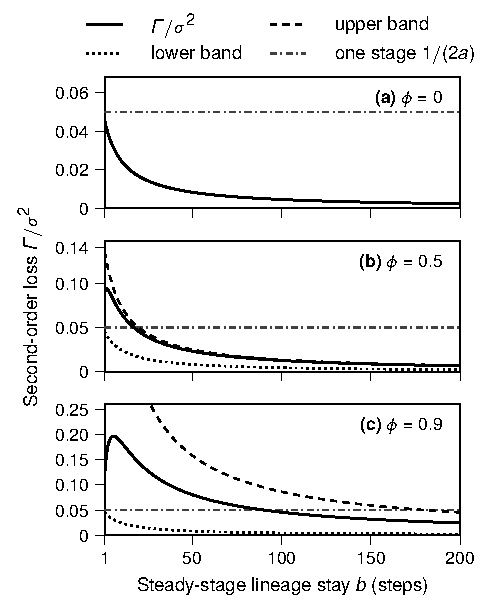
\includegraphics[width=84mm]{figures/ring-1.pdf}
\caption{Second-order loss per generation per unit log-host variance, $\Gamma/\sigma^2$, against steady stay $b$ with illustrative fluctuating stay $a = 10$: (a) $\phi = 0$, (b) $\phi = 0.5$, (c) $\phi = 0.9$. Solid curves: Eq.~\eqref{eq:ring-steady}; dotted and dashed curves: lower and upper edges of Eq.~\eqref{eq:ring-band}; dash-dotted lines: one-stage value $1/(2a) = 0.05$. Both edges coincide with the closed form at $\phi = 0$}
\label{fig:ring-1}
\end{figure}

With positive memory, a short steady stage can raise $\Gamma$ above $1/(2a)$ before longer stays send it to zero (Fig.~\ref{fig:ring-1}). The index $E$ describes infinite-horizon Brownian diffusion, not matrix first passage. Its crossing $b_*$ can differ from finite-horizon crossings, and $b_* \to \infty$ as $L \to 0^+$ at fixed $\theta, \sigma^2 > 0$. Worked examples and simulation details are in Online Resource~1.

Parallel alternative hosts at one transfer enter with squared shares \citep{doak1998}. Fluctuating staying can instead yield a gain.

\begin{proposition}[Alternative hosts at one step and fluctuating staying]\label{prop:ring-alt}
Replacing one transfer multiplier of the primitive gain-only ring by $\sum_{m=1}^M \pi_m h_m(t)$ ($\pi_m \ge 0$, $\sum_{m=1}^M \pi_m = 1$) at fixed mean total transfer and independent $\mathrm{AR}(1)$ hosts ($\sigma_m^2$, $0 \le \phi_m < 1$) gives
\begin{equation}
\Gamma_{\mathrm{alt}} = \sum_{m=1}^M \pi_m^2 \sigma_m^2 \left[ \frac{1 + 2\theta_m}{2\mathcal{T}} - \frac{R_m}{1 - R_m} \right], \qquad R_m = \prod_{k=1}^n \frac{1}{1 + \tau_k/\theta_m} \quad (R_m = 0 \text{ at } \phi_m = 0),
\label{eq:ring-alt}
\end{equation}
with per-step remainder $O(\sigma^4)$ along a fixed noise direction (Theorem~\ref{thm:ring-rem-ar1}). Equal shares of $M$ independent equal-variance, equal-memory hosts divide that step's coefficient by $M$, whereas equal shares of variances $\sigma^2$ and $9\sigma^2$ with the original memory multiply it by $2.5$ (and correlated hosts yield the factor $[1 + \rho(M - 1)]/M$ only under equal shares, equal variances, and cross-covariances equal to $\rho$ times the common autocovariance). Conversely, multiplying a positive staying contribution ($m_k > 0$) by a lognormal $\mathrm{AR}(1)$ factor ($\varsigma^2 > 0$, $0 \le \psi < 1$) at fixed transfers gives per-step cost $\varsigma^2[e_k^2(1 + 2\theta)/2 - e_k\psi m_k / \{(1 - \psi m_k)(1 - R)\}]$ ($e_k = (\tau_k - 1)/\mathcal{T}$; $\theta, R$ at $\psi$), which is negative when $\psi m_k / [(1 - \psi m_k)(1 - R)] > e_k(1 + 2\theta)/2$.
\end{proposition}

\begin{remark}\label{rem:ring-joint-stay}
When transfer into and staying inside a host of stay $b$ are driven jointly by one $\mathrm{AR}(1)$ innovation as in Appendix~\ref{app:ring} (reproduced independently), the coefficient grows as $\kappa^2(1 - \phi^2)b/2$ as $b \to \infty$ without being monotone or bounding bounded-probability host mortality.
\end{remark}

\subsection{Cyclic and periodic hosts, and continuous time}\label{subsec:ring-cyclic}

For cyclic or seasonal hosts, the host spectral density weights a demographic frequency-response function $K(\omega)$ \citep{tuljapurkar1985,bacaer2007}.

\begin{proposition}[Quasi-cycles and spectral response]\label{prop:ring-spectrum}
For one unit-sensitivity transition of a finite primitive model with renewal gap $L_e$ of mean $\mathcal{T}_e = \E[L_e]$:
\begin{enumerate}
\item[(a)] If the autocorrelation is the finite real-valued mixture $\rho(\ell) = \sum_{j=1}^{J} B_j z_j^\ell$ ($\ell \ge 1$, $|z_j| < 1$), $C = S_0/(2\mathcal{T}_e^2) - \mathcal{T}_e^{-1}\sum_j B_j R_e(z_j)/[1 - R_e(z_j)]$ with $S_0 = 1 + 2\sum_j B_j z_j/(1 - z_j)$ and $R_e(z) = \E[z^{L_e}]$ (specializing to $X_t = 2r_c\cos\omega_0\,X_{t-1} - r_c^2 X_{t-2} + \text{noise}$, $0 < r_c < 1$, $0 < \omega_0 < \pi$, via $z = r_c\ee^{\mathrm{i}\omega_0}$, $\rho(1) = 2r_c\cos\omega_0/(1 + r_c^2)$, $B = 1 + \mathrm{i}[\cos\omega_0 - \rho(1)/r_c]/\sin\omega_0$, and weights $B/2, \bar{B}/2$).
\item[(b)] If the driver has spectral density $f(\omega)$ on $(0,\pi)$ with $\pi^{-1}\int_0^\pi f(\omega)\dd\omega = 1$, put $g(\omega) = \E[\ee^{\mathrm{i}\omega L_e}]$. Then
\begin{equation}
C = \frac{1}{\pi}\int_0^\pi f(\omega) K(\omega)\dd\omega, \qquad K(\omega) = -\frac{1}{\mathcal{T}_e}\operatorname{Re}\frac{g(\omega)}{1 - g(\omega)}.
\label{eq:ring-spectrum}
\end{equation}
\item[(c)] On $(0,\pi)$, $K(\omega)$ has mean $1/(2\mathcal{T}_e^2)$ and limit $\lim_{\omega \to 0} K(\omega) = (1 - \mathrm{CV}^2)/(2\mathcal{T}_e)$ ($\mathrm{CV}^2 = \Var(L_e)/\mathcal{T}_e^2$). For one-stage transfer $K(\omega) = 1/(2\tau^2)$ is constant; for $n \ge 2$ in a primitive ring $\lim_{\omega \to 0} K(\omega) > 1/(2\mathcal{T}_e^2)$; $K(\omega) < 0$ if and only if $\operatorname{Re} g(\omega) > |g(\omega)|^2$; and $K(\omega)$ need not be monotone in $\omega$.
\end{enumerate}
\end{proposition}

\begin{figure}
\centering
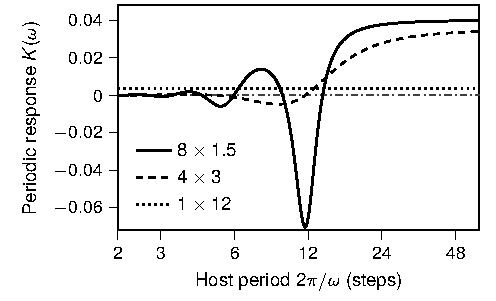
\includegraphics[width=84mm]{figures/ring-2.pdf}
\caption{Periodic response $K(\omega)$ against host period $2\pi/\omega$ (steps), from Eq.~\eqref{eq:ring-spectrum}, for illustrative primitive rings with $\mathcal{T} = 12$ steps. Stays: eight of $1.5$ (solid), four of $3$ (dashed), and one of $12$ (dotted, also the frequency average $1/(2\mathcal{T}^2) \approx 0.00347$). Thin dash-dotted line: $K = 0$}
\label{fig:ring-2}
\end{figure}

Formally, a sinusoidal multiplier $1 + \epsilon\cos(\omega t)$ ($|\epsilon| < 1$, $\omega \notin \pi\mathbb{Z}$) changes growth by $-(\epsilon^2/2)K(\omega)$ to second order ($\epsilon^2$ at period two, with a possible cubic term at period three). Concentrating circuit times around the host period can give $K(\omega) < 0$ (Fig.~\ref{fig:ring-2}). Numerical examples and the $\mathrm{AR}(2)$ check are in Online Resource~1.

In continuous time, a single fluctuating transfer has no cost in a one-stage cycle, while longer cycles retain a second-order cost (Proposition~\ref{prop:ring-ct}, Appendix~\ref{app:ring}).

Here ``one stage'' means one differential equation. No remainder bound is proved for this continuous-time lognormal family (example in Online Resource~1).

\subsection{Remainder theorems}\label{subsec:ring-remainder}

Bounded-perturbation analyticity \citep{ruelle1979}, independent invertible-matrix theorems \citep{lepage1989,hennion1991}, and compact-environment results \citep{steinsaltz2011} omit correlated lognormal multipliers on possibly singular primitive matrices. Reproductive-value normalization \citep{engen2013} gives fourth-order bounds in discrete time.

For a fixed primitive ring with Gaussian autoregressive hosts and sufficiently small noise, the error after the quadratic term is bounded by a constant times the fourth power of noise amplitude (Theorem~\ref{thm:ring-rem-ar1}, Appendix~\ref{app:ring}). The same error bound holds uniformly on compact families of primitive mean matrices (Lemma~\ref{lem:ring-rem-uniform}, Appendix~\ref{app:ring}). It also covers Gaussian linear processes built from absolutely summable weights on past innovations, including linked drivers (Theorem~\ref{thm:ring-rem-lin}, Appendix~\ref{app:ring}).

These bounds yield no usable numerical constants and no uniform control near non-primitivity, closing spectral gaps, host autocorrelations approaching $\pm1$, or growing $n$, nor was Lemma~\ref{lem:ring-rem-uniform} extended to general linear processes.

\subsection{Density dependence in transfers and the \texorpdfstring{$n$}{n}th root}\label{subsec:ring-density}

We test whether counting every transfer as a birth ($R_0^{1/n}$) calms endemic dynamics \citep{dobson2020} in a deterministic constant-host ring with donor-stage transfer regulation.

\begin{proposition}[Deterministic regulated loop]\label{prop:ring-reg}
In $\dd x_{k+1}/\dd t = c_k f_k(x_k) x_k - a_{k+1} x_{k+1}$ ($k$ modulo $n$, $c_k, a_k > 0$, $R_0 = \prod_{k=1}^n (c_k / a_k) > 1$), let each $f_k$ be differentiable, positive, nonincreasing, with $f_k(0) = 1$. Assume an equilibrium $\mathbf{x}^* > \mathbf{0}$ exists, and set $\kappa_k = -x_k^* f_k'(x_k^*)/f_k(x_k^*) \ge 0$ and $G = \prod_{k=1}^n (1 - \kappa_k)$.
\begin{enumerate}
\item[(a)] Eigenvalues at $\mathbf{x}^*$ solve $\prod_{k=1}^n (z + a_k) = G\prod_{k=1}^n a_k$; if $|G| < 1$, $\mathbf{x}^*$ is locally asymptotically stable for all $a_k > 0$.
\item[(b)] At equal exit rates $a_k = a = n/\tau$, eigenvalues are $a(\zeta - 1)$ ($\zeta^n = G$), giving return rate $a(1 - G^{1/n})$ for $0 < G < 1$, instability for $G > 1$, and for $G < 0$ stability when $n = 1, 2$ or $|G| < \sec^n(\pi/n)$ ($n \ge 3$) and instability when $|G| > \sec^n(\pi/n)$ \citep{tyson1978,thron1991,arcak2006}.
\item[(c)] Under $a_k = n/\tau$, $f(x) = \ee^{-x/K}$ in one transfer gives $G = 1 - \ln R_0$, stable for all $R_0 > 1$ at $n = 1, 2$ and critical $\ln R_0 = 1 + \sec^n(\pi/n)$ at $n \ge 3$ ($9, 5, 3.885$ for $n = 3, 4, 5$, approaching $2$). With $\ee^{-x_k/K}$ in every transfer and equal $a, c, K$ at $x_k^* = K\ln R_0 / n$ ($s = \ln R_0 / n$), return rate is $\ln R_0 / \tau$ for $s \le 1$, and critical $\ln R_0$ is $2n$ (even $n$) or $n[1 + \sec(\pi/n)]$ (odd $n \ge 3$), exceeding the one-transfer threshold for all $n \ge 4$ \citep{smith1987,muller2006,strelkowa2010}; for even $n$, alternating equilibria $s \pm d$ ($d = s\tanh(d/2) > 0$) are locally stable just above $s = 2$.
\item[(d)] Renaming $R_0$ as $R_0^{1/m}$ by counting $m$ births alters no stability threshold.
\end{enumerate}
\end{proposition}

\begin{remark}\label{rem:ring-reg-odd}
Equal exit rates are essential in part~(c). For odd $n \ge 3$ under shared exponential regulation, a simple pair crosses transversely at $s = 1 + \sec(\pi/n)$ with negative first Lyapunov coefficient by a referee-supplied rational formula. Independent checks and an unequal-rate example are in Online Resource~1. Alternative functional forms are noted in Appendix~\ref{app:ring}.
\end{remark}

Taking an $n$th root changes neither invasion nor endemic stability. For independent hosts with nonnegative memory on a fixed primitive gain-only ring, the second-order penalty depends on residence times and exposure. At fixed mean total transfer, equal-share independent alternatives with matched variance and memory reduce a transfer's coefficient. Steady stays and cyclic drivers have the conditional effects above. These results concern coefficients. Host feedback raises a separate stability problem (Section~\ref{sec:dyn}).

\section{Bounds at any noise level, \texorpdfstring{$R_0$}{R0} in a random environment, and the lineage identity}\label{sec:bounds}

\paragraph{In brief.}
When host fluctuations have stable long-run statistics (conditions in Proposition~\ref{prop:bounds-any}), the linear rare-parasite ring gives an upper bound on threshold loss at every noise level. Environments independent in time cannot increase growth above the arithmetic-mean baseline. These results separate conclusions that hold for large fluctuations from those that require small noise.

Host fluctuations can be too large for second-order approximations. We therefore derive bounds at every noise amplitude and connect them to lineage sampling and the random-environment reproduction number $R_0^*$. Proofs are in Appendix~\ref{app:bounds}, with verification details in Online Resource~1.

\subsection{Bounds at any noise level, temporal independence, and the two means}\label{subsec:bounds-any}

The variational path principle \citep{dombry2011,kobayashi2017,sughiyama2019}, evaluated along two environment-independent Markov chains, bounds ring growth and threshold loss without small noise or geometric memory.

\begin{proposition}[All-noise ring bounds and equality cases]\label{prop:bounds-any}
Consider an $n$-stage ring with fixed staying contributions $0 \le s_k < 1$, baseline transfers $g_k > 0$, positive multipliers $h_k(t) > 0$ such that $(h_1(t), \dots, h_n(t))$ is jointly stationary and ergodic with $\E|\ln h_k(0)| < \infty$, and a positive initial amount in every stage ($x_k(0) > 0$). Set $\ell_k = -\E\ln h_k(0)$, $R_0 = \prod_{k=1}^n g_k/(1 - s_k)$, $\prod_{k=1}^n (\lambda - s_k) = \prod_{k=1}^n g_k$, $\mathcal{T} = \sum_{k=1}^n (1 - s_k/\lambda)^{-1}$, and $\mathcal{T}_0 = \sum_{k=1}^n (1 - s_k)^{-1}$.
\begin{enumerate}
\item[(a)] The long-run log growth rate $r = \lim_{t \to \infty} t^{-1}\ln X(t)$ exists almost surely, does not depend on the positive initial vector, and satisfies
\begin{equation}
r \ge \ln\lambda - \frac{1}{\mathcal{T}}\sum_{k=1}^n \ell_k, \qquad r \ge \frac{1}{\mathcal{T}_0}\left(\ln R_0 - \sum_{k=1}^n \ell_k\right).
\label{eq:bounds-growth}
\end{equation}
When $\E h_k(0) = 1$, $\ell_k \ge 0$ and $\mathbf{A}_0$ is the arithmetic-mean matrix; at any zero-growth divisor $R_0^*$ on $m$ counted birth transfers, $D = \ln R_0 - m\ln R_0^* \le \sum_{k=1}^n \ell_k$. For mean-one lognormal multipliers $h_k(t) = \exp(\sigma_k z_k(t) - \sigma_k^2/2)$ with unit-variance $z_k$, $\ell_k = \sigma_k^2/2$ for every autocorrelation, so $\mathcal{T}(\ln\lambda - r) \le \sum_{k=1}^n \sigma_k^2/2$, $D \le \sum_{k=1}^n \sigma_k^2/2$, and $\ln R_0 > \sum_{k=1}^n \sigma_k^2/2$ suffices for rare-parasite growth.
\item[(b)] For $n = 1$, $r = \E\ln(s_1 + g_1 h_1(0))$ exactly for any host memory, and $D$ solves $\E\ln[s_1 + (1 - s_1)\ee^D h_1(0)] = 0$. For any $n$ and any environment, $\liminf_{t \to \infty} t^{-1}\ln X(t) \ge \ln\max_k s_k$ whenever $\max_k s_k > 0$.
\item[(c)] Without staying ($s_k = 0$ for all $k$), both inequalities in Eq.~\eqref{eq:bounds-growth} and $D = \sum_{k=1}^n \ell_k$ hold with equality if the environment is ergodic under the $n$-step shift (mixing suffices), whereas one-step ergodicity alone does not suffice (for $n = 2$, $s_1 = s_2 = 0$, $g_1 = g_2 = 1$, and random-phase alternation between $(1.8, 0.2)$ and $(0.2, 1.8)$, $r = \ln 1.8$ exceeds the proposed equality value). Staying does not rule out equality across all stationary ergodic environments: in a two-stage ring with $s_1 \in [0, 1)$, $s_2 = 0$, independent standard Gaussians $Z_t$, $h_1(t) = \exp(\sigma Z_t - \sigma^2/2)$, and $h_2(t) = \exp(-\sigma Z_{t-1} - \sigma^2/2)$, $D = \sigma^2 = \ell_1 + \ell_2$ for every $s_1 \in [0, 1)$.
\end{enumerate}
\end{proposition}

\begin{figure}
\centering
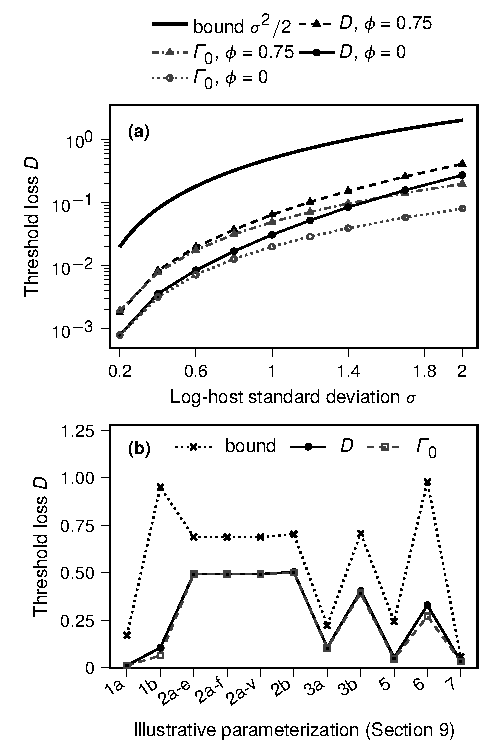
\includegraphics[width=84mm]{figures/bounds-1.pdf}
\caption{Simulated threshold loss $D$, second-order threshold approximation $\Gamma_0$, and all-noise upper bound $\sum_k \sigma_k^2/2$ in discrete-time lognormal $\mathrm{AR}(1)$ rings (simulation details in Online Resource~1). Panel~(a) shows stays $(1, 24)$ on a logarithmic vertical axis across $0.2 \le \sigma \le 2.0$ for $\phi = 0$ (simulated $D$, filled circles and solid line, and $\Gamma_0$, open circles and dotted line) and $\phi = 0.75$ (simulated $D$, filled triangles and dashed line, and $\Gamma_0$, open triangles and dash-dotted line), against the upper bound $\sigma^2/2$ (thick solid curve). Panel~(b) shows all 11 illustrative real-system parameterizations from Section~\ref{sec:num} in saved case order, comparing simulated $D$ (filled circles and solid line), second-order $\Gamma_0$ (open squares and dashed line), and the bound $\sum_k \sigma_k^2/2$ (crosses and dotted line), with connecting lines guiding the eye across categorical cases and simulation standard errors ($\le 0.0007$) smaller than the symbols}
\label{fig:bounds-1}
\end{figure}

Stage durations do not enter the worst-case bound, which cannot be sharpened over all stationary ergodic environments. Simulated cycles with a long steady stage remained below it at large noise, while exceeding $\Gamma_0$ (Fig.~\ref{fig:bounds-1}). This comparison does not prove $\Gamma_0 \le D$ at every noise level. The 161-case campaign and worked values are in Online Resource~1.

Temporal independence of the whole projection matrix rules out growth above the arithmetic-mean matrix baseline \citep{cohen1979b,tuljapurkar1990}.

\begin{proposition}[Environments independent in time give nonnegative loss]\label{prop:bounds-iid}
Let $\mathbf{x}(0)$ be an almost surely nonzero nonnegative vector with finite expectation, and let $(\mathcal{F}_t)_{t\geq0}$ be a filtration such that $\mathbf{x}(0)$ is $\mathcal{F}_0$-measurable, $\mathbf{A}(t)$ is $\mathcal{F}_{t+1}$-measurable, and $\E[\mathbf{A}(t)\mid\mathcal{F}_t]=\mathbf{A}_0$ for all $t\geq0$ with finite nonnegative $\mathbf{A}_0$ (in particular, when $\mathbf{x}(0)$ and $\mathbf{A}(0),\mathbf{A}(1),\dots$ are mutually independent with mean $\mathbf{A}_0$). Then $\E\mathbf{x}(t)=\mathbf{A}_0^t\E\mathbf{x}(0)$ and $\limsup_{t\to\infty}t^{-1}\ln\|\mathbf{x}(t)\|_1\leq\ln\spr(\mathbf{A}_0)$ almost surely, with $\ln0=-\infty$. For a restoring birth multiplier $\ee^y$ relative to a mean threshold, assume additionally that for every $y<0$ the tilted matrices $\mathbf{A}_y(t)$ are $\mathcal{F}_{t+1}$-measurable with $\E[\mathbf{A}_y(t)\mid\mathcal{F}_t]=\mathbf{A}_0(y)$ and $\spr(\mathbf{A}_0(y))<1$. Every finite zero-growth root then has $\Delta\geq0$. In particular, $D\geq0$ in the fixed-staying ring at every existing root $R_0^*$.
\end{proposition}

\begin{remark}\label{rem:bounds-pairwise}
Proposition~\ref{prop:bounds-iid} allows arbitrary same-step dependence among entries of $\mathbf{A}(t)$ and does not assert strict positivity $D > 0$. However, zero autocorrelation of each host at nonzero lags does not replace independence of the whole matrix from its past. In Appendix~\ref{app:bounds} we record a strictly positive two-stage matrix family driven by fair signs that are pairwise independent across all distinct times yet dependent in triples, for which $r = \sigma^3/3 + O(\sigma^4) > 0 = \ln\lambda(\mathbf{A}_0)$ for small $\sigma > 0$ (derived once in referee checks).
\end{remark}

Together, Propositions~\ref{prop:bounds-any} and~\ref{prop:bounds-iid} show why comparisons depend on which mean host abundance is held fixed.

Effective circuit reproduction is bounded below by its geometric-mean-host value and, under temporal independence, above by its arithmetic-mean-host value (Corollary~\ref{cor:bounds-means}, Appendix~\ref{app:bounds}).

Without staying in a mixing environment, effective circuit reproduction equals the geometric-mean-host value. With staying and temporally independent matrices, it lies between the geometric- and arithmetic-mean-host values. These bounds do not imply monotonicity as a stay changes. Field comparisons therefore require a specified common mean (numerical examples in Online Resource~1).

\subsection{The reproduction number in a random environment}\label{subsec:bounds-r0star}

\citet{bacaer2013} characterize reproduction in a finite-state Markov environment by the common birth divisor that reduces long-run growth to zero. We use this characterization to define $R_0^*$ in the Gaussian ring.

\begin{proposition}[Existence, invariance, and threshold expansion of $R_0^*$]\label{prop:bounds-r0star}
Fix staying contributions $0 \le s_k < 1$ ($n = 1$, or $n \ge 2$ with at least one $s_k > 0$), mean transfers $g_k > 0$, mean-one lognormal multipliers from stationary Gaussian $\mathrm{AR}(1)$ drivers ($|\phi_k| < 1$), and $1 \le m \le n$ transfers counted as births.
\begin{enumerate}
\item[(a)] Without noise, the next-generation reproduction number $\spr(\mathbf{F}(\mathbf{I} - \mathbf{V})^{-1})$ is $R_0^{1/m}$, with threshold $R_0 = 1$ for every $m$, and $\ln\lambda = \ln R_0 / \mathcal{T}_0 + O((\ln R_0)^2)$ as $\ln R_0 \to 0$ at fixed stays (exact at every $R_0$ when $n = 1, s_1 = 0$).
\item[(b)] There exists a unique divisor $R_0^* > 0$ on the $m$ birth transfers at which $r = 0$, the population grows when rare ($r > 0$) if and only if $R_0^* > 1$, and
\begin{equation}
m\ln R_0^* = \ln R_0 - D,
\label{eq:bounds-r0star}
\end{equation}
where $D$ depends only on the stays $s_k$ and the joint driver law, and depends neither on the mean transfers $g_k$ nor on $m$.
\item[(c)] Scaling noise along a fixed direction $\sigma_k = \sigma\eta_k$ (with $s_k$, $\eta_k$, driver assignments, and $\phi_k$ fixed), put $\tau_{k,0} = 1/(1 - s_k)$ and $\mathcal{T}_0 = \sum_{k=1}^n \tau_{k,0}$, and let $\Gamma_0 = \mathcal{T}_0 C_0 \sigma^2$ be the second-order per-generation loss evaluated at $\lambda = 1$. Then $D = \Gamma_0 + o(\sigma^2)$ by convexity alone, and $|D - \Gamma_0| \le K'\sigma^4$ for $|\sigma| \le \sigma_0$ by Lemma~\ref{lem:ring-rem-uniform}. For independent hosts with $0 \le \phi_k < 1$,
\begin{equation}
\Gamma_0 = \sum_{k=1}^n \sigma_k^2 \left[ \frac{1 + 2\theta_k}{2\mathcal{T}_0} - \frac{R_{k,0}}{1 - R_{k,0}} \right], \qquad R_{k,0} = \prod_{j=1}^n \frac{1}{1 + \tau_{j,0}/\theta_k} \quad (R_{k,0} = 0 \text{ at } \phi_k = 0).
\label{eq:bounds-gamma0}
\end{equation}
\end{enumerate}
\end{proposition}

Counting all transfers as births divides $\ln R_0$ and $D$ equally, leaving the invasion threshold unchanged. Away from $R_0 = 1$, $\Gamma_0$ uses threshold stays $\tau_{k,0} = (1 - s_k)^{-1}$, not lineage stays $\tau_k = (1 - s_k/\lambda)^{-1}$. Transfer invariance of $D$ does not extend to growth variance $V$. A numerical check is in Online Resource~1. In continuous time, this formal normalization matches \citet{bacaer2007} at a single frequency, without a proved remainder.

\subsection{Lineage representation, the variance identity, and its literature status}\label{subsec:bounds-lineage}

Weighting each transition's expected logarithmic penalty $\ell_e = -\E\ln h_e(0)$ by how often a reference lineage uses it gives an upper bound on growth loss for general life cycles (Proposition~\ref{prop:bounds-path}, Appendix~\ref{app:bounds}). The gap $\ell_e$ equals $\sigma_e^2/2$ (transition log standard deviation $\sigma_e$) unconditionally only for mean-one lognormal multipliers (counterexample in Online Resource~1).

To second order, growth loss equals this visit-weighted bound minus half the within-environment variance rate among coexisting lines of descent, so differing lineage histories reduce the penalty (Theorem~\ref{thm:bounds-lineage}, Appendix~\ref{app:bounds}).

The lineage variance in Theorem~\ref{thm:bounds-lineage} is the within-environment variance among reference lineages, averaged over environments and expressed as a long-run rate. It differs from population growth-rate variance and requires primitivity. Simulations agreed within sampling error across eight primitive models (details in Online Resource~1). Comparing life cycles requires a common unit for loss, because the mean penalty, generation time, and mean matrix can all change.

\paragraph{Literature status.}
We claim no priority or new mathematics for Proposition~\ref{prop:bounds-path} or Theorem~\ref{thm:bounds-lineage}. The former is a direct corollary of published results, and the latter rewrites a published perturbation coefficient. The reference chain and edge elasticities appear in \citet{bienvenu2017}, path representations and Jensen bounds in \citet{dombry2011,kobayashi2015,kobayashi2017}, and lineage cumulant expansions in \citet{nozoe2017,levien2020a,genthon2021,yamauchi2022}. The random-environment coefficient is due to \citet{tuljapurkar1982a,tuljapurkar1990,tuljapurkar2006}. Our 28-work review did not find Eq.~\eqref{eq:bounds-lineage} in this variance form with its total-variance equivalence to $C''$. Three supplements and four full texts remained unavailable. The reading record and related literature are in Online Resource~1.

For a parasite in the fixed-staying ring, the aggregate threshold loss satisfies $D\leq\sum_k\ell_k$ at every noise amplitude. With no staying, equality requires ergodicity under the cycle-length shift and gives geometric-mean-host reproduction. At small noise, residence times, parallel routes, and spatial structure reduce the penalty only insofar as coexisting lineages sample different times or host states within the same environment.

\section{Extensions and the limits of each conclusion}\label{sec:mech}

\paragraph{In brief.}
How much storage protects a parasite depends on how it waits, survives, and meets its hosts. Each of these is examined separately below, with exact results where available and small-noise comparisons elsewhere. A long sheltered stage does not guarantee protection when waiting deaths, linked host fluctuations, or host absences change the comparison.

An additional host can alter transmission success, waiting times, and the environments encountered by descendants. These comparisons test where the storage argument of \citet{dobson2020} holds. Loss of reproduction remains distinct from extinction of a finite population.

Unless stated otherwise, the baseline fixes rates at their arithmetic means. Rings are calibrated to that threshold, counting one birth per circuit. We write \(D_2=\sigma^2K\) for quadratic loss. In route networks, \(\Delta\) is the log multiplier on specified reproductive returns that restores zero growth, so loss depends on the birth convention (Section~\ref{sec:model}). Examples are illustrative. Proofs are in Appendix~\ref{app:mech}; ``refereed'' denotes the internal review described in Section~\ref{sec:model}.

\subsection{Scarcity that delays transmission}
The original ring loses individuals that leave but fail to transfer. In a contact-limited stage, host scarcity instead prolongs waiting, during which individuals can die. Let the death probability be \(\mu\), encounter probability \(ch_t\), and yield per encounter \(b_j\), where \(\mathbb E h_t=1\). Then
\begin{equation}\label{eq:mech-contact-model}
 s_j(t)=1-\mu-ch_t,\qquad g_j(t)=b_jch_t,
 \qquad d=\frac{\mu}{\mu+c}.
\end{equation}
The constraint \(\mu+ch_t\leq1\) excludes an unbounded lognormal host for every \(c>0\). The death fraction \(d\) applies at the constant-mean-host threshold, and need not match the fraction under correlated fluctuations.

\begin{proposition}[Contact limitation]\label{prop:mech-contact}
Let the mean ring be primitive, with positive transfers and positive baseline staying in stage \(j\). Let \(h_t=1+\sigma\xi_t\), where \(\xi\) is bounded, stationary ergodic, centered, has unit variance, and has covariance \(\phi^{|\ell|}\), \(-1<\phi<1\). Keep every changed contribution positive for sufficiently small \(|\sigma|\). Put
\begin{equation}\label{eq:mech-contact}
 \theta=\frac{\phi}{1-\phi},\quad q_k=\frac{\phi}{\phi+(1-\phi)\tau_k},\quad
 R=\prod_kq_k,\quad K_g=\frac{1+2\theta}{2\mathcal T}-\frac{R}{1-R}.
\end{equation}
At \(\phi=0\), set \(q_k=R=0\). Then
\begin{equation}\label{eq:mech-contact-coefficient}
 D_2=\sigma^2K_c,\qquad K_c=d^2K_g+d(1-d)\frac{q_j-R}{1-R}.
\end{equation}
The remainder is \(O(|\sigma|^3)\), or \(O(\sigma^4)\) if the whole driver process is invariant under sign reversal. For \(0\leq\phi<1\) and \(0<d\leq1\), \(K_c>0\). At \(d=0\), reproductive value is conserved and \(D=0\) at every admissible amplitude. The value \(d=1\) denotes the gain-only perturbation, with the staying perturbation omitted. If a different steady stay tends to infinity with the other stays, \(d\), and memory fixed, then
\begin{equation}\label{eq:mech-contact-limit}
 \lim K_c=d(1-d)q_j.
\end{equation}
\end{proposition}
The coefficient was proved and refereed; its bounded-forcing remainder is derived separately in Appendix~\ref{app:mech-contact}. Without memory, contact limitation multiplies the gain-only coefficient by \(d^2\). Positivity fails with negative memory, and the long-stay value is a limit, not a floor (Fig.~\ref{fig:mech-1}; details in Online Resource 1). The continuous-time expansion replaces \((1+2\theta)/(2\mathcal T)\) by \(\theta/\mathcal T\), so the discrete no-memory factor does not extend to a rapidly changing continuous-time host. Storage therefore depends on mortality while awaiting transmission.

\begin{figure}\centering
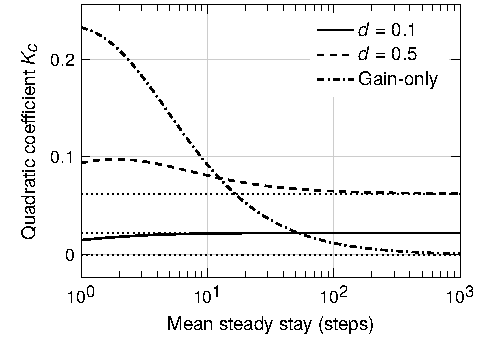
\includegraphics[width=84mm]{figures/mech-1.pdf}
\caption{Contact-limited quadratic loss coefficient against the mean steady stay, with contact stay three and memory \(\phi=0.5\). Solid, dashed, and dash-dotted curves denote \(d=0.1\), \(d=0.5\), and gain-only transmission. Dotted horizontal lines mark the corresponding long-stay limits, including zero for gain-only transmission. These are coefficients of host variance, not finite-noise losses}\label{fig:mech-1}
\end{figure}

\subsection{The distribution of time spent in a stage}
Equal mean stays need not provide equal protection. A sheltered segment has a kernel (expected output at each lag after entry, including survival and reproduction). Equal kernels and unchanged exposed dynamics preserve the growth exponent and threshold, regardless of compartment names. Dividing a stay generally changes its kernel \citep{blythe1984,lloyd2001}.

\begin{proposition}[Renewal time and stay shape]\label{prop:mech-renewal}
Consider a finite primitive reference model at the mean-rate threshold, with the marked regenerative transfer as the sole counted birth. Its frequency is \(b=1/\mathcal T\). Here \(K\) denotes the coefficient of the restoring multiplier \(\Delta\), equal to \(D_2/\sigma^2\) in a ring with one counted birth per circuit. All rates are constant except that transfer, multiplied by \(\exp(\sigma\xi_t-\sigma^2/2)\), with centered stationary unit-variance Gaussian AR(1) driver, \(0\leq\phi<1\). Assume the local perturbation expansion applies. Let \(L\) be the positive integer return time between uses of that event by the reference lineage, \(\mathcal T=\mathbb E L\), and \(R=\mathbb E[\phi^L]\). Then
\begin{equation}\label{eq:mech-renewal}
 K=\frac{1+2\theta}{2\mathcal T}-\frac{R}{1-R},\qquad
 K<0\ \Longleftrightarrow\ R>\frac{1+2\theta}{1+2\theta+2\mathcal T}.
\end{equation}
At fixed \(\mathcal T\) and \(0<\phi<1\), a mean-preserving spread in convex order lowers \(K\). For a death-free steady stay of mean \(b\) represented by \(m\) equal geometric substages, integer \(1\leq m\leq b\), its transform is \((1+b/(m\theta))^{-m}\). Increasing \(m\) strictly raises \(K\) when \(\phi>0\), provided all compared models remain primitive. At \(\phi=0\), \(K=1/(2\mathcal T)\). A sum of geometric stays cannot satisfy the gain condition.
\end{proposition}
This result was proved and refereed. The return-time transform, rather than variance alone, orders the coefficients. Rare long returns can give \(K<0\), while a fixed sheltered delay after a geometric exposed stay of mean \(a>1\) makes \(K\to0\) at fixed memory. Neither conclusion locates a finite-noise threshold. Worked examples are in Online Resource 1. Mortality during a fixed delay incurs its full survival cost (Lemma~\ref{lem:mech-mortality}).

\begin{proposition}[Every stay fixed]\label{prop:mech-fixed}
Suppose every stay is fixed, the cycle has \(n\) time positions, and one transfer has a positive stationary multiplier \(h\) with \(\mathbb E|\log h|<\infty\). If the environment is ergodic under the shift by \(n\) steps, then \(D=-\mathbb E\log h\). In particular, for the mean-one lognormal multiplier, \(D=\sigma^2/2\), regardless of the fixed durations.
\end{proposition}
This separate cohort proof was refereed. An all-fixed cycle with \(n>1\) is not primitive, so the preceding expansion cannot be substituted there. Both mean duration and its spread matter (Fig.~\ref{fig:mech-4}).

\begin{figure}\centering
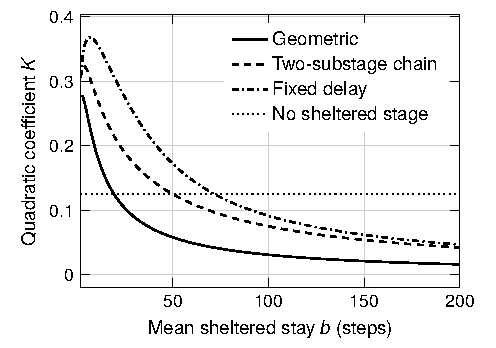
\includegraphics[width=84mm]{figures/mech-4.pdf}
\caption{Quadratic loss coefficients for a geometric exposed stay of four steps and a sheltered stay of mean \(b\), at \(\phi=0.9\). Solid, dashed, and dash-dotted curves give a geometric sheltered stay, two equal geometric substages, and a fixed delay. The dotted horizontal line gives the no-sheltered-stage coefficient. Fixed delays are evaluated at integer steps, and the exposed stay remains random in every comparison}\label{fig:mech-4}
\end{figure}

\subsection{Temperature-dependent completion and development}
Temperature affects development and death, requiring joint treatment of staying and transfer. Physical shelter from temperature differs from buffering host abundance \citep{kutz2014,aleuy2020}. 

Changing stage-leaving speed (the developmental clock) alone leaves the threshold unchanged when completion probabilities (successful completion among leavers) are constant; joint thermal changes in both can alter the quadratic sign (Proposition~\ref{prop:mech-thermal}, Appendix~\ref{app:mech}).
These statements were proved and refereed. Conservation requires constant completion probabilities in every exposed stage. A clock-sensitive stage remains exposed when another stage has temperature-dependent completion. No finite-amplitude remainder bound is supplied; an illustrative numerical comparison is in Online Resource 1.

When staying rates fluctuate, their logarithmic penalties also enter the bound, weighted by time spent staying (Proposition~\ref{prop:mech-edge-bound}, Appendix~\ref{app:mech}).
This bound was proved and refereed. A temperature-sensitive reservoir must be evaluated through both completion and staying rates (worked example in Online Resource 1).

\subsection{Encounter functions and alternative routes}
Curved encounter functions of host abundance $H$ change both mean transmission at fixed mean host abundance and the quadratic fluctuation response (Proposition~\ref{prop:mech-curvature}, Appendix~\ref{app:mech}).
The derivation was reproduced independently. Smoothness at the mean alone does not imply the required expectation or growth expansion. A saturating type-II encounter cannot give a quadratic benefit when \(K_g\geq0\), whereas an inverse response does so when \(K_g<1\). Bounds concern the rate's logarithmic gap, which for a normalized power \(H^\eta\) (elasticity \(\eta\)) is \(\eta^2\sigma^2/2\).

\begin{proposition}[Alternative, optional, and bypass routes]\label{prop:mech-routes}
Assume every compared mean model is primitive on retained states, calibrated to its own threshold, with fixed staying and the stated mean-one Gaussian AR drivers. In a parallel network, a central stage of stay \(\tau_0\) enters host \(j\) with reproductive share \(w_j\geq0\), \(\sum_jw_j=1\), and host stay \(\tau_j\). Count all returns as births. Without memory, put \(\mathcal T=\tau_0+\sum_jw_j\tau_j\), \(u_j=w_j\kappa_j\), and \(V=\mathbf u^{\mathsf T}\mathbf C\mathbf u\), with \(\mathbf C\) the log-driver correlation matrix. Then
\begin{equation}\label{eq:mech-parallel}
 \Delta_2=\frac{\sigma^2V}{2\mathcal T}.
\end{equation}
A newcomer of share \(0<f\leq1\), variance coefficient \(U\), covariance \(C\) with the old aggregate, and stay difference \(\delta\tau\) lowers this coefficient exactly when
\begin{equation}\label{eq:mech-newcomer}
 f\mathcal T(V-2C+U)<2\mathcal T(V-C)+V\delta\tau.
\end{equation}
For a fraction \(0\leq f\leq1\) using an optional steady host of survival \(0\leq q\leq1\), define \(Y=1-f+fq\), require \(Y>0\), and put \(\alpha=fq/Y\). At equal mean reproduction, \(\mathcal T=\tau_0+\tau_1+\alpha\tau_p\), \(R=q_0q_1(1-\alpha+\alpha q_p)\), and \(K_{\rm opt}\) is \eqref{eq:mech-renewal}. For a bypass of relative yield \(q\geq0\), again with \(0\leq f\leq1\) and \(Y>0\), put \(\alpha=(1-f)/Y\), \(\mathcal T=\tau_0+\alpha\tau_1\), and \(R=q_0(1-\alpha+\alpha q_1)\). Then
\begin{equation}\label{eq:mech-bypass}
 K_{\rm by}=\alpha^2\left[\frac{1+2\theta}{2\mathcal T}-\frac{q_0q_1}{1-R}\right].
\end{equation}
For either route, the exact advantage at fixed other rates is \(\log Y+\Delta_{\rm base}-\Delta_{\rm route}\).
\end{proposition}
These formulas were reproduced independently. Independent alternatives enter through shares squared, whereas independent obligatory transfers add their quadratic terms on the same mean matrix. A noisy newcomer can increase loss. An optional host with \(fq>0\) lowers the no-memory coefficient at equal mean reproduction, but this benefit fails under strict alternation (examples in Online Resource 1). For a single noisy transfer and two equal stays \(a>1\),
\begin{equation}\label{eq:mech-negative-memory}
 K_g=\frac{1}{4a}\frac{1+\phi(1+2/a)}{1-\phi(1-2/a)}<0
 \quad\Longleftrightarrow\quad \phi<-\frac{a}{a+2}.
\end{equation}
Temporal independence therefore cannot be replaced by a variance condition. A strict-alternation example is in Online Resource 1. Relapse also permits gains, as in \citet{white2016}; its continuous-time renewal criterion is in Appendix~\ref{app:mech-renewal}.

\subsection{One host on two transfers and linked hosts}
Transfers responding to the same host or to linked hosts depend on covariances at directed time lags, beyond same-day correlations \citep{tuljapurkar1982a,tuljapurkar2006}. Define
\(\rho_{ij}(\ell)=\mathbb E[\xi_i(t)\xi_j(t-\ell)]\): host \(i\) is observed later. Both transfers read their hosts at the current step.

\begin{proposition}[Linked transfers]\label{prop:mech-linked}
Let a primitive fixed-staying ring at threshold have lognormal transfer multipliers driven by a stable finite-dimensional Gaussian autoregression, or a finite-dimensional Gaussian linear extension of it, centered with unit marginal variances and with the local expansion justified. For transfer sensitivities \(\kappa_i\), let \(u_{j\to i}(\ell)\) be the reference probability of using transfer \(i\) at lag \(\ell\) after transfer \(j\). Then
\begin{equation}\label{eq:mech-linked}
 K=\sum_{i,j}\kappa_i\kappa_j\left[\frac{\rho_{ij}(0)}{2\mathcal T}
 +\sum_{\ell\geq1}\rho_{ij}(\ell)\left(\frac1{\mathcal T}-u_{j\to i}(\ell)\right)\right].
\end{equation}
For two hosts write \(K=K_1+K_2+X\). A net quadratic gain requires \(X<-(K_1+K_2)\), and adding the second host helps relative to the first alone exactly when \(X<-K_2\). For unit sensitivities, exchanging hosts gives
\begin{equation}\label{eq:mech-order}
 K_{12}-K_{21}=-\sum_{\ell\geq1}[\rho_{21}(\ell)-\rho_{12}(\ell)]
 [u_{1\to2}(\ell)-u_{2\to1}(\ell)].
\end{equation}
\end{proposition}
The formulas and specified simulations were reproduced independently. Reversing linked hosts changed the sign of finite-noise loss in the illustrative example (Fig.~\ref{fig:mech-3}; details in Online Resource 1). Reversible cross-covariances or identical directed return distributions eliminate the quadratic order effect; equal mean travel times alone do not.

For one host driving both transfers of a two-stage ring with stays \(a,b\), the same-sign coefficient is
\begin{equation}\label{eq:mech-common}
 K_+=\frac{2ab+\theta[2(a+b)-(a-b)^2]}{(a+b)[ab+\theta(a+b)]}.
\end{equation}
For \(0\leq\phi<1\), it is negative exactly when \((a-b)^2>2(a+b)\) and \(\theta>2ab/[(a-b)^2-2(a+b)]\). At equal stays it is \(1/a>0\). Continuous time lacks the instantaneous cost \((\kappa_1+\kappa_2)^2/(2\mathcal T)\), so equal same-sign sensitivities give a gain for any unequal pair of leaving rates there. Shrinking the time step reconciles the formulas (Appendix~\ref{app:mech-common}). This distinction also matters when interpreting switching host--vector models \citep{watts2021}. Linked hosts can preserve a useful ordering of encounters, but correlation does not supply an unconditional benefit.

\begin{figure}\centering
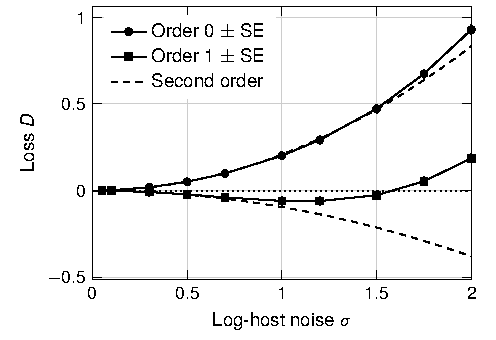
\includegraphics[width=84mm]{figures/mech-3.pdf}
\caption{Loss against log-host noise for two orders of linked hosts on a ring with stays \((5,50,5)\). Circles denote host 1 on transfer 0 and host 2 on transfer 1, squares the reverse order. The host autoregression has radius 0.9 and rotation angle \(\pi/10\). Solid lines join simulation estimates, bars give one standard error, and dashed curves are the respective quadratic predictions. The horizontal dotted line marks zero loss. Transfer 2 is steady}\label{fig:mech-3}
\end{figure}

\subsection{Hosts that can be absent}\label{subsec:mech-absent}
Host absence violates assumption A13. Period-two outages explain the mechanism behind 51 stay reversals in replayed \textit{Tribolium} larval records (Section~\ref{sec:num}).
Here \(a,s\) are finite mean stays, with \(a>1,s\geq1\). Set
\begin{equation}\label{eq:mech-outage-model}
 b=1/a,\quad p=1-b,\quad \varepsilon=1/s,\quad q=1-\varepsilon,
 \qquad \mathbf A_t(c)=\begin{pmatrix}p&\varepsilon c\\b h_t&q\end{pmatrix},\quad c>0.
\end{equation}
The restoring loss is \(D=\log c_*\), where the top matrix growth exponent vanishes at \(c_*\).

\begin{proposition}[Thresholds with absent hosts]\label{prop:mech-outage}
Let \(h_t\geq0\) be stationary ergodic with \(\mathbb E h_t=1\). The threshold exists uniquely and is finite. Temporal independence gives \(D\geq0\). For \(h=(2,0)\) repeated with uniform random phase,
\begin{equation}\label{eq:mech-outage-alt}
 D=\log\frac{(2a-1)(2s-1)}{2((2a-1)s-a+1)}<0,\qquad
 D_s=\frac{1}{(2s-1)((2a-1)s-a+1)}>0.
\end{equation}
If \(\mathbb E h_t^4<\infty\), then, at fixed \(a\) and host law,
\begin{equation}\label{eq:mech-outage-long}
 D=\frac{A}{s}+O(s^{-2}),\qquad
 A=\frac{\operatorname{Var}(h_t)}2+
 \sum_{\ell\geq1}p^{\ell-1}\operatorname{Cov}(h_t,h_{t-\ell}).
\end{equation}
For \(A\ne0\), every fixed \(\kappa>1\) eventually gives
\(\operatorname{sign}[D(a,\kappa s)-D(a,s)]=-\operatorname{sign}A\).
If additionally \(h_t\leq M<\infty\), put \(R=b/(256M^2)\). Then
\begin{equation}\label{eq:mech-outage-sign}
 \operatorname{sign}D_s=-\operatorname{sign}A,\quad
 \operatorname{sign}D=\operatorname{sign}A
 \quad\text{when}\quad
 0<s^{-1}<\min\{R/2,|A|R^2/4\},\quad A\ne0.
\end{equation}
\end{proposition}

With some staying, a finite threshold bound can remain available even when a host is sometimes absent (Proposition~\ref{prop:mech-outage-bound}, Appendix~\ref{app:mech}).
Propositions~\ref{prop:mech-outage} and~\ref{prop:mech-outage-bound} are proved in Appendix~\ref{app:mech-outage} and checked independently. The derivative sign under fourth moments alone remains open. Negative \(A\) shows how longer storage can remove an advantage of alternating host access.

\subsection{Dispersal among patches}
Dispersal changes the host histories encountered by descendants across patches. For the Gaussian host laws and island movement in Proposition~\ref{prop:mech-dispersal}, this can yield a quadratic gain, written $D_2=\sigma^2F<0$, where $F$ is the spatial loss coefficient (Appendix~\ref{app:mech}).
The coefficient was reproduced independently. Simulated gains ended at larger tested amplitudes (Fig.~\ref{fig:mech-2}; details in Online Resource 1). These sampled signs do not establish an interval theorem.

A long steady stage can also remove part of the spatial gain. Its coefficient and sign condition are in Appendix~\ref{app:mech-spatial}. The logarithmic-gap bound survives movement, transit losses, and unequal patch quality when these are included in the baseline. Perfectly synchronous hosts with conservative movement give exactly the aggregate single-patch ring. Movement therefore helps through differing environmental histories; effective variance replacement applies only in restricted small-noise cases.

\begin{figure}\centering
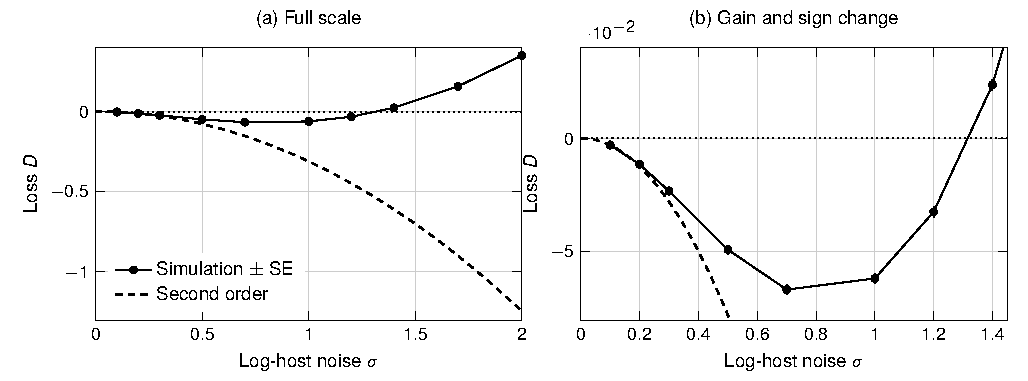
\includegraphics[width=174mm]{figures/mech-2.pdf}
\caption{Dispersal loss for stays \((2,2)\), four independent island patches, movement fraction 0.15 in stage 1, and memory \(\phi=0.8\). Circles joined by a solid line are estimates from random matrix products, bars give one standard error, and the dashed curve is \(\sigma^2F\). Panel (a) shows the full scale and panel (b) enlarges the gain and sign change. The horizontal dotted line marks zero loss. Movement follows demography, and there is no transit mortality}\label{fig:mech-2}
\end{figure}

\subsection{The mechanisms together}
The R16 numerical study combined contact limitation, regularized stays, alternative hosts, asynchronous patches, and storage mortality. It used a bounded two-state host, three illustrative cycles, and two step sizes, with 192 admissible cells. Independent reproduction covered selected cells and all comparison counts. All 18 resolved gains involved patches. Quadratic predictions sometimes had the wrong sign. This comparison combines finite amplitude with a skewed host law outside the standardized small-amplitude family, and has no comparator without a long stage. Details are in Online Resource 1; extinction comparisons and the calibration limitation are in Appendix~\ref{app:mech-r16}.

Table~\ref{tab:mech-summary} collects the model changes and their domains.

\begin{table}[htbp]\centering\scriptsize
\setlength{\tabcolsep}{2pt}
\caption{Summary of the changed models. M denotes arithmetic-mean rates, H constant mean host abundance, and T constant mean temperature. Loss is dimensionless log reproduction per circuit or specified birth. Q denotes quadratic, E exact, and N numerical results. R denotes internal proof review, I independent numerical reproduction, and O one derivation or study. Complete hypotheses are in the cited results, including primitivity for local expansions. Illustrative examples are in Online Resource 1}\label{tab:mech-summary}
\begin{tabular*}{\textwidth}{@{\extracolsep{\fill}}p{0.18\textwidth}p{0.06\textwidth}p{0.09\textwidth}p{0.07\textwidth}p{0.42\textwidth}p{0.08\textwidth}@{}}\toprule
Changed model & Base & Units & Order & Condition & Status\\\midrule
Contact-limited transfer & M & circuit & Q & Proposition~\ref{prop:mech-contact}, \(0\leq\phi<1,d>0\): positive & R\\
Contact, long steady stay & M & circuit & Q & Fixed other stays and memory, limit \(d(1-d)q_j\) & R\\
No waiting deaths & M & circuit & E & Valid threshold contact model, conserved positive value & R/I\\
Renewal stay shape & M & circuit & Q & Proposition~\ref{prop:mech-renewal}, gain iff transform exceeds its threshold & R\\
Fixed delay with random stay & M & circuit & Q/N & \(a>1\), fixed \(0\leq\phi<1\); small noise before long delay & R\\
Every stay fixed & M & circuit & E & Integrable log, ergodic cycle-length shift & R\\
Mortality during storage & M & circuit & Q & Lemma~\ref{lem:mech-mortality}: one noisy transfer, independent environments, survival \(\exp(-\mu)\) per step & R\\
Thermal clocks & M/T & circuit & E/Q & Proposition~\ref{prop:mech-thermal}; conservation needs all completion probabilities constant & R\\
Thermal curvature & T & circuit & Q & Inequality~\eqref{eq:mech-thermal-curvature}, regularity and cross terms retained & R\\
Changing staying edges & M & circuit & E & Proposition~\ref{prop:mech-edge-bound}, finite logs and existing threshold & R\\
Curved encounter & H/M & circuit & Q & Proposition~\ref{prop:mech-curvature}; benefit at H under its curvature criterion & I\\
Alternative hosts & M & birth & Q & Primitive models, no memory, inequality~\eqref{eq:mech-newcomer} & I\\
Optional host & M & birth & Q/E & Proposition~\ref{prop:mech-routes}; strict no-memory benefit needs \(fq>0\) & I\\
Bypass & M & birth & Q/E & Equation~\eqref{eq:mech-bypass}; fixed-rate margin also includes \(\log Y\) & I\\
Negative memory/alternation & M & circuit & Q/E & Primitive equal-stay ring for \eqref{eq:mech-negative-memory}; periodic products separately & I\\
Hosts that can be absent & M & circuit & E & Propositions~\ref{prop:mech-outage} and~\ref{prop:mech-outage-bound}, fixed stays, one fluctuating transfer & R/I\\
One host on two transfers & M & circuit & Q & Discrete condition after \eqref{eq:mech-common}; continuous limit differs & I/O\\
Linked hosts & M & circuit & Q/N & Proposition~\ref{prop:mech-linked}, directed lags and full covariance law & I\\
Dispersal & M & circuit & Q/N & Proposition~\ref{prop:mech-dispersal}; gain under its spatial criterion & I\\
Combined mechanisms & M & birth & N & R16 bounded two-state host, two tested steps, available comparisons only & I\\\bottomrule
\end{tabular*}
\end{table}

Storage can protect a parasite by changing transmission timing and the environmental histories of lineages. Survival, return-time distributions, and linked encounters determine whether protection remains. Host count specifies none of these quantities.

\section{A case solved exactly at every noise level}\label{sec:exact}

\paragraph{In brief.}
For a one-step fluctuating stage followed by a geometric steady stay, independent gamma-distributed host abundance permits an exact calculation. At every fixed positive host variance, lengthening the steady stay strictly reduces the threshold loss in this linear rare-parasite setting. With nonnegative host memory, the decrease is proved only to second order or, for the bounded two-state host, for long stays. Strongly negative memory can reverse it.

Time spent in a steady stage can reduce exposure to fluctuating transmission. Using \citet{roerdink1988}'s exact growth formula for a one-step fluctuating stage and a geometric steady stay, we prove that the threshold loss decreases strictly with the steady stay at every fixed gamma host variance.

\subsection{Model, invariant law, and attribution}\label{subsec:exact-model}

Stage~0 has no staying, and its transfer to stage~1 fluctuates with relative host abundance $h_t$. Stage~1 has staying fraction $s\in(0,1)$, mean stay $\tau=1/(1-s)$ steps, and constant transfer $g_1>0$ back to stage~0. With mean outward transfer $g_0>0$, product $c=g_0g_1>0$, and population vector $\mathbf{x}(t)=(x_0(t),x_1(t))^{\mathsf{T}}$, the map is
\begin{equation}
\begin{gathered}
\mathbf{x}(t+1) = \mathbf{A}(t)\mathbf{x}(t), \qquad
\mathbf{A}(t) = \begin{pmatrix} 0 & g_1 \\ g_0 h_t & s \end{pmatrix},\\
x_1(t+1) = s x_1(t) + c h_t x_1(t-1),
\end{gathered}
\label{eq:exact-matrix}
\end{equation}
where the host multipliers $h_t$ are independent and identically distributed across time steps $t$ according to a gamma law $\operatorname{Gamma}(p, 1/p)$ with shape parameter $p > 0$ and scale parameter $1/p$, so that $\mathbb{E} h_t = 1$ and $\operatorname{Var}(h_t) = 1/p$. All logarithms below are natural. The arithmetic-mean matrix has characteristic equation $\lambda^2 = s\lambda + c$ and deterministic per-circuit reproduction number $R_0 = c/(1-s)$, with mean-matrix threshold $c = 1-s$. Counting one transfer as birth, the stochastic threshold loss $D(s,p)$ is the logarithmic increase in $R_0$ required to restore zero long-run stochastic growth $r(s,c,p)$ from its mean threshold, defined implicitly along with the logarithmic gap $\ell(p)$ and the auxiliary ratio chain $X_t$ by
\begin{equation}
\begin{gathered}
r\bigl(s, (1-s)\mathrm{e}^{D(s,p)}, p\bigr) = 0,\\
\ell(p) = -\mathbb{E}\ln h_t = \ln p - \psi(p), \qquad
X_{t+1} = \frac{Y_{t+1}}{s + X_t},
\end{gathered}
\label{eq:exact-defs}
\end{equation}
where $\psi = \Gamma'/\Gamma$ is the digamma function, $\psi_1 = \psi'$ is the trigamma function (with $\operatorname{Var}(\ln h_t) = \psi_1(p)$), $\gamma$ denotes Euler's constant, $Y_t = c h_t \sim \operatorname{Gamma}(p, \theta)$ with scale $\theta = c/p$ is independent of the past, and $\kappa = s^2/\theta = s^2 p/c$ is the dimensionless ratio parameter. All numerical parameter values below are illustrative properties of this mathematical model rather than measurements on real parasites.

The exact solution is due to \citet{roerdink1988}, who studied the same matrix for biennial life histories with fluctuating recruitment. His equations~3.15a--3.16 give the invariant Kummer density, and his equation~5.6 gives the Tricomi growth formula. The invariant continued-fraction law goes back to \citet{dyson1953}, whose original equations were checked indirectly through later treatments \citep{roerdink1988,marklof2008,letac2010,forrester2021a,forrester2021b}. We use these published results to study the threshold after compensating for changes in the deterministic reproduction number.

An auxiliary population ratio has a unique stationary distribution, which gives the long-run growth rate for every nonzero nonnegative starting population (Proposition~\ref{prop:exact-R1}, Appendix~\ref{sec:exact-app}).

Independent quadrature checks of the growth formula are described in Online Resource~1.

Roerdink's exact growth formula can be evaluated using special functions or convergent series (Proposition~\ref{prop:exact-R2}, Appendix~\ref{sec:exact-app}).

In a general independent-environment ring (Section~\ref{sec:bounds}), Jensen's inequality gives only the weak bounds $0 \le D \le \ell(p)$. For the gamma cycle with interior staying, both inequalities are strict at every noise amplitude (proved in Appendix~\ref{sec:exact-app} and refereed).

\begin{proposition}\label{prop:exact-R3}
For every $s \in (0,1)$ and every $p > 0$, the growth rate $r(s,c,p)$ is continuous and strictly increasing in $c \in (0,\infty)$, with $\lim_{c\downarrow 0} r(s,c,p) = \ln s < 0$ and $\lim_{c\to\infty} r(s,c,p) = \infty$. Consequently, there exists a unique real root $D(s,p)$ of $r(s, (1-s)\mathrm{e}^y, p) = 0$, and it satisfies
\begin{equation}
0 < D(s,p) < \ell(p).
\label{eq:exact-bounds}
\end{equation}
\end{proposition}

Any $s>0$ recovers part of the logarithmic-gap penalty, while variability still imposes a positive cost. Constant survival in the storage stage matters. With gamma noise on the staying entry instead, the companion random-matrix model has $D_{\mathrm{stay}}>0$ and $D_{\mathrm{stay}}\to\infty$ as $s\uparrow1$ at fixed $p$ (Proposition~\ref{prop:exact-R8}; proved and refereed). The unbounded multiplier is not a survival probability; details are in Online Resource~1.

The exact loss and second-order approximation are compared in Fig.~\ref{fig:exact-1}; numerical details are in Online Resource~1.

\begin{figure}[t]
\centering
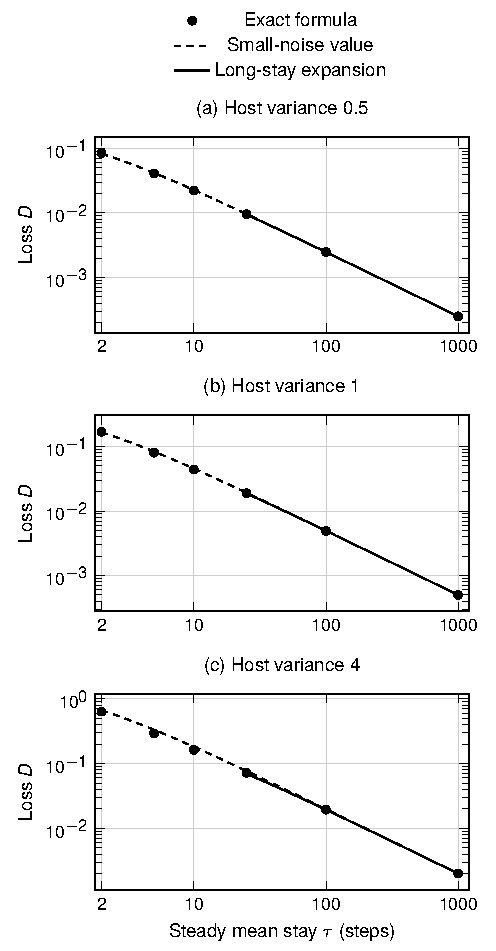
\includegraphics[width=84mm]{figures/exact-1.pdf}
\caption{Threshold loss against steady mean stay $\tau$ for illustrative host variances \textbf{(a)}~$0.5$, \textbf{(b)}~$1$, and \textbf{(c)}~$4$. Filled circles are exact-formula roots at stays $2,5,10,25,100,1000$ (validation in Online Resource~1). Dashed curves give the second-order small-noise value $Q=1/[2p(1+\tau)]$. Solid curves for $\tau\geq25$ give the two-term long-stay expansion in Proposition~\ref{prop:exact-R6}. All axes are logarithmic}\label{fig:exact-1}
\end{figure}

\subsection{Endpoint regimes and non-commuting normalized limits}\label{subsec:exact-asymptotics}

Without staying, two separate two-step cohorts each incur the full logarithmic gap $\ell(p)$. At fixed host variance, the loss approaches this endpoint at an inverse-logarithmic rate as staying tends to zero (Proposition~\ref{prop:exact-R5}, Appendix~\ref{sec:exact-app}; refereed).

The inverse-logarithmic deficit means that even very small retention reduces threshold loss (Fig.~\ref{fig:exact-2}; evaluated examples in Online Resource~1).

At long stays, the second-order approximation $Q=1/[2p(1+\tau)]$ becomes exact asymptotically at each fixed host variance (proved in Appendix~\ref{sec:exact-app}; refereed).

\begin{proposition}\label{prop:exact-R6}
Fix $p > 0$, and let $\varepsilon = 1 - s = 1/\tau$. As $\varepsilon \downarrow 0$,
\begin{equation}
\begin{split}
D(s,p) &= \frac{\varepsilon}{2p} - \frac{12p + 7}{24 p^2}\varepsilon^2 + O_p(\varepsilon^3),\\
\frac{D(s,p)}{1/[2p(1+\tau)]} &= 1 - \frac{7}{12 p \tau} + O_p(\tau^{-2}) \longrightarrow 1.
\end{split}
\label{eq:exact-long-stay}
\end{equation}
\end{proposition}

Proposition~\ref{prop:exact-R6} fixes $p$ and does not give a uniform double limit as $p\downarrow0$. Near zero staying, $Q$ understates $D$, so the small-noise expansion is not uniform in $s$ (proved in Appendix~\ref{sec:exact-app}; refereed). Numerical comparisons are in Online Resource~1.

\begin{figure}[t]
\centering
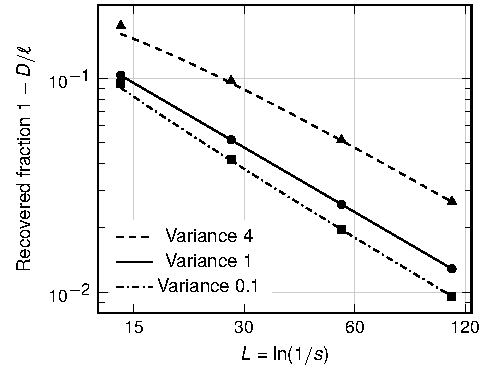
\includegraphics[width=84mm]{figures/exact-2.pdf}
\caption{Fraction of the logarithmic-gap upper bound recovered by small staying, $1 - D(s,p)/\ell(p)$, against $L = \ln(1/s)$ on logarithmic axes for illustrative host variances $1/p = 4$ ($p = 1/4$, upward triangles and dashed curve), $1/p = 1$ ($p = 1$, circles and solid curve), and $1/p = 0.1$ ($p = 10$, squares and dash-dotted curve). Markers show exact-formula evaluations at $s = 10^{-6}, 10^{-12}, 10^{-24}, 10^{-48}$ (validation in Online Resource~1), and curves show the two-term inverse-logarithm asymptotic $\psi_1(p)/(2\ell L) + \psi_1(p)[\psi(p)+\gamma]/(2\ell L^2)$ of Proposition~\ref{prop:exact-R5}, whose $L^{-2}$ term vanishes at $p = 1$}\label{fig:exact-2}
\end{figure}

Taking small noise and vanishing staying in opposite orders gives different limits after dividing loss by host variance (Proposition~\ref{prop:exact-R7}, Appendix~\ref{sec:exact-app}).

The normalized limits differ by a factor of two. Agreement with $Q$ at a fixed small stay can require very small noise (examples in Online Resource~1).

\subsection{Strict decrease of the loss with residence time at every noise level}\label{subsec:exact-theorem}

The endpoint expansions give decrease near both ends at each fixed $p$. To settle intermediate stays, we express the derivative as a covariance (proved in Appendix~\ref{sec:exact-app}; refereed).

\begin{proposition}\label{prop:exact-R4}
For $p>0$, let $T$ have density proportional to $t^{p-1}(1+t)^{-p}\mathrm{e}^{-\kappa t}$ on $t>0$, with $\kappa>0$, and put $W=\ln(1+T)$. The following parametrization covers the entire zero-growth curve $0<s<1$:
\begin{equation}
\begin{gathered}
m_p(\kappa) = \mathbb{E} W, \qquad s = \mathrm{e}^{-m_p(\kappa)},\\
V_p(\kappa) = \kappa\operatorname{Cov}(W, T) > 0,\\
g(p,\kappa) = \frac{\mathrm{d}D}{\mathrm{d}L} = \frac{1}{V_p(\kappa)} - 2 - \frac{s}{1-s},
\end{gathered}
\label{eq:exact-param}
\end{equation}
where $L=-\ln s=m_p(\kappa)$. The loss is real analytic in $s$. Its derivative is strictly negative everywhere if and only if $V_p(\kappa)<(1-s)/(2-s)$ for every $\kappa>0$.
\end{proposition}

Positivity of the covariance alone does not give the upper bound. The next theorem establishes it using a single-crossing property of the reflected density (proved in Appendix~\ref{sec:exact-app}; independently refereed as sound). Numerical evaluations illustrate the derivative but do not enter the proof.

\begin{theorem}\label{thm:exact-mono}
In the two-stage gamma model of equations~\eqref{eq:exact-matrix}--\eqref{eq:exact-defs} with $g_0, g_1 > 0$ and independent $h_t \sim \operatorname{Gamma}(p, 1/p)$, for every $p > 0$ and every $\kappa > 0$,
\begin{equation}
0 < V_p(\kappa) < \frac{1 - s}{2 - s}, \qquad s = \mathrm{e}^{-m_p(\kappa)}.
\label{eq:exact-mono}
\end{equation}
Consequently, for every $p > 0$, the threshold loss $D(s,p)$ is real analytic on $s \in (0,1)$ and satisfies $\partial_s D(s,p) < 0$ everywhere, so $D$ decreases strictly as the steady mean residence time $\tau = 1/(1-s) \in (1,\infty)$ increases. Furthermore, for each fixed $p > 0$, the logarithmic derivative $g(p,\kappa) = \mathrm{d}D/\mathrm{d}L > 0$ satisfies $\inf_{\kappa > 0} g(p,\kappa) = 0$ (unattained, with $g(p,\kappa) \sim \psi_1(p)/(2L^2) \to 0$ as $s \downarrow 0$ and $\lim_{\kappa\to\infty} g(p,\kappa) = 1/(2p)$), while for all sufficiently large $p$, $g(p,\cdot)$ has a unique local minimum on $\kappa \in [1/8, 1/2]$ at $\kappa_p = 1/4 + O(p^{-1/2})$, corresponding to $s_p = 1/(2\sqrt{p}) + O(p^{-1})$ and $g(p,\kappa_p) = 1/(8 p^{3/2}) + O(p^{-2})$.
\end{theorem}

The proof combines a strict Jensen-gap bound under integrability and single-crossing hypotheses (Proposition~\ref{prop:exact-P2}), verification for $W$ (Proposition~\ref{prop:exact-P3}), and a first-zero argument for $F=(2-s)V-(1-s)$ using the differential identities of Proposition~\ref{prop:exact-P1}. The appendix gives the full argument and endpoint expansions. The stated interior minimum is local, with no uniqueness claim outside the large-$p$ interval (Fig.~\ref{fig:exact-3}; proof outline in Online Resource~1).

\begin{figure}[t]
\centering
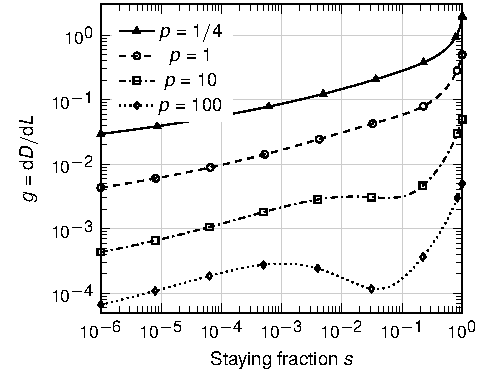
\includegraphics[width=84mm]{figures/exact-3.pdf}
\caption{Positive logarithmic derivative $g=\mathrm{d}D/\mathrm{d}L$, with $L=-\ln s$, against staying fraction $s$ for $p=1/4$ (solid, open triangles), $p=1$ (dashed, open circles), $p=10$ (dash-dotted, open squares), and $p=100$ (dotted, open diamonds). Each curve consists of 121 evaluations of the exact parametric formula in Proposition~\ref{prop:exact-R4}, with markers distinguishing the shapes. Both axes are logarithmic. The interior dips at the larger shapes do not attain the global infimum, which is zero as $s\downarrow0$}\label{fig:exact-3}
\end{figure}

\subsection{Hosts with memory}\label{subsec:exact-memory}

Host memory changes the question because the current host can be associated with the population's past stage distribution. A separate derivation, now refereed by a second independent reviewer, treats the same recurrence with a mean-one lognormal host $h_t=\exp(\sigma\xi_t-\sigma^2/2)$. Here $\xi_t$ is a centered, stationary, ergodic, unit-variance Gaussian process with covariance $\rho(j)$. For every fixed $0<s<1$, putting $q=1-s$, the derivation gives
\begin{equation}
 D=\sigma^2F_\rho(s)+O_s(\sigma^4),\qquad
 F_\rho(s)=\frac{q}{2(1+q)}
 \left[1+2\sum_{j\geq1}(-q)^{j-1}\rho(j)\right].
 \label{eq:exact-memory-coefficient}
\end{equation}
The remainder and its first $s$ derivative are uniform on compact subintervals of $0<s<1$. The series and its interior $s$ derivatives converge absolutely without covariance summability. Without ergodicity, the result concerns the zero of the expected growth exponent, not a common almost-sure threshold. The coefficient and the $2-\sqrt5$ boundary below were independently re-derived in the referee check (proofs in Appendix~\ref{subsec:exact-app-memory}). For a Gaussian first-order autoregressive process with $\rho(j)=\phi^j$, $-1<\phi<1$,
\begin{equation}
\begin{split}
 F_\phi(s)&=\frac{q[1+(q+2)\phi]}{2(1+q)(1+q\phi)},\\
 \partial_sF_\phi&=-\frac{1+2\phi+2q\phi-q^2\phi^2}
 {2(1+q)^2(1+q\phi)^2}.
\end{split}
 \label{eq:exact-memory-AR}
\end{equation}
For $2-\sqrt5\leq\phi<1$ the derivative is negative at every interior stay. For $-1/2<\phi<2-\sqrt5$ it is negative exactly when $s>1-[1-\sqrt{2(1+\phi)}]/\phi$, vanishes at that boundary, and is positive below it. For $-1<\phi\leq-1/2$ it is positive throughout.

The ring comparisons depend on which stage has staying (Proposition~\ref{prop:ring-steady}). Let $a$ and $b$ denote the fluctuating and steady mean stays. Roerdink's model has $a=1$: neither adding a steady stage with $b>1$ nor lengthening it raises the second-order loss for $0\leq\phi<1$. Proposition~\ref{prop:exact-mem-ring} in Appendix~\ref{sec:exact-app} gives the addition threshold $b<a(2a-1)\theta/(a+\theta)$, where $\theta=\phi/(1-\phi)$. With sufficiently strong positive memory, exceeding the one-stage loss requires $a>1$, whereas a rise with $b\geq1$ requires $a>(3+\sqrt{17})/4$. A third stage also permits a rise: in $(1,b,c_3)$ it occurs at short $b$ for $\phi$ near one exactly when $c_3>2$. The three-stage numerical study uses $c_3=5$ (Online Resource~1). This coefficient result does not determine every finite-amplitude curve.

The refereed derivation also proves finite-amplitude results for the bounded symmetric Markov host $h_t=1+\delta Z_t$, $0<\delta<1$, where $Z_t\in\{-1,1\}$ is stationary and $\mathbb P(Z_{t+1}=Z_t)=(1+\phi)/2$, $-1<\phi<1$. It establishes a unique invariant environment--ratio law and threshold, with $D<\ell=-\tfrac12\ln(1-\delta^2)$, and $D>0$ when $0\leq\phi<1$. At each fixed $(\delta,\phi)$, for $\varepsilon=1-s$,
\begin{equation}
 \begin{split}
 D&=A\varepsilon+B\varepsilon^2+O_{\delta,\phi}(\varepsilon^3),\\
 A&=\delta^2(1/2+\phi),\qquad
 B=-\delta^2(1/2+\phi+\phi^2)+\tfrac32A^2.
 \end{split}\label{eq:exact-memory-long}
\end{equation}
For $A\ne0$, $0<\varepsilon<|A|/262144$ ensures $\operatorname{sign}D'(s)=-\operatorname{sign}A$ and $|D'(s)+A|<|A|/2$. In particular, $\delta=1/2$, $\phi=-3/4$, and $s=1-10^{-8}$ give the proved counterexample $D'(s)>1/32$. Two deterministic methods checked the counterexamples at 80-digit working precision (details in Online Resource~1). The small-staying correction is now proved in Appendix~\ref{subsec:exact-app-memory} and checked by a second party.

For the bounded two-state host, the loss again approaches the logarithmic penalty as staying tends to zero, with a correction that depends on host memory (Proposition~\ref{prop:exact-memory-small}, Appendix~\ref{sec:exact-app}).

For the stationary gamma value-refresh kernel with $p>0$, $0\leq\phi<1$, and the lognormal autoregressive host with $\sigma>0$, $|\phi|<1$, we also prove a unique threshold, $D<\ell=-\mathbb E\ln h_t$, $D>0$ for nonnegative memory, and finite-order long-stay expansions (Appendix~\ref{subsec:exact-app-memory}, checked by a second party with the stated fixes included). The full series in $\varepsilon=1-s$ has zero radius of convergence for both hosts, so these expansions are asymptotic, not convergent.

GAP~1 is partly closed by the following result, proved in Appendix~\ref{subsec:exact-app-gap1} and checked independently.
\begin{proposition}[Uniform decrease for long stays]\label{prop:exact-memory-uniform}
For the stationary symmetric Markov host \(h_t=1+\delta Z_t\), \(Z_t\in\{-1,1\}\), with transition probabilities \(P_{ij}=(1+\phi ij)/2\), \(0<\delta<1\), and \(0\leq\phi<1\),
\begin{equation}\label{eq:exact-memory-uniform}
 D'(s)<0\qquad\text{for}\qquad 4/\sqrt{17}\leq s<1.
\end{equation}
More generally, this holds whenever \(c_*(s)/s^2\leq1/30\).
\end{proposition}
The rest of the interval, \(0<s<4/\sqrt{17}\), remains open. GAP~2 is closed and GAP~3 partly closed. For the specified unbounded hosts, memA P5's explicit derivative interval, P6's small-staying limit, and P7's noise holomorphy remain open, as does positivity for other correlated gamma kernels.

\begin{remark}[Interval certification]\label{rem:exact-certification}
GAP~4 is closed for the reported bounded-host computations, proof constants, 16 alternating-host cases, finite-state Gaussian calculations, and saved-table arithmetic, with independent checks and corrected values in Appendix~\ref{subsec:exact-app-certification}. The saved estimates classify 112 of 112 two-stage grids as decreasing and 15 of 24 three-stage grids as nonmonotone. Continuous Gaussian discretization and stochastic simulation error remain uncertified. These counts supply neither simultaneous confidence bands nor guarantees between sampled stays (Online Resource~1).
\end{remark}

\subsection{Literature status, formal verification, and biological scope}\label{subsec:exact-scope}

The literature audit distinguishes the exact solution from its threshold consequences. Roerdink's growth formula, invariant law, series, and leading small-staying growth expansion are published results \citep{roerdink1988}. The leading threshold correction and the normalized small-noise limits follow from those formulas. The audit did not find the compensated threshold analysis, strict bounds, higher small-staying corrections, long-stay expansion, or global monotonicity result in the 25 full-text documents it examined. Five target full texts, including Dyson's original, were not obtained directly. This states the scope of that search and does not establish universal priority.

Lean~4 checks the complete statements of Propositions~\ref{prop:exact-P1}, \ref{prop:exact-P2}, \ref{prop:exact-P3}, and~\ref{prop:exact-P6} under the recorded model and textbook assumptions, as well as specified components of the other exact-case results. Invariant-process and population-growth identifications and several analytic and asymptotic conclusions remain outside the credited formal coverage. The scope and remaining gaps are recorded in the reconciled coverage inventory archived with the Lean sources (see Code availability).

For a parasite with a one-step fluctuating transmission stage, independent gamma hosts, and a geometric steady stage, lengthening the steady stay strictly reduces threshold loss. The long-stay approximation holds at fixed gamma variance, with no uniform error claim as variance diverges. Host memory raises separate questions, as the bounded-host counterexample shows.

\section{Hosts with their own dynamics}\label{sec:dyn}

\paragraph{In brief.}
Once an established parasite changes host abundance, stability concerns whether small disturbances decay around an endemic equilibrium. The response of each host and parasite stage determines this local stability. When a parasite depresses a self-regulated host below the density of peak production, intermediate external-stage durations can destabilize an equilibrium that is stable at shorter and longer durations.

Once a parasite establishes in hosts that it harms, stability concerns the decay of disturbances around a positive endemic equilibrium \citep{anderson1978,dobson2020}. We analyze continuous-time hosts with births, deaths, and density dependence. The models are deterministic except in Section~\ref{subsec:dyn-noise}. An equilibrium is \emph{stable} when its Jacobian is Hurwitz (every eigenvalue has negative real part). A positive real part gives linear instability; zero or purely imaginary eigenvalues decide neither nonlinear outcome. Derivatives and gains are evaluated at equilibrium, rates have units of inverse time, and responses are dimensionless. Local symbols ($A, B, C, J, U, V_0, q, d, h, \mathcal{T}$) differ from those in Sections~\ref{sec:ring}--\ref{sec:exact}.

\subsection{Response blocks, the characteristic polynomial, and damping}\label{subsec:dyn-blocks}

A ring of $n\ge1$ blocks passes scalar infection pressure $u_k$ into block $k$ and output $v_k=u_{k+1}$ to the next block, without direct host interactions. Relative perturbations $x_k=\delta u_k/u_k^*$ and $y_k=\delta v_k/v_k^*$ satisfy $y_k(z)=E_k(z)x_k(z)$ at complex rate $z$. We retain the full internal characteristic polynomial in $E_k(z)=N_k(z)/D_k(z)$ and leave the numerator unreduced. The five blocks were derived twice and proved in Appendix~\ref{app:dyn} (Table~\ref{tab:dyn-blocks}; validation details in Online Resource 1). Block V requires $a\ge\alpha$, because parasite-killed hosts leave both $N$ and $I$.

\begin{table}[ht]
\caption{Continuous-time response blocks at a positive equilibrium ($a, c, \xi, \lambda_P > 0$, $\alpha \ge 0$)}\label{tab:dyn-blocks}
\footnotesize
\begin{tabular*}{\textwidth}{@{\extracolsep\fill}lp{0.32\textwidth}p{0.26\textwidth}p{0.25\textwidth}@{}}
\toprule
Block & \raggedright Nonlinear equations and output & \raggedright Response $E(z) = N(z)/D(z)$ & \raggedright Qualification (Prop.~\ref{prop:dyn-k3}) \tabularnewline
\midrule
L & \raggedright $\dot{w} = u - aw,\; v = cw$ & \raggedright $a/(z + a)$ & \raggedright $|E(\mathrm{i}\omega)| \le 1$; non-amplifying \tabularnewline
R$^{\mathrm{a}}$ & \raggedright $\dot{w} = u - aw,\; v = cf(w)w$ & \raggedright $(1 - \kappa)a/(z + a)$ & \raggedright Non-amp.\ $0 \le \kappa \le 2$; damping $0 < \kappa < 2$ \tabularnewline
S$^{\mathrm{b}}$ & \raggedright $\dot{I} = u(N - I) - aI,\; v = cI$ & \raggedright $a/(z + d),\; d = a/(1 - p)$ & \raggedright $|E(\mathrm{i}\omega)| \le 1 - p$; damping \tabularnewline
V$^{\mathrm{b}}$ & \raggedright $\dot{N} = \Phi(N) - \alpha I,\; v = cI,$ $\dot{I} = u(N - I) - aI$ ($a \ge \alpha$) & \raggedright $q(z + \rho)/D(z)$ ($q = a$, $d = a/(1-p)$, $h = \alpha p$) & \raggedright For $\rho \ge 0$: $|E(\mathrm{i}\omega)| \le 1 - p$; damping if $\rho + h > 0$ \tabularnewline
M$^{\mathrm{c}}$ & \raggedright $\dot{H} = \Phi(H) - \alpha P,\; v = \lambda_P P,$ $\dot{P} = uH - \xi P - \alpha\varepsilon P^2/H$ & \raggedright $q(z + \rho)/D(z)$ ($h = \alpha m$, $q = \xi + \varepsilon h$, $d = \xi + 2\varepsilon h$) & \raggedright For $\rho \ge 0$: $|E(\mathrm{i}\omega)| \le q/d$; damping if $h > 0$ \tabularnewline
\bottomrule
\end{tabular*}
\par\smallskip\noindent\footnotesize
$^{\mathrm{a}}$Evaluated with $f(w^*) > 0$ and elasticity $\kappa = -w^* f'(w^*)/f(w^*)$; $D(z) = z + a$ for L and R.
$^{\mathrm{b}}$Prevalence $p = I^*/N^* \in (0, 1)$; for V and M, $D(z) = (z + \rho)(z + d) + dh$ with $\rho = -\Phi'(X^*)$ at $X^* = N^*$ or $H^*$.
$^{\mathrm{c}}$After \citet{anderson1978}; mean burden $m = P^*/H^* > 0$, aggregation $\varepsilon \ge 1$. Exact V and M tests are in~\eqref{eq:dyn-uv}.
\end{table}

For dynamic hosts ($X = N$ or $H$), let $\rho = -\Phi'(X^*)$ and define
\begin{equation}\label{eq:dyn-abjc}
A = \rho + d, \qquad B = d(\rho + h), \qquad J = \rho + d - q, \qquad C = \rho(d - q) + dh.
\end{equation}
Equilibrium of $\dot{X}$ and differentiation of per-capita net production give
\begin{equation}\label{eq:dyn-slope}
h = \frac{\Phi(X^*)}{X^*}, \qquad \rho + h = -X^* \left.\frac{\dd}{\dd X}\frac{\Phi(X)}{X}\right|_{X = X^*}.
\end{equation}
Thus $\rho \ge 0$ means the host is held on the falling side of total net production, whereas $\rho + h > 0$ means per-capita self-regulation. Under logistic growth $\Phi(X) = rX(1 - X/K)$, a host depressed below $K/2$ has $-h < \rho < 0$, $\rho + h > 0$, and negative static response $E(0) < 0$ (over-compensation). At $\rho = -h$, per-capita production has zero local slope, with $\Phi(X) = rX$ as one example. Admissibility ($a \ge \alpha$ for V, $\varepsilon \ge 1$ for M) gives $d - q \ge h$, hence $A, J > 0$ for $\rho > -h$ and, at $\rho=-h$, $J>0$ for V, while for M, $J=(\varepsilon-1)h$ is positive exactly when $\varepsilon>1$ and $h>0$.

The full characteristic polynomial retains all disturbance modes, including those that a simplified response equation can omit (Proposition~\ref{prop:dyn-k1}, Appendix~\ref{app:dyn}).

Proposition~\ref{prop:dyn-k1} was proved in Appendix~\ref{app:dyn} and refereed. Cross-block cancellation, unobservable modes, or a zero numerator can omit roots from $\prod_kE_k(z)=1$, so the full polynomial is needed. A worked example and numerical checks are in Online Resource 1.

A block is \emph{non-amplifying} if its internal matrix is Hurwitz and $|E(\mathrm{i}\omega)| \le 1$ for all $\omega \in \mathbb{R}$, and \emph{damping} if the inequality is strict for all $\omega \in \mathbb{R}$.

\begin{theorem}[Stability of non-amplifying rings]\label{thm:dyn-k2}
If every block in a scalar-coupled ring is non-amplifying at the equilibrium and at least one block is damping, the ring is Hurwitz for any $n \ge 1$ and any positive time constants.
\end{theorem}

Theorem~\ref{thm:dyn-k2} was proved in Appendix~\ref{app:dyn} and refereed. Both hypotheses are needed: an all-L ring has a zero eigenvalue, and amplifying blocks can destabilize a ring containing a damper (example and checks in Online Resource 1).

The response criteria identify which host and parasite stages damp disturbances and which can amplify them (Proposition~\ref{prop:dyn-k3}, Appendix~\ref{app:dyn}).

Proposition~\ref{prop:dyn-k3} was proved in Appendix~\ref{app:dyn} and refereed (checks in Online Resource 1). Its qualifying rings are stable for any host count or durations. Nonnegative $\rho$ is sufficient, not necessary. For logistic production it requires $X^*\ge K/2$, which small parasite-induced mortality alone does not establish. Applications therefore require the host production curve and endemic density.

\subsection{Host depression, stage duration, and constant-number hosts}\label{subsec:dyn-delays}

Depressing a self-regulated host below peak total production ($-h < \rho < 0$) can open a bounded unstable range of external stage durations (proved in Appendix~\ref{app:dyn} and refereed).

\begin{proposition}[Self-regulated host and one delay]\label{prop:dyn-k4}
For one V block ($a_V \ge \alpha$) or M block ($\varepsilon \ge 1$) and one L block of rate $a_L > 0$ with $c_L/a_L$ and the equilibrium fixed, $\chi(z) = z^3 + (a_L + A)z^2 + (B + a_L J)z + a_L C$. When $-h < \rho < 0$, we have $A, B, C, J > 0$ and stability holds if and only if
\begin{equation}\label{eq:dyn-fquad}
F(a_L) = (a_L + A)(B + a_L J) - a_L C = J a_L^2 + (AJ + q\rho)a_L + AB > 0.
\end{equation}
Small and large $a_L$ are stable, and an open interval $a_- < a_L < a_+$ is unstable if and only if $q|\rho| - AJ > 2\sqrt{JAB}$, with
\begin{equation}\label{eq:dyn-island}
a_\pm = \frac{q|\rho| - AJ \pm \sqrt{(q|\rho| - AJ)^2 - 4JAB}}{2J},
\end{equation}
a single nonhyperbolic rate at equality, and boundary frequency $\omega^2 = B + a_L J = a_L C/(a_L + A)$.
\end{proposition}

An illustrative V host has instability for $0.0456087<a_L<1.9326281$, confirmed by stiff nonlinear integrations on both sides (Fig.~\ref{fig:dyn-1}; parameters and numerical checks in Online Resource 1).

\begin{figure}[ht]
\centering
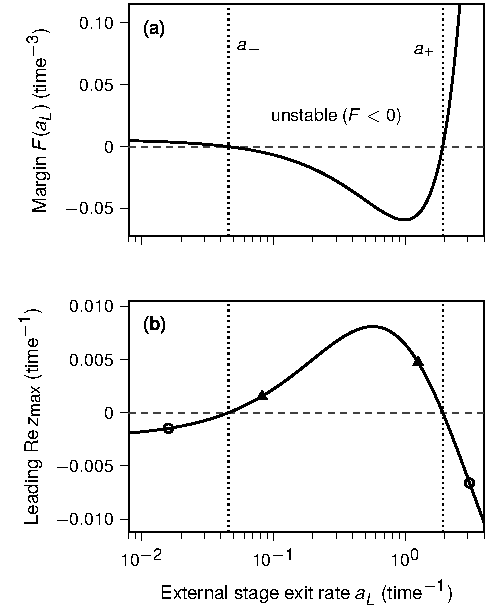
\includegraphics[width=84mm]{figures/dyn-1.pdf}
\caption{Island of instability for an illustrative depressed host ($a_V = 1.05$, $\alpha = 1$, $p = 0.20$, $h = 0.20$, $\rho = -0.196$) and one external L stage of rate $a_L$ with $c_L/a_L$ fixed. (a) Routh--Hurwitz margin $F(a_L)$ from~\eqref{eq:dyn-fquad} (solid curve), zero line (dashed), and roots $a_- = 0.0456087$, $a_+ = 1.9326281$ (dotted). (b) Leading eigenvalue real part $\operatorname{Re} z_{\max}$ (solid curve) and stiff nonlinear perturbation rates (circles for decay at $a_L = 0.0160, 3.0922$; triangles for growth at $a_L = 0.0821, 1.2562$)}\label{fig:dyn-1}
\end{figure}

For one V or M host without first-order self-regulation ($\rho=-h$, $h>0$), lengthening one external stage at fixed equilibrium and static gain cannot restore lost local stability (Proposition~\ref{prop:dyn-k5}, Appendix~\ref{app:dyn}). When the rest of the ring consists only of L stages, a chain of two stages with equal, sufficiently small exit rates is unstable for $A>0$, and every nonempty finite chain is unstable when $J\leq0$. These conclusions are restricted to rings whose remaining blocks are all L; adding damping blocks such as S can change the stability test. For one host and one L stage with fixed $d,q,h$, $d>h$, and $qd>(d-h)^2$, the lower critical rate is proportional to weak self-regulation $\delta=\rho+h$ as $\delta\downarrow0$ (the same proposition; checks in Online Resource 1).

More generally, when every other block is internally stable and its response is held fixed, write $Q(0)$ for the product of their zero-frequency responses. At fixed equilibrium and static gain, one sufficiently slow external stage stabilizes the ring if $Q(0)<1$. If $Q(0)>1$, the ring has a positive real eigenvalue at every external-stage rate; if $Q(0)=1$, it has a zero eigenvalue (Proposition~\ref{prop:dyn-k6}, Appendix~\ref{app:dyn}; refereed, checks in Online Resource 1).

One slow stage thus stabilizes even strong single-host over-compensation when the host block is internally stable ($Q(0)<0$). The appendix gives two contrasting examples: two internally stable over-compensating V blocks with $Q(0)=4$ remain unstable with one L stage, and one such V block is unstable with eight equally slow L stages. In over-compensating regulated (R/L) rings with negative total feedback and $n\geq3$, stage exit rates that are not all equal raise the critical feedback strength above its equal-rate value $\sec^n(\pi/n)$ (Proposition~\ref{prop:dyn-k7}, Appendix~\ref{app:dyn}). This criterion is published cyclic-feedback theory \citep{sontag2006,arcak2006,arcak2008,nguyen2009,hori2011,ananthasubramaniam2014} (proved in Appendix~\ref{app:dyn} and refereed; not found for parasite cycles in our search).

Constant-number hosts damp the loop, but comparisons of return speed depend on which total duration is held fixed (Proposition~\ref{prop:dyn-k8}, Appendix~\ref{app:dyn}).

\subsection{Noise response, boundary counts, and formal checks}\label{subsec:dyn-noise}

Near a Hurwitz equilibrium, transfer functions describe weak stationary infection-pressure forcing \citep[compare][]{roberts1992,marion2000}. The result was derived twice, refereed, and proved in Appendix~\ref{app:dyn}; simulation checks are in Online Resource 1.

For constant-number hosts linked by external stages, lengthening one stage at fixed equilibrium, gains, and other rates can filter weak stationary forcing along paths through it. This filtering does not remove forcing that is slow relative to both the stage and the rest of the ring's response (Proposition~\ref{prop:dyn-k9}, Appendix~\ref{app:dyn}).

This is a first-order response; no nonlinear remainder is supplied.

First Lyapunov coefficients were negative at all 900 sampled V boundaries, while M boundaries had both signs (computed once). Crossing speed and remaining eigenvalues were not checked across the sample, so these counts do not certify Hopf bifurcations. Details and nonlinear checks are in Online Resource 1.

Under their stated model and textbook assumptions, Lean~4 checks the complete statements of Proposition~\ref{prop:dyn-k1}, Theorem~\ref{thm:dyn-k2}, and Proposition~\ref{prop:dyn-k8}. For Propositions~\ref{prop:dyn-k3}, \ref{prop:dyn-k4}, and~\ref{prop:dyn-k5}, it checks every conclusion that follows from the linearized block responses, which enter the Lean files as stated rather than being derived there from the nonlinear block equations. It checks specified components of Propositions~\ref{prop:dyn-k6}, \ref{prop:dyn-k7}, and~\ref{prop:dyn-k9}. The checked declarations use no \texttt{sorry} or nonstandard axioms. Table~\ref{tab:dyn-lean} summarizes the stability results. The scope and remaining gaps are recorded in the reconciled coverage inventory archived with the Lean sources (see Code availability).

\subsection{Published grouse--nematode models and Dobson's trophic model}\label{subsec:dyn-models}

The model of \emph{Trichostrongylus tenuis} in red grouse (\emph{Lagopus lagopus scoticus}) of \citet{dobson1992} (read in full; field background \citealp{hudson1992}) and two regimes after \citet{gaba2008} fall outside the two-state V/M plus external L blocks \citep[compare][]{may1978,rosa2002}. Territorial regulation and fecundity loss affect the host response, and arrested larvae require a three-state host block. Changing durations also alters survival, $R_0$, and equilibrium host density. Additionally, host uptake directly depletes free-living larvae. Pairing the three-state response with a scalar L block reproduced the tested territorial transitions, but missed restabilization at long arrestment without territorial regulation or fecundity loss. Omitting larval-uptake saturation caused this discrepancy. These comparisons were computed once; worked examples and validation are in Online Resource 1 (Table~\ref{tab:dyn-grouse}).

Direct coupling between predator and prey hosts also breaks the scalar ring \citep{dobson1988,hadeler1989,fenton2006,rogawa2018}. Run R11 analyzed one pre-registered, dimensionally consistent reading of equations 1.6--1.11 of \citet{dobson2020} (computed once; protocol and tallies in Online Resource 1).

\begin{figure}[ht]
\centering
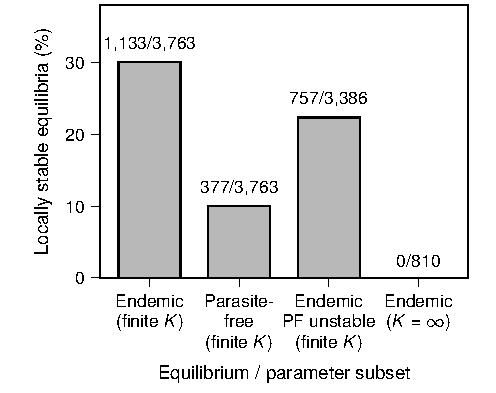
\includegraphics[width=84mm]{figures/dyn-2.pdf}
\caption{Local stability shares for the endemic system and parasite-free host subsystem in trophic sweep R11 with corrected finite-$K$ and $K = \infty$ denominators, showing endemic ($1{,}133/3{,}763 = 30.1\%$) and parasite-free host-subsystem ($377/3{,}763 = 10.0\%$) shares across finite-$K$ sets, endemic stability among host-subsystem-unstable finite-$K$ sets ($757/3{,}386 = 22.4\%$), and endemic stability for $K = \infty$ ($0/810 = 0.0\%$)}\label{fig:dyn-2}
\end{figure}

For self-limited prey, the endemic equilibrium was stable in $30.1\%$ of cases, compared with $10.0\%$ for the parasite-free subsystem (Fig.~\ref{fig:dyn-2}). None of 810 baseline endemic equilibria without prey self-limitation was stable. Longer free-living durations generally reduced stability in the tested comparisons. Stability was associated with greater relative prey density, but no threshold was established. Matched direct cycles were more often stable than trophic cycles. These are numerical findings from this sample; comparisons, uncertainty estimates, and restrictions are in Online Resource 1.

These results indicate that endemic stability depends on host production at the infected density, the location of delays, and direct predator--prey interactions. Host count and $n$th roots of $R_0$ do not determine these quantities.

%% Section 8 wrapper: pulls in the fragments as they are written.
%%   08a-computed.tex   computed studies and whole numbers
%%   08b-data.tex       what the data can and cannot test (case studies)
%%   08c-simworld.tex   the simulated world and the experiment
\section{Numerical studies, data and a simulated world}\label{sec:num}

The preceding sections prove results about a model. This section asks three further questions.
\begin{enumerate}
\item What do the results give at realistic, finite inputs?
\item What can existing data say about them?
\item Do they survive in a simulated world that relaxes the model's assumptions one at a time?
\end{enumerate}
The full studies, protocols and tables are in Online Resource~1.

% Section 8a: Computed studies
\subsection{Computed studies and whole-number populations}\label{num-computed}

To test whether the analytical results hold at realistic host-fluctuation amplitudes and non-exponential residence times, we evaluated unexpanded threshold losses and empirical stage-duration distributions numerically (Online Resource~1). Across 161 of 161 lognormal $\mathrm{AR}(1)$ ring cases (computed once), simulated loss $D$ obeyed $D \le \sum_k \sigma_k^2/2$ while exceeding $\Gamma_0$ by up to $2.14\times$ at $\sigma = 1.4$ ($3.37\times$ at $\sigma = 2.0$). Across nine illustrative literature parameterizations from separate populations (eight with one fluctuating host and one with two; \citealp{ishikawa2003,smith2007,dunn2013,anderson2015,rabone2019}), $D$ ran from $1.00\times$ to $1.63\times$ $\Gamma_0$, cutting $\sigma^2/2$ to $0.079$, $0.112$, and $0.337$ under geometric stays in \emph{Schistosoma haematobium}, \emph{S.~mansoni}, and \emph{Plasmodium falciparum}. Recomputing six complex-cycle rows across 136 regular-stay cases (computed once) preserved majority protection ($D < \sigma^2/4$ beyond three standard errors [SE]) for both schistosomes at $m = 2, 4,$ and $16$ sub-stages, failing among tested shapes at the all-fixed cycle ($D = \sigma^2/2$). In those tested schistosome families, half-protection coefficient of variation (CV) brackets were $[0, 0.043]$ on the coarse step and $[0, 0.102]$ or $[0, 0.039]$ on an $8\times$ finer step ($0.04$ is a bracket end, not an estimate), whereas \emph{P.~falciparum} failed by $m = 4$ (interpolated CVs $0.19$--$0.24$). Across 383 strict single-treatment cohorts ($n \ge 10$) from 12 of 16 open deposits (485 cohorts total), developmental clocks were tighter than survival or clearance stays (276 of 383 vs.\ 107 of 383 cohorts, median CV $0.2035$ vs.\ $0.2935$), supporting the stage-class split. Overdispersed human \emph{P.~falciparum} stays (three cohorts, CV $0.733$--$1.307$; \citealp{andrade2024}) kept one of six rows robust, while one of six was fragile in northern-edge \emph{Borrelia burgdorferi} across 35 \emph{Ixodes scapularis} cohorts \citep{brunner2022} and four of six were undecided. However, 18 of 162 uncensored cohorts ($n \ge 30$; $11.1\%$, or 21 of 165 with human malaria) failed chain representability or exceeded $10\%$ error (up to $69.6\%$) under matched-CV surrogates, contradicting CV-sufficiency because duration shape matters beyond CV.

Positive long-run growth does not prevent extinction in finite whole-number populations. Following R13's branching runs without its $10^{15}$ cap to $1{,}020{,}000$ steps ($\sigma = 0.15$, fluctuating stay $10$, $\ln R_0 = 0.0045$, computed once; threshold check at $\sigma = 0.6$) confirmed zero deaths within $6{,}000$ generations among $3{,}588$ stopped trajectories. However, 65 of 451 trajectories ($14\%$) passing $10^{15}$ at steady stay $10$ from $10{,}000$ founders later died. Under independent Poisson offspring from $10{,}000$ founders ($\phi = 0.9$), equal-step extinction rose from $0.3940 \pm 0.0109$ (no steady stage) to $0.8070 \pm 0.0088$ (stay $10$), then fell to $0.1315 \pm 0.0076$ (stay $40$) and $0.0005 \pm 0.0005$ (stay $160$), preserving 14 of 15 tested orderings (one unresolved). Grouping 100 steady parasites per host raised stay-$160$ extinction to $0.4990$ while confounding shared host death with grouped arrival. A second campaign crossed host-death hazard share $a \in \{0, 0.5, 1\}$ with packet size $K \in \{1, 10, 100\}$ across 195 cells and $365{,}000$ trajectories at matched mean matrix, reproductive value $10{,}000$, growth margin $0.005$, and $1{,}700$-step horizon (checked independently on 21 of 21 recomputed cells and 18 of 18 calibrations). Lengthening the steady stay from $10$ to $160$ lowered extinction beyond four SE in 44 of 54 like-for-like primary comparisons (by $\ge 0.01$ in 42 of 54), reversed in zero of 54, and left 10 of 54 unresolved (36 of 36 outage comparisons favored lengthening on the ten-generation clock). Shared host death ($a = 1$ vs.\ $0$) raised extinction in 12 of 54 comparisons and packet size ($K = 100$ vs.\ $1$) raised it in 36 of 54, leaving $0.1960 \pm 0.0126$ extinct at stay $160$ under mean-$200$ outages ($a = 1, K = 100$, initial burden $100$). In contrast, $D$ did not order extinction across host laws (zero of $3{,}000$ vs.\ $49$ of $1{,}000$ extinct at identical $D = 0.002144$, with 494 of $1{,}377$ equal-$D$ primary pairs differing beyond four SE). Across a zero-infection gap $G$ with independent host survival $h(G)$ and independent within-host parasite survival $p(G)$, cohort retention across $M$ hosts of burdens $b_j \ge 1$ is (proved in Online Resource~1 and checked independently)
\begin{equation}\label{num-eq-gap}
P_{\mathrm{retain}}(G) = 1 - \prod_{j=1}^{M}\Bigl\{1 - h(G)\bigl[1 - (1 - p(G))^{b_j}\bigr]\Bigr\},
\end{equation}
reaching $5\%$ retention across $100$ fresh hosts under pure host death at $7.58$ exponential mean lifetimes versus $3.48$ four-phase lifetimes.

Finally, crossing contact-limited waiting, a four-part steady stay, two equal independent alternative hosts, four asynchronous patches, and storage mortality under a bounded two-state host ($h_{\mathrm{low}} = 0.05$, variance $\mathrm{e}^{\sigma^2} - 1$) gave 192 of 320 admissible cells at two tested step sizes (checked independently on 17 of 17 recomputed cells and all counts; Section~\ref{sec:mech} and Online Resource~1). The edge bound held in 192 of 192 cells, and all 18 of 192 resolved gains involved patches. Regularizing the stay raised $D$ beyond four SE in 71 of 88 available comparisons (zero of 88 lowered, 17 of 88 unresolved), alternative hosts lowered $D$ in 73 of 96 comparisons and raised it in two of 96 (21 of 96 unresolved), and contact-limited waiting raised $D$ in 32 of 48 comparisons while lowering it in 12 of 48 without patches in the short cycle (four of 48 unresolved). Additionally, the $\sigma^2$-scaled prediction had the wrong sign in four of 192 cells (two of 192 resolved) and exceeded $30\%$ error in 160 of 192 cells (116 of 192 resolved) under this skewed host, while moderate-cycle branching extinction matched $D$'s order in 28 of 31 resolved pairs (all three of 31 reversals stemmed from one cell tilted below a tighter threshold estimate). Overall, these computations indicate that long, dispersed stays and independent host units remain protective at realistic noise amplitudes, while regular lifespans, shared host mortality, and packet transmission set demographic limits that $D$ alone does not capture.

% Section 8b: What available data can and cannot test
\subsection{What available data can and cannot test}\label{num-data}

Testing the stationary fluctuation prediction directly in empirical data requires three quantities measured together across independent populations. First, an obligate host's temporal variability (its log-abundance variance $\sigma_k^2$ and autocorrelation $\phi_k$) must vary across replicates while arithmetic-mean host abundance, mean vital rates, and background removal rates remain fixed, because changing mean host density shifts deterministic $R_0$ alongside the threshold loss $D$ (Section~\ref{sec:bounds}). Second, individual residence-time distributions must be measured for both exposed and sheltered stages rather than assumed memoryless, because stage-duration shape governs temporal averaging (Section~\ref{sec:mech}). Third, parasite persistence or rare-invasion growth must be recorded across enough generations to separate $R_0^*$ from transient carryover. However, no open dataset that we located isolates this contrast. Field surveys and museum series lack a constant-mean host control, do not measure whole-cycle $R_0$, and confound host variability with mean host abundance, alternative hosts, sampling effort, and climate. Conversely, open population and trait compilations record either host series without parasites or stage durations without longitudinal persistence outcomes. Laboratory microcosms and chemostats either hold resource inflow constant, so host crashes arise endogenously from parasite exploitation and resistance sweeps, or vary temperature or dilution in ways that simultaneously alter mean host density, washout, or parasite survival. A verification of four further candidate leads confirmed the same structural gap (Online Resource~1), because externally imposed dilution fluctuations were applied only to virus-free algal controls while zero of six ($0/6$) infected chemostats went extinct \citep{lepennec2024}, pond \textit{Daphnia magna}--\textit{Pasteuria ramosa} series came from one unmanipulated pond \citep{tadiri2026}, six-parasite \textit{D.~magna} jar experiments had neither archived trajectories nor weekly parasite censuses \citep{ebert2000}, and flour-beetle (\textit{Tribolium castaneum}) microcosm archives contained no parasite \citep{desharnais2023}.

Our initial field analyses of \textit{Borrelia burgdorferi} sensu lato in blacklegged ticks (\textit{Ixodes scapularis}) and white-footed mice (\textit{Peromyscus leucopus}) illustrate both limits. Across six Cary Institute forest plots \citep{ostfeld20182019,ostfeld2026b}, annual within-plot log-mouse SD averaged $1.030$ ($95\%$ block-bootstrap interval $[0.762, 1.217]$, $127/128$ positive plot-years, 1991--2015) by mark-recapture estimates and $0.772$ ($[0.624, 0.871]$, $191/191$ plot-years, 1991--2025) by minimum number alive, with negative annual lag-one correlations ($-0.107$ and $-0.401$), giving recomputed threshold loss $D = 0.2013 \pm 0.0002$ at $\sigma = 1.0304$ and zero memory (R12). Registered check P1 (log nymphal prevalence varying less than log mice, 1995--2013, $113/114$ nonzero plot-years) held on six of six ($6/6$) plots, and the lagged within-plot slope P2 held ($b_1 = 0.038$, $\mathrm{SE} = 0.058$, $102/104$ pairs, inside $[0, 0.587]$ at mean prevalence $0.413$) while remaining indistinguishable from zero. Both checks also held in the 2014--2022 holdout ($40/54$ plot-years with at least $20$ tested nymphs, $1{,}842/2{,}017$ ticks, B1 on $6/6$ plots, B2 $b_2 = 0.051$, $\mathrm{SE} = 0.118$, and B3 unchanged on $6/6$ plots after removing binomial variance that exceeded total variance on $2/6$ plots, R12b) \citep{ladeau2025}, although a dated correction noted that Section~\ref{sec:dyn} bounds proportional shifts in larval infection pressure rather than mouse numbers alone. Regressing August larval burdens on mouse density gave weak dilution $\kappa_2 = -0.170$ ($\mathrm{SE} = 0.100$, $107/108$ pairs, registered $-1 \le \kappa_2 \le 0$ held), whereas nymphal burden per mouse ($\kappa_1$) was unrecorded. Across $\kappa_1 \in \{0, 0.5, 1\}$ with mean-one multipliers, simulated $D$ spanned $0.0047$ to $0.1735$ at $\sigma = 1.0304$ and exceeded second-order values by $1.29\times$ to $8.41\times$ for opposite-sign sensitivities ($8/18$ cases, R12c). Across six of 13 ($6/13$) National Ecological Observatory Network (NEON) sites with at least $100$ tested \textit{I.~scapularis} nymphs ($4{,}494/4{,}591$ ticks, R14) \citep{neon2026a,neon2026b,neon2026c}, primary cross-site test T1 was not decided ($\rho = +0.4857$, exact one-sided $p = 0.8514$ negative, $p = 0.1778$ positive across $720/720$ permutations), T2 failed ($2/6$ sites above the $1.5$-site limit, $1/6$ after sampling-error adjustment), and T3 held only by its wide tolerance ($b = 0.246$, $\mathrm{SE} = 0.150$, $46/50$ pairs, inside $[0, 0.798]$). Five of the six ($5/6$) NEON sites clustered at $\sigma_{\mathrm{site}} \in [0.399, 0.571]$ against $0.989$ at Harvard Forest, and post hoc simulations ($200{,}000$ sets, between-site $\ln R_0$ SD $0.17$) using the corrected exact cutoff $\rho \le -29/35$ ($21/720$ orderings) gave only $6.8\%$ power at full proportional mouse entry against a $2.9\%$ null rate.

To examine what broader open archives can establish under pre-registered criteria, we conducted seven empirical case studies across museum specimens, population and stage-duration compilations, laboratory microcosms, and field rodent and tick surveys (Table~\ref{num-tab-casestudies}, full protocols and audit trails in Online Resource~1).

\begin{table}[htbp]
\caption{Summary of the seven pre-registered empirical case studies, their identifiable estimands, registered outcomes after second-party audit corrections, confounder controls, weather modules, and replication status}\label{num-tab-casestudies}
{\tiny\setlength{\tabcolsep}{2pt}\renewcommand{\arraystretch}{1.12}
\begin{tabular}{@{}p{0.09\textwidth}p{0.12\textwidth}p{0.11\textwidth}p{0.12\textwidth}p{0.18\textwidth}p{0.13\textwidth}p{0.08\textwidth}p{0.08\textwidth}@{}}
\toprule
System & Data & What it could identify & Registered criterion & Registered outcome (with corrections) & Main confounders and how handled & Weather included & Independent replication \\
\midrule
Puget Sound fish parasites (\texttt{wood}, 8 fish spp., 85 parasite codes) & $8{,}754$ count rows in $699$ fish, $97$ pairs, $17{,}259$ parasites, 1880--2019 ($20/85, 21/85, 44/85$ codes in $1, 2, 3+$ hosts) \citep{wood2023,wood2022} & Trait associations with temporal count slopes beyond obligate host count, not whole-cycle $R_0$ or host $\sigma^2$ & Meta ML $\Delta\mathrm{AIC}_c \le -2.0$ and bootstrap $p < 0.05$ ($B = 2{,}000$), Holm $p < 0.05$ across 4 REML traits & Not decided ($\Delta\mathrm{AIC}_c = +7.525$, $p = 0.7546$, count GLMM $\Delta\mathrm{AIC}_c = +4.315$, $0/4$ traits significant, Holm $p = 1.000$) & Unobserved hosts, guild proxies, taxonomy, dissected stage; fish and higher-taxon random effects, blind trait lock, terminal-stage check ($78/85$ taxa) & Yes (ERSSTv6 $684/699$ fish, Race Rocks $659/699$, $\Delta\mathrm{AIC}_c = +4.778$, not decided) & Reproduced$^{\mathrm{a}}$ \\
Global host series (\texttt{lpd}, birds, fish, small mammals, freshwater inverts, vectors) & $1{,}781$ series in $184$ clusters ($884$ GPDD, $887$ BioTIME, $10$ VecDyn, $N \ge 15$, after \texttt{fix1} from $1{,}842/187$) \citep{biotime2018,dornelas2018,biotime2025,dornelas2025,prendergast2010,rund2023,neon2023mosquito} & Host log-variance $\hat{\sigma}^2$, excess lag-1 memory $\Delta r_1$, and illustrative regime shares; no parasite series & T1: $M \ge 25$, $K \ge 5$, $95\%$ CI for $\Delta r_1 > 0$, median $\hat{r}_{1,\mathrm{bc}} > 0$; T2: $95\%$ lower bounds $> 20\%$ for long-cycle $>10\%$ error and $\hat{r}_{1,\mathrm{bc}} > 0.1919$ & Overall T1 supports ($\Delta r_1 = 0.348$ $[0.308, 0.391]$, median $\hat{r}_{1,\mathrm{bc}} = 0.389$) and T2 supports ($59.0\%$ $[48.0\%, 72.6\%]$, $70.3\%$ $[66.3\%, 74.8\%]$); after \texttt{fix1}, small-mammal subgroup is not decided ($34$ series, $4 < 5$ clusters; broad group $261/59$ supports) & Detrending bias (exact $\mu_0(\mathbf{t})$ subtracted), observation noise ($25\%$ check), plot pooling ($20{,}177$ series in $80$ clusters fixed-plot check), waiting death ($d = 0.125$ check) & Yes (\texttt{fix1} calendar lag: $1{,}681/1{,}781$ in $169/184$ clusters, $\Delta r_1 = 0.288$, T1/T2 support) & Reproduced$^{\mathrm{b}}$ \\
Bacteria--phage vessels (\texttt{chemostat}, \textit{Synechococcus}, \textit{E.~coli}, \textit{P.~fluorescens}) & $104$ infected and $25$ control series in $5/6$ deposits (D1 $6/3$, D2 $10/0$, D3 $22/2$, D4 $30/20$, D5 $36/0$; D6 $0$ density series) \citep{larsen2019,reuter2026,chaudhry2018,duncan2017,zhao2017} & Trajectory loss $D_{\mathrm{sim}}$, discrete edge bound (T2a), and partial association of phage density with $D_{\mathrm{sim}} \mid r_{\mathrm{const}}$ (T1) & T1: Freedman--Lane partial Spearman one-sided $p < 0.05$; T2a: discrete staying bound holds in $100\%$ of units & T2a supports ($104/104$); primary T1 not decided in $4/5$ (D1 $+0.194$, D2 $+0.028$, D3 $-0.366$ [early supports, $-0.393$, $p_- = 0.0361$], D5 $-0.179$) and contradicts in $1/5$ (D4 $+0.414$, $p_+ = 0.0147$; $30\,^{\circ}\mathrm{C}$ subset $18/30$ not decided); S2 on $H_S(t)$ flips D1 to supports ($-0.872$, $n = 6$) and D5 to contradicts ($+0.526$, $p_+ = 0.0009$, $n = 36$) & Resistance sweeps (tracked on $H_S(t)$ in S2, $25/36$ D5 extinctions), phage-driven host crashes (infected/control SD $1.71\times$--$3.51\times$), lethal $32\,^{\circ}\mathrm{C}$ arm in D4 ($6/6$ extinct, stratified in S4), fast adsorption ($5.3\%$--$13.3\%$ power) & Yes (lab chamber audit, $0$ field rows, $25$--$37\,^{\circ}\mathrm{C}$; isolates D4 $32\,^{\circ}\mathrm{C}$ lethality) & Reproduced$^{\mathrm{c}}$ \\
Microparasite microcosms and lakes (\texttt{microcosm}, phage, \textit{Holospora}, \textit{Daphnia} parasites) & $7$ open systems ($30$ phage vessels S1, $48/48$ infected/control \textit{Paramecium} metapopulations S2, $90$ tubes S3, S4--S7 incl.\ $576$ lake rows) \citep{ferris2020,duncan2013,dallas2018,dallas2016,clerc2015,tadiri2023,davenport2024,krichel2023} & Resource oscillation near 1-stage limit (T1), red vs.\ white noise and async rescue (T2), crash diagnostic (T3a) & One-sided permutation $p < 0.05$ on survival/PFU slopes (T1a,b), early $\mathrm{Red} - \mathrm{White}$ growth (T2a), day-56 prevalence (T2b), async rescue (T2c) & T1a ($\rho_S = -0.027$) and T1b ($-20.15$, $p_- = 0.259$) not decided; T2a early not decided ($-0.0074\ \mathrm{d}^{-1}$), T2b day-56 contradicts ($+0.316$, $p_+ = 0.0040$), T2c not decided ($-0.0132$ early, $-0.0632$ late); T3a $r = +0.377$ ($45/90$ tubes) diagnoses epidemic host crash & Mean-host shift under nonlinear growth ($\ln\bar{H}$ control), $5\,^{\circ}\mathrm{C}$ developmental arrest in S2 ($6/9$ Markov cells flip sign), epidemic crashes in S3, 3-day host/parasite additions in S7 & Yes (chamber audit S1--S5, S7; $576/576$ lake rows matched to 14-d Daymet/GHCN; W1a $+0.269$ not decided, W1b $0/5$ flip) & Reproduced$^{\mathrm{d}}$ \\
Mouse--tick--\textit{Borrelia} climate (\texttt{envcov}, Cary 6 grids, NEON $6/13$ sites) & $49/49$ Daymet/POWER files matched to $6/13$ NEON sites ($4{,}494$ nymphs, $46/50$ pairs) and $6$ Cary grids ($102/104$ primary, $40/54$ holdout pairs) \citep{ostfeld20182019,ladeau2025,neon2026a,neon2026b,neon2026c,thornton2022} & Climate-adjusted cross-site rank correlation (\texttt{E\_NEON\_PC1}), lagged mouse slopes (\texttt{E\_CARY\_ADJ}), thermal tick stay shifts in $D$ & Partial Spearman $p < 0.05$ ($0.05/6$ single covariates); Cary slopes compatible with $[0, 1-\bar{p}]$ within $2\,\mathrm{SE}$ & All primary tests not decided: NEON \texttt{PC1\_env} $\rho = +0.5024$ ($p_- = 0.8083$, $p_+ = 0.1931$, $6/6$ single covariates not decided), \texttt{T3\_adj} $b = 0.262$ ($\mathrm{SE} = 0.154$), Cary primary $b = 0.0366$ ($\mathrm{SE} = 0.0600$), holdout $b = 0.0502$ ($\mathrm{SE} = 0.1933$) & Trapping effort (non-confirmatory partial $\rho = +0.870$) vs.\ soil wetness ($+0.045$), Cary TFA/PCR transition ($b = 0.0843$), Wallace thermal stays ($-10.0\%$ to $+9.6\%$ same-clock $D$ shift) & Yes (6 Daymet abiotic covariates, NASA POWER, Cary ground station) & Reproduced \\
Cyclic voles and pathogens (\texttt{voles}, Kielder \textit{M.~agrestis}, Konnevesi \textit{M.~glareolus}) & 28-d step: \texttt{F02} ($1$ grid, $60$ windows, $3{,}235$ tested), \texttt{K15} ($15{,}737/17{,}883$ untreated captures, $4/7$ memory grids $N = 79$, $67$ windows), \texttt{K08} ($4$ grids, $32$--$33$ windows) \citep{paterson2022,jackson2014,voutilainen2016} & Host memory beyond $\mathrm{AR}(1)$ (\texttt{T1\_mem}), linearized K9 delayed prevalence tracking (\texttt{T2\_track}), pathogen lag order (\texttt{T3\_order}) & \texttt{T1\_mem}: $\Delta\mathrm{AIC}_c \ge +4.0$ vs.\ $\mathrm{AR}(1)$ ($\le -2.0$ contradicts); \texttt{T2\_track}: surrogate $p < 0.05$ in K9 lag window; \texttt{T3\_order}: $95\%$ CI on $\Delta L_{\mathrm{com}} > 0$ & \texttt{T1\_mem} supports on primary \texttt{F02} ($+17.390$) and pooled \texttt{K15} ($+13.321$), split on single \texttt{K15} grids ($2/4$ not decided, $2/4$ contradicts; 1-yr \texttt{K08} pooled not decided, $4/4$ single grids contradicts); \texttt{T2\_track} supports in $2/6$ series (\texttt{F02} PUUV $p = 0.0230$, lag $5$; \texttt{K08} \textit{Bartonella} $p = 0.0435$, lag $3$), not decided in $4/6$; \texttt{T3\_order} not decided in $2/2$ ($+0.282$, $+1.018$) & Antiparasitic treatments ($2{,}146/17{,}883$ excluded), Mar--Oct trapping gaps in \texttt{K15} ($11$--$17$ pairs at lags $5$--$7$), binomial variance subtraction (\texttt{D\_atten}), \texttt{SIR} cowpox serology & Registered, not executed (weather data downloaded; repeated automated failures; no weather conclusion drawn) & Not replicated$^{\mathrm{e}}$ \\
Stage-duration compilations (\texttt{devtimes}, \textit{Plasmodium}, helminths, vectors, ticks) & $383/485$ strict known-$n$ single-treatment cohorts from $12/16$ open deposits ($4/16$ had $0$ rows, $560$ exclusions) \citep{andrade2024,shapiro2017,stopard2021,fracasso2022,brunner2022,aleuy2023,johnson2023} & Individual stage $\mathrm{CV}_{\mathrm{indiv}}$ by class (\texttt{H\_dev1}), R10b row survival (\texttt{H\_sys}), two-moment CV-sufficiency (\texttt{H\_transform}) & \texttt{H\_dev1}: $95\%$ CI $\mathrm{med}(\text{dev}) < 0.50$ and $\mathrm{med}(\text{surv}) - \mathrm{med}(\text{dev}) > 0$; \texttt{H\_sys}: $D < \sigma^2/4 - 3\,\mathrm{SE}$; \texttt{H\_transform}: $\le 10\%$ error in $\ge 90\%$ of $n \ge 30$ cohorts & \texttt{H\_dev1} supports ($\text{dev}$ $0.2035$, $276/383$; $\text{surv}$ $0.2935$, $107/383$; diff $+0.0900$ $[+0.0327, +0.1545]$); \texttt{H\_sys} overall not decided ($1/6$ supports [\textit{P.~falciparum}], $1/6$ contradicts [\textit{B.~burgdorferi} north], $4/6$ not decided); \texttt{H\_transform} contradicts CV-sufficiency ($18/162 = 11.11\%$ fail $[6.79\%, 16.05\%]$; $21/165 = 12.73\%$ with malaria) & Thermal plasticity (single-$T$ cells), SE/tray-SD conflation ($420$ SE and $60$ tray rows excluded), right-censoring (Weibull MLE, $0$--$3$ skip checks), lab vs.\ field holding ($343/383$ vs.\ $40/383$) & Yes ($479/485$ cohorts with $T$, $442/485$ constant $T$; $T$ drives $\bar{t}$, $\rho = -0.943$, $R^2 = 0.0032$ on $\mathrm{CV}_{\mathrm{indiv}}$) & Not replicated$^{\mathrm{e}}$ \\
\bottomrule
\end{tabular}
\par\vspace{2pt}
$^{\mathrm{a}}$Within-$3+$ count GLMM redundant 1-level intercept removed ($\mathrm{AIC}_c$ $11{,}113.003 \to 11{,}110.989$, decision unchanged).
$^{\mathrm{b}}$BioTIME $2.0$-month seasonal cutoff and physical calendar weather lag rerun in \texttt{fix1}.
$^{\mathrm{c}}$Control $t = 0$ endpoint alignment, D2 time-weighted washout, $28/104$ nonpositive-$\phi$ $\Gamma_c$ exclusions ($76/104$ valid), and omitted D5 S2 contradicts label corrected.
$^{\mathrm{d}}$Tadiri duplicate \texttt{t56} column ($55/300$ and $77/300$ jars), unused JSON pooled SEs, and low-density denominators ($11/15$, $14/15$) corrected.
$^{\mathrm{e}}$Passed pre-analysis self-checks; not included in the five-study independent replication campaign.}
\end{table}

Overall, these seven studies show that the structural conditions analyzed in Sections~\ref{sec:ring}--\ref{sec:mech} are widespread in real host--parasite systems, while existing data do not isolate the causal persistence effect. Across open host compilations, positive temporal autocorrelation persists after removing linear trends and local weather ($\Delta r_1 = 0.288$ across $1{,}681/1{,}781$ weather-matched series), cyclic rodents require seasonal quasi-cycles beyond first-order autoregression, and observed fluctuation amplitudes push $59.0\%$ ($1{,}051/1{,}781$) of host series past a $10\%$ small-noise error on a long two-stage cycle. Similarly, measured individual stage durations depart sharply from a single geometric baseline, combining regular ectotherm development ($\text{median}\,\mathrm{CV}_{\mathrm{indiv}} = 0.2035$ across $276/383$ strict cohorts) with overdispersed human \textit{P.~falciparum} blood-stage stays ($\mathrm{CV}_{\mathrm{indiv}} = 0.733$--$1.307$) and breaking two-moment CV-sufficiency in $18/162$ ($11.11\%$) uncensored cohorts. In contrast, no study isolated exogenous host variability at a fixed mean host density with measured stage durations and persistence outcomes. Every direct empirical test of the fluctuation-loss prediction was not decided (\texttt{wood}, \texttt{envcov}, \texttt{microcosm} early invasion, and $4/5$ primary \texttt{chemostat} datasets) or contradicted where lethal heat or endogenous phage-driven host crashes and resistance sweeps reversed the association (\texttt{chemostat} D4 primary, D5 susceptible-host sensitivity, and \texttt{microcosm} day-56 \textit{Holospora} prevalence). For a parasite in nature, open observational and microcosm records therefore establish where memory, large amplitudes, waiting mortality, and return-time shape apply, and highlight the need for a controlled host-inflow experiment that holds mean host density fixed.

\subsection{Simulated populations and a controlled experiment}
\label{num-simworld}

Host fluctuations cannot be separated from changes in mean abundance, transmission,
and parasite losses in the available data. A simulated world allows these quantities
to be controlled while host variability and residence in a steady stage are changed
independently. This simulated world is theory, not evidence from nature. We use it
to examine demographic extinction and to assess what a controlled experiment would
need to measure (Online Resource 1, Section~7.8).

% Sources: virtualworld/protocol.md, report.md; verification/replication/validation-rerun.md, pilot-rerun.md.
Validation preceded the pilot. All five of five gates passed, comprising 190 of 190
registered comparisons of small-noise coefficients, mechanism extensions, the exact
gamma-host case, environmental memory, and constant-host demographic persistence.
A second party implemented separate code and repeated all 190 comparisons, with
190 of 190 passing. The full pilot was then independently repeated for 18 of 18
cells, using 400 populations per cell. These checks establish agreement with the
specified models within registered tolerances.

% Sources: virtualworld/pilot.md and its corrections; fix1-report.md; pilot-rerun-fix1.md.
The pilot crossed fixed-mean host forcing with steady mean stays of 1, 5, and
20 steps. Host variability was specified by the log-host standard deviation
($\sigma=0,0.3,0.6$) and lag-one correlation ($\phi=0,0.6$). Each of 18 cells
contained 200 independent populations, followed for 500 steps. The stationary
arithmetic mean was fixed, although individual schedules had different realized
means. The model used two geometric stages, an exposed mean stay of 2 steps,
and independent Poisson offspring at transfers. Initial abundance was 20
at $\ln R_0=0.05$ ($R_0$ is the constant-environment reproduction number),
with no host feedback. At $\phi=0.6$, the corrected noise-by-stay interaction was
$0.435$ (95\% interval $[0.321,0.549]$). This is the noise-associated increase
in extinction at stay one minus that at stay 20. The original pilot is shown
separately (Fig.~\ref{num-1}).

% Sources: verification/vworld-check/vworld-check.md; virtualworld/matched-generations-fix1.md and fix1-report.md.
However, a fixed calendar horizon gives the longer stay fewer generations of
exposure. Subtracting the constant-host controls does not remove this difference.
In the independent audit, matching reference generations reduced the interaction
to $0.22$--$0.30$, with all five of five pointwise intervals above zero.
At $\ln R_0=0.2$, the interaction was $0.49$ at 500 steps, rather than at
matched generations.
A separate corrected matched-generation run gave planning estimates of 51--61
replicate populations per cell for 80\% power, or ca.\ 244 cultures for the
core $2\times2$ comparison. These are model-conditional planning figures.
They concern marginal power at each reference horizon, not joint power
across horizons or achieved power in a biological trial.

% Sources: virtualworld/q4/report.md, including final clarification; verification/q4-check/q4-check.md; a13/report.md.
Observed host trajectories provide a different check. We replayed 120 selected
compilation series and 71 valid \textit{Tribolium} records, normalized to equal
arithmetic means. The invasion-threshold loss $D$ fell with stay in 709 of 764
adjacent comparisons. These counts include shared controls, and replay does not
establish a natural long-run process. The independent departure ledger classified
220 of 271 primary departures as explained by existing results, 51 of 271 as
requiring the hosts-with-zeros extension (A13), and zero of 271 as unresolved.
That extension now has proofs of a raw-host covariance expansion and an outage
bound under their stated conditions, with completed independent review.
The eventual derivative-sign result remains open for general unbounded hosts
with finite fourth moments. Longer stays therefore do not universally lower $D$.

% Source: notes/decisive-experiment-v2.md, especially sections 6--9 and Refereed.
A controlled experiment would compare constant and fluctuating host supply at a
fixed mean, with independently calibrated residence and survival distributions.
Held high and low densities would measure growth responses, fast and slow
switching would distinguish mean-rate changes from dynamic effects, and a period
sweep would examine sensitivity to timing. Random switching should use complete
independent mirrored pairs, with actual exposure recorded. Extinction must be
retained, and replication must include biological variation, observation error,
and uncertainty in calibrated inputs.
The earlier recommendation of one to six replicates was withdrawn after
review because it included measurement error alone. Held-density counts
also require direct infection and disappearance assays to distinguish
delayed transmission from wasted opportunities.

% Sources: notes/decisive-experiment-v2.md section 9 and Refereed; casestudies/leads/leads.md.
Candidate systems include \textit{Paramecium} with \textit{Holospora}, bacteria
with phage, and \textit{Daphnia} with \textit{Ordospora}. None is established as
feasible for this design. The \textit{Tribolium} archive already contains
fixed-mean flour fluctuations, but no parasites and no controlled equality of
beetle abundance \citep{desharnais2023}. No experiment has been run or
system selected. Density manipulation must first be separated from parasite
removal, and encounter rates, development, offspring production, and counting
must be calibrated. For a parasite, the proposed test is whether time in a
steady stage reduces the cost of variable host access once these quantities
are controlled.

\begin{figure}
\centering
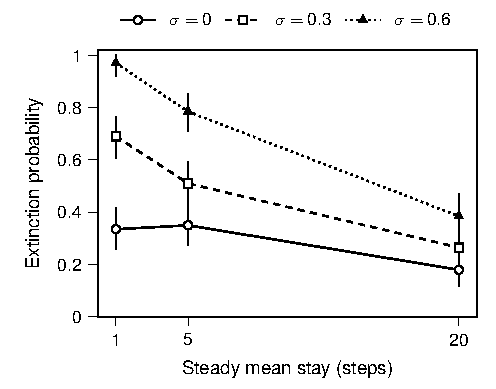
\includegraphics[width=84mm]{figures/num-1.pdf}
\caption{\textbf{Fig. X} Extinction by step 500 in the original pilot at
$\phi=0.6$. Circles with solid lines denote $\sigma=0$, squares with dashed
lines $\sigma=0.3$, and triangles with dotted lines $\sigma=0.6$.
Each point represents 200 independent populations, and bars are pointwise
95\% score intervals. Lines connect the three tested mean stays.
The exposed mean stay is 2 steps, $\ln R_0=0.05$, and initial abundance is 20.
These archived values precede the allocation correction and do not yield the
corrected interaction reported in the text. The horizon is calendar time}
\label{num-1}
\end{figure}


\section{Discussion}\label{sec:disc}

This study demonstrates that using several obligate hosts does not by itself stabilize a parasite against host fluctuations, whereas spending part of the life cycle in a stage sheltered from the fluctuating transfer does reduce the long-run growth loss under stated conditions. \citet{dobson2020} proposed that complex life cycles carry an intrinsic stability for two reasons, first because geometric averaging across $n$ hosts takes an $n$th root of the product of transmission terms, and second because long-lived stages store the parasite across another host's booms and busts. When growth is measured per unit time rather than per step of the next-generation matrix, the $n$th-root effect disappears in both deterministic regulation and stochastic persistence (Sections~\ref{sec:model} and~\ref{sec:ring}), consistent with the general equivalence of threshold criteria across life-cycle representations \citep{rueffler2013}. Adding obligate hosts in sequence without lengthening the generation time leaves two stages in one host and two hosts in series mathematically identical whenever their joint law of residence time and survival is the same (Section~\ref{sec:mech}). In contrast, the storage intuition holds as a statement about residence times. In a primitive ring with memoryless stays and scarcity that wastes failed contacts, the second-order loss in $\ln R_0$ per generation scales with log-host variance inflated by positive host memory and divided by the mean generation time $\mathcal{T}$, so a long sheltered stay drives that coefficient toward zero (Section~\ref{sec:ring}), in line with demographic buffering in structured free-living populations \citep{tuljapurkar1982a,tuljapurkar1990,morris2008,jonsson2021}. In the two-stage gamma-host model solved by \citet{roerdink1988}, we proved that this reduction holds strictly at every stay length and every noise amplitude, with the small-noise coefficient becoming asymptotically exact for long stays (Section~\ref{sec:exact}). Whether multiple hosts add buffering therefore depends on how they enter the life cycle rather than on host count alone. Obligate hosts in series do not protect by their number, whereas at fixed mean total transfer, equal shares of alternative hosts with matched log variance and memory used in parallel at one step divide that step's second-order loss by their number when their fluctuations are independent, give a weaker reduction under partial synchrony, provide no reduction in perfect synchrony, and can raise the loss when a newcomer is much noisier (Proposition~\ref{prop:ring-alt}, Section~\ref{sec:example}).

\subsection{Biological limits of stage-based buffering}\label{subsec:disc-limits}

Where that protection stops is set by life-history biology rather than mathematical technicalities (Sections~\ref{sec:mech} and~\ref{sec:num}; assumption ladder A1--A13 in Online Resource~1). First, positive host memory slows the benefit of storage and can reverse it at short durations. In a primitive two-stage geometric ring with exposed stay $a$ and steady stay $b$, adding $b \ge 1$ raises the second-order loss above the one-stage value when $a > 1$ and $b < a(2a - 1)\theta/(a + \theta)$ for memory scale $\theta = \phi/(1 - \phi)$, while lengthening $b$ can raise the coefficient under strong memory when $a > (3 + \sqrt{17})/4$ (and in a three-stage $(1, b, c_3)$ ring when $c_3 > 2$, matching nonmonotonicity in 15 of 24 finite-noise three-stage grids; Section~\ref{sec:exact}). Second, the shape of the residence-time distribution governs how lineages spread across host states \citep{tuljapurkar1990,lloyd2001}. At fixed mean generation time under positive geometric memory ($0 < \phi < 1$), greater dispersion in circuit times lowers the second-order loss through $\mathbb{E}[\phi^L]$ and can produce a net gain under heavy-tailed dormancy or relapse \citep{white2016}, whereas regular developmental clocks erode buffering until an all-fixed cycle under $n$-step ergodicity suffers the entire logarithmic-gap penalty $D = \ell$ (Section~\ref{sec:mech}). Third, survival during host scarcity and storage bounds what a long stage can save. When scarcity delays contact without waiting mortality ($d = 0$), reproductive value is conserved and $D = 0$ at every admissible amplitude, whereas waiting deaths ($0 < d \le 1$) leave a positive second-order floor $\sigma^2 d(1 - d)q_j$ even as another sheltered stay grows without bound (Proposition~\ref{prop:mech-contact}). Mortality within the sheltered stage itself taxes baseline reproduction, and in finite whole-number populations, parasites grouped in packets ($K = 100$) that share their host's death ($a = 1$) still experienced $0.1960 \pm 0.0126$ extinction at stay $160$ across mean-$200$ outages despite positive long-run growth (Section~\ref{sec:num}).

Shared or cyclic host forcing and complete host absences alter even the sign of the steady-stage effect. When a single fluctuating vector or host mediates two transfers in the loop \citep{watts2021}, or when two obligate hosts covary as predator and prey, cross-lag terms enter the second-order loss (Proposition~\ref{prop:mech-linked}). In discrete time, one host moving two unequal transfers together turns fluctuations into a second-order gain above a memory threshold (such as $\phi > 0.253$ for stays $(1, 10)$), and for linked predator--prey hosts the sequence in which the parasite uses them around the cycle changes the outcome, shifting $D$ from $+0.201$ to $-0.059 \pm 0.002$ at $\sigma = 1$ for stays $(5, 50, 5)$ (Section~\ref{sec:mech}). Similarly, when host numbers alternate or cycle in step with the parasite's generation time \citep{tuljapurkar1985,botsford2014}, resonance can make $D$ negative (Proposition~\ref{prop:ring-spectrum}), so lengthening a sheltered stage erodes a reproductive gain rather than softening a loss ($D_{\mathrm{alt}}'(s) > 0$ for $0 \le s < 1$ under period-two alternation). A parallel reversal arises when an obligate host drops to zero (assumption A13), where logarithmic moments diverge ($\ell = \infty$). Whereas persistent random outages keep $D \ge 0$ under temporal independence and leave a generally positive long-stay bound limit $-\ln[(1 - q_0)G_+]$ whenever positive host states vary, period-two boom-and-zero cycles $h = (2, 0)$ yield $D < 0$ with $D_s > 0$ at every stay, and at long stays the fourth-moment raw-covariance sum $A = \operatorname{Var}(h)/2 + \sum_{\ell \ge 1} p^{\ell - 1}\operatorname{Cov}(h_t, h_{t-\ell})$ sets the sign of $D$ and of fixed-factor stay comparisons (Section~\ref{sec:mech}). Once an established parasite depresses its hosts (Section~\ref{sec:dyn}), stability shifts again to endemic equilibrium damping \citep{anderson1978,dobson1992}, where external larval delays can destabilize weakly self-regulated hosts and none of 810 baseline trophic equilibria without prey self-limitation was stable. These boundaries are biological mechanisms of real transmission cycles, not technical caveats around a universal rule.

\subsection{Scope and asymmetry of the evidence}\label{subsec:disc-evidence}

A sharp asymmetry separates what this study establishes mathematically from what existing empirical records can decide. On the theoretical side, the analytical propositions and theorems in Sections~\ref{sec:model}--\ref{sec:dyn} rest on written proofs audited by independent second-party derivations and hostile referee checks. Across the 82 theorem, proposition, lemma, and corollary environments in the main text and appendices (25 in Sections~\ref{sec:model}--\ref{sec:dyn} and 57 in the appendices), Lean~4 checks the complete statements of nine (two in the main text), meaning every clause from the stated model, with named textbook limit theorems such as the Furstenberg--Kesten limit as explicit hypotheses. For 57 others (16 in the main text) it checks specified algebraic or analytic components, and for the remaining 16 (seven in the main text) it checks components that still carry written proof obligations. Random-matrix Lyapunov limits, stationary Markov measures, and the remaining analytic and asymptotic steps rely on the written proofs. On the simulation side, an independent implementation reproduced all 190 of 190 validation-gate comparisons across five gates and all 18 pilot cells of the demographic world, and driving that world with 120 open population series and 71 \textit{Tribolium} records traced all 271 primary departures from baseline analytical formulas without free parameters, assigning 220 to existing finite-amplitude, higher-moment, or spectral-resonance results, 51 to the absent-host extension A13, and 0 to unresolved causes (Section~\ref{sec:num}). In contrast, the data did not decide whether stage buffering stabilizes real parasites. Across seven pre-registered case studies spanning museum fish parasites, 1,781 host series, bacteria--phage vessels, microparasite microcosms and lakes, tick-borne \textit{Borrelia} surveys, cyclic voles, and 383 strict stage-duration cohorts (Table~\ref{num-tab-casestudies}), open records confirm that positive host memory, large fluctuation amplitudes, oscillatory rodent cycles, and non-exponential stage durations are realistic features of natural systems. However, none of the seven case studies drew on data that vary exogenous host fluctuations at fixed arithmetic-mean host abundance while measuring stage-duration laws and multi-generation persistence, leaving every direct empirical test undecided or confounded by mean-host shifts, thermal lethality, resistance evolution, and endogenous host crashes.

\subsection{Predictions for control, climate, and parasite decline}\label{subsec:disc-ecology}

Because the empirical studies remain inconclusive, ecological consequences of the theory must be stated as testable predictions rather than established field findings. First, for infectious disease control, we predict that pulsed vector suppression or intermittent transmission interruption at a fixed time-averaged intensity will penalize short, synchronous life cycles far more strongly than cycles anchored by long, dispersed sheltered stages \citep{smith2007,colley2014,anderson2015,gurarie2018}. In the models, multi-year adult helminths, overdispersed asymptomatic blood-stage infections \citep{andrade2020}, and relapsing liver stages \citep{white2016} absorb vector troughs, and the outage retention law in Eq.~\eqref{num-eq-gap} predicts that local elimination under buffered stages requires either maintaining zero-transmission gaps across multiple mean reservoir lifetimes or coupling vector pulses with treatment of the sheltered stage itself. Second, under climate change, we predict that complex life cycles face two interacting channels of risk \citep{morris2008,molnar2013,kutz2014,aleuy2020}. Greater rainfall and temperature variability raises host fluctuation variance $\sigma^2$ and outage frequency $q_0$, while warming accelerates ectothermic development (temperature correlated with mean stage duration at $\rho = -0.943$ across 479 cohorts in Table~\ref{num-tab-casestudies}, with $R^2 = 0.0032$ on individual CV), which shortens generation time $\mathcal{T}$ and is predicted to strip away temporal buffering unless endotherm stages supply a long, thermally insulated stay or opposing thermal slopes of mortality and development offset the loss (Proposition~\ref{prop:mech-thermal}). Third, for biodiversity loss and long-term parasite declines \citep{lafferty2009,lafferty2012,lagrue2015,wood2023}, we predict that obligate host count is a poor proxy for fluctuation risk once permanent host extirpation is separated from boom-and-bust dynamics. Instead of counting host species, field monitoring should measure sheltered and exposed stage-duration distributions, waiting-death fractions $d$ during host scarcity, directed lag covariances between predator and prey hosts, and the frequency of local host absences.

\subsection{Experimental test and open problems}\label{subsec:disc-open}

Resolving the empirical gap requires a manipulative laboratory experiment that crosses fixed-mean host supply (constant versus fluctuating host inflow at identical time-averaged host density, run in complete mirrored schedule pairs) with stage duration outside the fluctuating transfer (Section~\ref{sec:num}). In our corrected demographic simulations on matched reference-generation horizons, detecting the buffering interaction at $80\%$ power required 51--61 independent replicate populations per cell across the three valid primary horizons, or ca.\ 244 independent cultures ($61 \times 4$) for a four-cell core comparison. Candidate host--parasite systems with short generation times and free transmission stages include \textit{Paramecium caudatum} with \textit{Holospora undulata} \citep{duncan2013}, bacteria with lytic phage \citep{harrison2013}, and \textit{Daphnia} with \textit{Ordospora} \citep{krichel2023}, while parasite-free \textit{Tribolium castaneum} microcosms show that fixed-mean resource schedules can be maintained experimentally \citep{desharnais2023}. However, none of these systems is ready for an uncalibrated test because dilution or harvesting can remove free stages alongside hosts, rapid phage--bacteria runs evolve resistance, and parameter-free predictions require prior assays of encounter curvature, waiting mortality $d$, both stage-duration distributions, starting stage composition, and observation error.


\backmatter

\bmhead{Supplementary information}
Supplementary material (Online Resource~1, \texttt{ESM\_1.pdf}) is available with this preprint and in the code repository listed under Code availability.

\section*{Statements and Declarations}

\bmhead{Competing interests}
The author has no relevant financial or non-financial interests to disclose.

\bmhead{Funding}
No funding was received to assist with the preparation of this manuscript.

\bmhead{Ethics approval}
Not applicable: this theoretical and secondary-data study involved no human participants and no live animal subjects.

\bmhead{Data availability}
No new field or experimental data were collected. The Cary Institute forest-food-web dataset analysed in Section~\ref{sec:num} is publicly available on Dryad at \url{https://doi.org/10.5061/dryad.d1c8046} under a CC0~1.0 waiver \citep{ostfeld20182019}; the longer Cary Institute synthesis series is available at \url{https://doi.org/10.25390/caryinstitute.31872853.v2} under a CC~BY~4.0 licence \citep{ostfeld2026b} (see also \citealp{ostfeld2026a}, \url{https://doi.org/10.25390/caryinstitute.31915557.v1}); and the 2014--2022 Cary Institute holdout dataset is available at \url{https://doi.org/10.25390/caryinstitute.27871269.v1} under deposit metadata licence CC~BY-NC~4.0 (older embedded method notes carry a pre-publication notice, with the public deposit metadata, which give CC~BY-NC~4.0, treated as controlling in our analysis) \citep{ladeau2025}. The National Ecological Observatory Network (NEON) \texttt{RELEASE-2026} data products used in Section~\ref{sec:num} are Small mammal box trapping (\texttt{DP1.10072.001}, \url{https://doi.org/10.48443/a83h-tb34}), Tick pathogen status (\texttt{DP1.10092.001}, \url{https://doi.org/10.48443/n2yp-5a62}), and Ticks sampled using drag cloths (\texttt{DP1.10093.001}, \url{https://doi.org/10.48443/5e20-3763}), accessed 14~November 2026 \citep{neon2026a,neon2026b,neon2026c} (provisional site-months present in the downloaded bundle are not covered by the release DOIs; the DataCite records of these releases give a CC0~1.0 licence). Generated numerical results and reproduction outputs are archived at \url{https://github.com/pb-commits-it/parasite-host-fluctuations}.

\bmhead{Code availability}
All simulation, verification, Lean formalisation, and figure-generation code for this study, with the Lean coverage inventory, is archived at \url{https://github.com/pb-commits-it/parasite-host-fluctuations}.

\bmhead{Author contributions}
Paul Bergeron: conception and design of the study, direction of the analyses and verification, review and approval of the manuscript. Use of large language models in mathematical derivations, numerical and formal checks, literature searches, referee rounds, and manuscript drafting is documented in Section~\ref{sec:model}.

\bibliography{refs}

\begin{appendices}
\section{Proofs for the second-order theory of the ring}\label{app:ring}

\subsection{Further results and proofs for Section~\ref{sec:ring}}

\subsubsection{Lineage renewals, the geometric ring, the band, and serial hosts}\label{subsec:app-ring-basic}

We express the published perturbation coefficient \citep{ruelle1979,tuljapurkar1982a,tuljapurkar2006} through reproductive-value-weighted lineage return times \citep{bienvenu2015,bienvenu2017}. For a finite primitive nonnegative mean matrix $\mathbf{A}_0$, let $\lambda > 0$ be its Perron root, $\mathbf{M} = \mathbf{A}_0 / \lambda$, and $\mathbf{v}, \mathbf{w}$ its positive eigenvectors ($\mathbf{1}^{\mathsf{T}}\mathbf{v} = \mathbf{w}^{\mathsf{T}}\mathbf{v} = 1$). The probabilities $P(j \to i) = M_{ij} w_i / w_j$ define an irreducible, aperiodic Markov chain with stationary law $\pi_j = v_j w_j$.

\begin{proposition}[Lineage and renewal form]\label{prop:ring-lineage}
Under the primitive mean-matrix setting above, let $\mathbf{B} = b\mathbf{e}_i\mathbf{e}_j^{\mathsf{T}}$ ($0 < b \le M_{ij}$) be a labeled contribution to entry $(i,j)$ of $\mathbf{M}$, multiplied at step $t$ by $h(t) = \exp(z(t) - \sigma^2/2)$, where $z(t)$ is a centered stationary ergodic Gaussian series with variance $\sigma^2 > 0$ and bounded autocorrelation $\rho(\ell)$. Put $c = \mathbf{w}^{\mathsf{T}}\mathbf{B}\mathbf{v} = b w_i v_j$ (stationary use frequency) and $u(\ell) = b(\mathbf{M}^{\ell-1})_{ji}$ (reuse probability at lag $\ell \ge 1$). The formal second-order per-step cost coefficient is
\begin{equation}
C = \frac{(\mathbf{w}^{\mathsf{T}}\mathbf{B}\mathbf{v})^2}{2} - \sum_{\ell=1}^{\infty} \rho(\ell)\,\mathbf{w}^{\mathsf{T}}\mathbf{B}(\mathbf{M}^{\ell-1} - \mathbf{v}\mathbf{w}^{\mathsf{T}})\mathbf{B}\mathbf{v} = \frac{c^2}{2} - c \sum_{\ell=1}^{\infty} \rho(\ell)\,[u(\ell) - c].
\label{eq:ring-lineage}
\end{equation}
Successive uses form a renewal process with gap $L_e$ and mean $\mathcal{T}_e = \E[L_e] = 1/c$. If $\rho(\ell) = \phi^\ell$ with $|\phi| < 1$, put $\theta = \phi/(1 - \phi)$ and $R_e = \E[\phi^{L_e}]$ ($R_e = 0$ at $\phi = 0$). Then
\begin{equation}
C = \frac{1 + 2\theta}{2\mathcal{T}_e^2} - \frac{1}{\mathcal{T}_e}\frac{R_e}{1 - R_e}.
\label{eq:ring-renewal}
\end{equation}
For finitely many contributions $\mathbf{B}_a$ sharing one driver $z(t)$ with real sensitivities $\kappa_a$ via $\exp(\kappa_a z(t) - \kappa_a^2\sigma^2/2)$, summing over ordered pairs $(a,b)$ gives $C = \frac{1}{2}(\sum_a \kappa_a c_a)^2 - \sum_{a,b} \kappa_a \kappa_b c_b \sum_{\ell=1}^{\infty} \rho(\ell)\,[u_{b \to a}(\ell) - c_a]$, where $u_{b \to a}(\ell)$ is the lag-$\ell$ probability of using $a$ after $b$. Independent drivers add.
\end{proposition}

\begin{proof}[Proof of Proposition~{\upshape\ref{prop:ring-lineage}}]
Because $\mathbf{w}^{\mathsf{T}}\mathbf{M} = \mathbf{w}^{\mathsf{T}}$ and $\mathbf{w} > \mathbf{0}$, the row sums of the nonnegative probabilities $P(j \to i) = M_{ij} w_i / w_j$ satisfy $\sum_i P(j \to i) = (\sum_i M_{ij} w_i)/w_j = 1$. Primitivity of $\mathbf{A}_0$ makes $\mathbf{M}$ primitive, so the similarity transform $\mathbf{P} = \operatorname{diag}(\mathbf{w})\,\mathbf{M}\operatorname{diag}(\mathbf{w})^{-1}$ is column-stochastic, irreducible, and aperiodic. Its stationary distribution $\pi_j = v_j w_j$ satisfies $\sum_j \pi_j = \mathbf{w}^{\mathsf{T}}\mathbf{v} = 1$ and $\sum_j P(j \to i)\pi_j = \sum_j M_{ij} w_i v_j = w_i v_i = \pi_i$.

For $\mathbf{B} = b\mathbf{e}_i\mathbf{e}_j^{\mathsf{T}}$ ($0 < b \le M_{ij}$), direct multiplication gives $\mathbf{w}^{\mathsf{T}}\mathbf{B}\mathbf{v} = b w_i v_j = c$, $(\mathbf{w}^{\mathsf{T}}\mathbf{B}\mathbf{v})^2 = c^2$, and
\[
\mathbf{w}^{\mathsf{T}}\mathbf{B}\mathbf{M}^{\ell-1}\mathbf{B}\mathbf{v} = b w_i (\mathbf{M}^{\ell-1})_{ji} b v_j = c\,u(\ell), \qquad u(\ell) = b(\mathbf{M}^{\ell-1})_{ji}.
\]
Substituting these into the matrix lag sum yields Eq.~\eqref{eq:ring-lineage}. Because $\mathbf{M}$ is primitive, $\mathbf{M}^{\ell-1} - \mathbf{v}\mathbf{w}^{\mathsf{T}}$ decays geometrically in $\ell$, so the series converges absolutely whenever $\rho(\ell)$ is bounded. Under the stationary chain, state $j$ has probability $\pi_j = v_j w_j$ and chooses $\mathbf{B}$ from $j$ with probability $b w_i / w_j$, giving stationary use frequency $\pi_j b w_i / w_j = b w_i v_j = c$. Conditioned on using $\mathbf{B}$ at step $0$, the chain enters state $i$, reaches state $j$ after $\ell - 1$ steps with probability $(\mathbf{P}^{\ell-1})_{ji} = (\mathbf{M}^{\ell-1})_{ji} w_j / w_i$, and then uses $\mathbf{B}$ at step $\ell$ with probability $b w_i / w_j$, whose product is $u(\ell)$.

Because every use of $\mathbf{B}$ leaves the Markov chain in the single state $i$, the inter-use gaps $L_1, L_2, \dots$ are independent and identically distributed copies of $L_e$ with finite mean $\mathcal{T}_e = \E[L_e] = 1/c$. When $\rho(\ell) = \phi^\ell$ with $|\phi| < 1$, $|R_e| = |\E[\phi^{L_e}]| \le \E[|\phi|^{L_e}] < 1$ because $L_e \ge 1$. Since $u(\ell) = \sum_{r=1}^{\infty} \Pr(L_1 + \dots + L_r = \ell)$,
\[
\sum_{\ell=1}^{\infty} \phi^\ell u(\ell) = \sum_{r=1}^{\infty} \E\!\left[\phi^{L_1 + \dots + L_r}\right] = \sum_{r=1}^{\infty} R_e^r = \frac{R_e}{1 - R_e}, \qquad \sum_{\ell=1}^{\infty} \phi^\ell c = \frac{c\phi}{1 - \phi} = c\theta.
\]
Substituting both sums into Eq.~\eqref{eq:ring-lineage} with $c = 1/\mathcal{T}_e$ gives
\[
C = \frac{1}{2\mathcal{T}_e^2} - \frac{1}{\mathcal{T}_e}\left(\frac{R_e}{1 - R_e} - \frac{\theta}{\mathcal{T}_e}\right) = \frac{1 + 2\theta}{2\mathcal{T}_e^2} - \frac{1}{\mathcal{T}_e}\frac{R_e}{1 - R_e},
\]
which is Eq.~\eqref{eq:ring-renewal}. For several contributions $\mathbf{B}_a = b_a \mathbf{e}_{i_a}\mathbf{e}_{j_a}^{\mathsf{T}}$ sharing one driver with real sensitivities $\kappa_a$, replacing $\mathbf{B}$ by $\sum_a \kappa_a \mathbf{B}_a$ in the bilinear lag sum and using $\mathbf{w}^{\mathsf{T}}\mathbf{B}_a\mathbf{M}^{\ell-1}\mathbf{B}_b\mathbf{v} = c_b u_{b \to a}(\ell)$ and $(\mathbf{w}^{\mathsf{T}}\mathbf{B}_a\mathbf{v})(\mathbf{w}^{\mathsf{T}}\mathbf{B}_b\mathbf{v}) = c_a c_b$ gives the ordered-pair formula. Uncorrelated independent drivers have zero cross-covariances at all lags, so their coefficients add.
\end{proof}

\begin{proof}[Proof of Proposition~{\upshape\ref{prop:ring-gamma}}]
In the ring $\mathbf{A}_0$, $\mathbf{w}^{\mathsf{T}}\mathbf{A}_0 = \lambda\mathbf{w}^{\mathsf{T}}$ reads $s_k w_k + g_k w_{k+1} = \lambda w_k$ (for $n = 1$, $s_1 w_1 + g_1 w_1 = \lambda w_1$). Since $g_k > 0$ and $\mathbf{w} > \mathbf{0}$, $m_k = s_k/\lambda < 1$ and $(g_k/\lambda)(w_{k+1}/w_k) = 1 - m_k > 0$. Thus from stage $k$, the reference chain stays with probability $m_k$ and transfers to $k + 1$ with probability $1 - m_k$. Each visit to stage $k$ lasts a geometric number of steps $G_k \in \{1, 2, \dots\}$ with mean $\tau_k = (1 - m_k)^{-1} \ge 1$ and, for $0 < \phi < 1$, probability generating function
\[
\E\!\left[\phi^{G_k}\right] = \sum_{j=1}^{\infty} m_k^{j-1}(1 - m_k)\phi^j = \frac{(1 - m_k)\phi}{1 - m_k\phi} = \frac{1}{1 + \tau_k/\theta}, \qquad \theta = \frac{\phi}{1 - \phi}.
\]
Stationary transfer flux $\pi_k(1 - m_k)$ is identical across all $k$, so $\sum_{k=1}^n \pi_k = 1$ gives $\pi_k = \tau_k / \mathcal{T}$ and transfer frequency $c = \pi_k(1 - m_k) = 1/\mathcal{T}$. Between two uses of any chosen transfer, the chain visits every stage $1, \dots, n$ once in cyclic order; by the Markov property the stays $G_1, \dots, G_n$ are independent, so $L_e = \sum_{k=1}^n G_k$ has mean $\mathcal{T}$ and transform $R = \prod_{k=1}^n \E[\phi^{G_k}] = \prod_{k=1}^n (1 + \tau_k/\theta)^{-1}$ ($R = 0$ at $\phi = 0$). Applying Eq.~\eqref{eq:ring-renewal} gives $C$, and multiplying by $\mathcal{T}\sigma^2$ gives Eq.~\eqref{eq:ring-gamma}, which is symmetric in $\tau_1, \dots, \tau_n$ and independent of the chosen transfer. Additivity for independent hosts follows from Proposition~\ref{prop:ring-lineage}, and the $O(\sigma^4)$ remainder for a fixed primitive ring follows from Theorem~\ref{thm:ring-rem-ar1}.
\end{proof}

\begin{proof}[Proof of Proposition~{\upshape\ref{prop:ring-band}}]
At $\phi = 0$, $\theta = 0$ and $R = 0$, so $\Gamma = \sigma^2/(2\mathcal{T})$ equals both edges of Eq.~\eqref{eq:ring-band}. For $0 < \phi < 1$, $\theta > 0$ and $\tau_k \ge 1 > 0$, so expanding $P = \prod_{k=1}^n (1 + \tau_k/\theta)$ gives
\[
P = 1 + \sum_{k=1}^n \frac{\tau_k}{\theta} + \sum_{1 \le j < k \le n} \frac{\tau_j\tau_k}{\theta^2} + \dots \ge 1 + \frac{\mathcal{T}}{\theta},
\]
with equality if and only if $n = 1$. Since $R = 1/P \in (0, 1)$, we have $0 < R/(1 - R) = (P - 1)^{-1} \le \theta/\mathcal{T}$, with right equality if and only if $n = 1$. Subtracting $R/(1 - R)$ from $(1 + 2\theta)/(2\mathcal{T})$ yields Eq.~\eqref{eq:ring-band} and its strictness for $n \ge 2, \phi > 0$.

As $\phi \to 0^+$, $\theta \to 0$ and $R \to 0$, so $C \to 1/(2\mathcal{T}^2)$. For $\phi = \ee^{-\epsilon}$ with $\epsilon \downarrow 0$, $\theta = (\ee^\epsilon - 1)^{-1} = \epsilon^{-1} - \frac{1}{2} + O(\epsilon)$, so $(1 + 2\theta)/(2\mathcal{T}^2) = (\epsilon\mathcal{T}^2)^{-1} + O(\epsilon)$. Meanwhile $R = \E[\ee^{-\epsilon L}] = 1 - \epsilon\mathcal{T} + \frac{1}{2}\epsilon^2\E[L^2] + O(\epsilon^3)$, so
\[
\frac{1}{\mathcal{T}}\frac{R}{1 - R} = \frac{1}{\mathcal{T}}\left[\frac{1}{\epsilon\mathcal{T}}\left(1 + \frac{\epsilon\E[L^2]}{2\mathcal{T}} + O(\epsilon^2)\right) - 1\right] = \frac{1}{\epsilon\mathcal{T}^2} + \frac{\E[L^2] - 2\mathcal{T}^2}{2\mathcal{T}^3} + O(\epsilon).
\]
Subtracting gives $C = [2\mathcal{T}^2 - (\Var(L) + \mathcal{T}^2)]/(2\mathcal{T}^3) + O(\epsilon) = (1 - \mathrm{CV}^2)/(2\mathcal{T}) + O(\epsilon)$, with $\Var(L) = \sum_{k=1}^n \Var(G_k) = \sum_{k=1}^n \tau_k(\tau_k - 1)$. Finally, for fixed $n, \mathcal{T}$ and $0 < \phi < 1$, $\Gamma$ is strictly decreasing in $R$, while $-\ln R = \sum_{k=1}^n \ln(1 + \tau_k/\theta)$ is strictly concave and symmetric on the simplex $\{\tau_k \ge 1 : \sum_{k=1}^n \tau_k = \mathcal{T}\}$. By Jensen's inequality and convexity of $- \ln(1 + \tau/\theta)$, $-\ln R$ is uniquely maximized (hence $R$ minimized and $\Gamma$ maximized) at $\tau_1 = \dots = \tau_n = \mathcal{T}/n$, and minimized (hence $\Gamma$ minimized) at the vertices where $n - 1$ stays equal $1$ and one equals $\mathcal{T} - n + 1$.
\end{proof}

\begin{proof}[Proof of Proposition~{\upshape\ref{prop:ring-series}}]
Summing Eq.~\eqref{eq:ring-gamma} over $n$ independent hosts with equal $\sigma^2, \phi$ gives $\Gamma = \sigma^2 n [(1 + 2\theta)/(2\mathcal{T}) - (P - 1)^{-1}]$ (without $(P - 1)^{-1}$ at $\phi = 0$).
\begin{enumerate}
\item[(i)] Multiply Eq.~\eqref{eq:ring-band} by $n$ and substitute $\mathcal{T}/n = \bar{\tau}$.
\item[(ii)] At $\phi = 0$, $\Gamma_n = \sigma^2/(2\tau)$. For $0 < \phi < 1$, $a = 1 + \tau/\theta > 1$ and $P = a^n$. Differentiating $n/(a^n - 1)$ with respect to real $n > 0$ gives, with $x = n\ln a > 0$,
\[
\frac{\dd}{\dd n}\frac{n}{a^n - 1} = \frac{\ee^x(1 - x) - 1}{(a^n - 1)^2} < 0,
\]
because $\ee^{-x} > 1 - x$ for all $x > 0$. Thus $\Gamma_n$ strictly increases in $n$; strict decrease in $\tau$ is a special case of part~(iv).
\item[(iii)] At $\phi = 0$, $\mathcal{T} + \mathcal{T}/n = \mathcal{T}(n + 1)/n$, so $\sigma^2(n + 1)/[2\mathcal{T}(n + 1)/n] = \sigma^2 n/(2\mathcal{T})$ is unchanged. For $0 < \phi < 1$, put $x = \mathcal{T}/\theta > 0$. The new total has generation time $\mathcal{T}(1 + 1/n)$ and product $P(1 + x/n)$, so the first term $(n + 1)(1 + 2\theta)/[2\mathcal{T}(1 + 1/n)] = n(1 + 2\theta)/(2\mathcal{T})$ cancels, leaving
\[
\frac{\Delta\Gamma}{\sigma^2} = \frac{n}{P - 1} - \frac{n + 1}{P(1 + x/n) - 1} = \frac{P(x - 1) + 1}{(P - 1)[P(1 + x/n) - 1]}.
\]
Since $P > 1$, the denominator is positive. If $x \ge 1$, $P(x - 1) + 1 \ge 1 > 0$. If $0 < x < 1$, $\ln P = \sum_{k=1}^n \ln(1 + \tau_k/\theta) < \sum_{k=1}^n \tau_k/\theta = x < -\ln(1 - x)$, so $P < (1 - x)^{-1}$ and $P(x - 1) + 1 > 0$.
\item[(iv)] At $\phi = 0$, $\Gamma(c\boldsymbol{\tau}) = \sigma^2/(2c\bar{\tau})$ decreases strictly in $c$. For $0 < \phi < 1$, put $y_k = \tau_k/\theta > 0$, let $e_1, \dots, e_n$ be the elementary symmetric polynomials in $y_1, \dots, y_n$ with $e_{n+1} = 0$, and write $P(c) - 1 = D(c) = \sum_{j=1}^n e_j c^j$ and $N(c) = \sum_{i=1}^n e_{i+1} c^i$. Since $\theta/\mathcal{T} = 1/e_1$,
\[
\frac{\Gamma(c\boldsymbol{\tau})}{\sigma^2 n} = \frac{1}{2c\mathcal{T}} + \frac{1}{c e_1} - \frac{1}{D(c)} = \frac{1}{2c\mathcal{T}} + \frac{N(c)}{e_1 D(c)}.
\]
Here $(2c\mathcal{T})^{-1}$ strictly decreases in $c > 0$. Moreover,
\[
N'(c)D(c) - N(c)D'(c) = \sum_{1 \le i < j \le n} (i - j)(e_{i+1}e_j - e_{j+1}e_i)c^{i+j-1}.
\]
By Newton's inequalities, $e_i / \binom{n}{i}$ is log-concave in $i$, while $\binom{n}{i+1}/\binom{n}{i} = (n - i)/(i + 1)$ decreases in $i$, so $e_{i+1}/e_i$ is nonincreasing in $i$. Hence $e_{i+1}e_j - e_{j+1}e_i \ge 0$ and $(i - j)(e_{i+1}e_j - e_{j+1}e_i) \le 0$ for every $i < j$, so $N(c)/D(c)$ is nonincreasing in $c$.
\item[(v)] Write $A_* = (1 + 2\theta)/(2\tau^2)$ and $h = \ln a > 0$. Direct algebra gives
\begin{align*}
n(n + 1)(f_{n+1} - f_n) &= -A_* + \frac{a - 1}{\tau}\frac{n(n + 1)a^n}{(a^n - 1)(a^{n+1} - 1)} \\
&= -A_* + \frac{(a - 1)\ee^{-h/2}}{4\tau}\left[\frac{n}{\sinh(nh/2)}\right]\left[\frac{n + 1}{\sinh((n + 1)h/2)}\right].
\end{align*}
Because $u/\sinh u$ is positive and strictly decreasing for $u > 0$, $n(n + 1)(f_{n+1} - f_n)$ strictly decreases in $n$ toward $-A_* < 0$, so $f_{n+1} - f_n$ changes sign from positive to negative at most once. Consequently $\sup_{n \ge 2} f_n > f_1$ if and only if $f_2 > f_1$. Since $f_2 - f_1 = [2\theta(\tau - 1) - \tau]/[4\tau^2(2\theta + \tau)]$, this holds if and only if $\theta > \tau/[2(\tau - 1)]$. \qedhere
\end{enumerate}
\end{proof}

\subsubsection{Steady stages, alternative hosts, cyclic drivers, and continuous time}\label{subsec:app-ring-ext}

\begin{proof}[Proof of Proposition~{\upshape\ref{prop:ring-steady}}]
Each transfer in the ring has elasticity $c_k = 1/\mathcal{T}$, and an independent $\mathrm{AR}(1)$ log-host series has integrated variance $\sum_{\ell=-\infty}^{\infty} \sigma_k^2 \phi_k^{|\ell|} = \sigma_k^2(1 + 2\theta_k)$, giving leading per-step growth-variance rate $V = S_I / \mathcal{T}^2$ and per-generation rate $\mathcal{T}V = S_I / \mathcal{T}$.
\begin{enumerate}
\item[(a)] Adding stay $t > 0$ with integrated variance $s = v(1 + 2\theta_v)$ gives $(S_I + s)/(\mathcal{T} + t) < S_I / \mathcal{T}$ if and only if $s/t < S_I / \mathcal{T}$; at $v = 0$ this holds whenever $S_I > 0$.
\item[(b)] At $\phi_k = 0$, $\Gamma = S/(2\mathcal{T})$, and $(S + v)/[2(\mathcal{T} + t)] - S/(2\mathcal{T}) = (v\mathcal{T} - St)/[2\mathcal{T}(\mathcal{T} + t)]$.
\item[(c)] Setting $n = 2$, $\tau_1 = a$, $\tau_2 = b$ in Proposition~\ref{prop:ring-gamma} gives $R = \theta^2/[(\theta + a)(\theta + b)]$ and $R/(1 - R) = \theta^2/[\theta(a + b) + ab]$, proving Eq.~\eqref{eq:ring-steady}. Multiplying by $a + b$ and letting $b \to \infty$ gives $(1 + 2\theta)/2 - \theta^2/(\theta + a)$.
\item[(d)] Summing Eq.~\eqref{eq:ring-gamma} gives $\mathcal{T}V/2 - \Gamma = \sum_k \sigma_k^2 R_k/(1 - R_k) \ge 0$, and Eq.~\eqref{eq:ring-band} places $k = 2\Gamma/(\mathcal{T}V)$ in $[1/(1 + 2\theta), 1]$. For Brownian motion $B_u$ with drift $\mu > 0$ and variance $\mathcal{T}V$, $\exp(-2\mu B_u/(\mathcal{T}V))$ is a martingale, yielding $\Pr(\inf_{u \ge 0} B_u \le -x) = \exp(-Ex)$ for $x > 0$, whereas $\inf_{u \ge 0} B_u = -\infty$ almost surely for $\mu \le 0$. For one fluctuating stage $a$, $E(a) = 2a\ln R_0 / [\sigma^2(1 + 2\theta)] - 1/(1 + 2\theta)$, while for $(a,b)$, $k(a,b) = 1 - 2(a + b)\theta^2/[(1 + 2\theta)\{\theta(a + b) + ab\}]$. Direct subtraction gives
\[
E(a,b) - E(a) = \frac{2b L}{1 + 2\theta} - \left[k(a,b) - \frac{1}{1 + 2\theta}\right] = \frac{2b}{1 + 2\theta}\left[L - \frac{a\theta}{a\theta + b(a + \theta)}\right],
\]
whose bracket is negative for $L<0$ and for $L=0,\theta>0$, and is zero for $L=\theta=0$; its positive-sign condition is the one in the proposition. Because $k \in [1/(1 + 2\theta), 1]$ can increase by at most $2\theta/(1 + 2\theta)$, any stay increase $\Delta$ raises $E$ whenever $2\Delta\ln R_0 / [\sigma^2(1 + 2\theta)] > 2\theta/(1 + 2\theta)$, i.e., $\Delta\ln R_0 > \theta\sigma^2$. \qedhere
\end{enumerate}
\end{proof}

\begin{proof}[Proof of Proposition~{\upshape\ref{prop:ring-alt}} and Remark~{\upshape\ref{rem:ring-joint-stay}}]
Write the transfer contribution as $\sum_{m=1}^M \mathbf{B}_m$ with $\mathbf{B}_m = \pi_m \mathbf{B}$, so $c_m = \pi_m/\mathcal{T}$ and $u_{m' \to m}(\ell) = \pi_m u(\ell)$ where $u(\ell)$ is the single-transfer renewal probability. For independent hosts, Proposition~\ref{prop:ring-lineage} sums their individual terms with weights $\pi_m^2\sigma_m^2$, yielding Eq.~\eqref{eq:ring-alt}; Theorem~\ref{thm:ring-rem-ar1} gives the $O(\sigma^4)$ remainder because parallel contributions to one matrix entry are explicitly covered. At $\pi_1 = \pi_2 = 1/2$, $\sigma_1^2 = \sigma^2$, $\sigma_2^2 = 9\sigma^2$, and $\phi_1 = \phi_2 = \phi$, $\sum_m \pi_m^2\sigma_m^2 = (1 + 9)\sigma^2/4 = 2.5\sigma^2$. If $M$ hosts have equal shares $1/M$, common variance $\sigma^2$, common autocovariance $\gamma(\ell)$, and cross-covariance $\rho\gamma(\ell)$ for all $m \ne m'$, summing Eq.~\eqref{eq:ring-rem-lin} over the $M$ self-pairs and $M(M - 1)$ off-diagonal pairs multiplies the single-host coefficient by $[M + \rho M(M - 1)]/M^2 = [1 + \rho(M - 1)]/M$.

For a fluctuating staying contribution in stage $k$ ($m_k > 0$), $\mathbf{B} = m_k\mathbf{e}_k\mathbf{e}_k^{\mathsf{T}}$ has stationary frequency $c = \pi_k m_k = (\tau_k m_k)/\mathcal{T} = (\tau_k - 1)/\mathcal{T} = e_k$. Let $J$ be the renewal gap between successive uses of the staying edge, and put $A_* = \prod_{j \ne k} (1 + \tau_j/\theta)^{-1}$ ($\theta$ at $\psi$). Immediately after a stay in $k$, the reference chain is in stage $k$: on the next step it either stays again ($J = 1$) with probability $m_k$, or leaves $k$ with probability $1 - m_k$, traverses the remaining $n - 1$ stages with transform $A_*$, re-enters $k$, and faces the same waiting distribution $W = \E[\psi^J]$. Thus $W = m_k\psi + (1 - m_k)\psi A_* W$, giving $W = m_k\psi / [1 - (1 - m_k)\psi A_*]$. Since $R = A_* (1 - m_k)\psi / (1 - m_k\psi)$, we have
\[
\frac{W}{1 - W} = \frac{m_k\psi}{1 - m_k\psi - (1 - m_k)\psi A_*} = \frac{m_k\psi}{(1 - m_k\psi)(1 - R)}.
\]
Applying Eq.~\eqref{eq:ring-renewal} in the form $C = c^2(1 + 2\theta)/2 - c W/(1 - W)$ with $c = e_k$ yields the per-step cost and its sign criterion.

For Remark~\ref{rem:ring-joint-stay}, take $\lambda = 1$ in the two-stage ring with steady stage $0$ ($s_0 = 1 - 1/a, g_0 = 1/a$) and fluctuating-host stage $1$ ($s_1 = 1 - 1/b, g_1 = 1/b$), $\mathcal{T} = a + b$, $\mathbf{v} = (a, b)^{\mathsf{T}}/\mathcal{T}$, and $\mathbf{w} = (1, 1)^{\mathsf{T}}$. Transfer $0 \to 1$ has $\mathbf{B}_g = g_0\mathbf{e}_2\mathbf{e}_1^{\mathsf{T}}$ driven by $\xi_t$ ($\kappa_g = 1$), and staying $1 \to 1$ has $\mathbf{B}_s = s_1\mathbf{e}_2\mathbf{e}_2^{\mathsf{T}}$ driven by $\epsilon_{t+1}$ ($\kappa_s = \kappa\sqrt{1 - \phi^2}$). The self-terms in $\Gamma/\sigma^2 = \mathcal{T}C''$ are $(1 + 2\theta)/(2\mathcal{T}) - \theta^2/(\theta\mathcal{T} + ab)$ (Proposition~\ref{prop:ring-steady}(c)) and $\mathcal{T}\kappa_s^2 c_s^2/2 = \kappa^2(1 - \phi^2)(b - 1)^2/(2\mathcal{T})$ (since $\epsilon_{t+1}$ is white and $c_s = (b - 1)/\mathcal{T}$). For cross-lags, $\E[\xi_t\epsilon_{t+1}] = 0$ and $\E[\epsilon_{t+1}\xi_{t-1-m}] = 0$ for all $m \ge 0$, whereas $\E[\xi_t\epsilon_{t-m}] = \sqrt{1 - \phi^2}\,\phi^m$ for $m \ge 0$. On $\mathbf{w}^{\mathsf{T}}\mathbf{z} = 0$ (spanned by $(1, -1)^{\mathsf{T}}$), $\mathbf{T}_\perp$ acts as the scalar $s_0 + s_1 - 1 = 1 - 1/a - 1/b$. Since $\mathbf{Q}\mathbf{B}_s\mathbf{v} = s_1(b/\mathcal{T})(-a/\mathcal{T}, a/\mathcal{T})^{\mathsf{T}} = -[a(b - 1)/\mathcal{T}^2](1, -1)^{\mathsf{T}}$ and $\mathbf{w}^{\mathsf{T}}\mathbf{B}_g(1, -1)^{\mathsf{T}} = g_0 = 1/a$, the cross contribution to $C''$ in Eq.~\eqref{eq:ring-rem-lin} is
\[
-\kappa_g\kappa_s \sum_{m=0}^{\infty} \sqrt{1 - \phi^2}\,\phi^m\,\mathbf{w}^{\mathsf{T}}\mathbf{B}_g\mathbf{T}_\perp^m\mathbf{Q}\mathbf{B}_s\mathbf{v} = \frac{\kappa(1 - \phi^2)(b - 1)}{\mathcal{T}^2[1 - \phi(1 - 1/a - 1/b)]}.
\]
Multiplying by $\mathcal{T}$ gives the stated $\Gamma/\sigma^2$, whose dominant term as $b \to \infty$ at fixed $a, \phi < 1, \kappa > 0$ is $\kappa^2(1 - \phi^2)b/2$.
\end{proof}

\begin{proof}[Proof of Proposition~{\upshape\ref{prop:ring-spectrum}}]
\begin{enumerate}
\item[(a)] For any complex $|z| < 1$, $|R_e(z)| \le \E[|z|^{L_e}] < 1$, so $\sum_{\ell=1}^{\infty} z^\ell u(\ell) = R_e(z)/[1 - R_e(z)]$ and $\sum_{\ell=1}^{\infty} z^\ell c = cz/(1 - z)$. Substituting $\rho(\ell) = \sum_j B_j z_j^\ell$ into Eq.~\eqref{eq:ring-lineage} gives the finite-mixture formula. For the $\mathrm{AR}(2)$ recursion $X_t = 2r_c\cos\omega_0\,X_{t-1} - r_c^2 X_{t-2} + \eta_t$, the Yule--Walker equations give $\rho(1) = 2r_c\cos\omega_0/(1 + r_c^2)$ and $\rho(\ell) = \operatorname{Re}(B z^\ell) = \frac{1}{2}B z^\ell + \frac{1}{2}\bar{B}\bar{z}^\ell$ for $\ell \ge 0$ with $z = r_c\ee^{\mathrm{i}\omega_0}$ and $B = 1 + \mathrm{i}[\cos\omega_0 - \rho(1)/r_c]/\sin\omega_0$.
\item[(b)] Because $\mathbf{M}$ is primitive and $b > 0$, $u(\ell) > 0$ for all sufficiently large $\ell$, so the support of $L_e$ has greatest common divisor $1$ and $g(\omega) = \E[\ee^{\mathrm{i}\omega L_e}] \ne 1$ for every $\omega \in (0, 2\pi)$. For $|\zeta| < 1$, write $F(\zeta) = \E[\zeta^{L_e}]$ and decompose
\[
\sum_{\ell=1}^{\infty} [u(\ell) - c]\zeta^\ell + \frac{c\zeta}{1 - \zeta} = \frac{F(\zeta)}{1 - F(\zeta)}.
\]
Since $|u(\ell) - c|$ decays geometrically, the first series converges uniformly on $|\zeta| \le 1$. Letting $\zeta = r\ee^{\mathrm{i}\omega}$ with $r \uparrow 1$ for $\omega \in (0, \pi]$ and taking real parts (using $\operatorname{Re}[\ee^{\mathrm{i}\omega}/(1 - \ee^{\mathrm{i}\omega})] = -1/2$) gives
\[
\sum_{\ell=1}^{\infty} [u(\ell) - c]\cos(\omega\ell) = \operatorname{Re}\frac{g(\omega)}{1 - g(\omega)} + \frac{c}{2},
\]
which extends continuously to $\omega = 0$. Substituting $\rho(\ell) = \pi^{-1}\int_0^\pi f(\omega)\cos(\omega\ell)\dd\omega$ into Eq.~\eqref{eq:ring-lineage} and exchanging the finite integral with the geometrically convergent sum yields
\[
c\sum_{\ell=1}^{\infty} \rho(\ell)[u(\ell) - c] = \frac{c}{\pi}\int_0^\pi f(\omega)\operatorname{Re}\frac{g(\omega)}{1 - g(\omega)}\dd\omega + \frac{c^2}{2}\cdot\frac{1}{\pi}\int_0^\pi f(\omega)\dd\omega.
\]
Since $\pi^{-1}\int_0^\pi f(\omega)\dd\omega = 1$ and $c = 1/\mathcal{T}_e$, the $c^2/2$ term cancels that of Eq.~\eqref{eq:ring-lineage}, proving Eq.~\eqref{eq:ring-spectrum}.
\item[(c)] Taking white noise $f(\omega) \equiv 1$ ($\rho(\ell) = 0$ for $\ell \ge 1$) gives $\pi^{-1}\int_0^\pi K(\omega)\dd\omega = C_{\mathrm{white}} = c^2/2 = 1/(2\mathcal{T}_e^2)$. As $\omega \to 0$, $g(\omega) = 1 + \mathrm{i}\omega\mathcal{T}_e - \frac{1}{2}\omega^2\E[L_e^2] + O(\omega^3)$, so
\[
\begin{aligned}
1 - g(\omega) &= -\mathrm{i}\omega\mathcal{T}_e\left(1 + \frac{\mathrm{i}\omega\E[L_e^2]}{2\mathcal{T}_e} + O(\omega^2)\right), \\
\operatorname{Re}\frac{g(\omega)}{1 - g(\omega)} &= \operatorname{Re}\left(\frac{1}{1 - g(\omega)} - 1\right) \to \frac{\E[L_e^2]}{2\mathcal{T}_e^2} - 1 = \frac{\mathrm{CV}^2 - 1}{2},
\end{aligned}
\]
giving $K(\omega) \to (1 - \mathrm{CV}^2)/(2\mathcal{T}_e)$. For a one-stage transfer, $g(\omega) = (1 - m)\ee^{\mathrm{i}\omega}/(1 - m\ee^{\mathrm{i}\omega})$, so $g(\omega)/[1 - g(\omega)] = (1 - m)\ee^{\mathrm{i}\omega}/(1 - \ee^{\mathrm{i}\omega})$, whose real part is $-(1 - m)/2 = -1/(2\tau)$, giving $K(\omega) = 1/(2\tau^2)$. For $n \ge 2$ in a primitive ring, $(1 - \mathrm{CV}^2)/(2\mathcal{T}) > 1/(2\mathcal{T}^2)$ is equivalent to $\mathcal{T}^2 - \Var(L) > \mathcal{T}$, which holds because $\mathcal{T}^2 - \sum_{k=1}^n \tau_k(\tau_k - 1) - \mathcal{T} = 2\sum_{1 \le j < k \le n} \tau_j\tau_k > 0$. Finally, $\operatorname{Re}[g/(1 - g)] = (\operatorname{Re} g - |g|^2)/|1 - g|^2$ makes $K(\omega) < 0$ if and only if $\operatorname{Re} g(\omega) > |g(\omega)|^2$, and the eight-stage example in the main text shows non-monotonicity. \qedhere
\end{enumerate}
\end{proof}

\begin{proposition}[Continuous-time ring]\label{prop:ring-ct}
In $\dd x_{k+1}/\dd t = b_k\nu_k h_k(t) x_k - (\nu_{k+1} + \mu_{k+1}) x_{k+1}$ ($k$ modulo $n$, $b_k\nu_k > 0$, fixed $\nu_k + \mu_k > 0$, baseline growth $r_0$), set $a_k = r_0 + \nu_k + \mu_k > 0$, $T = \sum_{k=1}^n 1/a_k$, and $R = \prod_{k=1}^n a_k/(a_k + \alpha)$ ($\alpha > 0$).
\begin{enumerate}
\item[(a)] With independent Ornstein--Uhlenbeck drivers $z_k$ ($\Cov[z_k(t), z_k(0)] = \ee^{-\alpha|t|}$) in $h_k = \exp(\sigma z_k - \sigma^2/2)$, each exposed transfer has formal second-order cost
\begin{equation}
\sigma^2\left[\frac{1}{\alpha T^2} - \frac{1}{T}\frac{R}{1 - R}\right] \ \text{per unit time}, \qquad \Gamma = \sigma^2\left[\frac{1}{\alpha T} - \frac{R}{1 - R}\right] \ \text{per generation}.
\label{eq:ring-ct}
\end{equation}
For $n = 1$ the cost is zero at every $\sigma$; for $n \ge 2$ the per-time coefficient lies in $(0, (\alpha T^2)^{-1})$. At equal $a_k = q$ across $n$ fluctuating hosts, $\sigma^2[q/\alpha - n/\{(1 + \alpha/q)^n - 1\}]$ strictly increases with $n$ (limits $\sigma^2(n - 1)/2$ as $\alpha \to 0$ and $\sigma^2 q/\alpha$ as $\alpha \to \infty$, $n \ge 2$), while unequal stays can lower the total ($\sigma^2/3$ for $(1,1)$ versus $0.022\sigma^2$ for $(1,1,100)$ at $\alpha = 1$).
\item[(b)] With fixed gains and net stage-$j$ loss rate $\bar{\mu}_j + \sigma z(t)$ (or $\bar{\mu}_j\exp(\epsilon z - \epsilon^2/2)$ with $\bar{\mu}_j^2\epsilon^2$ for $\sigma^2$), put $p_j = 1/(a_j T)$. The formal per-time cost $\sigma^2 p_j [p_j/\alpha - \{(a_j + \alpha)(1 - R)\}^{-1}]$ is zero for $n = 1$ and negative for $n \ge 2$, with fast limit $-\sigma^2 p_j(1 - p_j)/\alpha$ \citep{monmarche2025}.
\end{enumerate}
\end{proposition}

\begin{proof}[Proof of Proposition~{\upshape\ref{prop:ring-ct}}]
\begin{enumerate}
\item[(a)] Let $\mathbf{A}_0$ be the mean generator with Perron eigenvalue $r_0$ and positive eigenvectors $\mathbf{v}, \mathbf{w}$ ($\mathbf{w}^{\mathsf{T}}\mathbf{v} = 1$), and set $\mathbf{H} = \mathbf{A}_0 - r_0\mathbf{I}$ and $\mathbf{Q} = \mathbf{I} - \mathbf{v}\mathbf{w}^{\mathsf{T}}$. For one fluctuating gain $\mathbf{B} = b_k\nu_k\mathbf{e}_{k+1}\mathbf{e}_k^{\mathsf{T}}$ with $h_k(t) = \exp(\sigma z_k(t) - \sigma^2/2) = 1 + \sigma z_k(t) + \frac{1}{2}\sigma^2(z_k(t)^2 - 1) + O(\sigma^3)$, normalize $\mathbf{y}(t) = \mathbf{x}(t)/(\mathbf{w}^{\mathsf{T}}\mathbf{x}(t))$, so $\dd\ln(\mathbf{w}^{\mathsf{T}}\mathbf{x})/\dd t = \mathbf{w}^{\mathsf{T}}\mathbf{A}(t)\mathbf{y}(t) = r_0 + (h_k(t) - 1)\mathbf{w}^{\mathsf{T}}\mathbf{B}\mathbf{y}(t)$. Expanding $\mathbf{y}(t) = \mathbf{v} + \sigma\mathbf{y}_1(t) + O(\sigma^2)$ with $\mathbf{w}^{\mathsf{T}}\mathbf{y}_1 = 0$ gives $\dd\mathbf{y}_1/\dd t = \mathbf{H}\mathbf{y}_1 + z_k(t)\mathbf{Q}\mathbf{B}\mathbf{v}$, whose stationary solution is $\mathbf{y}_1(t) = \int_0^{\infty} \ee^{\mathbf{H}s}\mathbf{Q}\mathbf{B}\mathbf{v}\,z_k(t - s)\dd s$. Taking expectations with $\E[z_k(t)^2 - 1] = 0$ and $\E[z_k(t)z_k(t - s)] = \ee^{-\alpha s}$ gives second-order growth gain $\sigma^2\int_0^{\infty} \ee^{-\alpha s}\mathbf{w}^{\mathsf{T}}\mathbf{B}\ee^{\mathbf{H}s}\mathbf{Q}\mathbf{B}\mathbf{v}\dd s = \sigma^2\mathbf{w}^{\mathsf{T}}\mathbf{B}(\alpha\mathbf{I} - \mathbf{H})^{-1}\mathbf{Q}\mathbf{B}\mathbf{v}$. Under the lineage generator $\operatorname{diag}(\mathbf{w})\,\mathbf{H}\operatorname{diag}(\mathbf{w})^{-1}$, stage $j$ exits to $j + 1$ at rate $a_j = r_0 + \nu_j + \mu_j$, so stationary flux is $c = \mathbf{w}^{\mathsf{T}}\mathbf{B}\mathbf{v} = 1/T$, the circuit Laplace transform is $R = \prod_{j=1}^n a_j/(a_j + \alpha)$, continuous-time renewal gives $\mathbf{w}^{\mathsf{T}}\mathbf{B}(\alpha\mathbf{I} - \mathbf{H})^{-1}\mathbf{B}\mathbf{v} = c R/(1 - R)$, and the Perron part is $c^2/\alpha = 1/(\alpha T^2)$. Subtracting the gain from zero gives Eq.~\eqref{eq:ring-ct}. Equivalently, setting $1 - m_j = a_j\Delta$ and $\phi = \ee^{-\alpha\Delta}$ in Proposition~\ref{prop:ring-gamma}, dividing the per-step cost by $\Delta$, and letting $\Delta \downarrow 0$ yields the same expression.

For $n = 1$, $\dd x_1/\dd t = [b_1\nu_1 h_1(t) - (\nu_1 + \mu_1)]x_1$, so $t^{-1}\ln x_1(t) \to b_1\nu_1\E h_1 - (\nu_1 + \mu_1) = r_0$ at every $\sigma$ because $\E h_1 = 1$ (and $R/(1 - R) = a_1/\alpha = 1/(\alpha T)$). For $n \ge 2$, $\prod_{j=1}^n (1 + \alpha/a_j) - 1 > \alpha\sum_{j=1}^n 1/a_j = \alpha T$, so $0 < R/(1 - R) < 1/(\alpha T)$ and the cost coefficient lies strictly in $(0, (\alpha T^2)^{-1})$. At equal $a_j = q$ across $n$ hosts, $T = n/q$ and $R = (1 + \alpha/q)^{-n}$, giving $\sigma^2[q/\alpha - n/\{(1 + \alpha/q)^n - 1\}]$, which strictly increases in $n$ as in Proposition~\ref{prop:ring-series}(ii); expanding in $\alpha \to 0$ gives $\sigma^2(1 - \mathrm{CV}^2)/2 = \sigma^2(1 - 1/n)/2$ per host, so $\sigma^2(n - 1)/2$ in total, while $\alpha \to \infty$ gives $\sigma^2 q/\alpha$ for $n \ge 2$.
\item[(b)] For net loss rate $\bar{\mu}_j + \sigma z(t)$, set $\mathbf{B} = -\mathbf{e}_j\mathbf{e}_j^{\mathsf{T}}$; the direct second-derivative expectation vanishes (and likewise for $\bar{\mu}_j\exp(\epsilon z - \epsilon^2/2)$, where $\E[\ee^{\epsilon z - \epsilon^2/2} - 1] = 0$ to all orders). Thus the per-time cost coefficient per $\sigma^2$ is $-\mathbf{w}^{\mathsf{T}}\mathbf{B}(\alpha\mathbf{I} - \mathbf{H})^{-1}\mathbf{Q}\mathbf{B}\mathbf{v}$, with $\mathbf{w}^{\mathsf{T}}\mathbf{B}\mathbf{v} = -\pi_j = -1/(a_j T) = -p_j$. Because the lineage stays in $j$ for an exponential time of rate $a_j$ or returns after any number of circuits of Laplace transform $R$, the $(j,j)$ entry of $(\alpha\mathbf{I} - \mathbf{H})^{-1}$ is $[(a_j + \alpha)(1 - R)]^{-1}$, giving $\sigma^2 p_j [p_j/\alpha - \{(a_j + \alpha)(1 - R)\}^{-1}]$. Put $x_k = \alpha/a_k > 0$. For $n = 1$, $p_1 = 1$ and $1 - R = \alpha/(a_1 + \alpha)$, giving zero. For $n \ge 2$, negativity $p_j/\alpha < [(a_j + \alpha)(1 - R)]^{-1}$ reduces, upon substituting $p_j = x_j/(\sum_k x_k)$ and $1 - R = 1 - (1 + x_j)^{-1}\prod_{k \ne j}(1 + x_k)^{-1}$, to
\[
1 - \prod_{k \ne j} \frac{1}{1 + x_k} < \sum_{k \ne j} x_k.
\]
Putting $y_k = x_k/(1 + x_k) \in (0, 1)$, we have $1 - \prod_{k \ne j}(1 - y_k) \le \sum_{k \ne j} y_k < \sum_{k \ne j} x_k$, which is strict whenever $\{k \ne j\}$ is nonempty. As $\alpha \to \infty$, $R \to 0$ and $(a_j + \alpha)^{-1} = \alpha^{-1} + O(\alpha^{-2})$, giving $-\sigma^2 p_j(1 - p_j)/\alpha$. \qedhere
\end{enumerate}
\end{proof}

\subsubsection{Proofs of the remainder theorems}\label{subsec:app-ring-rem}

\begin{theorem}[$\mathrm{AR}(1)$ remainder]\label{thm:ring-rem-ar1}
Fix dimension $d \ge 1$ and finitely many labeled contributions $a$ in $\mathbf{A}(t) = \mathbf{A}_{\mathrm{fixed}} + \sum_a a_a h_a(t)\,\mathbf{e}_{i_a}\mathbf{e}_{j_a}^{\mathsf{T}}$ with $\mathbf{A}_{\mathrm{fixed}} \ge \mathbf{0}$, $a_a > 0$, $\kappa_a \in \mathbb{R}$, primitive $\mathbf{A}_0 = \mathbf{A}_{\mathrm{fixed}} + \sum_a a_a\mathbf{e}_{i_a}\mathbf{e}_{j_a}^{\mathsf{T}}$ ($\mathbf{1}^{\mathsf{T}}\mathbf{v} = \mathbf{w}^{\mathsf{T}}\mathbf{v} = 1$), and $h_a(t) = \exp(\sigma\kappa_a\xi_{\delta(a)}(t) - \sigma^2\kappa_a^2/2)$ driven by independent stationary unit-variance Gaussian $\mathrm{AR}(1)$ series $\xi_\delta$ ($|\phi_\delta| < 1$). Put $\mathbf{M} = \mathbf{A}_0/\lambda$, $\mathbf{Q} = \mathbf{I} - \mathbf{v}\mathbf{w}^{\mathsf{T}}$, $\mathbf{T}_\perp = \mathbf{M} - \mathbf{v}\mathbf{w}^{\mathsf{T}}$, $\mathbf{B}_a = (a_a/\lambda)\mathbf{e}_{i_a}\mathbf{e}_{j_a}^{\mathsf{T}}$, and $c_a = \mathbf{w}^{\mathsf{T}}\mathbf{B}_a\mathbf{v}$. From $\mathbf{x}(0) = \mathbf{v}$ with stationary noise, $r(\sigma) = \lim_{N \to \infty} N^{-1}\E\ln(\mathbf{1}^{\mathsf{T}}\mathbf{x}(N))$ exists, and for model-dependent $\sigma_0 > 0, K < \infty$,
\begin{equation}
\begin{aligned}
\bigl|\ln\lambda - r(\sigma) - C\sigma^2\bigr| &\le K\sigma^4 \quad (|\sigma| \le \sigma_0), \\
C &= \sum_{\substack{a,b\\ \delta(a)=\delta(b)}} \kappa_a\kappa_b \left[ \frac{c_a c_b}{2} - \phi_{\delta(a)}\,\mathbf{w}^{\mathsf{T}}\mathbf{B}_a(\mathbf{I} - \phi_{\delta(a)}\mathbf{T}_\perp)^{-1}\mathbf{Q}\mathbf{B}_b\mathbf{v} \right].
\end{aligned}
\label{eq:ring-rem-ar1}
\end{equation}
\end{theorem}

\begin{proof}[Proof of Theorem~{\upshape\ref{thm:ring-rem-ar1}}]
If every $\kappa_a = 0$ (or the contribution list is empty), $\mathbf{A}(t) \equiv \mathbf{A}_0$ and $\ln\lambda - r(\sigma) = C = 0$ identically. Otherwise fix the model and normalize the state by $\mathbf{y}(t) = \mathbf{x}(t)/(\mathbf{w}^{\mathsf{T}}\mathbf{x}(t))$ in $\Delta_w = \{\mathbf{y} \ge \mathbf{0} : \mathbf{w}^{\mathsf{T}}\mathbf{y} = 1\}$, starting at $\mathbf{y}(0) = \mathbf{v}$. On $\Delta_w$, Euclidean norms satisfy $|\mathbf{y}| \le 1/w_{\min}$ where $w_{\min} = \min_i w_i > 0$. Put $G_t = \mathbf{w}^{\mathsf{T}}\mathbf{A}(t)\mathbf{y}(t) > 0$, so $\mathbf{y}(t + 1) = \mathbf{A}(t)\mathbf{y}(t)/G_t$ and $\ln(\mathbf{w}^{\mathsf{T}}\mathbf{x}(N)) = \sum_{t=0}^{N-1} \ln G_t$. Let $V_0 = \{\mathbf{z} \in \mathbb{R}^d : \mathbf{w}^{\mathsf{T}}\mathbf{z} = 0\}$, which is invariant under $\mathbf{M}$ because $\mathbf{w}^{\mathsf{T}}\mathbf{M} = \mathbf{w}^{\mathsf{T}}$. For every fixed noise path, $h_a(t)$ is entire in $\sigma$ and $G_t > 0$, so $\mathbf{y}(t)$ and $\ln G_t$ are smooth on $\mathbb{R}$, with $\mathbf{y}_j(t) = \partial_\sigma^j \mathbf{y}(t) \in V_0$ and $\mathbf{y}_j(0) = \mathbf{0}$ for $j \ge 1$.

\emph{Step 1: Lower bound on $G_t$ and existence of $r(\sigma)$.} Set $\bar{\kappa} = \max_a |\kappa_a|$, $\zeta_t = \max_\delta |\xi_\delta(t)|$, and $\eta_t = |\sigma|\bar{\kappa}\zeta_t + \sigma^2\bar{\kappa}^2/2$. We can write $G_t/\lambda$ as a weighted arithmetic mean of positive multipliers: weights $w_i (\mathbf{A}_{\mathrm{fixed}})_{ij} y_j(t)/\lambda \ge 0$ carry multiplier $1$, and weights $\omega_a = w_{i_a} a_a y_{j_a}(t)/\lambda \ge 0$ carry multiplier $h_a(t) > 0$. These weights contain no explicit signed factor of $\kappa$ (depending on $\kappa$ only through $\mathbf{y}(t) \in \Delta_w$) and sum to $\mathbf{w}^{\mathsf{T}}\mathbf{A}_0\mathbf{y}(t)/\lambda = \mathbf{w}^{\mathsf{T}}\mathbf{y}(t) = 1$. By the weighted arithmetic--geometric mean inequality,
\begin{equation}
\frac{G_t}{\lambda} \ge \prod_a h_a(t)^{\omega_a} \ge \exp\!\left(-\max_a |\ln h_a(t)|\right) \ge \ee^{-\eta_t}, \qquad \frac{\lambda}{G_t} \le \ee^{\eta_t}.
\label{eq:app-ring-lemma1}
\end{equation}
Let $\|\mathbf{X}\|_1 = \sum_{i,j} |X_{ij}|$ for matrices, which is submultiplicative, and put $\boldsymbol{\Pi}_N = \mathbf{A}(N - 1)\cdots\mathbf{A}(0)$. Because $\mathbf{v}, \mathbf{w} > \mathbf{0}$ with $\mathbf{1}^{\mathsf{T}}\mathbf{v} = \mathbf{w}^{\mathsf{T}}\mathbf{v} = 1$, we have $w_{\min} v_{\min} \|\boldsymbol{\Pi}_N\|_1 \le \mathbf{w}^{\mathsf{T}}\boldsymbol{\Pi}_N\mathbf{v} \le w_{\max} v_{\max} \|\boldsymbol{\Pi}_N\|_1$ and $v_{\min} \|\boldsymbol{\Pi}_N\|_1 \le \mathbf{1}^{\mathsf{T}}\boldsymbol{\Pi}_N\mathbf{v} \le \|\boldsymbol{\Pi}_N\|_1$. By Eq.~\eqref{eq:app-ring-lemma1}, $\ln(\mathbf{w}^{\mathsf{T}}\boldsymbol{\Pi}_N\mathbf{v}) = \sum_{t=0}^{N-1} \ln G_t \ge N\ln\lambda - \sum_{t=0}^{N-1} \eta_t$, while Jensen's inequality and $\E h_a(t) = 1$ give $\E\ln\|\boldsymbol{\Pi}_N\|_1 \le \sum_{t=0}^{N-1} \E\ln\|\mathbf{A}(t)\|_1 \le N\ln\|\mathbf{A}_0\|_1$. Stationarity makes $e_N = \E\ln\|\boldsymbol{\Pi}_N\|_1$ finite and subadditive ($e_{N+S} \le e_N + e_S$), so by Fekete's lemma $e_N/N$ converges to a finite limit $r(\sigma)$, and both $N^{-1}\E\ln(\mathbf{1}^{\mathsf{T}}\mathbf{x}(N))$ and $N^{-1}\sum_{t=0}^{N-1} \E\ln G_t$ converge to $r(\sigma)$.

\emph{Step 2: Adapted norm and average contraction.} If $d = 1$ with a single whole-entry multiplier ($\mathbf{A}_{\mathrm{fixed}} = \mathbf{0}$, one contribution), $\mathbf{y}(t) \equiv 1$ and $\ln\lambda - r(\sigma) = \kappa_1^2\sigma^2/2$ exactly; for general $d \ge 1$ (including $d = 1$ where $V_0 = \{0\}$), primitivity of $\mathbf{A}_0$ implies that the spectral radius $\rho_2$ of $\mathbf{M}$ restricted to $V_0$ satisfies $\rho_2 < 1$. Choose $\beta \in (\max(\rho_2, 1/2), 1)$, $\hat{\beta} = (1 + \beta)/2 < 1$, and define $\|\mathbf{z}\|_* = \sup_{j \ge 0} \beta^{-j}|\mathbf{M}^j\mathbf{z}|$ on $V_0$. Then $\|\mathbf{M}\mathbf{z}\|_* \le \beta\|\mathbf{z}\|_*$ and $|\mathbf{z}| \le \|\mathbf{z}\|_* \le c_*|\mathbf{z}|$ with $c_* = \sup_{j \ge 0} \beta^{-j}\|\mathbf{M}^j\|_{V_0} < \infty$. The state Jacobian $\mathbf{J}(t) = G_t^{-1}(\mathbf{I} - \mathbf{y}(t + 1)\mathbf{w}^{\mathsf{T}})\mathbf{A}(t)$ maps into $V_0$, and for $\mathbf{z} \in V_0$, $(\mathbf{I} - \mathbf{y}\mathbf{w}^{\mathsf{T}})\mathbf{A}_0\mathbf{z} = \mathbf{A}_0\mathbf{z}$, so
\[
\mathbf{J}(t)\mathbf{z} = \frac{\lambda}{G_t}\left[\mathbf{M}\mathbf{z} + (\mathbf{I} - \mathbf{y}(t + 1)\mathbf{w}^{\mathsf{T}})\sum_a (h_a(t) - 1)\mathbf{B}_a\mathbf{z}\right].
\]
Using $|(\mathbf{I} - \mathbf{y}\mathbf{w}^{\mathsf{T}})\mathbf{x}| \le (1 + |\mathbf{w}|/w_{\min})|\mathbf{x}|$, $\bar{b} = \sum_a \|\mathbf{B}_a\|$, $|h_a(t) - 1| \le \ee^{\eta_t} - 1$ (valid for either sign of $\ln h_a$ since $|\ln h_a| \le \eta_t$), Eq.~\eqref{eq:app-ring-lemma1}, and $1 + c(\ee^y - 1) \le \ee^{cy}$ for $c \ge 1, y \ge 0$, we obtain
\[
\|\mathbf{J}(t)\|_* \le \ee^{\eta_t}\bigl[\beta + c_5(\ee^{\eta_t} - 1)\bigr] \le \beta\ee^{c_4\eta_t}, \qquad c_5 = c_*\left(1 + \frac{|\mathbf{w}|}{w_{\min}}\right)\bar{b}, \quad c_4 = 1 + \max\!\left(1, \frac{c_5}{\beta}\right).
\]
For a single stationary unit-variance Gaussian $\mathrm{AR}(1)$ driver $\xi$ with $|\phi| < 1$, expanding $\xi(u) = \phi^{u-\tau}\xi(\tau) + \sqrt{1 - \phi^2}\sum_{i=\tau+1}^u \phi^{u-i}\epsilon(i)$ for $\tau \le u \le \tau + m - 1$ bounds the path sum by $(1 - |\phi|)^{-1}[|\xi(\tau)| + \sqrt{1 - \phi^2}\sum_{i=\tau+1}^{\tau+m-1} |\epsilon(i)|]$. For standard Gaussian $Z$ and $c \ge 0$, $\E\ee^{c|Z|} = 2\ee^{c^2/2}\Phi(c) \le (1 + c\sqrt{2/\pi})\ee^{c^2/2} \le \ee^{c + c^2/2}$. Independence of $\xi(\tau)$ and the $m - 1$ innovations gives, for $a \ge 0$ and $a' = a/(1 - |\phi|)$, the bound $\E\exp[a\sum_{u=\tau}^{\tau+m-1} |\xi(u)|] \le \exp[m(a' + (a')^2/2)]$. Bounding $\zeta_u \le \sum_{\delta=1}^D |\xi_\delta(u)|$ and factoring across the $D$ independent drivers ($\bar{\phi} = \max_\delta |\phi_\delta| < 1$) gives, for every $q \ge 1, \tau \ge 0, m \ge 0$,
\[
\bigl\|\|\mathbf{J}(\tau + m - 1)\cdots\mathbf{J}(\tau)\|_*\bigr\|_q \le \rho_q(\sigma)^m, \quad \rho_q(\sigma) = \beta\exp\!\left(\frac{c_4\bar{\kappa}^2\sigma^2}{2} + \frac{D c_4\bar{\kappa}|\sigma|}{1 - \bar{\phi}} + \frac{D q c_4^2\bar{\kappa}^2\sigma^2}{2(1 - \bar{\phi})^2}\right).
\]
Since $\rho_q(0) = \beta < \hat{\beta}$, there exists $s_q^J > 0$ such that $\rho_q(\sigma) \le \hat{\beta}$ whenever $|\sigma| \le s_q^J$.

\emph{Step 3: Derivative bounds, parity, and second coefficient.} Differentiating $G_t\mathbf{y}(t + 1) = \mathbf{A}(t)\mathbf{y}(t)$ $j$ times ($1 \le j \le 4$) by Leibniz's rule gives $\mathbf{y}_j(t + 1) = \mathbf{J}(t)\mathbf{y}_j(t) + \mathbf{f}_j(t)$ with $\mathbf{y}_j(0) = \mathbf{0}$, where
\[
\mathbf{f}_j(t) = \frac{1}{G_t}\left[\sum_{i=1}^j \binom{j}{i}\mathbf{A}^{(i)}(t)\mathbf{y}_{j-i}(t) - \sum_{i=1}^{j-1} \binom{j}{i} G_t^{(i)}\mathbf{y}_{j-i}(t + 1) - \Gamma_j(t)\mathbf{y}(t + 1)\right],
\]
$G_t^{(i)} = \sum_{l=0}^i \binom{i}{l}\mathbf{w}^{\mathsf{T}}\mathbf{A}^{(l)}(t)\mathbf{y}_{i-l}(t)$, $\Gamma_j(t) = \sum_{l=1}^j \binom{j}{l}\mathbf{w}^{\mathsf{T}}\mathbf{A}^{(l)}(t)\mathbf{y}_{j-l}(t)$, and for $l \ge 1$, $\mathbf{A}^{(l)}(t) = \sum_a a_a h_a^{(l)}(t)\mathbf{e}_{i_a}\mathbf{e}_{j_a}^{\mathsf{T}}$ with $h_a^{(l)} = \kappa_a^l\operatorname{He}_l(\xi_{\delta(a)} - \sigma\kappa_a)h_a$ ($\operatorname{He}_l$ the probabilist's Hermite polynomial). Note that for $i \ge 1$, $\mathbf{w}^{\mathsf{T}}\mathbf{y}_i = 0$ implies $\mathbf{w}^{\mathsf{T}}\mathbf{A}(t)\mathbf{y}_i(t) = \sum_a a_a w_{i_a}(h_a(t) - 1)(\mathbf{y}_i(t))_{j_a}$. Every summand in $\mathbf{f}_j(t)$ is bounded by a constant times at most four random factors: $1/G_t \le \ee^{\eta_t}/\lambda$, one noise factor ($|h_a - 1|$ or $|h_a^{(l)}| \le \bar{\kappa}^l|\operatorname{He}_l(\xi_{\delta(a)} - \sigma\kappa_a)|\ee^{\eta_t}$), and at most two lower-order state derivatives $|\mathbf{y}_m|$ ($m < j$). Define nested thresholds recursively by $s_{j,q} = \min(1, s_{2q}^J, \min_{1 \le i < j} s_{i,8q}) > 0$. By four-factor H\"older's inequality with exponents $8q$, $F_{j,2q} = \sup_{t \ge 0, |\sigma| \le s_{j,q}} \||\mathbf{f}_j(t)|\|_{2q} < \infty$, and Minkowski's and Cauchy--Schwarz inequalities on $\mathbf{y}_j(t) = \sum_{\tau=0}^{t-1} \mathbf{J}(t - 1)\cdots\mathbf{J}(\tau + 1)\mathbf{f}_j(\tau)$ yield $\sup_{t \ge 0, |\sigma| \le s_{j,q}} \||\mathbf{y}_j(t)|\|_q \le c_* F_{j,2q}/(1 - \hat{\beta}) < \infty$ for $1 \le j \le 4$ and all $q \ge 1$.

With $g_i = G_t^{(i)}/G_t$, $(\ln G_t)^{(4)} = g_4 - 4g_1 g_3 - 3g_2^2 + 12g_1^2 g_2 - 6g_1^4$ has $\sup_{t \ge 0, |\sigma| \le \sigma_0} \E|(\ln G_t)^{(4)}| \le K_4 < \infty$ on a positive interval $|\sigma| \le \sigma_0$. Writing $\ell_j(t) = (\ln G_t)^{(j)}|_{\sigma=0}$, $h_a(\sigma; \boldsymbol{\xi})$ depends only on $\sigma\boldsymbol{\xi}$ and $\sigma^2$, so $G_t(-\sigma; \boldsymbol{\xi}) = G_t(\sigma; -\boldsymbol{\xi})$ pathwise; since $-\boldsymbol{\xi}$ has the same joint law as $\boldsymbol{\xi}$, $\E\ell_1(t) = \E\ell_3(t) = 0$. At $\sigma = 0$, $\mathbf{d}(t) = \mathbf{y}_1(t)|_{\sigma=0}$ satisfies $\mathbf{d}(t + 1) = \mathbf{M}\mathbf{d}(t) + \sum_b \kappa_b\xi_{\delta(b)}(t)\mathbf{Q}\mathbf{B}_b\mathbf{v}$ ($\mathbf{d}(0) = \mathbf{0}$), $G_t^{(1)}/\lambda = \sum_a \kappa_a c_a\xi_{\delta(a)}(t)$, and $G_t^{(2)}/\lambda = \sum_a \kappa_a^2 c_a(\xi_{\delta(a)}(t)^2 - 1) + 2\sum_a \kappa_a\xi_{\delta(a)}(t)\mathbf{w}^{\mathsf{T}}\mathbf{B}_a\mathbf{d}(t)$ (since $\mathbf{w}^{\mathsf{T}}\mathbf{M}\mathbf{y}_2 = 0$). Taking expectations and using $\mathbf{M}^m\mathbf{Q} = \mathbf{T}_\perp^m\mathbf{Q}$ gives
\[
\E\ell_2(t) = -\sum_{\delta(a)=\delta(b)} \kappa_a\kappa_b c_a c_b + 2\sum_{\delta(a)=\delta(b)} \kappa_a\kappa_b \sum_{m=0}^{t-1} \phi_{\delta(a)}^{m+1}\mathbf{w}^{\mathsf{T}}\mathbf{B}_a\mathbf{T}_\perp^m\mathbf{Q}\mathbf{B}_b\mathbf{v} \longrightarrow -2C
\]
as $t \to \infty$. By Taylor's formula with integral remainder and Tonelli's theorem, $|\E\ln G_t(\sigma) - \ln\lambda - \frac{1}{2}\sigma^2\E\ell_2(t)| \le (K_4/24)\sigma^4$ for all $t \ge 0$ and $|\sigma| \le \sigma_0$. Averaging over $0 \le t < N$ and letting $N \to \infty$ gives Eq.~\eqref{eq:ring-rem-ar1} with $K = K_4/24$.
\end{proof}

\begin{lemma}[Uniformity on compact families]\label{lem:ring-rem-uniform}
Fix $d$, positions $(i_a, j_a)$, $\kappa_a \in \mathbb{R}$, $\delta(a)$, and $|\phi_\delta| < 1$. On any compact family $\mathcal{K}$ of pairs $(\mathbf{A}_{\mathrm{fixed}}, (a_a))$ with $\mathbf{A}_{\mathrm{fixed}} \ge \mathbf{0}$, $a_a > 0$, and primitive $\mathbf{A}_0$ (each started at its own $\mathbf{v}$), common $\sigma_0 > 0, K < \infty$ satisfy Eq.~\eqref{eq:ring-rem-ar1} across $\mathcal{K}$, including the ring family $g_k = (1 - s_k)\ee^{y/n}$ on $|y| \le \delta$ ($0 \le s_k < 1$, some $s_k > 0$ if $n \ge 2$).
\end{lemma}

\begin{proof}[Proof of Lemma~{\upshape\ref{lem:ring-rem-uniform}}]
With $d$, the finite list of labeled contributions, $\kappa_a$, $\delta(a)$, and $|\phi_\delta| < 1$ fixed across $\mathcal{K}$, the simple Perron root $\lambda$ and normalized positive eigenvectors $\mathbf{v}, \mathbf{w}$ vary continuously on $\mathcal{K}$, so $\sup_{\mathcal{K}} \lambda$, $\sup_{\mathcal{K}} \lambda^{-1}$, $\sup_{\mathcal{K}} |\mathbf{w}|$, $\sup_{\mathcal{K}} w_{\min}^{-1}$, $\sup_{\mathcal{K},a} a_a$, and $\sup_{\mathcal{K}} \sum_a a_a/\lambda$ are all finite. The operator $\mathbf{T}_\perp = \mathbf{M} - \mathbf{v}\mathbf{w}^{\mathsf{T}}$ varies continuously, so $\bar{\rho} = \max_{\mathcal{K}} \spr(\mathbf{T}_\perp) < 1$; fix one $\beta \in (\max(\bar{\rho}, 1/2), 1)$ and $\hat{\beta} = (1 + \beta)/2$. For any member $\mathbf{T}_1$, choose $\beta' \in (\spr(\mathbf{T}_1), \beta)$ and $J \ge 1$ with $\|\mathbf{T}_1^J\| \le (\beta')^J < \beta^J$; continuity gives an open neighborhood, intersected with $\mathcal{K}$, on which $\|\mathbf{T}_\perp^J\| \le \beta^J$. Writing $j = qJ + i$ ($0 \le i < J$) gives $\beta^{-j}\|\mathbf{T}_\perp^j\| \le \beta^{-J}\max(1, \|\mathbf{T}_\perp\|)^J$, so covering compact $\mathcal{K}$ by finitely many such neighborhoods yields a common bound $C_* \ge \sup_{\mathcal{K}} c_* < \infty$. Replacing $c_5, c_4$ in $\rho_q(\sigma)$ by their family upper bounds yields common positive thresholds $s_q^J$. Because $\mathbf{w}^{\mathsf{T}}\mathbf{A}_{\mathrm{fixed}}\mathbf{y}_i + \sum_a a_a w_{i_a}(\mathbf{y}_i)_{j_a} = \lambda\mathbf{w}^{\mathsf{T}}\mathbf{y}_i = 0$ cancels $\mathbf{A}_{\mathrm{fixed}}$ from $G_t^{(i)}$ ($i \ge 1$), every positive majorant in Step~3 of the proof of Theorem~\ref{thm:ring-rem-ar1} is nondecreasing in the finite family suprema above, producing common intervals $s_{j,q} > 0$, $\sigma_0 > 0$, and $K = K_4/24 < \infty$. Passing to $N \to \infty$ separately at each member leaves the uniform bound $(K_4/24)\sigma^4$ intact. The ring family $g_k = (1 - s_k)\ee^{y/n}$ on $|y| \le \delta$ is continuous on a closed bounded interval with positive contributions and primitive means (including $d = 1$ mixed entries and rings with some zero stays), hence compact.
\end{proof}

\begin{theorem}[Gaussian linear-process remainder]\label{thm:ring-rem-lin}
Under the primitive contribution model of Theorem~\ref{thm:ring-rem-ar1}, let $\xi_1, \dots, \xi_D$ be centered, unit-variance, jointly stationary Gaussian linear processes $\xi_\delta(t) = \sum_{j=0}^{\infty} \psi_{\delta,j}\epsilon_\delta(t - j)$ with $\Psi_\delta = \sum_{j=0}^{\infty} |\psi_{\delta,j}| < \infty$ and $\sum_{j=0}^{\infty} \psi_{\delta,j}^2 = 1$, where each $\epsilon_\delta(t)$ is independent standard Gaussian across $t$ and innovations may correlate across drivers while preserving joint Gaussian stationarity. With $\rho_{\delta\delta'}(\ell) = \E[\xi_\delta(t)\xi_{\delta'}(t - \ell)]$ ($\ell \ge 0$), there exist $\sigma_0 > 0, K < \infty$ such that for $|\sigma| \le \sigma_0$,
\begin{equation}
\begin{aligned}
\bigl|\ln\lambda - r(\sigma) - C''\sigma^2\bigr| &\le K\sigma^4, \\
C'' &= \sum_{a,b} \kappa_a\kappa_b \left[ \frac{c_a c_b}{2}\rho_{\delta(a)\delta(b)}(0) - \sum_{m=0}^{\infty} \rho_{\delta(a)\delta(b)}(m + 1)\,\mathbf{w}^{\mathsf{T}}\mathbf{B}_a\mathbf{T}_\perp^m\mathbf{Q}\mathbf{B}_b\mathbf{v} \right].
\end{aligned}
\label{eq:ring-rem-lin}
\end{equation}
\end{theorem}

\begin{proof}[Proof of Theorem~{\upshape\ref{thm:ring-rem-lin}}]
We replace the two steps in Theorem~\ref{thm:ring-rem-ar1} that used independent $\mathrm{AR}(1)$ drivers. First, for $a \ge 0, \tau \ge 0, m \ge 1$, $\sum_{u=\tau}^{\tau+m-1} |\xi_\delta(u)| \le \sum_{j=0}^{\infty} |\psi_{\delta,j}| S_j$, where $S_j = \sum_{u=\tau}^{\tau+m-1} |\epsilon_\delta(u - j)|$. Since $|\psi_{\delta,j}|/\Psi_\delta$ are nonnegative weights summing to one, convexity of the exponential gives
\[
\E\exp\!\left(a\sum_{u=\tau}^{\tau+m-1} |\xi_\delta(u)|\right) \le \sum_{j=0}^{\infty} \frac{|\psi_{\delta,j}|}{\Psi_\delta}\,\E\exp(a\Psi_\delta S_j) \le \exp\!\left[m\left(a\Psi_\delta + \frac{a^2\Psi_\delta^2}{2}\right)\right],
\]
because each $S_j$ sums $m$ independent standard Gaussian absolute values (requiring no independence among distinct $S_j$). Second, with $\bar{\Psi} = \max_\delta \Psi_\delta$, H\"older's inequality with $D$ equal exponents across drivers replaces driver independence:
\[
\E\prod_{\delta=1}^D \exp\!\left(q c_4\bar{\kappa}|\sigma|\sum_{u=\tau}^{\tau+m-1} |\xi_\delta(u)|\right) \le \prod_{\delta=1}^D \left[\E\exp\!\left(D q c_4\bar{\kappa}|\sigma|\sum_{u=\tau}^{\tau+m-1} |\xi_\delta(u)|\right)\right]^{1/D},
\]
yielding $\bigl\|\|\mathbf{J}(\tau + m - 1)\cdots\mathbf{J}(\tau)\|_*\bigr\|_q \le \rho_q(\sigma)^m$, where
\[
\rho_q(\sigma) = \beta\exp\!\left(\frac{c_4\bar{\kappa}^2\sigma^2}{2} + D c_4\bar{\kappa}\bar{\Psi}|\sigma| + \frac{D^2 q c_4^2\bar{\kappa}^2\bar{\Psi}^2\sigma^2}{2}\right).
\]
All one-time Gaussian moment bounds, H\"older steps, and joint centered Gaussian sign symmetry ($\boldsymbol{\xi} \stackrel{\mathrm{d}}{=} -\boldsymbol{\xi}$) hold unchanged. Finally, at $\sigma = 0$, $\mathbf{d}(t) = \sum_{m=0}^{t-1} \mathbf{M}^m \sum_b \kappa_b\xi_{\delta(b)}(t - 1 - m)\mathbf{Q}\mathbf{B}_b\mathbf{v}$ gives
\[
\E\ell_2(t) = -\sum_{a,b} \kappa_a\kappa_b c_a c_b\rho_{\delta(a)\delta(b)}(0) + 2\sum_{a,b} \kappa_a\kappa_b \sum_{m=0}^{t-1} \rho_{\delta(a)\delta(b)}(m + 1)\,\mathbf{w}^{\mathsf{T}}\mathbf{B}_a\mathbf{T}_\perp^m\mathbf{Q}\mathbf{B}_b\mathbf{v},
\]
which converges geometrically to $-2C''$ because $|\rho_{\delta\delta'}| \le 1$ and $\|\mathbf{T}_\perp^m\| \to 0$ geometrically.
\end{proof}

\subsection{Regulated deterministic loops}\label{subsec:app-ring-reg}

\begin{proof}[Proof of Proposition~{\upshape\ref{prop:ring-reg}}]
\begin{enumerate}
\item[(a)] Set $\gamma_k = c_k f_k(x_k^*) > 0$. Equilibrium balance $c_k f_k(x_k^*) x_k^* = a_{k+1} x_{k+1}^*$ implies $\prod_{k=1}^n \gamma_k = \prod_{k=1}^n a_k$. Differentiating $c_k f_k(x_k) x_k$ at $x_k^*$ gives $\gamma_k(1 - \kappa_k)$, so the Jacobian has diagonal $-a_k$ and cyclic entries $\gamma_k(1 - \kappa_k)$ (added in one cell if $n = 1$), with characteristic equation $\prod_{k=1}^n (z + a_k) = \prod_{k=1}^n \gamma_k(1 - \kappa_k) = G\prod_{k=1}^n a_k$. Whenever $\operatorname{Re} z \ge 0$, $|z + a_k| \ge a_k$ for each $k$, so $\prod_{k=1}^n |z + a_k| \ge \prod_{k=1}^n a_k > |G|\prod_{k=1}^n a_k$ if $|G| < 1$, excluding eigenvalues in $\{\operatorname{Re} z \ge 0\}$.
\item[(b)] At $a_k = a = n/\tau$, $(z + a)^n = G a^n$ gives $z = a(\zeta - 1)$ with $\zeta^n = G$. For $G > 0$, the rightmost root is real at $\zeta = G^{1/n}$, giving return rate $a(1 - G^{1/n})$ for $0 < G < 1$ and instability for $G > 1$. For $G < 0$, the rightmost roots have $\zeta = |G|^{1/n}\ee^{\pm\mathrm{i}\pi/n}$ and real part $a[|G|^{1/n}\cos(\pi/n) - 1]$, which is negative for $n = 1$ ($\cos\pi = -1$), negative for $n = 2$ ($\cos(\pi/2) = 0$), and for $n \ge 3$ negative when $|G| < \sec^n(\pi/n)$ and positive when $|G| > \sec^n(\pi/n)$.
\item[(c)] With $f(x) = \ee^{-x/K}$ in one transfer, $\ee^{-x^*/K} = 1/R_0$, so $\kappa = x^*/K = \ln R_0$ and $G = 1 - \ln R_0$; part~(b) gives stability for all $R_0 > 1$ at $n = 1, 2$ and critical $\ln R_0 = 1 + \sec^n(\pi/n)$ at $n \ge 3$. With $\ee^{-x_k/K}$ in every transfer and equal $a, c, K$, $x_k^* = K\ln R_0 / n$ satisfies $\ee^{-x_k^*/K} = R_0^{-1/n}$, $\kappa_k = s = \ln R_0 / n$, and $z = a[(1 - s)\omega - 1]$ over $n$th roots of unity $\omega$. For $s \le 1$, $\omega = 1$ gives real return rate $as = \ln R_0 / \tau$; for $s > 1$, the largest real part is $a(s - 2)$ for even $n$ ($\omega = -1$, critical $\ln R_0 = 2n$) and $a[(s - 1)\cos(\pi/n) - 1]$ for odd $n \ge 3$ ($\omega = \ee^{\pm\mathrm{i}(n-1)\pi/n}$, critical $\ln R_0 = n[1 + \sec(\pi/n)]$). For $n \ge 4$, $\sec(\pi/n) \le \sqrt{2}$ and $\sec^n(\pi/n)$ decreases from $\sec^4(\pi/4) = 4$, so $1 + \sec^n(\pi/n) \le 5 < 8 \le \min(2n, n[1 + \sec(\pi/n)])$. For even $n$, $y_i = x_i^*/K$ solves $y_{i+1} = \ee^s y_i \ee^{-y_i}$; alternating values $s \pm d$ satisfy $(s + d)(s - d) = s^2 - d^2$ and $(s + d)/(s - d) = \ee^d$, i.e., $d = s\tanh(d/2)$, which has a positive root $d > 0$ if and only if $s > 2$. For $s = 2 + \epsilon$ ($\epsilon > 0$ small), $d^2 = 6\epsilon + O(\epsilon^2)$, so $[1 - (s - d)][1 - (s + d)] = (1 - s)^2 - d^2 = 1 - 4\epsilon + O(\epsilon^2)$ and $|G| = |(1 - s)^2 - d^2|^{n/2} < 1$, which is locally stable by part~(a).
\item[(d)] Counting $m$ births sets $R_{\mathrm{NG}} = R_0^{1/m}$, so $m\ln R_{\mathrm{NG}} = \ln R_0$, leaving the differential equations and Jacobian unchanged. \qedhere
\end{enumerate}
\end{proof}

\begin{proof}[Proof of Remark~{\upshape\ref{rem:ring-reg-odd}}]
At odd $n \ge 3$ the critical pair $(n/\tau)[(1 - s)\ee^{\pm\mathrm{i}(n-1)\pi/n} - 1]$ has derivative $(n/\tau)\cos(\pi/n) > 0$ in $s$ at $s = 1 + \sec(\pi/n)$, while all remaining roots have strictly negative real parts. Rescaling $a = K = 1$ and putting $q = \sec(\pi/n)$, $\omega = \tan(\pi/n)$, $\xi = -(1 + \mathrm{i}\omega)/q$, and $u = q - 1 \in (0, 1]$, the critical Jacobian is $\mathbf{J} = -\mathbf{I} - q\mathbf{S}$ ($\mathbf{S}$ the cyclic shift) with eigenvector $\mathbf{S}\mathbf{v}_c = \xi\mathbf{v}_c$ ($|(v_c)_k| = 1$) and adjoint $\mathbf{p} = \mathbf{v}_c/n$ ($\langle\mathbf{p}, \mathbf{v}_c\rangle = 1$). Since $y\ee^{s - y}$ at $y = s = 1 + q$ has second and third derivatives $q - 1$ and $2 - q$, the standard center-manifold formula
\[
l_1 = \frac{1}{2\omega}\operatorname{Re}\Bigl[\langle\mathbf{p}, \mathbf{C}(\mathbf{v}_c, \mathbf{v}_c, \bar{\mathbf{v}}_c)\rangle - 2\langle\mathbf{p}, \mathbf{B}(\mathbf{v}_c, \mathbf{J}^{-1}\mathbf{B}(\mathbf{v}_c, \bar{\mathbf{v}}_c))\rangle + \langle\mathbf{p}, \mathbf{B}(\bar{\mathbf{v}}_c, (2\mathrm{i}\omega\mathbf{I} - \mathbf{J})^{-1}\mathbf{B}(\mathbf{v}_c, \mathbf{v}_c))\rangle\Bigr]
\]
gives $(2\omega)^{-1}\operatorname{Re}\{\xi[(2 - q) + 2(q - 1)^2/(q + 1)] + (q - 1)^2\xi^3/(2\mathrm{i}\omega + 1 + q\xi^2)\}$. Referee reports supplied the rational reduction $[-2 - 11u - 6u^2 - 5u^3 - 2u^4(1 - u)]/[2\omega q^2(q + 1)(5q - 4)] < 0$, which we verified numerically against the bilinear and trilinear formula to $6 \times 10^{-15}$ for odd $n = 3, \dots, 31$ without redoing the polynomial reduction by hand. Finally, under $f_k(x) = (1 + x/K)^{-1}$ at symmetric equilibrium $1 + x^*/K = R_0^{1/n}$, $1 - \kappa = (1 + x^*/K)^{-1} = R_0^{-1/n} \in (0, 1)$, giving return rate $(n/\tau)(1 - R_0^{-1/n})$; under $\dd x_i/\dd t = g x_{i-1} - d x_i - c x_i^2$ ($R_0 = (g/d)^n > 1$, $x^* = (g - d)/c$), linearized diagonal loss is $d + 2c x^* = 2g - d$, so the dominant root $g - (2g - d) = -(g - d)$ gives return rate $(n/\tau_b)(R_0^{1/n} - 1)$ at baseline time $\tau_b = n/d$ and $(n/\tau_{\mathrm{eq}})(1 - R_0^{-1/n})$ at equilibrium time $\tau_{\mathrm{eq}} = n/g$.
\end{proof}

\section{Proofs for all-noise bounds, \texorpdfstring{$R_0^*$}{R0*}, and the lineage identity}\label{app:bounds}

\subsection{All-noise ring bounds, temporal independence, and host means}\label{subsec:app-bounds-any}

\begin{proof}[Proof of Proposition~{\upshape\ref{prop:bounds-any}}]
\begin{enumerate}
\item[(a)] Let $\boldsymbol{\Pi}_t = \mathbf{A}(t - 1)\cdots\mathbf{A}(0)$ and $\|\mathbf{X}\|_1 = \sum_{i,j} |X_{ij}|$. For each step $u$, $\|\mathbf{A}(u)\|_1 \le \sum_{k=1}^n (s_k + g_k h_k(u))$, while $\mathbf{1}^{\mathsf{T}}\mathbf{A}(u)\mathbf{x} \ge [\min_k g_k h_k(u)]\,\mathbf{1}^{\mathsf{T}}\mathbf{x}$ for every $\mathbf{x} \ge \mathbf{0}$. Because $\E|\ln h_k(0)| < \infty$, both $\ln^+\|\mathbf{A}(0)\|_1$ and $\ln^-[\min_k g_k h_k(0)]$ are integrable. Joint stationarity and ergodicity of $(h_1(t), \dots, h_n(t))$ therefore yield a finite deterministic limit $r = \lim_{t \to \infty} t^{-1}\ln\|\boldsymbol{\Pi}_t\|_1$ almost surely and in $L^1$ \citep{furstenberg1960}. Since $x_{\min}(0)\|\boldsymbol{\Pi}_t\|_1 \le X(t) = \mathbf{1}^{\mathsf{T}}\boldsymbol{\Pi}_t\mathbf{x}(0) \le x_{\max}(0)\|\boldsymbol{\Pi}_t\|_1$ whenever every $x_k(0) > 0$, $t^{-1}\ln X(t) \to r$ almost surely for every positive initial vector.

Choose any Markov chain on $\{1, \dots, n\}$ independent of the environment that stays in stage $k$ with probability $q_k$ ($q_k = 0$ if and only if $s_k = 0$, and $0 \le q_k < 1$ for all $k$) and moves to $k + 1$ with probability $1 - q_k > 0$. Let $\boldsymbol{\pi}$ be its stationary distribution and $Q(\omega)$ its stationary probability on $t$-step paths $\omega = (i_0, \dots, i_t)$ (for $n = 1$, treat stay and transfer as distinct labeled self-edges so $\omega$ records the edge sequence). Expanding the matrix product over paths gives
\[
X(t) = \sum_\omega Q(\omega)\,\frac{x_{i_0}(0)}{\pi_{i_0}} \prod_{u=0}^{t-1} \frac{a_{i_{u+1}i_u}(u)}{q_{i_u \to i_{u+1}}},
\]
where stay weights are $s_k$ and transfer weights are $g_k h_k(u)$. Applying Jensen's inequality to the concave logarithm for each environmental realization gives
\[
\ln X(t) \ge \sum_\omega Q(\omega)\ln\frac{x_{i_0}(0)}{\pi_{i_0}} + \sum_{u=0}^{t-1}\sum_{k=1}^n \pi_k \left[ q_k\ln\frac{s_k}{q_k} + (1 - q_k)\left(\ln\frac{g_k}{1 - q_k} + \ln h_k(u)\right) \right],
\]
omitting $q_k\ln(s_k/q_k)$ wherever $s_k = q_k = 0$. Divide by $t$ and let $t \to \infty$: the initial term vanishes, and Birkhoff's ergodic theorem gives $t^{-1}\sum_{u=0}^{t-1} \ln h_k(u) \to -\ell_k$ almost surely, so
\begin{equation}
r \ge \sum_{k=1}^n \pi_k \left[ q_k\ln\frac{s_k}{q_k} + (1 - q_k)\left(\ln\frac{g_k}{1 - q_k} - \ell_k\right) \right].
\label{eq:app-bounds-var}
\end{equation}
First set $q_k = s_k/\lambda$. Then $\tau_k = (1 - q_k)^{-1}$, $\pi_k = \tau_k/\mathcal{T}$, $\pi_k(1 - q_k) = 1/\mathcal{T}$, $\sum_{k=1}^n \pi_k q_k = (\mathcal{T} - n)/\mathcal{T}$, $\ln(s_k/q_k) = \ln\lambda$ whenever $s_k > 0$, and $\sum_{k=1}^n \ln[g_k/(1 - q_k)] = n\ln\lambda + \ln[\prod_k g_k / \prod_k (\lambda - s_k)] = n\ln\lambda$. Substituting into Eq.~\eqref{eq:app-bounds-var} yields $r \ge [(\mathcal{T} - n)\ln\lambda + n\ln\lambda - \sum_{k=1}^n \ell_k]/\mathcal{T} = \ln\lambda - \mathcal{T}^{-1}\sum_{k=1}^n \ell_k$. Next set $q_k = s_k$. Then $\pi_k = \tau_{k,0}/\mathcal{T}_0$, $\pi_k(1 - s_k) = 1/\mathcal{T}_0$, the staying log terms vanish, and Eq.~\eqref{eq:app-bounds-var} yields $r \ge \mathcal{T}_0^{-1}(\ln R_0 - \sum_{k=1}^n \ell_k)$. Dividing $m$ birth transfers by $R$ replaces $\ln R_0$ by $\ln R_0 - m\ln R$; evaluating at an existing root $R = R_0^*$ where $r = 0$ gives $0 \ge \ln R_0 - m\ln R_0^* - \sum_{k=1}^n \ell_k$, so $D \le \sum_{k=1}^n \ell_k$. When $\E h_k(0) = 1$, Jensen's inequality gives $-\ell_k = \E\ln h_k(0) \le \ln\E h_k(0) = 0$; for $h_k = \exp(\sigma_k z_k - \sigma_k^2/2)$ with $\E z_k = 0$, $\ell_k = \sigma_k^2/2$.
\item[(b)] For $n = 1$, $x_1(t) = x_1(0)\prod_{u=0}^{t-1} [s_1 + g_1 h_1(u)]$, so ergodicity gives $r = \E\ln(s_1 + g_1 h_1(0))$ directly, and dividing $g_1$ by $R_0^*$ with $R_0 = g_1/(1 - s_1)$ gives $g_1/R_0^* = (1 - s_1)\ee^D$. For any $n$ and any positive environment, $X(t) \ge x_k(t) \ge s_k^t x_k(0)$ for every $k$, giving $\liminf_{t \to \infty} t^{-1}\ln X(t) \ge \ln\max_k s_k$.
\item[(c)] When all $s_k = 0$, $\mathbf{A}(u)$ is a weighted cyclic permutation, so the $n$ initial stage cohorts never mix. Over $t = qn$ steps, the cohort starting in stage $j$ has log growth $\sum_{m=0}^{q-1} \sum_{r=0}^{n-1} [\ln g_{j+r} + \ln h_{j+r}(mn + r)]$. If the $n$-step shift is ergodic, $q^{-1}\sum_{m=0}^{q-1} \ln h_k(mn + r) \to -\ell_k$ almost surely for every $k$ and residue $r$, so every cohort (and hence their sum) grows at rate $n^{-1}\sum_{k=1}^n (\ln g_k - \ell_k) = \ln\lambda - n^{-1}\sum_{k=1}^n \ell_k$, giving equality in Eq.~\eqref{eq:bounds-growth} and $D = \sum_{k=1}^n \ell_k$. Under random-phase alternation between $(1.8, 0.2)$ and $(0.2, 1.8)$ at $n = 2, s_k = 0, g_k = 1$, the process is one-step ergodic (not $2$-step ergodic), and one cohort multiplies by $1.8$ at every step, giving $r = \ln 1.8 > 0 > \frac{1}{2}(\ln 1.8 + \ln 0.2)$. Finally, for $n = 2$ with $s_1 \in [0, 1)$, $s_2 = 0$, $h_1(t) = \exp(\sigma Z_t - \sigma^2/2)$, and $h_2(t) = \exp(-\sigma Z_{t-1} - \sigma^2/2)$, $x_2(t) = g_1 h_1(t - 1) x_1(t - 1)$ implies
\[
x_1(t + 1) = s_1 x_1(t) + g_2 h_2(t) x_2(t) = s_1 x_1(t) + g_1 g_2 \ee^{-\sigma^2} x_1(t - 1)
\]
because $h_2(t)h_1(t - 1) = \ee^{-\sigma^2}$ identically. This deterministic recurrence has growth rate zero if and only if $1 - s_1 = g_1 g_2 \ee^{-\sigma^2}$, so at threshold $g_1 g_2/(1 - s_1) = \ee^{\sigma^2}$ and $D = \sigma^2 = \ell_1 + \ell_2$ for every $s_1 \in [0, 1)$. \qedhere
\end{enumerate}
\end{proof}

\begin{proof}[Proof of Proposition~{\upshape\ref{prop:bounds-iid}}]
Since $\mathbf x(t)$ is $\mathcal F_t$-measurable, conditional expectation gives $\E\mathbf x(t+1)=\mathbf A_0\E\mathbf x(t)$ and hence $\E\mathbf x(t)=\mathbf A_0^t\E\mathbf x(0)$. Put $\lambda=\spr(\mathbf A_0)$. If $\lambda>0$, then for every $\epsilon>0$ there is $C_\epsilon<\infty$ such that $\mathbf1^{\mathsf T}\mathbf A_0^t\E\mathbf x(0)\leq C_\epsilon\exp\{t(\ln\lambda+\epsilon/2)\}$. Markov's inequality gives $\mathbb P(\|\mathbf x(t)\|_1>\exp\{t(\ln\lambda+\epsilon)\})\leq C_\epsilon\exp(-t\epsilon/2)$. Summing and applying Borel--Cantelli, then taking a countable sequence $\epsilon\downarrow0$, proves the asserted almost-sure upper bound. If $\lambda=0$, the finite matrix $\mathbf A_0$ is nilpotent, so $\mathbf x(t)=\mathbf0$ almost surely for all sufficiently large $t$. At a fixed negative birth tilt the additional hypothesis gives a strictly negative upper bound on growth, excluding a zero-growth root there. In the fixed-staying ring, reducing any designated positive birth transfer below its mean-threshold value makes the Perron root strictly less than one. Thus $\Delta\geq0$ and $D=m\Delta\geq0$ at any existing root.
\end{proof}

\begin{proof}[Proof of Remark~{\upshape\ref{rem:bounds-pairwise}}]
Set $\mathbf{A}_0 = \frac{1}{2}\mathbf{1}\mathbf{1}^{\mathsf{T}}$ ($\ln\lambda(\mathbf{A}_0) = 0$), $\mathbf{B} = \begin{psmallmatrix} 3/2 & -1/2 \\ -1/2 & -1/2 \end{psmallmatrix}$, and $\mathbf{A}(t) = \mathbf{A}_0 + \sigma\xi_t\mathbf{B}$ for $|\sigma| < 1/3$ (so $\mathbf{A}(t) > \mathbf{0}$). Concatenate independent three-step blocks $(X_j, Y_j, X_j Y_j)$ where $X_j, Y_j \in \{-1, +1\}$ are independent fair signs, with a uniformly random initial block phase in $\{0, 1, 2\}$. This driver $\xi_t$ is stationary and ergodic with $\E\xi_t = 0$, $\E[\xi_t\xi_s] = 0$ for all $t \ne s$, and $\E[\xi_t\xi_{t-1}\xi_{t-2}] = 1/3$. Writing the state in the basis $\mathbf{v} = (1/2, 1/2)^{\mathsf{T}}$, $\mathbf{u} = (1/2, -1/2)^{\mathsf{T}}$ as $\mathbf{y}_t = \mathbf{v} + z_t\mathbf{u}$ ($\mathbf{1}^{\mathsf{T}}\mathbf{y}_t = 1$), $\mathbf{A}_0\mathbf{v} = \mathbf{v}$, $\mathbf{A}_0\mathbf{u} = \mathbf{0}$, $\mathbf{B}\mathbf{v} = \mathbf{u}$, and $\mathbf{B}\mathbf{u} = \mathbf{v} + \mathbf{u}$ give
\[
G_t = \mathbf{1}^{\mathsf{T}}\mathbf{A}(t)\mathbf{y}_t = 1 + \sigma\xi_t z_t, \qquad z_{t+1} = \frac{\sigma\xi_t(1 + z_t)}{1 + \sigma\xi_t z_t}.
\]
Expanding in $\sigma$ gives $z_{t+1} = \sigma\xi_t + \sigma^2\xi_t\xi_{t-1}(1 - \sigma\xi_t) + O(\sigma^3)$ and $\ln G_t = \sigma\xi_t z_t - \frac{1}{2}\sigma^2 z_t^2 + O(\sigma^4)$. Since $\E[\xi_t\xi_{t-1}]=0$, the quadratic coefficient of $\E\ln G_t$ vanishes; the term $-\sigma^2\E z_t^2/2$ is of fourth order: $\E[\sigma\xi_t(\sigma\xi_{t-1})] = 0$, while at order $\sigma^3$, $\sigma\xi_t(\sigma^2\xi_{t-1}\xi_{t-2})$ has expectation $\sigma^3\E[\xi_t\xi_{t-1}\xi_{t-2}] = \sigma^3/3$, yielding $r(\sigma) = \sigma^3/3 + O(\sigma^4) > 0$ for small $\sigma > 0$.
\end{proof}

\subsection{Further results and proofs for Section~\ref{sec:bounds}}

\begin{corollary}[Arithmetic and geometric host means]\label{cor:bounds-means}
Under the fixed-staying ring hypotheses of Proposition~\ref{prop:bounds-any}, write each transfer as $g_k N_k(t)$ with $N_k(t) > 0$ jointly stationary and ergodic and $\E N_k(0), \E|\ln N_k(0)| < \infty$. Let $A_k = \E N_k(0)$ and $G_k = \exp(\E\ln N_k(0))$ be the arithmetic and geometric means of host $k$, and let $R_0^{\mathrm{A}}$ and $R_0^{\mathrm{G}}$ be the per-circuit reproduction numbers when hosts are fixed at $A_k$ and $G_k$. At any zero-growth divisor $R_0^*$ on $m$ counted births,
\begin{equation}
R_0^{\mathrm{G}} \le (R_0^*)^m, \qquad \text{and} \qquad (R_0^*)^m \le R_0^{\mathrm{A}} \quad \text{when } \mathbf{A}(t) \text{ are independent across time}.
\label{eq:bounds-means}
\end{equation}
\end{corollary}

\begin{proof}[Proof of Corollary~{\upshape\ref{cor:bounds-means}}]
Put $h_k(t) = N_k(t)/A_k > 0$, so $\E h_k(0) = 1$, the baseline transfers at arithmetic host means are $\bar{g}_k = g_k A_k$, and $\ell_k = -\E\ln[N_k(0)/A_k] = \ln A_k - \ln G_k$. Then $\ln R_0^{\mathrm{A}} - \sum_{k=1}^n \ell_k = \sum_{k=1}^n \ln[g_k G_k/(1 - s_k)] = \ln R_0^{\mathrm{G}}$. Proposition~\ref{prop:bounds-any}(a) gives $\ln R_0^{\mathrm{A}} - m\ln R_0^* = D \le \sum_{k=1}^n \ell_k$, i.e., $m\ln R_0^* \ge \ln R_0^{\mathrm{G}}$, and Proposition~\ref{prop:bounds-iid} gives $D \ge 0$, i.e., $m\ln R_0^* \le \ln R_0^{\mathrm{A}}$, when the matrices $\mathbf A(t)$ are independent across time.
\end{proof}

\subsubsection{Random-environment \texorpdfstring{$R_0^*$}{R0*}, path representation, and lineage variance}\label{subsec:app-bounds-lineage}

\begin{proof}[Proof of Proposition~{\upshape\ref{prop:bounds-r0star}}]
\begin{enumerate}
\item[(a)] Dividing the $m$ counted birth transfers by $R > 0$ changes the deterministic characteristic equation to $\prod_{k=1}^n (\lambda - s_k) = R^{-m}\prod_{k=1}^n g_k$, which has root $\lambda = 1$ if and only if $R^m = \prod_{k=1}^n g_k/(1 - s_k) = R_0$, proving $\spr(\mathbf{F}(\mathbf{I} - \mathbf{V})^{-1}) = R_0^{1/m}$. Writing $\Phi(\lambda) = \sum_{k=1}^n \ln[(\lambda - s_k)/(1 - s_k)] = \ln R_0$ at fixed stays $0 \le s_k < 1$, we have $\Phi(1) = 0$ and $\dd\Phi/\dd(\ln\lambda)|_{\lambda=1} = \sum_{k=1}^n (1 - s_k)^{-1} = \mathcal{T}_0 > 0$, so the inverse function theorem gives $\ln\lambda = \ln R_0 / \mathcal{T}_0 + O((\ln R_0)^2)$ as $\ln R_0 \to 0$ (and $\Phi(\lambda) = \ln\lambda$ identically when $n = 1, s_1 = 0$).
\item[(b)] For any constants $d_k > 0$, the diagonal change of units $\tilde{x}_k = d_k x_k$ leaves $s_k$ and $h_k(t)$ unchanged, replaces $g_k$ by $g_k d_{k+1}/d_k$, and changes $\|\mathbf{x}(t)\|_1$ by at most $\max_k d_k / \min_k d_k$, leaving $r$ unchanged. Since any two positive transfer vectors with the same product $P = \prod_{k=1}^n g_k$ are related by such a diagonal scaling, $r = r(y)$ depends on $g_1, \dots, g_n$ solely through $y = \ln P$. Dividing $m$ birth transfers by $R$ sends $y \mapsto y - m\ln R$. If $y_0$ is the unique root of $r(y) = 0$, then $r(\ln P - m\ln R_0^*) = 0$ gives $m\ln R_0^* = \ln P - y_0$ and $D = \ln R_0 - m\ln R_0^* = y_0 - \sum_{k=1}^n \ln(1 - s_k)$, which depends on neither $g_k$ nor $m$.

To prove existence and uniqueness of $y_0$, when $n = 1$ and $s_1 = 0$, $r(y) = y - \sigma_1^2/2$ has the unique root $y_0 = \sigma_1^2/2$. Otherwise at least one $s_k > 0$. Set $g_k = c_k \ee^{y/n}$ with $\prod_{k=1}^n c_k = 1$. Every $t$-step path with $j$ transfers contributes a positive weight times $\ee^{jy/n}$; a sum of positive log-linear exponentials is log-convex and nondecreasing in $y$, so $t^{-1}\ln X(t)$ and its limit $r(y)$ are finite, convex, and nondecreasing on $\mathbb{R}$, hence continuous. A path that stays forever in a stage with $s_k > 0$ gives $r(y) \ge \max_k \ln s_k$, while the column-sum bound $r(y) \le \E\ln\max_k(s_k + c_k\ee^{y/n}h_k(0)) \to \max_k \ln s_k < 0$ as $y \to -\infty$ by dominated convergence. A path that transfers at every step gives $r(y) \ge y/n + n^{-1}\sum_{k=1}^n (\ln c_k - \ell_k) \to +\infty$ as $y \to +\infty$. By continuity $r(y)$ has a zero $y_0$. If $r(y_1) = r(y_2) = 0$ for $y_1 < y_2$, monotonicity and convexity would force $r(y) = 0$ on $[y_1, y_2]$ and $r(y) \ge 0$ for all $y < y_1$, contradicting $\lim_{y \to -\infty} r(y) = \max_k \ln s_k < 0$.
\item[(c)] Shift $y$ to $y = \ln[\prod_{k=1}^n g_k / \prod_{k=1}^n (1 - s_k)]$, so deterministic threshold is $y = 0$ and $D(\sigma) = y_0(\sigma)$ solves $r(y_0(\sigma), \sigma) = 0$. At $y = 0$, Theorem~\ref{thm:ring-rem-ar1} gives $r(0, \sigma) = -C_0\sigma^2 + O(\sigma^4)$. For any fixed $\epsilon > 0$, $r(\pm\epsilon, \sigma) \to L(\pm\epsilon) = \ln\lambda(\pm\epsilon)$ as $\sigma \to 0$ with $L(-\epsilon) < 0 < L(\epsilon)$, so $y_0(\sigma) \to 0$. By convexity of $y \mapsto r(y, \sigma)$, for $0 < |y_0(\sigma)| < \epsilon$ the chord slope $[r(y_0(\sigma), \sigma) - r(0, \sigma)]/y_0(\sigma)$ lies between $[r(0, \sigma) - r(-\epsilon, \sigma)]/\epsilon$ and $[r(\epsilon, \sigma) - r(0, \sigma)]/\epsilon$. Letting $\sigma \to 0$ and then $\epsilon \downarrow 0$ sends both bounds to $L'(0) = 1/\mathcal{T}_0$, giving $C_0\sigma^2 + O(\sigma^4) = y_0(\sigma)[1/\mathcal{T}_0 + o(1)]$ and $D = \mathcal{T}_0 C_0\sigma^2 + o(\sigma^2) = \Gamma_0 + o(\sigma^2)$.

For the fourth-order bound, choose $\delta > 0$ so that $L'(y) \ge \ell > 0$ on $|y| \le \delta$. On $|y| \le \delta$, the resolvent expression for $C_y$ in Eq.~\eqref{eq:ring-rem-ar1} is smooth, so $|C_y| \le \bar{c}$ and $|C_y - C_0| \le M_1|y|$. Lemma~\ref{lem:ring-rem-uniform} gives $r(y, \sigma) = L(y) - C_y\sigma^2 + \rho(y, \sigma)$ with $|\rho(y, \sigma)| \le K\sigma^4$ uniformly on $|y| \le \delta, |\sigma| \le \sigma_0$. Shrinking $\sigma_0$ if needed so $r(-\delta, \sigma) < 0 < r(\delta, \sigma)$, the unique root $y_0$ lies in $(-\delta, \delta)$ and satisfies $L(y_0) = C_{y_0}\sigma^2 - \rho(y_0, \sigma)$. Thus $|L(y_0)| \le \bar{c}\sigma^2 + K\sigma^4$ and $|y_0| \le (\bar{c}\sigma^2 + K\sigma^4)/\ell = O(\sigma^2)$, whence $|C_{y_0} - C_0| \le M_1|y_0| = O(\sigma^2)$ and $L(y_0) = C_0\sigma^2 + O(\sigma^4)$. Since $L(y_0) = y_0/\mathcal{T}_0 + O(y_0^2) = y_0/\mathcal{T}_0 + O(\sigma^4)$, we conclude $D = y_0 = \mathcal{T}_0 C_0\sigma^2 + O(\sigma^4) = \Gamma_0 + O(\sigma^4)$. \qedhere
\end{enumerate}
\end{proof}

For general life cycles, resolve $\mathbf{A}_0$ into finitely many positive labeled edges $e: j \to i$ of mean weights $a_e > 0$. Keep parallel stays, transfers, routes, and movements distinct when their multipliers differ. The environment-independent reference lineage takes edge $e$ with probability $P(e: j \to i) = w_i a_e / (\lambda w_j)$, has stationary law $\pi_j = v_j w_j$, and uses that edge with frequency $c_e = w_i a_e v_j / \lambda$.

\begin{proposition}[Path representation and general visit-weighted bound]\label{prop:bounds-path}
Let $\mathbf{A}_0$ have eigenvalue $\lambda > 0$ and strictly positive left eigenvector $\mathbf{w}$ satisfying $\mathbf{w}^{\mathsf{T}}\mathbf{A}_0 = \lambda\mathbf{w}^{\mathsf{T}}$. For any nonnegative finite multipliers $h_e(t)$ and every integer $T \ge 1$,
\begin{equation}
[\mathbf{A}(T)\cdots\mathbf{A}(1)]_{ij} = \lambda^T \frac{w_j}{w_i}\,\E_{P,j}\!\left[\prod_{t=1}^T h_{e_t}(t)\,\mathbf{1}_{\{X_T = i\}}\right].
\label{eq:bounds-L1}
\end{equation}
Suppose further that $\mathbf{A}_0$ is irreducible (with $\mathbf{w}^{\mathsf{T}}\mathbf{v} = 1$), the multipliers $h_e(t) > 0$ are jointly stationary and ergodic with $\E\max_e|\ln h_e(0)| < \infty$, and the population starts with positive support in every state. Put $S_T = \sum_{t=1}^T \ln h_{e_t}(t)$ and $\ell_e = -\E\ln h_e(0)$. Then
\begin{equation}
r - \ln\lambda = \lim_{T \to \infty} \frac{1}{T}\,\E_{\mathrm{env}}\!\left[\ln\E_{P,\pi}\ee^{S_T}\right] \ge -\sum_e c_e \ell_e.
\label{eq:bounds-L2}
\end{equation}
When $\E h_e(0) = 1$, $\ell_e \ge 0$; if $\mathbf{A}_0$ is scaled to $\lambda = 1$, counted birth edges have total reference frequency $b > 0$, and multiplying those birth edges by $\ee^y$ has a finite zero-growth root $y = \Delta$, then $\Delta \le b^{-1}\sum_e c_e \ell_e$ (with $D = m\Delta$ in a fixed-staying ring of $m$ birth transfers). In a ring at $\lambda = 1$ with one birth transfer whose staying rates $S_k(t)$ also carry positive mean-one multipliers, $D \le \sum_{k=1}^n \ell_k^g + \sum_{k=1}^n (\tau_k - 1)\ell_k^s$ where $\tau_k = (1 - \E S_k)^{-1}$ and zero-mean stays are omitted.
\end{proposition}

\begin{proof}[Proof of Proposition~{\upshape\ref{prop:bounds-path}}]
Resolve $\mathbf{A}_0$ into finitely many positive labeled edges $e: j \to i$ of weights $a_e > 0$. Since $\sum_{e \text{ from } j} w_i a_e / (\lambda w_j) = (\mathbf{w}^{\mathsf{T}}\mathbf{A}_0)_j / (\lambda w_j) = 1$, $P(e: j \to i) = w_i a_e / (\lambda w_j)$ is a Markov transition kernel. Expanding $[\mathbf{A}(T)\cdots\mathbf{A}(1)]_{ij}$ over $T$-step edge paths $(e_1, \dots, e_T)$ from $j$ to $i$, the product of reference probabilities along a path is $\lambda^{-T}(w_i / w_j)\prod_{t=1}^T a_{e_t}$ because intermediate $w$-factors telescope, yielding Eq.~\eqref{eq:bounds-L1} immediately.

When $\mathbf{A}_0$ is irreducible, $\mathbf{v}, \mathbf{w} > \mathbf{0}$ with $\mathbf{w}^{\mathsf{T}}\mathbf{v} = 1$, $\pi_j = v_j w_j$ is stationary for $P$, and $c_e = \pi_j P(e: j \to i) = w_i a_e v_j / \lambda$. Summing Eq.~\eqref{eq:bounds-L1} over $i, j$ against $w_i$ and $v_j$ gives $\E_{P,\pi}\ee^{S_T} = \lambda^{-T}\mathbf{w}^{\mathsf{T}}\mathbf{A}(T)\cdots\mathbf{A}(1)\mathbf{v}$. Because $\mathbf{v}, \mathbf{w} > \mathbf{0}$, $\mathbf{w}^{\mathsf{T}}\boldsymbol{\Pi}_T\mathbf{v}$ is comparable up to fixed positive constants to $\|\boldsymbol{\Pi}_T\|_1$ and to $\mathbf{1}^{\mathsf{T}}\boldsymbol{\Pi}_T\mathbf{x}(0)$ for any positive-support initial state. Under joint stationarity, ergodicity, and $\E\max_e |\ln h_e(0)| < \infty$, Kingman's subadditive ergodic theorem gives $T^{-1}\ln\E_{P,\pi}\ee^{S_T} \to r - \ln\lambda$ almost surely and in $L^1$, proving the limit in Eq.~\eqref{eq:bounds-L2}. For each environment, Jensen's inequality gives $\ln\E_{P,\pi}\ee^{S_T} \ge \E_{P,\pi} S_T$. Because $(P, \pi)$ is stationary and independent of the environment, $\E_{\mathrm{env}}\E_{P,\pi} S_T = \sum_{t=1}^T \sum_e c_e \E\ln h_e(t) = -T\sum_e c_e \ell_e$; dividing by $T$ gives $r - \ln\lambda \ge -\sum_e c_e \ell_e$. At $\lambda = 1$, multiplying counted birth edges (total frequency $b > 0$) by $\ee^y$ adds $y$ to $\ln h_e$ on each birth edge, giving $r(y) \ge b y - \sum_e c_e \ell_e$; substituting an existing zero-growth root $y = \Delta$ yields $\Delta \le b^{-1}\sum_e c_e \ell_e$. In a mean-threshold ring with one birth transfer ($b = 1/\mathcal{T}_0$), transfer edges have $c_k^g = 1/\mathcal{T}_0$ and positive-mean staying edges have $c_k^s = \pi_k \E S_k = (\tau_{k,0} - 1)/\mathcal{T}_0$, giving $D = \Delta \le \sum_{k=1}^n \ell_k^g + \sum_{k=1}^n (\tau_{k,0} - 1)\ell_k^s$.
\end{proof}

\begin{theorem}[Second-order lineage-variance identity]\label{thm:bounds-lineage}
Let $\mathbf{A}_0$ be finite and primitive. Consider a smooth mean-preserving multiplier family satisfying $\ln h_e(\sigma, t) = \sigma f_e(t) + \sigma^2 g_e(t) + O(\sigma^3)$, where $(f_e(t), g_e(t))$ are jointly stationary and ergodic with finite second moments, $\E f_e(0) = 0$, $\E g_e(0) = -\frac{1}{2}\E[f_e(0)^2]$, and bounded lag covariances. Along a stationary reference line $(P, \pi)$, define $Y_T = \sum_{t=1}^T f_{e_t}(t)$, $J_2 = \frac{1}{2}\sum_e c_e \E[f_e(0)^2]$, and
\begin{equation}
V_2 = \lim_{T \to \infty} \frac{1}{T}\,\E_{\mathrm{env}}\!\left[\Var_{P,\pi}(Y_T \mid \text{environment})\right],
\label{eq:bounds-V2}
\end{equation}
where the limit is that of the finite-time total-variance difference. Write $J = \sigma^2 J_2$ and $V_{\mathrm{between}} = \sigma^2 V_2$ (so $J = \frac{1}{2}\sum_e c_e \sigma_e^2$ when $f_e = \kappa_e\xi_{\delta(e)}$ with unit-variance drivers and $\sigma_e = \kappa_e\sigma$). Then $J_2 - \frac{1}{2}V_2$ equals the lag-sum coefficient $C''$ of Eq.~\eqref{eq:ring-rem-lin}, and under uniform-in-time remainder control,
\begin{equation}
\ln\lambda - r(\sigma) = \sigma^2\left(J_2 - \frac{1}{2}V_2\right) + \text{remainder} = J - \frac{1}{2}V_{\mathrm{between}} + \text{remainder},
\label{eq:bounds-lineage}
\end{equation}
with remainder $O(\sigma^4)$ for mean-one lognormal multipliers driven by Gaussian linear processes satisfying Theorem~\ref{thm:ring-rem-lin}, and remainder $O(|\sigma|^3)$ for uniformly bounded centered additive perturbations $\mathbf{A}_0 + \sigma\xi(t)\mathbf{D}$ supported on positive entries of $\mathbf{A}_0$ (improving to $O(\sigma^4)$ when the full joint process $\xi$ is invariant in law under $\xi \mapsto -\xi$).
\end{theorem}

\begin{proof}[Proof of Theorem~{\upshape\ref{thm:bounds-lineage}}]
Write $\gamma_{ee'}(\ell) = \E[f_e(t)f_{e'}(t - \ell)]$ for $\ell \ge 0$, which is bounded by Cauchy--Schwarz and stationarity. For a fixed environment and finite $T$, differentiating $\Psi_T(\sigma) = \ln\E_{P,\pi}\ee^{S_T(\sigma)}$ ($S_T(\sigma) = \sum_{t=1}^T \ln h_{e_t}(\sigma, t)$) twice at $\sigma = 0$ gives $\Psi_T'(0) = \E_{P,\pi} Y_T$ and $\Psi_T''(0) = \E_{P,\pi}[\sum_{t=1}^T 2g_{e_t}(t)] + \Var_{P,\pi}(Y_T \mid \text{env})$. Taking expectations over the environment with $\E f_e(0) = 0$ and $\E g_e(0) = -\frac{1}{2}\gamma_{ee}(0)$ gives $\E_{\mathrm{env}}\Psi_T'(0) = 0$ and
\[
-\frac{1}{2T}\E_{\mathrm{env}}\Psi_T''(0) = J_2 - \frac{1}{2T}\E_{\mathrm{env}}\Var_{P,\pi}(Y_T \mid \text{env}).
\]

To evaluate $V_2$ without assuming separate convergence of the unconditional and environment-mean variance rates, apply the law of total variance at finite $T$, writing $\E_{\mathrm{env}}\Var_{P,\pi}(Y_T \mid \text{env})$ as $\Var_{\mathrm{total}}(Y_T)$ minus $\Var_{\mathrm{env}}(\E_{P,\pi}[Y_T \mid \text{env}])$. Along a stationary reference path, one edge is traversed at each step $t$, so $\E_{\mathrm{total}}[f_{e_t}(t)^2] = \sum_e c_e \gamma_{ee}(0)$, while at lag $\ell = t - t' \ge 1$ the cross-expectation is $\sum_{e,e'} c_{e'} u_{e' \to e}(\ell)\gamma_{ee'}(\ell)$. Meanwhile $\E_{P,\pi}[Y_T \mid \text{env}] = \sum_{t=1}^T \sum_e c_e f_e(t)$ has variance $T\sum_{e,e'} c_e c_{e'}\gamma_{ee'}(0) + 2\sum_{\ell=1}^{T-1} (T - \ell)\sum_{e,e'} c_e c_{e'}\gamma_{ee'}(\ell)$. Subtracting and dividing by $T$ gives
\[
\begin{aligned}
\frac{1}{T}\E_{\mathrm{env}}\Var_{P,\pi}(Y_T \mid \text{env}) &= \sum_e c_e\gamma_{ee}(0) - \sum_{e,e'} c_e c_{e'}\gamma_{ee'}(0) \\
&\quad + 2\sum_{\ell=1}^{T-1}\left(1 - \frac{\ell}{T}\right)\sum_{e,e'} \gamma_{ee'}(\ell) c_{e'}\bigl[u_{e' \to e}(\ell) - c_e\bigr].
\end{aligned}
\]
Because $\mathbf{A}_0$ is primitive, $|u_{e' \to e}(\ell) - c_e|$ decays geometrically in $\ell$; boundedness of $\gamma_{ee'}(\ell)$ therefore makes the infinite series converge absolutely, and dominated convergence as $T \to \infty$ gives $V_2 = \sum_e c_e\gamma_{ee}(0) - \sum_{e,e'} c_e c_{e'}\gamma_{ee'}(0) + 2\sum_{\ell=1}^{\infty} \sum_{e,e'} \gamma_{ee'}(\ell) c_{e'}[u_{e' \to e}(\ell) - c_e]$. Subtracting $\frac{1}{2}V_2$ from $J_2 = \frac{1}{2}\sum_e c_e\gamma_{ee}(0)$ cancels the diagonal self-term, leaving
\[
J_2 - \frac{1}{2}V_2 = \frac{1}{2}\sum_{e,e'} c_e c_{e'}\gamma_{ee'}(0) - \sum_{m=0}^{\infty}\sum_{e,e'} \gamma_{ee'}(m + 1) c_{e'}\bigl[u_{e' \to e}(m + 1) - c_e\bigr].
\]
For $e: j \to i$ and $e': j' \to i'$, edge $e$ at step $m + 1$ after $e'$ at step $0$ has probability $u_{e' \to e}(m + 1) = P(j \to i)(\mathbf{P}^m)_{j i'}$. Using $c_{e'} = w_{i'} a_{e'} v_{j'}/\lambda$, $(\mathbf{P}^m)_{j i'} = (\mathbf{M}^m)_{j i'} w_j / w_{i'}$, and $P(j \to i) = w_i a_e / (\lambda w_j)$ gives $c_{e'} u_{e' \to e}(m + 1) = \mathbf{w}^{\mathsf{T}}\mathbf{B}_e\mathbf{M}^m\mathbf{B}_{e'}\mathbf{v}$. Subtracting $c_e c_{e'} = \mathbf{w}^{\mathsf{T}}\mathbf{B}_e\mathbf{v}\mathbf{w}^{\mathsf{T}}\mathbf{B}_{e'}\mathbf{v}$ and using $\mathbf{M}^m\mathbf{Q} = \mathbf{T}_\perp^m\mathbf{Q}$ gives $c_{e'}[u_{e' \to e}(m + 1) - c_e] = \mathbf{w}^{\mathsf{T}}\mathbf{B}_e\mathbf{T}_\perp^m\mathbf{Q}\mathbf{B}_{e'}\mathbf{v}$ (with $e$ the later edge and $e'$ the earlier edge), matching $C''$ in Eq.~\eqref{eq:ring-rem-lin}.

For the remainder, class~(a) holds directly by Theorem~\ref{thm:ring-rem-lin}. For class~(b), let $\mathbf{A}_\sigma(t) = \mathbf{A}_0 + \sigma\xi(t)\mathbf{D}$ with primitive $\mathbf{A}_0$, stationary ergodic centered unit-variance $|\xi(t)| \le M_\xi$, and $\mathbf{D}$ supported on positive entries of $\mathbf{A}_0$. Choose $\sigma_1 > 0$ small enough that for $|\sigma| \le \sigma_1$ every positive entry of $\mathbf{A}_\sigma(t)$ remains at least half its baseline value, so $G_t = \mathbf{w}^{\mathsf{T}}\mathbf{A}_\sigma(t)\mathbf{y}(t) \ge \lambda/2$ pathwise. In the adapted norm $\|\cdot\|_*$ on $V_0 = \ker\mathbf{w}^{\mathsf{T}}$ from Step~2 of the proof of Theorem~\ref{thm:ring-rem-ar1}, $\|\mathbf{J}(t)\|_* \le (\lambda/G_t)[\beta + O(|\sigma|)] \le \hat{\beta} < 1$ deterministically for all paths on a smaller interval $|\sigma| \le \sigma_0$. Differentiating $\mathbf{y}(t + 1) = \mathbf{A}_\sigma(t)\mathbf{y}(t)/G_t$ up to order four therefore yields deterministic pathwise bounds $\sup_{t \ge 0, |\sigma| \le \sigma_0} |(\ln G_t)^{(j)}| \le K_j < \infty$ ($1 \le j \le 4$). Taylor's theorem at order three gives $|\E\ln G_t(\sigma) - \ln\lambda - \frac{1}{2}\sigma^2\E\ell_2(t)| \le (K_3/6)|\sigma|^3$, and if $\xi \stackrel{\mathrm{d}}{=} -\xi$ as a process then $\E\ell_3(t) = 0$ and Taylor's theorem at order four gives remainder $(K_4/24)\sigma^4$; averaging over $t$ yields Eq.~\eqref{eq:bounds-lineage}. Finally, in the non-primitive three-stage no-stay ring with one independent unit-variance rewarded transfer, at $T = 3m$ the three initial cohorts collect disjoint sums $U_1, U_2, U_3$ of $m$ independent rewards, so $\E_{\mathrm{env}}\Var_{P,\pi}(Y_{3m} \mid \text{env}) = \E[\frac{1}{3}\sum_{j=1}^3 U_j^2 - (\frac{1}{3}\sum_{j=1}^3 U_j)^2] = \frac{2}{3}m$ and $V_2 = 2/9$, whereas variance within a single cohort is identically zero.
\end{proof}

\section{Proofs for the mechanism extensions}\label{app:mech}
We use the mean-rate baseline throughout unless another is named. The matrix \(\mathbf A_0\) is primitive and at threshold in local threshold calculations, with Perron vectors normalized by \(\mathbf w^{\mathsf T}\mathbf v=1\). Write \(\mathbf Q=\mathbf I-\mathbf v\mathbf w^{\mathsf T}\) and \(\mathbf T_\perp=\mathbf A_0\mathbf Q\). A birth contribution is a specified labeled edge, even when it shares a matrix entry with staying or another route. The birth frequency is \(b=\mathbf w^{\mathsf T}\mathbf B_{\rm birth}\mathbf v>0\). In a ring with one birth per circuit, \(b=1/\mathcal T\). In a network we use \(\Delta\) for the common restoring log birth multiplier, as in Section~\ref{sec:model}. This normalization is required in every network formula below.

\subsection{The perturbation calculation and bounded forcing}\label{app:mech-general}
\begin{lemma}[Ordered covariance coefficient]\label{lem:mech-general}
Let the first-order perturbation of the threshold matrix be \(\sigma\sum_i\xi_i(t)\mathbf E_i\), with centered stationary drivers, \(\rho_{ij}(\ell)=\mathbb E[\xi_i(t)\xi_j(t-\ell)]\), and a valid second-order growth expansion. Assume the direct second-order matrix term has mean zero. Set \(c_i=\mathbf w^{\mathsf T}\mathbf E_i\mathbf v\). Then
\begin{equation}\label{eq:mech-general}
 K=\frac1b\sum_{i,j}\left\{\frac{c_ic_j\rho_{ij}(0)}2-
 \sum_{m\geq0}\rho_{ij}(m+1)\mathbf w^{\mathsf T}\mathbf E_i
 \mathbf T_\perp^m\mathbf Q\mathbf E_j\mathbf v\right\}.
\end{equation}
It is the coefficient of the restoring multiplier \(\Delta\), and of \(D\) under the one-birth ring convention.
\end{lemma}
\begin{proof}
Normalize population by \(\mathbf w^{\mathsf T}\mathbf x_t=1\). Differentiating at zero noise gives
\[
 \mathbf u_{t+1}=\mathbf T_\perp\mathbf u_t+
 \sum_i\xi_i(t)\mathbf Q\mathbf E_i\mathbf v,
 \qquad
 \mathbf u_t=\sum_{m\geq0,j}\mathbf T_\perp^m\mathbf Q\mathbf E_j\mathbf v\,
 \xi_j(t-1-m).
\]
Primitivity makes the powers on the transverse subspace decay geometrically. In the logarithm of the one-step normalization the quadratic terms are
\[
 \sum_i\xi_i(t)\mathbf w^{\mathsf T}\mathbf E_i\mathbf u_t
 -\frac12\left(\sum_ic_i\xi_i(t)\right)^2.
\]
The direct second-order matrix term contributes zero in expectation. Taking expectations of the displayed terms gives minus the numerator of \eqref{eq:mech-general}. A birth tilt \(y\) has deterministic derivative \(\partial_y\log\lambda=b\), so solving for zero growth divides the loss by \(b\). The geometric decay justifies the covariance sum. The assumed growth expansion, rather than primitivity alone, justifies passing the derivatives through the infinite-time limit. This is the usual normalized-population calculation \citep{tuljapurkar1982a,tuljapurkar1990} with signed perturbation matrices and labeled births retained.
\end{proof}

\begin{lemma}[Bounded additive remainder]\label{lem:mech-bounded}
Let \(\mathbf A_\sigma(t)=\mathbf A_0+\sigma\xi_t\mathbf E\), with fixed primitive nonnegative \(\mathbf A_0\), fixed \(\mathbf E\) supported on its positive entries, and bounded stationary ergodic centered unit-variance \(\xi\). For sufficiently small \(|\sigma|\), suppose all changed positive entries retain a uniform positivity margin. The growth loss is \(\sigma^2C+O(|\sigma|^3)\). If the whole driver law is invariant under \(\xi\mapsto-\xi\), the remainder is \(O(\sigma^4)\). No uniformity in changing stays or loss of primitivity is asserted.
\end{lemma}
\begin{proof}
For a mean Perron root \(\lambda\), first divide the matrices by \(\lambda\), putting \(\mathbf M=\mathbf A_0/\lambda\) and \(\mathbf B=\mathbf E/\lambda\). The normalized first derivative obeys
\[
 \mathbf z_{t+1}=\mathbf M\mathbf z_t+\xi_t\mathbf Q\mathbf B\mathbf v,
 \qquad \mathbf z_t=\sum_{m\geq0}\mathbf M^m\mathbf Q\mathbf B\mathbf v\,\xi_{t-1-m}.
\]
On \(\mathbf w^{\mathsf T}\mathbf z=0\), the spectral radius of \(\mathbf M\) is less than one. An equivalent adapted norm makes its operator norm less than one. The normalized map is smooth in state and \(\sigma\) near \(\mathbf v\), with normalization bounded away from zero. Bounded forcing and a sufficiently small noise interval make its derivative a uniform contraction in that neighborhood. Starting the recursion in the remote past therefore gives a unique bounded stationary normalized solution there. Primitivity and uniformly comparable positive entries in fixed-length blocks identify its exponent with the top exponent for positive initial populations.

Differentiating this recursion up to order four gives a stable linear recursion for each highest derivative, forced by bounded products of lower derivatives and the bounded driver. Induction and geometric contraction bound all four derivatives uniformly over paths. Taylor expansion of the one-step logarithm can therefore be averaged with a bounded remainder. Its linear expectation vanishes, and its quadratic expectation is the coefficient in Lemma~\ref{lem:mech-general} before division by \(b\). This proves the cubic remainder. Whole-process sign symmetry makes the averaged exponent even in \(\sigma\), eliminating the cubic term and giving the fourth-order remainder. Marginal symmetry does not imply this invariance. Ergodicity identifies the expectation with the time-averaged exponent; temporal mixing is not needed for these uniform derivative bounds. This is the bounded-forcing argument supplied in the contact referee report, separate from the Gaussian theorem of Section~\ref{sec:ring}.

The referee's scalar counterexample shows why the symmetry restriction is needed. Take independent \(\xi=-1/2,2\) with probabilities \(4/5,1/5\). Its first three moments are zero, one, and \(3/2\). For \(A_\sigma=1+0.2\sigma\xi\), expansion of the exact expected logarithm gives
\[
 -\mathbb E\log A_\sigma=0.02\sigma^2-0.004\sigma^3+O(\sigma^4).
\]
The same multiplier is a valid local scalar contact model with \(s=g=1/2,c=0.3,\mu=0.2\), since the combined perturbation is \((g-c)\sigma\xi=0.2\sigma\xi\). Thus a nonzero cubic term occurs within the admissible contact class.
\end{proof}

\subsection{Contact limitation}\label{app:mech-contact}
\begin{proof}[Proof of Proposition~\ref{prop:mech-contact}]
We first retain a general mean Perron root \(\lambda\), so the result also gives the coefficient of \(\mathcal T(\log\lambda-r)\). Write
\[
 \widetilde{\mathbf B}=\frac{g_j\mathbf e_{j+1}\mathbf e_j^{\mathsf T}-c\mathbf e_j\mathbf e_j^{\mathsf T}}{\lambda},
 \quad d=1-\frac{c}{\lambda-s_j},\quad
 \tau_k=\frac1{1-s_k/\lambda},\quad \mathcal T=\sum_k\tau_k.
\]
The left eigenvector equation gives \(g_jw_{j+1}=(\lambda-s_j)w_j\). Consequently
\[
 \mathbf w^{\mathsf T}\widetilde{\mathbf B}=d\frac{\lambda-s_j}{\lambda}w_j\mathbf e_j^{\mathsf T},
 \qquad \widetilde{\mathbf B}\mathbf v=\frac{v_j}{\lambda}(g_j\mathbf e_{j+1}-c\mathbf e_j).
\]
With \(\mathbf W=\operatorname{diag}(w_k)\), the reference transition matrix is \(\mathbf P=\mathbf W(\mathbf A_0/\lambda)\mathbf W^{-1}\). It stays in stage \(k\) with probability \(1-1/\tau_k\), advances with probability \(1/\tau_k\), and has stationary law \(\varpi_k=v_kw_k=\tau_k/\mathcal T\). Equal cycle flux proves the last identity. Hence \(\mathbf w^{\mathsf T}\widetilde{\mathbf B}\mathbf v=d/\mathcal T\), and direct substitution gives
\begin{equation}\label{eq:mech-contact-contraction}
 \mathbf w^{\mathsf T}\widetilde{\mathbf B}\mathbf M^m\mathbf Q\widetilde{\mathbf B}\mathbf v
 =\frac{d}{\mathcal T\tau_j}\{P^m_{j\leftarrow j+1}-\varpi_j
 -(1-d)(P^m_{j\leftarrow j}-\varpi_j)\}.
\end{equation}
Start immediately after the marked crossing \(j\to j+1\). Its next return time is the sum of independent geometric reference stays, each supported on \(1,2,\ldots\). Their transforms are \(q_k\), so the return transform is \(R=\prod_kq_k\). Put
\[
 F=\sum_{m\geq0}\phi^mP^m_{j\leftarrow j+1},\qquad
 H=\sum_{m\geq0}\phi^mP^m_{j\leftarrow j}.
\]
The probability of the next marked use at lag \(m+1\), including later returns, is \(P^m_{j\leftarrow j+1}/\tau_j\). The renewal sum and first-step conditioning give
\[
 \frac{\phi F}{\tau_j}=\frac R{1-R},\qquad
 H=1+\phi(1-1/\tau_j)H+\frac{\phi F}{\tau_j},\qquad
 H=\frac{1+\phi F/\tau_j}{1-\phi(1-1/\tau_j)}.
\]
For nonzero \(\phi\), using \(1-\phi(1-1/\tau_j)=\phi/(\tau_jq_j)\) and subtracting the stationary terms yields
\[
 \sum_{m\geq0}\phi^{m+1}
 \{P^m_{j\leftarrow j+1}-\varpi_j-(1-d)(P^m_{j\leftarrow j}-\varpi_j)\}
 =\tau_j\left\{\frac{R-(1-d)q_j}{1-R}-\frac{d\theta}{\mathcal T}\right\}.
\]
Absolute convergence follows by comparison with \(|\phi|^m\), also for negative memory. At \(\phi=0\) the sum is zero directly. Lemma~\ref{lem:mech-general} therefore gives the per-step cost coefficient
\[
 C=\frac{d^2}{2\mathcal T^2}-\frac d{\mathcal T}
 \left\{\frac{R-(1-d)q_j}{1-R}-\frac{d\theta}{\mathcal T}\right\}.
\]
Multiplication by \(\mathcal T\) proves \eqref{eq:mech-contact-coefficient}. At threshold the birth frequency is \(1/\mathcal T\), so this is also the coefficient of \(D\). Lemma~\ref{lem:mech-bounded} supplies the stated remainder locally, including after a small birth tilt.

For positive memory, \(\prod_k(1+\tau_k/\theta)\geq1+\mathcal T/\theta\), so \(R/(1-R)\leq\theta/\mathcal T\) and \(K_g\geq1/(2\mathcal T)>0\). Also \(0\leq R\leq q_j<1\), giving \((q_j-R)/(1-R)\geq0\). This proves positivity for \(d>0\); zero memory follows directly. If \(d=0\), \(\mathbf w^{\mathsf T}\widetilde{\mathbf B}=0\), so \(\mathbf w^{\mathsf T}\mathbf A(t)=\lambda\mathbf w^{\mathsf T}\) for every admissible host history. Positivity of \(\mathbf w\) identifies the population exponent as \(\log\lambda\). At the mean threshold the loss is therefore zero at all amplitudes. Finally, lengthening a different stay sends \(\mathcal T\) to infinity and \(R\) to zero, proving \eqref{eq:mech-contact-limit}. This is a coefficient limit, taken after the small-noise expansion.
\end{proof}

\begin{proof}[Independent resolvent calculation of the contact coefficient]
At threshold set \(\mathcal R=(\mathbf I-\phi\mathbf A_0)^{-1}\). Closing the serial ring gives
\[
 \mathcal R_{jj}=\frac1{(1-\phi s_j)(1-R)},\qquad
 \phi g_j\mathcal R_{j,j+1}=\frac R{1-R}.
\]
The first identity sums repeated stays in \(j\) and complete circuits. The second sums the first crossing back from \(j+1\) to \(j\) and all subsequent circuits. The Perron projection in Lemma~\ref{lem:mech-general} subtracts its stationary contribution. With \(A_\phi=(1+\phi)/[2(1-\phi)]\), this gives
\[
 K_c=\frac{d^2A_\phi}{\mathcal T}
 -d\frac{R-\phi c/(1-\phi s_j)}{1-R}.
\]
Since \(c=(1-d)(1-s_j)\), the second numerator is \(R-(1-d)q_j\). Rearrangement recovers \(d^2K_g+d(1-d)(q_j-R)/(1-R)\). The scalar ring keeps stay and transfer as separate contributions to its one entry and gives \(K_c=d^2/(2\tau_j)\) directly by expanding its logarithm.
\end{proof}

\begin{lemma}[Contact signs, comparisons, and the local stay derivative]\label{lem:mech-contact-consequences}
Under Proposition~\ref{prop:mech-contact}, put \(L_j=(q_j-R)/(1-R)\). For \(n>1\), \(\phi<0\), and \(0<d\leq1\), \(L_j<0\). If \(K_g>0\), \(K_c>0\) exactly when \(d>-L_j/(K_g-L_j)\). If \(K_g\leq0\), \(K_c<0\) for \(0<d<1\), and \(K_c=K_g\) at \(d=1\). For \(d<1\),
\begin{equation}\label{eq:mech-contact-comparison}
 K_c>K_g\ \Longleftrightarrow\
 \frac{R+dq_j}{1-R}>(1+d)\frac{1+2\theta}{2\mathcal T}.
\end{equation}
For positive memory, lengthen a different steady stay \(b\), keeping the others fixed. Set \(S_0=\sum_{k\ne\mathrm{park}}\tau_k\), \(U=\theta\prod_{k\ne\mathrm{park}}q_k\), and \(\alpha_c=(1-d)q_j\). Then
\begin{equation}\label{eq:mech-contact-derivative}
 K_c'(b)=-\frac{d^2(\theta+1/2)}{(b+S_0)^2}
 +\frac{dU(1-\alpha_c)}{(b+\theta-U)^2}.
\end{equation}
These are coefficient comparisons, independently reproduced.
\end{lemma}
\begin{proof}
For negative \(\phi\), each \(q_k<0\) and \(|R|<|q_j|\), so \(q_j-R<0\). The contact coefficient is \(d[L_j+d(K_g-L_j)]\). Inspecting this affine bracket proves all sign statements, including equality at the boundary. Subtracting \(K_g\) gives
\[
 K_c-K_g=(1-d)\left\{\frac{R+dq_j}{1-R}
 -(1+d)\frac{1+2\theta}{2\mathcal T}\right\},
\]
which proves \eqref{eq:mech-contact-comparison}. To differentiate, substitute \(\mathcal T=b+S_0\) and \(R=U/(b+\theta)\) into \eqref{eq:mech-contact-coefficient}, collect its rational terms, and apply the quotient rule. This gives \eqref{eq:mech-contact-derivative}. Its leading sign at large \(b\), for \(d>0\), is the sign of \(U(1-\alpha_c)-d(\theta+1/2)\), unless this number vanishes. At zero memory the derivative is \(-d^2/[2(b+S_0)^2]\). For gain-only transmission, \(U<\theta<\theta+1/2\), so it is eventually negative. For contact limitation either sign is possible. The nonnegative limit satisfies \(d(1-d)q_j\leq1/4\), since \(d(1-d)\leq1/4\) and \(q_j\leq1\).
\end{proof}

\begin{proof}[Eventual success and the finite-memory factor]
At threshold put \(p=1-d=c/(\mu+c)\). For a frozen host the probability of transferring before death is \(f(h)=ph/(ph+1-p)\). Direct differentiation gives \(f(1)=p\), \(f'(1)=p(1-p)\), and \(f''(1)=-2p^2(1-p)\). Thus
\[
 \mathbb Ef(h)=p[1-p(1-p)\sigma^2]+O(|\sigma|^3)
\]
for a bounded centered small-noise family. The rational function is strictly concave when \(0<p<1\). Its lognormal frozen-host expectation has a fourth-order remainder under the usual smoothness and moment conditions, but that unbounded host is not a valid discrete contact probability.

To obtain finite memory, start an individual independently in the stationary environment and put \(s=1-\mu-c\). Its eventual success probability is
\[
 \mathbb E\sum_{k\geq0}c(1+\sigma\xi_k)\prod_{r<k}(s-c\sigma\xi_r).
\]
The encounter--previous-stay pairs contribute
\(-c^2\sum_{k\geq1}s^{k-1}\sum_{r<k}\phi^{k-r}
=-c^2\phi/[(1-s)(1-s\phi)]\).
Pairs of previous staying perturbations contribute
\(c^3\sum_{k\geq2}s^{k-2}\sum_{0\leq r<u<k}\phi^{u-r}
=c^3\phi/[(1-s)^2(1-s\phi)]\).
Both equalities follow by first summing over the positive separation of the pair and then over its possible location. Dividing their sum by the baseline success \(p=c/(1-s)\) gives the negative relative coefficient \(-d(1-d)q_j\), with \(q_j=(1-s)\phi/(1-s\phi)\). This derives the finite-memory factor in the long-reservoir limit. The starting distribution used here is externally specified; away from threshold the analogous success must be discounted by reproductive value.
\end{proof}

\begin{lemma}[Continuous-time contact coefficient]\label{lem:mech-contact-ct}
Let \(\mathbf A_0\) be an irreducible Metzler ring with diagonals \(-a_k\), transfers \(g_k>0\), and mean growth rate \(r_0\). Put \(\tau_k=(r_0+a_k)^{-1}\), \(\mathcal T=\sum_k\tau_k\), and \(d=1-c\tau_j\). Let \(h(t)=1+\sigma\xi(t)\geq0\) be stationary ergodic and locally integrable, with centered unit-variance driver and covariance \(\exp(-u/\theta)\), \(\theta>0\). Under a justified perturbation expansion,
\begin{equation}\label{eq:mech-contact-ct}
 K_{c,\mathrm{ct}}=\frac{d^2\theta}{\mathcal T}
 -d\frac{R-(1-d)q_j}{1-R},\qquad
 q_k=\frac{\theta}{\theta+\tau_k},\quad R=\prod_kq_k.
\end{equation}
This is a coefficient of per-generation growth loss, and of \(D\) at threshold. Bounded forcing gives a local cubic remainder, or fourth order under whole-process sign symmetry. No remainder is asserted here for arbitrary unbounded hosts. The coefficient has an independent reproduction.
\end{lemma}
\begin{proof}
Set \(\mathbf L=\mathbf A_0-r_0\mathbf I\) and \(\mathbf E=g_j\mathbf e_{j+1}\mathbf e_j^{\mathsf T}-c\mathbf e_j\mathbf e_j^{\mathsf T}\). Normalized population has instantaneous log growth \(r_0+\sigma\xi(t)\mathbf w^{\mathsf T}\mathbf E\mathbf y(t)\). Its first variation is
\[
 \mathbf z'=\mathbf L\mathbf z+\xi(t)\mathbf Q\mathbf E\mathbf v,
 \qquad \mathbf z(t)=\int_0^\infty\exp(\mathbf L u)\mathbf Q\mathbf E\mathbf v\,\xi(t-u)\,\mathrm du.
\]
There is no discrete logarithmic variance term. The cost per time has coefficient
\[
 C_{\mathrm{ct}}=-\int_0^\infty\rho(u)\mathbf w^{\mathsf T}\mathbf E
 \exp(\mathbf L u)\mathbf Q\mathbf E\mathbf v\,\mathrm du.
\]
The reference generator \(\mathbf W\mathbf L\mathbf W^{-1}\) advances at rate \(1/\tau_k\), with stationary law \(\varpi_k=\tau_k/\mathcal T\). The contraction in the integral is
\[
 \frac d{\mathcal T\tau_j}
 \{P_{j\leftarrow j+1}(u)-(1-d)P_{j\leftarrow j}(u)-d\varpi_j\}.
\]
Let \(F,H\) be the integrals of the first two transition probabilities against \(\exp(-u/\theta)\). Exponential reference stays have Laplace transforms \(q_k\), and the renewal and first-wait equations give
\[
 F/\tau_j=R/(1-R),\qquad
 H=\frac{1+F/\tau_j}{\theta^{-1}+\tau_j^{-1}}=
 \frac{\tau_jq_j}{1-R},\qquad
 \int_0^\infty\exp(-u/\theta)\varpi_j\,\mathrm du=\frac{\theta\tau_j}{\mathcal T}.
\]
Substitution and multiplication by \(\mathcal T\) give \eqref{eq:mech-contact-ct}. For bounded forcing, exponential contraction of the transverse flow gives the same uniform differentiation argument as Lemma~\ref{lem:mech-bounded}. This is an ordinary random differential equation with colored forcing, not a white-noise stochastic differential equation.

For \(n\geq2\), \(\prod_k(1+\tau_k/\theta)>1+\mathcal T/\theta\), so the gain-only coefficient \(K_{g,\mathrm{ct}}>0\). Also \(L_j>0\), proving positivity for \(0<d\leq1\). As \(\theta\downarrow0\), \(K_{g,\mathrm{ct}}\sim\theta/\mathcal T\) and \(L_j\sim\theta/\tau_j\), giving
\[
 \frac{K_{c,\mathrm{ct}}}{K_{g,\mathrm{ct}}}\longrightarrow
 d^2+d(1-d)\frac{\mathcal T}{\tau_j}.
\]
For two stages the non-Perron subspace is one-dimensional. The two contractions are therefore proportional for every lag, and direct substitution gives this ratio at every \(\theta\). At threshold, \(\tau_j=1/(c+\mu)\), \(\tau_2=1/a_2\), it equals \(d(1+c/a_2)\), exceeding one exactly when \(\mu>a_2\), for positive \(c,\mu\). The same proportionality applies to other covariances whenever the denominator is nonzero. A scalar continuous-time equation averages its additive rate exactly, so both coefficients vanish and their ratio is undefined when \(n=1\).
\end{proof}

\subsection{Sheltered kernels, renewal times, and mortality}\label{app:mech-renewal}
\begin{lemma}[Complete sheltered kernels]\label{lem:mech-kernel}
Finite serial sheltered segments with constant \(0\leq s_k<1\), positive transfers, unchanged exposed dynamics, and equal kernels have the same top exponent and threshold. With one fluctuating transfer and all other rates fixed, permuting steady stages or moving that transfer preserves the loss. These statements were proved and refereed.
\end{lemma}
\begin{proof}
One sheltered stage contributes \(g_ks_k^{\ell-1}\) at lag \(\ell\geq1\), which is \(g_k/(1-s_k)\) times the probability mass of a geometric stay. A serial segment convolves these contributions. Its generating function is
\[
 \widehat K(z)=\prod_{k\in\mathrm{segment}}\frac{g_kz}{1-s_kz}.
\]
Its mass is \(\prod_kg_k/(1-s_k)\), and its normalized timing law is the sum of independent physical geometric stays, which coincide with the reference stays at the mean threshold. Eliminating the segment gives output \(\sum_{\ell\geq1}K(\ell)\,\mathrm{input}(t-\ell)\), plus a startup term bounded by a polynomial times a decaying geometric factor. Matched histories give identical exposed trajectories. For arbitrary initial contents it is insufficient to discard that term, since feedback propagates it.

Instead, a positive-transfer serial segment is controllable from its entrance and observable at its exit: successive powers of its lower bidiagonal state matrix applied to the entrance vector, and the analogous reversed output rows, have nonzero triangular diagonals given by products of the positive transfers. Thus these controllability and observability matrices have full rank. Equal kernels give equal rational transfer functions and equivalent minimal realizations, related by a constant invertible coordinate change. Applied only to the sheltered coordinates, this conjugates the whole time-dependent system and preserves its exposed inputs and outputs. Equivalent finite-dimensional norms give equal top exponents. The kernel mass also preserves the mean-rate reproduction threshold, so \(D\) agrees.

For one fluctuating transfer, the renewal flow has the form \(u(t)=h(t)\sum_\ell K(\ell)u(t-\ell)\), with the full-cycle transform the product of all the steady stage factors. Scalar factors commute. Permutation or placement therefore leaves the renewal operator unchanged, proving the stated invariance. Merely splitting a mean stay does not preserve its kernel: a geometric mean \(b\) has variance \(b(b-1)\), while two geometric means \(b/2\) sum to variance \(b^2/2-b\).
\end{proof}

\begin{proof}[Proof of Proposition~\ref{prop:mech-renewal}]
Visits to the marked event are renewals of the stationary reference lineage. Their frequency is \(c=1/\mathcal T\). Let \(u_\ell\) be the conditional probability of a visit at lag \(\ell\), given a visit at zero. The contraction in Lemma~\ref{lem:mech-general} is \(c(u_\ell-c)\), and
\[
 \sum_{\ell\geq1}u_\ell\phi^\ell=\frac R{1-R},\qquad
 \sum_{\ell\geq1}\phi^\ell=\theta.
\]
The marked transfer is the sole counted birth, so its frequency is \(b=c=1/\mathcal T\). Dividing the per-step cost \(c^2/2-c\sum_{\ell\geq1}\phi^\ell(u_\ell-c)\) by \(b\) yields \eqref{eq:mech-renewal} as the coefficient of \(\Delta\). In a ring under the stated convention, \(\Delta=D\). Since \(0\leq R<1\), rearranging its strict negative sign gives the stated gain condition. For serial geometric stays, the product inequality used in the contact proof gives \(R/(1-R)\leq\theta/\mathcal T\), hence \(K\geq1/(2\mathcal T)>0\). At \(\phi=0\) the return sum vanishes directly.

For \(0<\phi<1\), \(x\mapsto\phi^x\) is strictly convex. A mean-preserving spread in convex order therefore raises \(R\), while \(\mathrm d[R/(1-R)]/\mathrm dR=(1-R)^{-2}>0\). This proves the fixed-mean ordering. For an equal-substage chain,
\(R=R_{\rm rest}(1+b/(m\theta))^{-m}\).
The derivative of \(m\log(1+c/m)\), \(c>0\), is \(\log(1+x)-x/(1+x)>0\), where \(x=c/m\). Thus the chain transform falls with \(m\), and the coefficient rises strictly. No-death timing keeps \(\mathcal T\) fixed. All comparisons stay within the primitive family.

The bimodal counterexample in the text has return transform
\[
 R=\frac{\phi}{2-\phi}(0.99\phi+0.01\phi^{101}),\qquad \mathcal T=4.
\]
Substitution of \(\phi=0.99\) gives \(K=-2.09236743618\). The age-dependent stay is realized by a finite chain that exits after one step with probability 0.99 and otherwise completes the remaining 100 positions. The geometric exposed stay supplies a self-loop, so the mean matrix is primitive. The negative coefficient therefore implies a gain for sufficiently small nonzero noise in the stated local family.

Equal mean and variance alone cannot replace convex order. The referee compared sheltered laws \(\{1,3\}\) with probabilities \(\{1/2,1/2\}\), and \(\{1,2,4\}\) with probabilities \(\{1/3,1/2,1/6\}\). Both have mean two and variance one. At \(\phi=0.4\), their transforms are respectively \(0.232\) and \(0.2176\). Multiplying by the transform of a geometric exposed stay of mean three and substituting in \eqref{eq:mech-renewal} gives different coefficients, \(0.18929385\) and \(0.19213994\).

For a fixed delay beside a geometric stay \(a>1\), \(R=\theta\phi^b/(\theta+a)\to0\). Both terms in \eqref{eq:mech-renewal} tend to zero. Comparison with the scalar coefficient \(1/(2a)\) gives precisely
\[
 \frac{1+2\theta}{2(a+b)}-\frac R{1-R}<\frac1{2a}.
\]
Dropping the nonpositive return term proves the sufficient condition \(b>2a\theta\). It is a coefficient condition, not a finite-noise threshold.
\end{proof}

\begin{proof}[Slow-memory limit and the continuous renewal criterion]
For a fixed primitive finite reference model, put \(\delta=1-\phi\). Finite second moment gives
\[
 R=1-\mathcal T\delta+\tfrac12\mathbb E[L(L-1)]\delta^2+o(\delta^2).
\]
Therefore
\[
 \frac R{1-R}=\frac1{\mathcal T\delta}
 +\frac{\mathbb E[L(L-1)]}{2\mathcal T^2}-1+o(1),\qquad
 \frac{1+2\theta}{2\mathcal T}=\frac1{\mathcal T\delta}-\frac1{2\mathcal T}.
\]
Subtracting gives \(K\to[1-\operatorname{Var}(L)/\mathcal T^2]/2\). Equality does not decide higher-order effects. For a geometric stay \(a\) plus a fixed delay \(b\), \(\operatorname{Var}(L)=a(a-1)\). Taking \(\phi\uparrow1\) first and then \(b\to\infty\) gives \(K\to1/2\), whereas taking \(b\to\infty\) first at fixed memory gives zero. Thus the two limits do not commute. Since \(L\geq1\), \(R\leq\phi\). Combining this with the strict gain condition implies \(\mathcal T>(1+\phi)/(2\phi)\) when \(\phi>0\), a necessary condition only.

In the corresponding continuous-time single-event renewal calculation, with exponentially decaying covariance \(\exp(-\alpha u)\), \(\alpha>0\), no instantaneous logarithmic term occurs. Integrating the renewal density and subtracting its stationary frequency gives
\begin{equation}\label{eq:mech-renewal-ct}
 K_{\mathrm{ct}}=\frac1{\alpha\mathcal T}-\frac R{1-R},\qquad
 R=\mathbb E\exp(-\alpha L),\qquad
 K_{\mathrm{ct}}<0\ \Longleftrightarrow\ R>\frac1{1+\alpha\mathcal T}.
\end{equation}
The calculation assumes a regenerative event, the stated covariance, and a justified continuous-time local expansion. For a sum of exponential stays, \(\prod_k(1+\alpha\tau_k)\geq1+\alpha\mathcal T\), excluding a gain. A mixture of short and long routes need not satisfy that product inequality. This is the single-derivation renewal interpretation of the relapse models checked against \citet{white2016}, not a theorem for arbitrary continuous-time networks. In that check, the approximately 18\% seasonal increase uses inferred gamma dormancy with eleven phases and 95\% seasonal concentration; it is not an empirical estimate of buffering.
\end{proof}

\begin{proof}[Proof of Proposition~\ref{prop:mech-fixed}]
Expand each fixed stay into daily positions. Each cohort traverses the same cyclic permutation and encounters the noisy transfer once every \(n\) steps. For a divisor \(R\) on one reproductive transfer, its per-step logarithmic growth is
\[
 r(R)=\frac{\log R_0-\log R+\mathbb E\log h}{n}.
\]
Indeed, the mean deterministic factors multiply to \(R_0/R\) each circuit, while the cycle-shift ergodic theorem makes the average of \(\log h\) along every occupied residue class equal to its unconditional expectation. There are finitely many residue classes, so their sum has the same exponent. Setting \(r(R_0^*)=0\) proves \(D=-\mathbb E\log h\). For a centered mean-one lognormal multiplier this is \(\sigma^2/2\).

The cycle-shift hypothesis is essential. For a two-position cycle let \(\xi_t=(-1)^{t+U}|Z_t|\), with independent standard normals \(Z_t\) and a uniformly random phase \(U\). This process is stationary and one-step ergodic, with standard normal one-time marginals, but its two-step shift retains the phase. The favorable cohort always samples the positive half-normal values, so \(D=\sigma^2/2-\sigma\sqrt{2/\pi}\). Thus normal marginals and one-step ergodicity alone do not prove the equality.
\end{proof}

\begin{lemma}[Mortality during a steady stay]\label{lem:mech-mortality}
Assume one unit-sensitivity fluctuating transfer with noise amplitude $\sigma\geq0$, independent environments across time, a primitive remaining cycle of mean reference duration $a$, and the local expansion. In the added stay, let independent survival per step be $\exp(-\mu)$ with hazard $\mu>0$. For a fixed delay $b$, the continuous relaxation of the second-order persistence margin is maximized at $b^*=\max\{0,\sigma/\sqrt{2\mu}-a\}$. For integer delays, one additional step helps exactly when $\mu<\sigma^2/[2(a+b)(a+b+1)]$. These are second-order statements.
\end{lemma}
\begin{proof}
Fixed-delay mortality multiplies the complete kernel by \(\exp(-\mu b)\), without changing its timing. Rescaling births removes this mass from \(D\), but not from the mean \(R_0\). The margin is therefore
\[
 N_2(b)=C-\mu b-\frac{\sigma^2}{2(a+b)},\quad
 N_2'(b)=-\mu+\frac{\sigma^2}{2(a+b)^2},\quad
 N_2''(b)=-\frac{\sigma^2}{(a+b)^3}\leq0.
\]
For \(\sigma>0\), strict concavity gives the continuous optimum from the stationary point and endpoint; at \(\sigma=0\), \(N_2'(b)=-\mu<0\) gives \(b^*=0\). Subtracting \(N_2(b)\) from \(N_2(b+1)\) proves the integer inequality. No positive integer delay helps when \(\mu\geq\sigma^2/[2a(a+1)]\).

For completeness, a geometric stay before mortality has mean \(b\geq1\). Set \(\varepsilon=\exp(\mu)-1\). Summing its killed geometric probabilities gives survival \(1/(1+b\varepsilon)\), while the survival-weighted reference mean is \(b(1+\varepsilon)/(1+b\varepsilon)\). Hence
\[
 N_2(b)=C-\log(1+b\varepsilon)
 -\frac{\sigma^2}{2\{a+b(1+\varepsilon)/(1+b\varepsilon)\}}.
\]
Put \(c=a\varepsilon+1+\varepsilon\). Differentiation, followed by multiplication by the positive denominators, shows that an interior stationary point solves
\[
 2\varepsilon c^2b^2+\{4\varepsilon ac-\sigma^2(1+\varepsilon)\varepsilon\}b
 +2\varepsilon a^2-\sigma^2(1+\varepsilon)=0.
\]
Admissible roots need not exist. All roots with \(b\geq1\), the endpoint \(b=1\), and the separate model without the stage must be compared. With memory the same derivative reasoning requires the full return transform, and choosing the largest stationary root alone is not justified.
\end{proof}

\subsection{Further results for Section~\ref{sec:mech}}

\subsubsection{Temperature and the general edge bound}\label{app:mech-temperature}
Write an exposed stage as \(s_k(T)=1-q_k(T)\), \(g_k(T)=b_kp_k(T)q_k(T)\), where \(q_k\) is the probability of leaving and \(p_k\) the probability of successful completion among leavers. Define \(\pi_k=(\log p_k)'\) and \(\chi_k=(\log q_k)'\) at \(\overline T\).

Let \(R_{0,i}\) use constant temperature \(\overline T\), and \(R_{0,ii}\) use arithmetic-mean rates. Exactly,
\begin{equation}\label{eq:mech-thermal-baselines}
 \log R_0^*-\log R_{0,i}=J-D,\qquad J=\log R_{0,ii}-\log R_{0,i}.
\end{equation}

\begin{proposition}[Thermal clocks and local signs]\label{prop:mech-thermal}
In a finite ring, if \(g_k(t)=\beta_kq_k(t)\) for constants \(0<\beta_k<\infty\), jointly stationary ergodic clocks \(0<q_k(t)\leq1\), and nonzero nonnegative initial population, then \(R_0^*=R_{0,i}=R_{0,ii}=\prod_k\beta_k\). Thus \(J=D=0\).

For the local comparison, assume a primitive geometric ring, smooth interior thermal responses, the moments and differentiability needed for the mean-rate and growth expansions, and \(T_t=\overline T+\sigma_T\xi_t\) with centered stationary unit-variance Gaussian AR(1) driver, \(-1<\phi<1\). With exactly one exposed stage,
\begin{equation}\label{eq:mech-thermal-sign}
 D_2=\sigma_T^2\pi(\pi K_g+\chi X),\qquad X=\frac{q_j^{\rm ret}-R}{1-R},
 \qquad q_j^{\rm ret}=\frac{\theta}{\theta+\tau_j}.
\end{equation}
For \(\pi\ne0\), \(0<\phi<1\), and at least one other stage, \(X>0\), and a quadratic gain occurs exactly when \(\pi\chi<0\) and \(|\chi/\pi|>K_g/X\). At \(\pi=0\) this coefficient is zero. At \(X=0\) it cannot be negative. With any number of exposed stages, a quadratic gain against constant mean temperature occurs exactly when
\begin{equation}\label{eq:mech-thermal-curvature}
 \sum_k\left(\frac{p_k''}{p_k}+2\pi_k\chi_k\right)>\frac{2D_2}{\sigma_T^2},
\end{equation}
using the full cross-stage coefficient in Appendix~\ref{app:mech-temperature}.
\end{proposition}

\begin{proof}[Conservation in Proposition~\ref{prop:mech-thermal}]
The ratio of mean transfer to mean exit is \(\beta_k\mathbb E q_k/\mathbb E q_k=\beta_k\), also at constant temperature. Thus both mean reproduction numbers equal \(\prod_k\beta_k\). Divide one transfer by \(R\), denote the modified constants by \(\beta_k'\), and write \(\exp(c)=\prod_k\beta_k'\). Choose \(w_1=1\) and \(w_{k+1}=w_k\exp(c/n)/\beta_k'\). The product condition closes the cycle. For every time,
\[
 (\mathbf w^{\mathsf T}\mathbf A(t))_k
 =w_k[1+\{\exp(c/n)-1\}q_k(t)].
\]
At \(c=0\), \(\mathbf w^{\mathsf T}\mathbf x_t\) is conserved, and its positive weights imply zero growth. If \(c>0\), its next value is at least its current value multiplied by \(1+\{\exp(c/n)-1\}\min_kq_k(t)>1\). The log of this bounded positive factor has strictly positive expectation, so ergodicity gives positive growth. For \(c<0\), the same minimum gives an upper factor strictly below one, bounded below by \(\exp(c/n)>0\), and hence negative growth. Therefore the unique zero is \(R=\prod_k\beta_k\). This proves the exact conservation and baseline identity.
\end{proof}

\begin{lemma}[Thermal cross-stage coefficient]\label{lem:mech-thermal-full}
Under the local assumptions of Proposition~\ref{prop:mech-thermal}, put \(\rho_k=\theta/(\theta+\tau_k)\), \(R=\prod_k\rho_k\), and let \(R_{k\to j}\) be the product of the factors after transfer \(k\) through transfer \(j\), taking a full circuit when \(j=k\). Then
\begin{align}
 \frac{D_2}{\sigma_T^2}
 &=\sum_j\pi_j^2K_g+\sum_{j<k}\pi_j\pi_kK_{jk}
 +\sum_k\pi_k\chi_kX_k-\sum_{j\ne k}\pi_j\chi_kY_{jk},\label{eq:mech-thermal-full}\\
 K_{jk}&=\frac{1+2\theta}{\mathcal T}-\frac{R_{k\to j}+R_{j\to k}}{1-R},\quad
 X_k=\frac{\rho_k-R}{1-R},\quad
 Y_{jk}=\frac{R_{k\to j}(1-\rho_k)}{1-R}.\nonumber
\end{align}
At zero memory the coefficient is \((\sum_k\pi_k)^2/(2\mathcal T)\). The derivation was refereed.
\end{lemma}
\begin{proof}
At threshold \(g_kw_{k+1}=q_kw_k\), with exit probability \(q_k\), and \(v_kw_k=1/(q_k\mathcal T)\). Split the column derivative into completion and clock parts,
\[
 \mathbf B_k^p=g_k\mathbf e_{k+1}\mathbf e_k^{\mathsf T},\qquad
 \mathbf B_k^c=q_k\{-\mathbf e_k+(g_k/q_k)\mathbf e_{k+1}\}\mathbf e_k^{\mathsf T},
 \qquad \mathbf A'=
 \sum_k(\pi_k\mathbf B_k^p+\chi_k\mathbf B_k^c).
\]
Direct multiplication gives \(\mathbf w^{\mathsf T}\mathbf B_k^c=0\) and \(\mathbf w^{\mathsf T}\mathbf B_k^p\mathbf v=1/\mathcal T\). Every contraction with a clock on the left therefore vanishes. For the reference chain,
\[
 \mathbf w^{\mathsf T}\mathbf B_j^p\mathbf A_0^m\mathbf B_k^p\mathbf v
 =\frac{q_j}{\mathcal T}P^m_{j\leftarrow k+1},\qquad
 \mathbf w^{\mathsf T}\mathbf B_j^p\mathbf A_0^m\mathbf B_k^c\mathbf v
 =\frac{q_j}{\mathcal T}(P^m_{j\leftarrow k+1}-P^m_{j\leftarrow k}).
\]
Multiplying by \(\phi^{m+1}\) and summing, the first transition produces \(R_{k\to j}/(1-R)\). The second has an additional first-wait factor \(\rho_k\) if \(j\ne k\); if \(j=k\), its first-use transform is \(\rho_k\) rather than the full circuit \(R\). Subtracting the Perron projection in the completion--completion terms supplies \(\theta/\mathcal T\), and the instantaneous term supplies \(1/(2\mathcal T)\) per ordered pair. The clock terms have zero Perron projection. Collecting diagonal and off-diagonal pairs yields \eqref{eq:mech-thermal-full}. At \(\phi=0\), every return factor vanishes and the remaining square is the one stated. Smoothness and the assumed moment and growth expansions justify replacing centered thermal rates by their first derivatives here; mean normalization removes their mean quadratic term. No finite-amplitude remainder estimate follows from this algebra.
\end{proof}

\begin{proof}[Thermal signs, curvature, and the two baselines]
With one exposed stage, \eqref{eq:mech-thermal-full} reduces to \(\pi^2K_g+\pi\chi X\). For a serial geometric ring with positive memory, \(K_g>0\), and with another stage \(R<\rho_j\), so \(X>0\). When \(\pi\ne0\), dividing by \(\pi^2X\) proves the sign criterion. At \(\pi=0\) the coefficient is zero. If there is no memory or no other stage, \(X=0\), leaving a nonnegative square. Cross-stage completion--clock terms explain why a stage with \(\pi_k=0\) cannot individually be declared sheltered.

The identity \eqref{eq:mech-thermal-baselines} follows by adding and subtracting \(\log R_{0,ii}\). For centered unit-variance temperature perturbations with the required expectation expansion,
\[
 J_2=\frac{\sigma_T^2}{2}\sum_k
 \left\{\frac{(p_kq_k)''}{p_kq_k}-\frac{q_k''}{q_k}\right\}
 =\frac{\sigma_T^2}{2}\sum_k\left(\frac{p_k''}{p_k}+2\pi_k\chi_k\right).
\]
Subtracting \(D_2\) proves \eqref{eq:mech-thermal-curvature}. In the small-step limit \(q_k\) is proportional to \(\nu_k+\mu_k\) and \(p_kq_k\) to \(\nu_k\). The difference of relative curvatures becomes
\((1-p_k)(\nu_k''/\nu_k-\mu_k''/\mu_k)\), as stated in the thermal note. A zero quadratic coefficient does not establish a nonzero fourth-order term or a finite-amplitude sign.
\end{proof}

\begin{proposition}[Bound including staying contributions]\label{prop:mech-edge-bound}
Let ring rates be jointly stationary ergodic and nonnegative, with finite means \(\overline s_k<1\), \(\overline g_k>0\), and integrable logarithms on positive-mean contributions. Use a positive initial population or the top exponent, and assume the restoring threshold exists. Put \(\tau_k=(1-\overline s_k)^{-1}\), \(\ell_k^g=-\mathbb E\log(g_k/\overline g_k)\), and \(\ell_k^s=-\mathbb E\log(s_k/\overline s_k)\). Then
\begin{equation}\label{eq:mech-edge-bound}
 D\leq\sum_k\ell_k^g+\sum_k(\tau_k-1)\ell_k^s.
\end{equation}
Omit mean-zero staying edges. Without log integrability the corresponding infinite bound is uninformative.
\end{proposition}

\begin{proof}[Proof of Proposition~\ref{prop:mech-edge-bound}]
Take a reference chain independent of the environment, staying in stage \(k\) with probability \(\overline s_k\) and advancing with probability \(1-\overline s_k\). Its stationary law is \(\varpi_k=\tau_k/\mathcal T\). Label stay and transfer separately, including for a scalar ring. For a length-\(t\) path \(\omega\), write its reference probability as \(Q(\omega)\). Total population is exactly
\[
 X_t=\sum_\omega Q(\omega)\frac{x_{i_0}(0)}{\varpi_{i_0}}
 \prod_{u<t}\zeta_u(\omega),
\]
where a stay contributes \(s_k(u)/\overline s_k\), and an advance contributes
\(\{\overline g_k/(1-\overline s_k)\}\{g_k(u)/\overline g_k\}\).
There are no staying paths when \(\overline s_k=0\). Jensen's inequality, applied separately for each environment, gives
\begin{align*}
 \log X_t\geq{}&\sum_k\varpi_k\log\{x_k(0)/\varpi_k\}\\
 &+\sum_{u<t,k}\varpi_k\left[\overline s_k\log\frac{s_k(u)}{\overline s_k}
 +(1-\overline s_k)\left\{\log\frac{\overline g_k}{1-\overline s_k}
 +\log\frac{g_k(u)}{\overline g_k}\right\}\right].
\end{align*}
Divide by \(t\), use the edgewise ergodic theorem and integrable logarithms, and note \(\varpi_k(1-\overline s_k)=1/\mathcal T\) and \(\varpi_k\overline s_k=(\tau_k-1)/\mathcal T\). Then
\[
 r\geq\frac{\log R_0-\sum_k\ell_k^g-\sum_k(\tau_k-1)\ell_k^s}{\mathcal T}.
\]
Dividing a transfer by \(R\) subtracts \(\log R\) in the numerator without changing the gaps. Substitute the existing zero-growth divisor \(R_0^*\). This proves the bound directly, without inferring existence of a root from monotonicity. Full initial support makes the startup logarithm finite; the top-exponent convention gives the same inequality.

For the small-step interpretation, let \(s=\exp(-r\delta)\). Then
\(\ell^s=\delta\mathbb E r+\log\mathbb E\exp(-r\delta)
=\delta^2\operatorname{Var}(r)/2+O(\delta^3)\)
under the required moments, while \(\tau-1=1/(\delta\mathbb E r)+O(1)\). Their product is
\(\delta\operatorname{Var}(r)/(2\mathbb E r)+O(\delta^2)\), a per-cycle term that vanishes with the time step.
\end{proof}

\begin{lemma}[Visit-weighted bound and independent environments]\label{lem:mech-network-bound}
For a finite primitive mean-threshold network with positive labeled mean contributions \(a_e\), jointly stationary ergodic mean-one multipliers \(h_e\), finite edge log moments, full initial support, and an existing restoring birth threshold,
\begin{equation}\label{eq:mech-network-bound}
 \Delta\leq\frac{\sum_ec_e\ell_e}{b},\qquad
 c_e=w_{i_e}a_ev_{j_e},\quad \ell_e=-\mathbb E\log h_e.
\end{equation}
If the whole environmental matrices are independent across time and have finite means, then \(\Delta\geq0\) at the same baseline. The bound proof was read independently; it is the labeled-edge argument of Section~\ref{sec:bounds} specialized to these models.
\end{lemma}
\begin{proof}
The reference probability of edge \(e:j\to i\) is \(a_ew_i/w_j\), and the stationary vertex law is \(w_jv_j\). Thus its stationary edge frequency is \(c_e\). Express population as an average over this environment-independent reference path law. Jensen's inequality gives a mean log contribution \(c_e\log h_e(t)\) per edge, plus the telescoping reproductive-value terms. A common log birth multiplier \(y\) contributes \(by\). After the startup term vanishes and time averages converge,
\(r(y)\geq by-\sum_ec_e\ell_e\).
Substitution at \(y=\Delta\) proves \eqref{eq:mech-network-bound}. In the ring every transfer and the one birth has frequency \(1/\mathcal T\). Its staying edge has frequency \((\tau_k-1)/\mathcal T\), recovering Proposition~\ref{prop:mech-edge-bound}. Parallel entrances have expected visits per birth \(w_j\), the optional common entrance has one, and the bypassed entrance has \(\alpha\).

For independent matrices, \(\mathbb E\mathbf x_t=(\mathbb E\mathbf A)^t\mathbf x_0\). For each \(\varepsilon>0\), a finite-dimensional matrix-power bound gives
\(\mathbb E\|\mathbf x_t\|_1\leq C_\varepsilon\exp\{t(\log\lambda+\varepsilon)\}\).
Markov's inequality makes the probabilities of
\(\|\mathbf x_t\|_1>\exp\{t(\log\lambda+2\varepsilon)\}\)
summable. The Borel--Cantelli lemma therefore gives \(r\leq\log\lambda\) almost surely. Every negative birth tilt has a mean model below threshold, so it cannot restore zero growth. This proves \(\Delta\geq0\), allowing arbitrary dependence between entries within a time step.
\end{proof}

\subsubsection{Curved encounters and routes}\label{app:mech-routes}
Curved encounters change mean transmission even when mean host abundance is held fixed. Let \(F(H)\) be the encounter function, \(\eta=\overline HF'(\overline H)/F(\overline H)\) its elasticity, and \(\chi=\overline H^2F''(\overline H)/F(\overline H)\) its relative curvature.

\begin{proposition}[Curved encounters]\label{prop:mech-curvature}
For a primitive mean-threshold ring with one gain-only transfer, let \(H=\overline H\exp(\sigma\xi-\sigma^2/2)\) with centered stationary Gaussian AR(1) driver of unit variance, \(|\phi|<1\). Assume \(0<\mathbb EF(H)<\infty\) for small \(\sigma\), \(\mathbb EF(H)=F(\overline H)[1+\chi\sigma^2/2+o(\sigma^2)]\), and a valid growth expansion for the normalized rate with first variation \(\eta\xi\). Then
\begin{equation}\label{eq:mech-curvature}
 D_{ii,2}=\eta^2K_g\sigma^2,\qquad
 (\log R_0^*-\log R_{0,i})_2=(\chi/2-\eta^2K_g)\sigma^2.
\end{equation}
The second expression is positive exactly when \(\chi>2\eta^2K_g\).
\end{proposition}

\begin{proof}[Proof of Proposition~\ref{prop:mech-curvature}]
The stipulated expectation expansion gives
\(\log\{\mathbb EF(H)/F(\overline H)\}=\chi\sigma^2/2+o(\sigma^2)\).
The first-order relative perturbation of \(F(H)/\mathbb EF(H)\) is \(\eta\sigma\xi\). Lemma~\ref{lem:mech-general} therefore gives \(D_{ii,2}=\eta^2K_g\sigma^2\). Against constant mean host abundance, subtract this loss from the mean-rate log reproduction change to obtain \eqref{eq:mech-curvature}. The sign condition follows by division by \(\sigma^2>0\).

The encounter examples follow by differentiation. Writing \(x=\overline H/H_{1/2}\), type II has \(\eta=1/(1+x)\), \(\chi=-2x/(1+x)^2\), precluding a benefit when \(K_g\geq0\). Type III has \(\eta=2/(1+x^2)\), \(\chi=2(1-3x^2)/(1+x^2)^2\), so its benefit condition is \(x^2<(1-4K_g)/3\). A power \(H^a\) gives \(\eta=a\), \(\chi=a(a-1)\), hence \(a[(1-2K_g)a-1]>0\). The inverse case is \(a=-1\), yielding \(K_g<1\). Normalizing a lognormal power to mean one produces \(\exp(a\sigma\xi-a^2\sigma^2/2)\), whose log gap is \(a^2\sigma^2/2\). No other response is assumed lognormal, and its actual logarithmic gap remains the relevant bound.
\end{proof}

\begin{proof}[Parallel alternatives and the newcomer inequality]
In the parallel model of Proposition~\ref{prop:mech-routes}, put \(p_j=1/\tau_j\). The central exit to host \(j\) is \(p_0w_j\) at the mean threshold, and its reproductive return is \(p_j\). The reference time between central departures has mean \(\mathcal T=\tau_0+\sum_jw_j\tau_j\). Entrance \(j\) has elasticity \(w_j/\mathcal T\), while all returns together have elasticity \(1/\mathcal T\). With no lag covariance, Lemma~\ref{lem:mech-general} immediately gives \eqref{eq:mech-parallel}.

For completeness the memory formulas in the source note are as follows. Define \(f_a(z)=z/[a-(a-1)z]\), \(q_j=f_{\tau_j}(\phi)\), \(R=q_0\sum_jw_jq_j\), and \(u_j=w_j\kappa_j\). For common memory,
\begin{equation}\label{eq:mech-parallel-memory}
 K_\parallel=\frac{(1+2\theta)V}{2\mathcal T}
 -\frac{q_0}{1-R}\sum_ju_jq_j\sum_iC_{ij}u_i.
\end{equation}
A path from an entrance through host \(j\) and the central stage has transform \(q_jq_0\); any number of additional circuits contributes \(1/(1-R)\). Its entrance-pair contraction is therefore \(w_iw_jq_0q_j/[\mathcal T(1-R)]\). Inserting this in the general coefficient, including its stationary subtraction, proves \eqref{eq:mech-parallel-memory}.

For componentwise causal autoregressions with different memories, the lag covariance is \(\rho_{ij}(\ell)=\phi_i^\ell C_{ij}\), and a valid model requires the innovation covariance \([C_{ij}(1-\phi_i\phi_j)]\) to be positive semidefinite. The memory belongs to the later host \(i\). Summation gives
\begin{equation}\label{eq:mech-parallel-different}
 K_\parallel=\sum_{i,j}C_{ij}w_iw_j\kappa_i\kappa_j
 \left\{\frac{1+\phi_i}{2(1-\phi_i)\mathcal T}
 -\frac{f_{\tau_0}(\phi_i)f_{\tau_j}(\phi_i)}
 {1-f_{\tau_0}(\phi_i)\sum_lw_lf_{\tau_l}(\phi_i)}\right\}.
\end{equation}
Arbitrary memories and contemporaneous correlations do not by themselves specify an admissible driver.

For a newcomer, the new variance coefficient and mean return time are
\[
 V_{\rm new}=(1-f)^2V+2f(1-f)C+f^2U,\qquad
 \mathcal T_{\rm new}=\mathcal T+f\delta\tau.
\]
The comparison \(V_{\rm new}/\mathcal T_{\rm new}<V/\mathcal T\), multiplied by the positive denominators and divided by \(f>0\), is exactly \eqref{eq:mech-newcomer}. This also covers \(V-2C+U=0\) without dividing by that variance. With memory, compare \eqref{eq:mech-parallel-memory} or \eqref{eq:mech-parallel-different} instead. For independent equal-variance alternatives, \(V=\sum_jw_j^2\kappa_j^2\). For independent obligatory transfers on a fixed ring, the cross terms of \eqref{eq:mech-general} vanish, giving \(D_2=\sum_j\sigma_j^2K_g(\tau,\phi_j)\). At fixed \(\mathcal T\), no memory, and equal variances, the serial coefficient is \(n/(2\mathcal T)\). These are quadratic identities, not additivity of finite-noise roots.
\end{proof}

\begin{proof}[Optional host, bypass, and exact yield comparison]
For the optional host, mean reproductive yield is \(Y=1-f+fq\). Calibrating returns by \(1/Y\) makes the reproductive share of the optional route \(\alpha=fq/Y\). Between two noisy entrances, the reference lineage takes the direct cycle with probability \(1-\alpha\) or adds a geometric stay \(\tau_p\) with probability \(\alpha\). Its mean and transform are precisely those in Proposition~\ref{prop:mech-routes}. The renewal proof gives \(K_{\rm opt}\). At zero memory, \(fq>0\) increases the mean and strictly lowers \(1/(2\mathcal T)\).

For a bypass, the surviving noisy-route share is \(\alpha=(1-f)/Y\), with mean \(\mathcal T=\tau_0+\alpha\tau_1\) and circuit transform \(R=q_0(1-\alpha+\alpha q_1)\). The noisy entrance has elasticity \(\alpha/\mathcal T\). Its return path may include any number of direct reproductive returns; the geometric denominator is \(1-R\), and the noisy return numerator is \(\alpha q_0q_1\). Lemma~\ref{lem:mech-general}, divided by birth frequency \(1/\mathcal T\), gives \eqref{eq:mech-bypass}. At zero memory it becomes \(\alpha^2/[2(\tau_0+\alpha\tau_1)]\). Its derivative in \(\alpha>0\) is
\(\alpha(2\tau_0+\alpha\tau_1)/[2(\tau_0+\alpha\tau_1)^2]>0\), so increasing an equal-yield bypass lowers this coefficient. At complete bypass the reproductive subsystem is constant and the loss is exactly zero.

In either model, restoring the uncompensated mean yield changes deterministic log reproduction by \(\log Y\). Subtracting the respective restoring losses gives exactly
\(\log Y+\Delta_{\rm base}-\Delta_{\rm route}\).
Increasing \(q\) at fixed other rates raises every actual matrix entry or leaves it unchanged, so the effective reproduction comparison is monotone in \(q\). These exact margin and monotonicity statements do not require the primitive local expansion. Perfect survival alone does not ensure a positive margin for every environmental spectrum.
\end{proof}

\begin{proof}[Negative memory and the alternating examples]
For equal geometric stays \(a>1\), put \(q=\phi/[a-(a-1)\phi]\) in \(K_g=(1+2\theta)/(4a)-q^2/(1-q^2)\). Combining denominators gives \eqref{eq:mech-negative-memory}. Its denominator is positive for \(|\phi|<1\), so its numerator gives the strict sign boundary.

The period-two example can be verified without an expansion. With stays \((2,2)\), birth tilt \(\exp(y)\), and noisy transfer out of stage zero, set
\[
 \mathbf A_h(y)=\begin{pmatrix}1/2&\exp(y)/2\\h/2&1/2\end{pmatrix}.
\]
For \(h_+=1.6,h_-=0.4\), the full-period product has trace \((1+\exp(y))/2\) and determinant \(\{1-2\exp(y)+0.64\exp(2y)\}/16\). Setting one eigenvalue to one gives
\(9-10\exp(y)+0.64\exp(2y)=0\). The smaller root makes the other eigenvalue less than one, so it is the zero-growth root, \(y=-0.0420311\) to the displayed precision.

For the contact example use stays \((5,2)\), \(d=0.1\), and the critical similarity coordinates
\[
 \mathbf A_h(y)=\begin{pmatrix}0.8-0.18(h-1)&\exp(y)/2\\0.2h&1/2\end{pmatrix}.
\]
The same unit-spectral-radius calculation for \(\mathbf A_{0.4}(y)\mathbf A_{1.6}(y)\) gives \(y=-0.00487832\). Both matrices satisfy the contact constraints.

For the optional-route example, a matrix that specifies the reported periodic calculation is
\[
 \mathbf A_h(y)=\begin{pmatrix}
 1/2&(1-f)\exp(y)/2&q\exp(y)/8\\
 h/2&1/2&0\\0&f/2&7/8
 \end{pmatrix}.
\]
With \(f=1/2,q=1\), mean reproduction is already one. The unit-spectral-radius root of its period-two product gives the optional loss. Subtracting it from the base root above gives \(-0.0229201\), the stated adverse margin. These decimal values are numerical roots of fully specified finite products. A uniform random starting phase makes the periodic environment stationary ergodic; it does not turn it into an AR(1) process.
\end{proof}

\begin{remark}[Scalar finite-noise route benchmarks]\label{rem:mech-scalar-routes}
The newcomer boundaries quoted in the text use the scalar multiplier
\(s+(1-s)\exp(y)[(1-f)h_1+fh_2]\), with \(s=3/4\), independent mean-one lognormal hosts, and log standard deviations \(\sigma\) and \(3\sigma\). The exact loss is the zero of the expected logarithm. Equating this loss to the old scalar loss gives boundaries approximately 0.14610 at \(\sigma=0.3\) and 0.00693919 at \(\sigma=1\). These quadrature results were reproduced independently; they are not values of the unequal-stay network formula. The corresponding scalar bypass benchmark is \(s+(1-s)\exp(y)[(1-f)h+fq]\), with \(s=f=1/2\), giving yield boundaries approximately 0.96680 and 0.68770. Their defining equations use the full rate law, not only elasticity and curvature.
\end{remark}

\subsubsection{Common drivers and linked hosts}\label{app:mech-common}
\begin{lemma}[One driver on several transfers]\label{lem:mech-common}
In a primitive mean-threshold ring with a common stationary Gaussian AR(1) driver, \(|\phi|<1\), signed transfer sensitivities \(\kappa_j\), and the local expansion, let \(F_{j\to i}(\phi)\) be the directed first-use transform, a full circuit \(R\) when \(i=j\). Then
\begin{equation}\label{eq:mech-common-general}
 K=\frac{1+2\theta}{2\mathcal T}\left(\sum_j\kappa_j\right)^2
 -\frac{\sum_{i,j}\kappa_i\kappa_jF_{j\to i}(\phi)}{1-R}.
\end{equation}
For two equal stays \(a>1\), opposite unit sensitivities give
\(K_{+-}=(2\phi/a)/[1-\phi(1-2/a)]\), while same-sign sensitivities give \(K_{++}=1/a\). The formulas were reproduced independently.
\end{lemma}
\begin{proof}
Each perturbed transfer has elasticity \(\kappa_j/\mathcal T\). Conditional on a use of transfer \(j\), the transform of the first use of \(i\) is \(F_{j\to i}\); all later uses add full circuits, giving \(F_{j\to i}/(1-R)\). Insert these ordered-pair contractions in Lemma~\ref{lem:mech-general}. The instantaneous covariance contributes \((\sum_j\kappa_j)^2/(2\mathcal T)\), and the stationary subtraction contributes \(\theta(\sum_j\kappa_j)^2/\mathcal T\). This proves \eqref{eq:mech-common-general}. Substitution of equal first-passage factors gives the two equal-stay reductions. At zero memory the coefficient is \((\sum_j\kappa_j)^2/(2\mathcal T)\). Opposite sensitivities therefore cancel at this order only.
\end{proof}

\begin{proof}[The two-stage coefficient and its continuous-time limit]
For stays \(a,b\), write \(q_a=\theta/(\theta+a)\), \(q_b=\theta/(\theta+b)\), and \(R=q_aq_b\). Same-sign unit sensitivities give
\(4U-(2R+q_a+q_b)/(1-R)\), and opposite signs give \((q_a+q_b-2R)/(1-R)\), where \(U=(1+2\theta)/[2(a+b)]\). Combining denominators yields \eqref{eq:mech-common} and
\begin{equation}\label{eq:mech-opposite}
 K_- =\frac{\theta(a+b)}{ab+\theta(a+b)}.
\end{equation}
For nonnegative memory, the denominator of \(K_+\) is positive. Its numerator is negative exactly under the two conditions stated after \eqref{eq:mech-common}. At \((a,b)=(1,10)\), solving for \(\phi\) gives \(\phi>20/79\). If \(a=b\), direct cancellation gives \(K_+=1/a\). The expressions also extend to negative memory in the primitive domain by the nonsingular \(\phi\) formulation; there \(K_+\) is not negative.

For general sensitivities, put \(x_1=a/\theta\), \(x_2=b/\theta\). Algebra in \eqref{eq:mech-common-general} gives
\begin{align}
 K&=\frac{(\kappa_1+\kappa_2)^2}{2(a+b)}+C(x_1,x_2),\label{eq:mech-reconcile}\\
 C(x_1,x_2)&=\frac{(\kappa_1+\kappa_2)^2x_1x_2-\kappa_1\kappa_2(x_1+x_2)^2}
 {(x_1+x_2)(x_1+x_2+x_1x_2)}.\nonumber
\end{align}
The identity is understood by continuity at zero memory. Let the physical stays be \(A,B\), the step be \(\delta\), and memory \(\phi=\exp(-\alpha\delta)\). With \(a=A/\delta,b=B/\delta\), the first term tends to zero and \(x_1\to\alpha A,x_2\to\alpha B\). The remaining \(C\) is the continuous-time coefficient. It follows as well by using exponential first-passage transforms \(1/(1+x_k)\) in the continuous ordered covariance integral, with no instantaneous term. For \(\kappa_1=\kappa_2=\kappa\ne0\), its numerator is \(-\kappa^2(x_1-x_2)^2\), strictly negative for unequal leaving rates. For opposite sensitivities it is \(\kappa^2(x_1+x_2)/(x_1+x_2+x_1x_2)\). The continuous formula retains the source's one-derivation status; the discrete identity and shrinking-step comparison were reproduced independently. At physical stays 60 and ten days and memory 100 days, the same-sign continuous coefficient is approximately \(-0.469925\), versus \(-0.441167\) for one-day steps.
\end{proof}

\begin{lemma}[Finite-noise common-driver identities]\label{lem:mech-common-exact}
For two equal stays and the same positive mean-one multiplier on both transfers at each step, stationary ergodic with integrable logarithm, the exact loss satisfies
\begin{equation}\label{eq:mech-common-scalar}
 \mathbb E\log\{s+(1-s)\exp(D/2)h\}=0.
\end{equation}
For two nonconstant opposite lognormal transfers in a primitive obligatory ring with independent environments across steps, \(D>0\) at nonzero noise. The scalar identity was reproduced independently. The strictness argument has one written derivation, read independently with its stationary-average qualification.
\end{lemma}
\begin{proof}
For equal stays, a constant diagonal similarity distributes the birth tilt equally between the two transfers. Every matrix then shares the positive vector with equal coordinates, with scalar multiplier \(s+(1-s)\exp(D/2)h_t\). A positive initial population is bounded above and below by multiples of this vector, so its exponent equals the ergodic average of the scalar logarithm. This proves \eqref{eq:mech-common-scalar}, independently of temporal memory.

For opposite lognormal transfers, condition on the positive normalized population before the current independent environment. At the mean threshold its reproductive-value multiplier has conditional mean one. Its random part is a positive combination of \(\exp(\sigma Z-\sigma^2/2)\) and \(\exp(-\sigma Z-\sigma^2/2)\). For positive coefficients and \(\sigma\ne0\), this function is nonconstant. Strict conditional Jensen gives a strictly negative expected log multiplier for each interior composition. Primitivity, positive rates on the fixed support, and the independent lognormal moment conditions give a stationary projective composition with positive coordinates; the exponent is the stationary average of these conditional log multipliers. That expectation is strictly negative. Continuity and monotonicity of growth in the restoring birth tilt then give a strictly positive root. Averaging only a finite-time conditional inequality without this stationary representation would not establish strictness of the limiting exponent.
\end{proof}

\begin{proof}[Reciprocal raw rates against the mean-host baseline]
For the separate scalar-rank example with stays \((2,2)\), raw reciprocal responses yield
\(\mathbf A_t=\tfrac12\begin{pmatrix}1&H_t^{-1}\\H_t&1\end{pmatrix}\)
after a fixed mean-host normalization. Set
\(\mathbf u_t=(H_t^{-1/2},H_t^{1/2})^{\mathsf T}\) and
\(\mathbf v_t=(H_t^{1/2},H_t^{-1/2})^{\mathsf T}\).
Then \(\mathbf A_t=\mathbf u_t\mathbf v_t^{\mathsf T}/2\). The successive inner products divided by two equal
\(\cosh\{(\log H_t-\log H_{t-1})/2\}\).
Endpoint vectors have sublinear logarithmic size for the stationary Gaussian AR host. Hence
\begin{equation}\label{eq:mech-reciprocal}
 r=\mathbb E\log\cosh\{\sigma(\xi_t-\xi_{t-1})/2\}
 =\mathbb E\log\cosh\{\sigma\sqrt{(1-\phi)/2}\,Z\}>0
\end{equation}
for nonzero \(\sigma\), \(|\phi|<1\), and standard normal \(Z\). This is growth at the constant-mean-host threshold, not \(D\) against mean rates. Arithmetic normalization of the two rates changes their product, and their use at different times prevents pathwise reciprocal cancellation.
\end{proof}

\begin{lemma}[Covariance constructions for linked hosts]\label{lem:mech-var}
Let \(\boldsymbol\xi_{t+1}=\mathbf M\boldsymbol\xi_t+\boldsymbol\eta_t\), with stable \(\mathbf M\), independent centered Gaussian innovations of covariance \(\mathbf S\), and stationary covariance \(\mathbf G\), standardized to unit diagonal. Then
\begin{equation}\label{eq:mech-var}
 \mathbf G=\sum_{j\geq0}\mathbf M^j\mathbf S(\mathbf M^{\mathsf T})^j,
 \qquad \boldsymbol\Gamma(\ell)=\mathbf M^\ell\mathbf G,
 \qquad \boldsymbol\Gamma(-\ell)=\boldsymbol\Gamma(\ell)^{\mathsf T}.
\end{equation}
The three covariance families below, and their admissible cross-covariance interpolation, were reproduced independently.
\end{lemma}
\begin{proof}
Iteration into the past expresses the stationary state as the square-integrable sum of independently propagated innovations. Cross terms vanish, giving the first identity. Iterating \(\ell\) steps forward leaves \(\mathbf M^\ell\boldsymbol\xi_t\) plus innovations independent of \(\boldsymbol\xi_t\), giving the second. The third follows by stationarity and transposition. Stability supplies a summable Gaussian filter, mixing, and finite log moments for the lognormal multipliers.

For a rotation \(\mathbf M=r\mathbf R(\omega)\), with top-right rotation entry \(-\sin\omega\), and \(\mathbf S=(1-r^2)\mathbf I\), the covariance is \(\mathbf G=\mathbf I\) and
\[
 \boldsymbol\Gamma(\ell)=r^\ell
 \begin{pmatrix}\cos(\ell\omega)&-\sin(\ell\omega)\\
 \sin(\ell\omega)&\cos(\ell\omega)\end{pmatrix}.
\]
For \(\mathbf M=\operatorname{diag}(\phi_1,\phi_2)\) and innovation correlation \(\gamma\), the off-diagonal stationary covariance solves
\(G_{12}=\phi_1\phi_2G_{12}+\gamma\sqrt{(1-\phi_1^2)(1-\phi_2^2)}\).
Thus \(G_{12}=\gamma\sqrt{(1-\phi_1^2)(1-\phi_2^2)}/(1-\phi_1\phi_2)\), and the lag law is \(\operatorname{diag}(\phi_1^\ell,\phi_2^\ell)\mathbf G\).

For symmetric competition \(\mathbf M=\begin{pmatrix}a&-c\\-c&a\end{pmatrix}\) and innovation covariance proportional to \(\begin{pmatrix}1&d\\d&1\end{pmatrix}\), the sum and difference modes have eigenvalues \(\lambda_+=a-c\), \(\lambda_-=a+c\). Their variances are proportional to \(v_\pm=(1\pm d)/(1-\lambda_\pm^2)\). After normalizing both marginal variances to one, \(w_\pm=v_\pm/(v_++v_-)\) gives
\[
 \boldsymbol\Gamma(\ell)=w_+\lambda_+^\ell
 \begin{pmatrix}1&1\\1&1\end{pmatrix}
 +w_-\lambda_-^\ell\begin{pmatrix}1&-1\\-1&1\end{pmatrix}.
\]
Finally take independent copies \(\boldsymbol\xi,\boldsymbol\zeta\) of any such standardized process, and observe \(\xi_1\) together with \(q\xi_2+\sqrt{1-q^2}\zeta_2\), \(-1\leq q\leq1\). The marginal covariance functions are unchanged, and every cross-covariance is multiplied by \(q\). This is a valid finite-dimensional Gaussian linear extension, generally requiring a latent state larger than two. It need not itself be a two-dimensional autoregression.
\end{proof}

\begin{proof}[Proof of Proposition~\ref{prop:mech-linked}]
Use the threshold ring in column-stochastic similarity coordinates, where \(w_k=1\), \(v_k=\tau_k/\mathcal T\), and a unit transfer perturbation satisfies \(\mathbf B_j\mathbf v=\mathbf e_{j+1}/\mathcal T\). The first-use generating function from transfer \(j\) to \(i\) is the product \(F_{j\to i}(z)\) of the geometric factors \(f_{\tau_k}(z)\) along that directed arc. A full return has transform \(R(z)=\prod_kf_{\tau_k}(z)\). Renewals give
\begin{equation}\label{eq:mech-linked-renewal}
 \sum_{\ell\geq1}u_{j\to i}(\ell)z^\ell=\frac{F_{j\to i}(z)}{1-R(z)}.
\end{equation}
Direct multiplication gives
\[
 \mathbf w^{\mathsf T}\mathbf B_i\mathbf A_0^{\ell-1}\mathbf B_j\mathbf v
 =\frac{u_{j\to i}(\ell)}{\mathcal T},\qquad
 \mathbf w^{\mathsf T}\mathbf B_i\mathbf T_\perp^{\ell-1}\mathbf Q\mathbf B_j\mathbf v
 =\frac1{\mathcal T}\left(u_{j\to i}(\ell)-\frac1{\mathcal T}\right).
\]
Substitution into Lemma~\ref{lem:mech-general}, dividing by \(b=1/\mathcal T\), proves \eqref{eq:mech-linked}. If the covariance has modes \(\boldsymbol\Gamma(\ell)=\sum_n\mathbf H_nz_n^\ell\), summing the geometric series yields the useful closed form
\begin{equation}\label{eq:mech-linked-modes}
 K=\sum_{n,i,j}\kappa_i\kappa_j(\mathbf H_n)_{ij}
 \left\{\frac{1+z_n}{2\mathcal T(1-z_n)}
 -\frac{F_{j\to i}(z_n)}{1-R(z_n)}\right\}.
\end{equation}
Conjugate modes give a real sum. Repeated eigenvalues can instead be handled by evaluating the rational functions at \(\mathbf M\) and multiplying by \(\mathbf G\), so diagonalizability is not required.

The Gaussian expansion is used at a fixed finite primitive ring. To pass to the threshold root, allow the birth tilt in a small fixed interval: Perron vectors and matrices then remain in a compact set with positive contraction margins, while the fixed stable Gaussian filter has summable covariance and bounded moment constants. The same local derivative estimates remain bounded there. Since \(\partial_y\log\lambda=1/\mathcal T>0\), bracketing the root at order \(\sigma^2\) and expanding \(\log\lambda(y)\) yields the local threshold coefficient, and the fourth-order remainder where the stated Gaussian remainder theorem applies. No uniform interval in noise is asserted as stays diverge.

Separating the diagonal terms from the two cross terms proves \(K=K_1+K_2+X\). Subtraction gives the gain and added-host inequalities, as well as the condition \(X<-\max(K_1,K_2)\) for beating both one-host controls. Under the interpolation of Lemma~\ref{lem:mech-var}, \(K(q)=K_1+K_2+qX\), so boundaries occur at \(-(K_1+K_2)/X\) and \(-K_2/X\) when these lie in the admissible interval.

Under a swap, self terms are unchanged because a single transfer's return distribution is the full circuit, independent of its placement. Equal-time cross terms also cancel. Subtracting the two remaining directed contractions proves \eqref{eq:mech-order}. Equal directed covariance functions or equal directed return distributions make it zero. Equal mean arc times alone do not imply equal distributions. For exchangeable host processes, relabeling preserves the full matrix law and hence loss at every amplitude; this stronger assertion is not inferred merely from a zero quadratic difference.
\end{proof}

\begin{lemma}[Linked-host stay derivative and long-stay limit]\label{lem:mech-linked-stay}
Under the hypotheses of Proposition~\ref{prop:mech-linked}, the derivative of the bracket in \eqref{eq:mech-linked-modes} when one stay \(b\) changes is
\begin{equation}\label{eq:mech-linked-derivative}
 -\frac{1+z}{2\mathcal T^2(1-z)}-
 \frac{F'(1-R)+FR'}{(1-R)^2},\qquad
 R'=R L_b,\quad L_b=-\frac{1-z}{b-(b-1)z}.
\end{equation}
Here \(F'=FL_b\) if that arc contains the changed stage and zero otherwise. For the rotation family, ring \((b,a,5)\), order 0 as in the main text, set \(z=r\exp(i\omega)\), \(\theta_z=z/(1-z)\), \(A=f_a(z)\), and \(B=f_5(z)\). Then
\begin{align}
 K(b)&=-\operatorname{Im}A+J_*/b+O(b^{-2}),\label{eq:mech-linked-asymptote}\\
 J_*&=\operatorname{Re}\left\{\frac{1+z}{1-z}-2AB\theta_z\right\}
 -\operatorname{Im}\{(A^2-1)B\theta_z\}.\nonumber
\end{align}
For \(J_*\ne0\), eventual harm from lengthening is equivalent to \(J_*<0\). These coefficient results were reproduced independently.
\end{lemma}
\begin{proof}
The logarithmic derivative of \(f_b(z)=z/[b-(b-1)z]\) is \(L_b\). Differentiating each product and using \(\mathcal T'=1\) gives \eqref{eq:mech-linked-derivative} by the quotient rule. For the rotation, the short directed arc has transform \(A\), the long arc \(B\theta_z/b+O(b^{-2})\), and the full return \(AB\theta_z/b+O(b^{-2})\). Insert these into \eqref{eq:mech-linked-modes} and expand \(1/(1-R)=1+R+O(b^{-2})\). The equal diagonal covariances contribute the real part in \(J_*\), while the oppositely signed directed cross-covariances contribute its imaginary part and the constant limit. This yields \eqref{eq:mech-linked-asymptote}. The expressions are rational in \(b\), so termwise differentiation gives \(K'(b)=-J_*/b^2+O(b^{-3})\). At \(J_*=0\) the next term is required. Reversing host order reverses the imaginary contributions only.

For the main predator stay family the limit is \(-\operatorname{Im}f_5(0.9\exp(i\pi/10))=-0.37361349\), while independent hosts have zero limit. For \(r=0.9,a=5,\omega=\pi/2\), \(J_*=-0.01776762\), compared with independent coefficient \(+0.07879016\). The independent verification found two angle zeros, approximately 1.13321 and 1.96858, so a claim of only one boundary would be incorrect. At the faster rotation, the finite-noise comparison of stays 50 and 200 changes sign between tested amplitudes 0.10 and 0.12. Thus the asymptote is an iterated coefficient limit, not a uniform finite-noise stay theorem.
\end{proof}

\subsubsection{Dispersal}\label{app:mech-spatial}
\begin{proof}[Whole-system reproduction convention]
Let \(\mathbf K_j\) be the movement matrix of stage \(j\). The post-movement census gives staying blocks \(\mathbf S_j=s_j\mathbf K_j\) and incoming blocks \(\mathbf F_j=\mathbf K_j\mathbf G_{j-1}\), where \(\mathbf G_{j-1}\) holds patch-specific transfer means. At a mean threshold, block elimination gives
\(\mathbf x_j=(\mathbf I-\mathbf S_j)^{-1}\mathbf F_j\mathbf x_{j-1}\).
Define \(\mathbf E_j=(\mathbf I-\mathbf S_j)^{-1}\mathbf F_j\). Going around the ring therefore gives
\[
 R_0=\operatorname{spr}(\mathbf E_0\mathbf E_{n-1}\cdots\mathbf E_1).
\]
Here \(\operatorname{spr}\) denotes spectral radius. Positivity and monotonicity of the resolvents show that the mean growth factor is above one exactly when this whole-cycle reproduction number is above one, for a viable recurrent cycle. A common tilt \(\exp(y)\) on one complete set of transfer copies multiplies this \(R_0\) by \(\exp(y)\). With uncalibrated means the loss is \(D=\log R_0+y_*\), where \(r(y_*)=0\); after calibration it is \(y_*\). Spatial heterogeneity is included in this matrix, not averaged over isolated-patch reproduction numbers.
\end{proof}

Dispersal changes host histories encountered by descendants. Movement follows demographic updating and precedes census. One stage moves among \(P\geq2\) identical island patches, including its departure patch. Its movement matrix is \((1-m)\mathbf I+m(1-\ell)\mathbf1\mathbf1^{\mathsf T}/P\), where \(m\) is the movement fraction and \(\ell\) transit mortality.

\begin{proposition}[Spatial coefficient]\label{prop:mech-dispersal}
Assume a primitive whole-system mean matrix at threshold, fixed \(0<m\leq1\), \(a=1-m\ell>0\), and one noisy transfer with jointly stationary centered Gaussian log-host drivers satisfying \(\mathbb E[\xi_p(t)\xi_q(t-k)]=\phi^{|k|}[(1-\rho_s)\mathbf1_{\{p=q\}}+\rho_s]\) for every integer lag \(k\), common memory \(0\leq\phi<1\), unit marginal variance, and \(-1/(P-1)\leq\rho_s\leq1\). Put \(b=1-m\), \(u_d=as_d\) for the mobile stage and \(u_j=s_j\) otherwise, \(t_j=(1-u_j)^{-1}\), and \(\mathcal T=\sum_jt_j\). Define
\begin{align}
 q&=\rho_s+(1-\rho_s)/P,&
 R_a&=\prod_j\frac{\phi(1-u_j)}{1-\phi u_j},\label{eq:mech-spatial-return}\\
 R_b&=R_a\frac ba\frac{1-\phi as_d}{1-\phi bs_d},&
 S&=\frac{1+\phi}{2(1-\phi)\mathcal T}-\frac{R_a}{1-R_a},\quad H=\frac{R_b}{1-R_b}.\nonumber
\end{align}
Under the fixed-model perturbation expansion,
\begin{equation}\label{eq:mech-dispersal}
 D_2=\sigma^2F,\qquad F=qS-(1-q)H.
\end{equation}
A quadratic gain occurs exactly when \(qS<(1-q)H\). At \(\phi=0\), \(F=q/(2\mathcal T)\), and at complete mixing \(m=1\), \(F=qS\). The limit \(m\downarrow0\) is not uniform in noise.
\end{proposition}

\begin{proof}[Proof of Proposition~\ref{prop:mech-dispersal}]
The island movement operator has eigenvalue \(a=1-m\ell\) on the uniform spatial mode and \(b=1-m\) on each transverse mode. Let \(\mathbf A_a,\mathbf A_b\) be the corresponding mean stage matrices, whose mobile rows are multiplied by \(a,b\). Calibrate transfers so the Perron root of \(\mathbf A_a\) is one. Let \(\mathbf v,\mathbf w\) be its Perron vectors, \(\mathbf w^{\mathsf T}\mathbf v=1\), and write \(\mathbf B_a,\mathbf B_b\) for the noisy transfer on those modes. Put \(c=\mathbf w^{\mathsf T}\mathbf B_a\mathbf v\).

The patch covariance matrix has eigenvalue \(Pq\) on the uniform mode and \(1-\rho_s\) on the other \(P-1\) modes. Full-system right Perron blocks are \(\mathbf v/P\), with left blocks \(\mathbf w\). In the ordered-pair formula, the instantaneous term sees only the Perron projection. The lag terms split into the uniform contraction and \(P-1\) identical transverse contractions. Substitution gives
\begin{align*}
 C&=qC_a-(1-q)J_b,\\
 C_a&=c^2/2-\phi\mathbf w^{\mathsf T}\mathbf B_a
 (\mathbf I-\phi\mathbf A_a\mathbf Q)^{-1}\mathbf Q\mathbf B_a\mathbf v,\\
 J_b&=\phi\mathbf w^{\mathsf T}\mathbf B_a
 (\mathbf I-\phi\mathbf A_b)^{-1}\mathbf B_b\mathbf v.
\end{align*}
The left factor of the transverse contraction is \(\mathbf B_a\), not \(\mathbf B_b\). Returning from the noisy transfer's destination to its source requires traversing every other stage. Summing the geometric waiting factors gives
\[
 \frac{\phi\mathbf w^{\mathsf T}\mathbf B_a(\mathbf I-\phi\mathbf A_a)^{-1}
 \mathbf B_a\mathbf v}{c}=\frac{R_a}{1-R_a},\qquad
 J_b/c=\frac{R_b}{1-R_b}.
\]
Replacing the mobile row by its transverse multiplier gives exactly
\(R_b/R_a=(b/a)(1-\phi as_d)/(1-\phi bs_d)\).
The stationary part of the first contraction is \(c^2\phi/(1-\phi)\). Subtracting it gives
\(C_a/c=c/2+c\phi/(1-\phi)-R_a/(1-R_a)\).
The uniform-mode characteristic equation is the ring equation with effective staying \(u_j\). Differentiating its transfer tilt gives \(c=1/\mathcal T\), so \(C_a/c=S\) and \(J_b/c=H\). Dividing the total cost by birth elasticity \(c\) proves \(F=qS-(1-q)H\).

For a fixed positive coupling and primitive support, a small closed birth-tilt interval preserves a positive transverse gap and contraction margins. The fixed Gaussian forcing has summable covariance and uniform moment bounds there. As in the linked-host proof, the threshold root follows by bracketing at \(y=O(\sigma^2)\), expanding \(\log\lambda(y)=cy+O(y^2)\), and using the local cost expansion. This gives \(D=\sigma^2F+O(\sigma^4)\) within that fixed Gaussian domain. No uniform bound follows as \(m\downarrow0\), \(\phi\uparrow1\), or a stay diverges. At disconnected \(m=0\) the expansion about a simple whole-system Perron mode is not available. Independent host drivers have zero cross terms, so their \(\sigma_k^2F_k\) contributions add on the same spatial mean system.
\end{proof}

\begin{proof}[Spatial sign boundaries and movement location]
At \(\phi=0\), \(R_a=R_b=0\), giving \(F=q/(2\mathcal T)\). At \(m=1\), \(b=0\), so \(H=0\). Relative to the uniform-mode single ring, the removed coefficient is
\[
 S-F=(1-q)(S+H)=(1-\rho_s)(1-1/P)(S+H).
\]
For \(S+H>0\), solving \(qS=(1-q)H\) gives
\[
 \rho_* =\frac{PH/(S+H)-1}{P-1}.
\]
A root outside the admissible covariance range is not an interior boundary. For conservative movement, \(R_a,S\) are independent of \(m\). Write \(x=qS/(1-q+qS)\). Solving \(R_b=x\) gives
\[
 m_*=1-\frac{x}{R_a(1-\phi s_d)+x\phi s_d},
\]
when the denominator and an admissible interior crossing exist. These are algebraic coefficient boundaries, not unique finite-noise crossings.

For conservative movement the position factor is
\(f=(1-m)(1-\phi s_d)/[1-\phi(1-m)s_d]\).
Its derivative in \(s_d\) is \(-(1-m)\phi m/[1-\phi(1-m)s_d]^2\). Thus for positive memory, moving the longer-staying stage decreases \(R_b\), decreases \(H\), and removes less loss at second order. For equal stays the coefficient is independent of which stage moves. No corresponding all-noise ordering follows.
\end{proof}

\begin{lemma}[Long steady stays with movement]\label{lem:mech-spatial-stay}
In the conservative island family, keep the other stays, host law, and movement fixed while one steady stay \(L\) grows, recalibrating each mean model to threshold. Put \(U=\prod_{j\ne\mathrm{long}}\theta/(\theta+\tau_j)\), \(\theta=\phi/(1-\phi)>0\), and \(f=(1-m)(1-\phi s_d)/[1-\phi(1-m)s_d]\), using the limit \(s_d=1\) if the long stage itself moves. Then
\begin{equation}\label{eq:mech-spatial-long}
 F(L)=K_\infty/L+O(L^{-2}),\qquad
 K_\infty=q(1+2\theta)/2-\theta U\{q+(1-q)f\}.
\end{equation}
For nonzero \(K_\infty\), a sufficiently long stay lowers the coefficient exactly when \(K_\infty>0\). The asymptote was reproduced independently.
\end{lemma}
\begin{proof}
The generation time is \(L\) plus a constant, \(R_a=\theta U/L+O(L^{-2})\), and \(R_b=f\theta U/L+O(L^{-2})\). Substitution in \(F=qS-(1-q)H\) gives \eqref{eq:mech-spatial-long}. Differentiation of the rational expressions gives \(F'(L)=-K_\infty/L^2+O(L^{-3})\). At zero \(K_\infty\), the next term is needed. With transit loss in the lengthened mobile stage, \(u_d\to a<1\), so its effective stay remains finite and this asymptote does not apply.

At fixed total generation time and \(n\) independent equally noisy hosts, the same calculation and vanishing cross terms give \(D_{n,2}=n\sigma^2F_n\). Two specified host counts have the same quadratic loss exactly when \(n_2F_{n_2}=n_1F_{n_1}\). Without memory, \(nF_n=qn/(2\mathcal T)\), increasing with \(n\); with memory the individual \(F_n\) can be negative, so independence supplies additivity without positivity.
\end{proof}

\begin{proof}[Exact synchrony and the two-patch mixing identity]
For synchronous hosts and common patch demography, summing each stage over patches commutes with every conservative movement matrix, because its columns sum to one. The stage totals therefore obey the original ring path by path. Positive totals determine the population norm, proving equality of exponent and loss at every amplitude. With constant column sum \(a<1\), the same argument gives the ring whose mobile row is multiplied by \(a\). Open boundaries with unequal column sums are excluded from this identity.

For complete mixing of two patches, no staying, and one noisy transfer, the effective multiplier is \((h_1+h_2)/2\). Factoring two exponentials gives
\[
 \log\frac{h_1+h_2}{2}=\frac{\sigma(\xi_1+\xi_2)}2-\frac{\sigma^2}2
 +\log\cosh\frac{\sigma(\xi_1-\xi_2)}2.
\]
The Gaussian difference has variance \(2(1-\rho_s)\). Mixing under the complete-cycle shift makes every cohort's log average equal to this expectation, and hence
\begin{equation}\label{eq:mech-spatial-cosh}
 D=\frac{\sigma^2}2-\mathbb E\log\cosh\left\{\sigma\sqrt{(1-\rho_s)/2}\,Z\right\}.
\end{equation}
The removed amount is strictly positive away from synchrony and nonzero noise, but is not a constant fraction of \(\sigma^2/2\). For example, at \(\sigma=1,\rho_s=0\), its loss is approximately 0.29049, rather than the variance-replacement value 0.25. The identity was checked independently by quadrature and single-cohort simulation.
\end{proof}

\begin{proof}[Spatial logarithmic-gap bound]
Resolve demographic and movement contributions into labeled edges, and form \(\mathbf A_G\) by replacing each multiplier \(h_e\) with \(\exp(\mathbb E\log h_e)\) before adding parallel contributions. Choose a recurrent irreducible block of \(\mathbf A_G\), with Perron root \(\lambda_G\) and normalized positive vectors. Use reference edge probabilities
\(p(e\mid j)=(A_G)_e w_i/(\lambda_Gw_j)\), and stationary vertex law \(w_jv_j\). Jensen's inequality on the path sum gives the average of
\(\log\{a_eh_e(t)/p(e\mid j)\}\).
The edgewise ergodic theorem replaces \(\log(a_eh_e)\) by \(\log(A_G)_e\), and stationary averages cancel the \(w_j/w_i\) ratios. The remainder is \(\log\lambda_G\). Initial positive weights contribute only a vanishing startup term. Maximizing over recurrent blocks proves
\(r\geq\log\operatorname{spr}(\mathbf A_G)\).
This argument needs stationary ergodicity and finite edge logarithms, but no spatial or temporal independence.

If every patch copy of host transfer \(k\) has the same penalty \(\ell_k\), each complete-cycle operator acquires exactly one factor \(\exp(-\ell_k)\). For a common transfer tilt \(y\),
\[
 R_0(\mathbf A_G(y))=\exp\left(y-\sum_k\ell_k\right)R_0(\mathbf A_0).
\]
At \(y=\sum_k\ell_k-\log R_0(\mathbf A_0)\), the geometric-edge model is critical and the stochastic exponent is nonnegative. Equivalently, for larger \(y\) that bound is strictly positive in a viable recurrent cycle, so a zero-growth root cannot lie above this value. Therefore \(D\leq\sum_k\ell_k\), equal to \(\sum_k\sigma_k^2/2\) for the mean-one lognormal transfers. With patch-dependent penalties, compare entrywise with the model using each host's worst penalty to obtain \(D\leq\sum_k\max_p\{-\mathbb E\log h_{k,p}\}\). The maximum is of the negative expected log, not the expected log. Transit mortality and unequal mean patch quality already occur in both matrices. If there is no recurrent complete cycle, there is no finite restoring threshold to bound.
\end{proof}

\begin{lemma}[Open downwind boundaries]\label{lem:mech-open}
For identical patches, one mobile stage, and deterministic movement, a constant mobile-row retention \(k\) changes mean reproduction by the factor \(k(1-s_d)/(1-ks_d)\). Conservative-circle transit loss has \(k=1-m\ell\). An open downwind line has \(k=1-m\), independent of the finite number of patches. For the stationary Gaussian AR forcing of the dispersal model, the open-line exponent equals the maximum of the diagonal patch-block exponents. The diagonal-exponent argument is the source note's derivation, not an independently checked general cocycle theorem.
\end{lemma}
\begin{proof}
In the uniform mode, eliminate the mobile stage's staying: its incoming factor \(g/(1-s_d)\) becomes \(kg/(1-ks_d)\), giving the stated reproduction ratio. On an open downwind line, order coordinates by departure patch. The whole matrix is block triangular. Each diagonal block retains only the nonemigrating fraction \(1-m\) of its mobile row; downstream transfers cannot return. Applying the same within-stage elimination to the diagonal blocks gives the ratio with \(k=1-m\). At \(m=1\), no recurrent cycle remains. To handle this endpoint separately, put \(s_* = \max(\{s_k:k\ne d\}\cup\{0\})\). A path has only finitely many downwind hops and cannot complete a circuit inside a patch. If \(s_*=0\), the full finite-system products are eventually zero and every diagonal-block exponent is \(-\infty\). If \(s_*>0\), only the fixed stays can be repeated indefinitely. Their fastest path has exponent \(\log s_*\); the finitely many transfer factors, whose Gaussian log multipliers grow sublinearly, and the polynomial number of path partitions do not change that exponent. Thus the maximum-diagonal-exponent assertion also holds at \(m=1\). The concentration argument below is for \(0\leq m<1\).

To establish the stochastic exponent, expand paths according to their downwind hops. There are at most \(P-1\) hops, and only polynomially many possible interval partitions in a horizon \(t\). Between hops each path uses a diagonal-block product. For Gaussian AR forcing, a diagonal product's log norm is Lipschitz in its forcing interval with squared constant bounded by a fixed multiple of its length: changing all affected entries at one time by factors between \(\exp(-\varepsilon)\) and \(\exp(\varepsilon)\) changes the product norm by at most those factors. The stationary Gaussian covariance has bounded operator norm on intervals. Gaussian concentration therefore gives exponential tails for deviations of a fixed positive fraction of interval length. Stationarity and integrable ergodic log growth identify each long-interval mean rate with its diagonal exponent. Union bounds over the polynomially many intervals show that all long-interval errors are sublinear in \(t\), almost surely. Intervals shorter than a sufficiently large multiple of \(\log t\) contribute only sublinear amounts, as do the finitely many hops, because Gaussian extreme log multipliers grow sublinearly. The polynomial number of path partitions adds no exponential factor. Thus the full exponent is at most the largest diagonal exponent. Keeping one diagonal path proves the reverse inequality. Identical stationary patch marginals have identical diagonal exponents even if their paths are asynchronous. Downstream transients therefore do not establish asymptotic rescue on this finite open line.
\end{proof}

\subsubsection{Hosts that can be absent}\label{app:mech-outage}
% Added 2026-11-15 (memfold3). Sources: a13/a13_proof.md, including
% dated corrections; a13/report.md; verification/a13-check/a13-check.md.
We prove Propositions~\ref{prop:mech-outage} and~\ref{prop:mech-outage-bound} using nonnegative matrices rather than logarithms of host abundance. All stationary processes are realized on their two-sided natural extensions. No mixing assumption is imposed.

\begin{proof}[Threshold existence and independent outages]
Write \(y=\log c\) and \(\mathbf\Pi_T=\mathbf A_{T-1}(\mathrm e^y)\cdots\mathbf A_0(\mathrm e^y)\). The entry-sum matrix norm has integrable positive logarithm because \(\mathbb E h=1\). The staying path gives \(\|\mathbf\Pi_T\|\geq p^T\), with \(p>0\). The subadditive ergodic theorem therefore gives a finite deterministic exponent \(r(y)\), also the limit of \(T^{-1}\mathbb E\log\|\mathbf\Pi_T\|\). For every positive initial vector, comparison with its smallest and largest entries gives the same exponent.

Each product's entry sum is a polynomial in \(\mathrm e^y\) with nonnegative coefficients. Its logarithm is convex and nondecreasing in \(y\), and these properties pass to the finite limit \(r\). Thus \(r\) is continuous. A diagonal similarity splits \(c\) equally between the transfers, bounding column sums by \(\max(p,q)+\sqrt c(bh+\varepsilon)\). Dominated convergence and the staying paths give \(r(y)\to\log\max(p,q)<0\) as \(y\to-\infty\). Keeping only returns to stage one in each two-step block gives
\begin{equation}\label{eq:mech-outage-existence}
 r(y)\geq\tfrac12\mathbb E\log(p^2+\varepsilon\mathrm e^y b h).
\end{equation}
This follows by taking expectations of finite-product logarithms, so ergodicity of the two-step shift is unnecessary. Since \(\mathbb E h=1\), some \(\eta>0\) has \(\mathbb P(h\geq\eta)>0\), and the lower bound tends to infinity. Continuity gives a root. Two roots of a convex nondecreasing function would force it to equal zero on the entire interval to their left, contradicting its negative limit. The root is unique.

Under temporal independence, conditional expectation gives \(\mathbb E\mathbf x_T=\overline{\mathbf A}(c)^T\mathbf x_0\) for a fixed positive initial vector. Markov's inequality and Borel--Cantelli imply \(r(y)\leq\log\rho(\overline{\mathbf A}(c))\). This is the nonnegative-matrix argument of Proposition~\ref{prop:bounds-iid}, which also permits an integrable initial vector adapted to the host past. Here \(\rho(\overline{\mathbf A}(c))<1\) for \(c<1\), excluding \(D<0\). The stronger hypothesis \(\mathbb E[h_t\mid\text{full host past}]=1\) suffices as well. Zero pair correlations alone do not suffice, and strict positivity of \(D\) is not claimed.
\end{proof}

\begin{proof}[Period-two outages]
Put \(g=\varepsilon c\). Direct multiplication gives
\begin{equation}\label{eq:mech-outage-product}
 \mathbf A(0)\mathbf A(2)=
 \begin{pmatrix}p^2+2gb&g(p+q)\\2qb&q^2\end{pmatrix},\qquad
 \det(\mathbf I-\mathbf A(0)\mathbf A(2))
 =(1-p^2)(1-q^2)-2gb(1+pq).
\end{equation}
The determinant vanishes at \(c=(1-p^2)(1-q^2)/[2b\varepsilon(1+pq)]\). At this value the first diagonal entry is
\(1-q(p+q)(1-p^2)/(1+pq)\leq1\), and the second is \(q^2<1\). Since the first is positive, the other eigenvalue, the trace minus one, lies strictly between \(-1\) and \(1\). Thus one is the Perron root, also at \(q=0\), where the other eigenvalue is zero. Substituting \(p=1-1/a\) and \(q=1-1/s\) gives \eqref{eq:mech-outage-alt}. Its numerator is one less than its denominator, proving negativity. Differentiation gives the displayed positive derivative, and expansion gives \(D=-1/[2(2a-1)s]+O(s^{-2})\).
\end{proof}

\begin{proof}[Fourth-moment expansion and fixed-factor ordering]
Fix \(a\) and the host law. Put \(H=(\mathbb E h^4)^{1/4}\). The covariance series in \eqref{eq:mech-outage-long} converges absolutely because each covariance has modulus at most \(\operatorname{Var}(h)\) and \(p<1\). When the variance is zero, \(h=1\) almost surely and \(D=A=0\).

For \(0<\varepsilon\leq b/2\), \(1/2\leq c\leq2\), write \(x_{1,t}=(\varepsilon c/b)v_t x_{2,t}\). Then
\begin{equation}\label{eq:mech-outage-ratio}
 v_{t+1}=F_{h_t}(v_t)=\frac{pv_t+b}{1+\varepsilon(ch_tv_t-1)},\qquad
 \frac{x_{2,t+1}}{x_{2,t}}=1+\varepsilon(ch_tv_t-1).
\end{equation}
The interval \([0,b/(b-\varepsilon)]\subset[0,2]\) is invariant. For \(v>0\),
\begin{equation}\label{eq:mech-outage-contraction}
 \left|\frac{\mathrm d\log F_h(v)}{\mathrm d\log v}\right|
 =\frac{|p(1-\varepsilon)-\varepsilon cbh|v}
 {(pv+b)(1-\varepsilon+\varepsilon chv)}\leq1.
\end{equation}
On any \(h\in[\eta,M]\subset(0,\infty)\), its supremum over \(v>0\) is strictly below one. Such an interval has positive probability. Visits to it occur infinitely often in either time direction by ergodicity, and one visit makes the image's log-ratio diameter finite. Nonexpansion between visits proves convergence and uniqueness of stationary pullbacks. Moreover,
\(v_{t+1}\geq b/(1-\varepsilon+2\varepsilon ch_t)\), so \(\log^-v\) is integrable. The bound \(v\leq2\) compares the second component with total population, and the integrable stationary multiplier gives
\(r=\mathbb E\log[1+\varepsilon(chv-1)]\).

Set \(d_t=v_t-1\), \(W_t=ch_tv_t-1\), and
\begin{equation}\label{eq:mech-outage-estimates}
 \begin{gathered}
 u_t=-\sum_{\ell\geq1}p^{\ell-1}(ch_{t-\ell}-1),\qquad
 e_t=d_t-\varepsilon u_t,\\
 d_{t+1}=pd_t-\varepsilon v_{t+1}W_t,\qquad
 e_{t+1}=pe_t-\varepsilon[(v_{t+1}-1)W_t+ch_td_t],\\
 \|W\|_4\leq4H+1,\quad \|d\|_4\leq L\varepsilon,\quad
 \|e\|_2\leq N\varepsilon^2,\qquad
 L=\frac{2(4H+1)}b,\quad N=\frac{L(6H+1)}b.
 \end{gathered}
\end{equation}
The identities follow directly from \eqref{eq:mech-outage-ratio}. Minkowski and H\"older give the bounds from
\(b\|d\|_4\leq2\varepsilon(4H+1)\) and
\(b\|e\|_2\leq L(6H+1)\varepsilon^2\), without independence between times.
For \(x\geq-\varepsilon\) and \(\varepsilon\leq1/2\),
\begin{equation}\label{eq:mech-outage-taylor}
 |\log(1+x)-x+x^2/2|\leq\frac{|x|^3}{3(1-\varepsilon)^3}.
\end{equation}
Apply this to \(x=\varepsilon W\), replace \(d\) by \(\varepsilon u\) in the linear term, and replace \(W\) by \(ch-1\) in the quadratic term. The respective errors in \(r/\varepsilon\) are bounded by
\(2HN\varepsilon^2\), \(HL(6H+2)\varepsilon^2\), and \(\tfrac83(4H+1)^3\varepsilon^2\). Consequently,
\begin{equation}\label{eq:mech-outage-rate}
 \begin{gathered}
 \left|\frac r\varepsilon-(c-1)+\varepsilon B(c)\right|
 \leq R_g\varepsilon^2,\\
 B(c)=c^2S-c/b+(c^2\mathbb E h^2-2c+1)/2,\qquad
 S=\sum_{\ell\geq1}p^{\ell-1}\mathbb E(h_th_{t-\ell}),\\
 R_g=2HN+HL(6H+2)+\tfrac83(4H+1)^3.
 \end{gathered}
\end{equation}
Here \(S\leq H^2/b\) and \(B(1)=A\). The following constants bound \(|B|\) and \(|B'|\) on \([1/2,2]\) and make the root remainder explicit:
\begin{equation}\label{eq:mech-outage-constants}
 \begin{gathered}
 B_0=4H^2/b+2/b+2H^2+3,\quad J=4H^2/b+2H^2+1/b+1,\\
 K_0=B_0+R_g,\quad C=JK_0+R_g+2K_0^2,\quad
 \varepsilon_0=\min\{b/2,[4(B_0+R_g+1)]^{-1}\}.
 \end{gathered}
\end{equation}
For \(0<\varepsilon\leq\varepsilon_0\), \eqref{eq:mech-outage-rate} gives opposite growth signs at \(c=1/2,2\), locating the unique root between them. At the root,
\(|c-1|\leq K_0\varepsilon\) and
\(|c-1-A\varepsilon|\leq(JK_0+R_g)\varepsilon^2\).
Using \(|\log c-(c-1)|\leq2(c-1)^2\) gives
\begin{equation}\label{eq:mech-outage-remainder}
 |D-A\varepsilon|\leq C\varepsilon^2.
\end{equation}
This proves the expansion with no inverse or log moment. For fixed \(\kappa>1\), subtract the bounds at \(s\) and \(\kappa s\). The difference has sign \(-\operatorname{sign}A\) whenever
\begin{equation}\label{eq:mech-outage-grid}
 s^{-1}\leq\varepsilon_0,\qquad
 s^{-1}<\frac{|A|(1-1/\kappa)}{C(1+1/\kappa^2)}.
\end{equation}
Also \(D\) eventually has sign \(A\) when \(A\ne0\). These value bounds do not justify differentiating the remainder.
\end{proof}

\begin{proof}[Derivative control for bounded hosts]
Suppose \(0\leq h\leq M\) almost surely. Since \(\mathbb E h=1\), \(M\geq1\). Set \(R=b/(256M^2)\), \(K=8M/b\), and allow complex \(|\varepsilon|\leq R\), \(|D|\leq1/4\). With \(z=v-1\),
\begin{equation}\label{eq:mech-outage-complex}
 z_{t+1}=\frac{pz_t-\varepsilon W_t}{1+\varepsilon W_t},
 \qquad W_t=\mathrm e^D h_t(1+z_t)-1.
\end{equation}
The ball \(|z|\leq K|\varepsilon|\) is invariant: \(KR\leq1/8\), \(|W|\leq4M\), and
\((pK+4M)/(1-4MR)\leq K\) because \(bK=8M\geq4M(1+KR)\).
The derivative in \(z\) has modulus at most
\begin{equation}\label{eq:mech-outage-complex-bound}
 \frac{p+R(p+2bM)}{(1-4MR)^2}
 \leq\frac{1-61b/64}{1-b/8}<1.
\end{equation}
Uniform contraction gives a bounded holomorphic stationary solution. Let
\(f(\varepsilon,D)=\mathbb E\log(1+\varepsilon W)/\varepsilon\), with removable value \(f(0,D)=\mathrm e^D-1\). The linear error is at most \(2MK|\varepsilon|\), and the logarithm remainder is at most \(9M^2|\varepsilon|\). Therefore
\begin{equation}\label{eq:mech-outage-rouche}
 |f-(\mathrm e^D-1)|\leq\frac{25M^2}{b}|\varepsilon|
 \leq\frac{25}{256}<\frac32-\mathrm e^{1/4}
 \leq|\mathrm e^D-1|\quad (|D|=1/4).
\end{equation}
Rouch\'e's theorem gives one simple zero, holomorphic in \(\varepsilon\). On the positive real axis it is the unique threshold already proved. Since \(|D|<1/4\), Cauchy's bound gives \(|[\varepsilon^n]D|\leq R^{-n}/4\). Its linear coefficient is \(A\) by \eqref{eq:mech-outage-rate}. Summing the series tail and its derivative for \(0<\varepsilon\leq R/2\) yields
\begin{equation}\label{eq:mech-outage-derivative}
 |D-A\varepsilon|\leq\frac{\varepsilon^2}{2R^2},\qquad
 |D_\varepsilon-A|\leq\frac{2\varepsilon}{R^2},\qquad
 |s^2D_s+A|\leq\frac{2}{sR^2}.
\end{equation}
The interval in \eqref{eq:mech-outage-sign} makes the derivative error less than \(|A|/2\). Integrating from \(D(0)=0\) in the variable \(\varepsilon\) also gives the value sign. No direction is asserted when \(A=0\), or over all finite stays for a general host law.
\end{proof}

\begin{proposition}[Outage bound]\label{prop:mech-outage-bound}
Consider a ring with \(k\geq1\) stages, fixed finite mean stays \(\tau_j\geq1\), and one fluctuating transfer \(h_t\geq0\), stationary ergodic with \(\mathbb E h_t=1\). All other transfers are positive and fixed. Put \(p_j=1-1/\tau_j\). If \(p_{\max}=\max_jp_j>0\), \(q_0=\mathbb P(h_t=0)\in(0,1)\), and \(G_+=\exp\{\mathbb E[\log h_t\mid h_t>0]\}>0\), the unique finite threshold satisfies
\begin{equation}\label{eq:mech-outage-bound}
 D\leq D_{\mathrm{sup}}=\log\frac{\prod_{j=1}^k\tau_j(\lambda_*-p_j)}{G_+},
 \qquad \lambda_*=p_{\max}^{-q_0/(1-q_0)}.
\end{equation}
\end{proposition}

\begin{proof}[The bound for one fluctuating transfer]
For a trial tilt \(y\), relabel the ring so the fluctuating transfer is \(k\to1\). Positive diagonal scaling makes all other transfers one:
\begin{equation}\label{eq:mech-outage-ring}
 \mathbf A(h)=\mathbf C+z h\mathbf e_1\mathbf e_k^{\mathsf T},\qquad
 z=\frac{\mathrm e^y}{\prod_j\tau_j},
\end{equation}
where \(\mathbf C\) has diagonal \(p_1,\ldots,p_k\) and ones immediately below it, and \(\mathbf e_j\) is the \(j\)th coordinate vector. The Krylov matrix
\(\mathbf K=[\mathbf e_1,\mathbf C\mathbf e_1,\ldots,\mathbf C^{k-1}\mathbf e_1]\) is upper triangular with unit diagonal. Further,
\(\mathbf K^{-1}\mathbf e_1=\mathbf e_1\) and
\(\mathbf e_k^{\mathsf T}\mathbf K=\mathbf e_k^{\mathsf T}\).
By Cayley--Hamilton, \(\mathbf K^{-1}\mathbf C\mathbf K\) is the companion matrix determined by \(\prod_j(\lambda-p_j)\). Thus permuting the stays produces a simultaneous similarity for every \(h\), preserving product exponents by equivalence of norms. We may place \(p_1=p_{\max}\). The similarity need not preserve the positive cone.

Define \(\mathcal C=\{\mathbf x\geq0:(\mathbf C-p_{\max}\mathbf I)\mathbf x\geq0\}\).
It contains \(\mathbf e_1\), since \((\mathbf C-p_{\max}\mathbf I)\mathbf e_1=\mathbf e_2\) for \(k\geq2\), and zero for \(k=1\). For \(\mathbf x\in\mathcal C\),
\begin{equation}\label{eq:mech-outage-cone}
 (\mathbf C-p_{\max}\mathbf I)\mathbf A(h)\mathbf x
 =\mathbf C(\mathbf C-p_{\max}\mathbf I)\mathbf x
 +zh(\mathbf e_k^{\mathsf T}\mathbf x)(\mathbf C-p_{\max}\mathbf I)\mathbf e_1\geq0.
\end{equation}
Hence every \(\mathbf A(h)\) preserves \(\mathcal C\), on which \(\mathbf C\mathbf x\geq p_{\max}\mathbf x\). If a finite history has \(n_0\) zeros and \(\mathbf Q\) is the ordered product of its remaining matrices, induction gives
\begin{equation}\label{eq:mech-outage-delete}
 \mathbf\Pi_T\mathbf e_1\geq p_{\max}^{n_0}\mathbf Q\mathbf e_1.
\end{equation}
This uses a cone inequality, not the false assertion \(\mathbf C\geq p_{\max}\mathbf I\) on the whole orthant.

Let \(\mathbf A_+=\mathbf A(G_+)\) have Perron root \(\lambda\) and positive left and right vectors \(\mathbf w,\mathbf v\), normalized by \(\mathbf w^{\mathsf T}\mathbf v=1\). The stationary reference lineage has stage probabilities \(w_jv_j\) and host-transfer frequency \(\nu=w_1zG_+v_k/\lambda\). Expanding its labeled paths and applying Jensen, for every deterministic positive sequence \(H_1,\ldots,H_m\), gives
\begin{equation}\label{eq:mech-outage-jensen}
 \log(\mathbf w^{\mathsf T}\mathbf A(H_m)\cdots\mathbf A(H_1)\mathbf v)
 \geq m\log\lambda+\nu\sum_{i=1}^m\log(H_i/G_+).
\end{equation}
For \(k=1\), staying and transfer are two labeled self-edges, with weights \(p_1\) and \(zG_+\). This retains the stated frequency even though both contributions occupy one matrix entry.

After \(k-1\) positive steps, the product applied to \(\mathbf e_1\) dominates \(\mathbf C^{k-1}\mathbf e_1>0\): its \(j\)th entry is at least \(p_{\max}^{k-j}\). It therefore dominates a positive multiple of \(\mathbf v\). Discard this finite prefix and apply \eqref{eq:mech-outage-jensen} to the remaining positive steps in \eqref{eq:mech-outage-delete}. Since \(G_+>0\) and \(\mathbb E h=1\), \(\mathbf1_{\{h>0\}}|\log h|\) is integrable. Ergodicity in the original time gives
\(n_0/T\to q_0\) and
\(T^{-1}\sum_{t<T,h_t>0}\log(h_t/G_+)\to0\), so
\begin{equation}\label{eq:mech-outage-growth-bound}
 r(y)\geq q_0\log p_{\max}+(1-q_0)\log\lambda.
\end{equation}
No independence or ergodicity of the selected positive subsequence is needed.

The characteristic equation is
\(\prod_j(\lambda-p_j)=\mathrm e^yG_+/\prod_j\tau_j\).
At \(y=D_{\mathrm{sup}}\), \(\lambda=\lambda_*\) makes the right side of \eqref{eq:mech-outage-growth-bound} zero. Finite growth, convexity, and monotonicity follow as in the two-stage existence proof. Splitting \(\mathrm e^y\) equally among all \(k\) transfers gives \(r(y)\to\log p_{\max}<0\) as \(y\to-\infty\), while \eqref{eq:mech-outage-growth-bound} tends to infinity as \(y\to\infty\). The unique finite root therefore obeys \eqref{eq:mech-outage-bound}. No fourth moment or outage-length moment is required.

For rational \(q_0=m/(m+n)\), proportional blocks of \(m\) zeros followed by \(n\) steps at \(1/(1-q_0)\) approach the bound as both lengths grow. Indeed, \(\|\mathbf C^m\|\leq K_1m^{k-1}p_{\max}^m\) and \(\|\mathbf A_+^n\|\leq K_2\lambda^n\) give an upper growth bound tending to \eqref{eq:mech-outage-growth-bound}. Bracketing at fixed tilts on either side of \(D_{\mathrm{sup}}\) proves threshold convergence. This sharpness statement concerns pure binary outages.

Finally, with one mean stay \(s\to\infty\) and all other stays, \(q_0\), and \(G_+\) fixed, \(p_{\max}=1-1/s\) eventually. Expanding \(\lambda_*\) gives
\begin{equation}\label{eq:mech-outage-bound-limit}
 \lambda_*=1+\frac{q_0}{(1-q_0)s}+O(s^{-2}),\qquad
 D_{\mathrm{sup}}\longrightarrow-\log[(1-q_0)G_+]\geq0.
\end{equation}
The slow-stage factor tends to \(1/(1-q_0)\) and every other factor tends to one. Strict Jensen shows that the limit is zero exactly when \(h\) is constant conditional on \(h>0\). A variable positive host can leave a positive bound even when the actual two-stage loss tends to zero under fourth moments.
\end{proof}

\subsection{Combined models and qualifications}\label{app:mech-r16}
\begin{proof}[Bounded-host admissibility in R16]
A nonnegative mean-one host bounded above by \(U\) satisfies \(h(U-h)\geq0\), hence \(\mathbb E h^2\leq U\) and \(\operatorname{Var}(h)\leq U-1\). In the fine-step contact model, \(\mu=c=0.125\), so positive staying requires \(0.875-0.125h>0\), or \(h<7\). Thus variance must be below six. If two independent alternatives have equal shares, their joint high--high state has positive probability, giving the same restriction. With lower level 0.05, \((h-0.05)(7-h)>0\) in the interior improves the variance bound to \((1-0.05)(7-1)=5.70\). The requested variance at \(\sigma=1.4\) is \(\exp(1.96)-1\simeq6.0993\), so those cells are impossible at this step.

At the coarse one-step wait the mean staying is zero, and nonnegative staying would require \(h\leq1\) with mean one, forcing zero variance. A chain of four positive-integer geometric stays has mean at least four, so it cannot represent the coarse mean 2.3. These constraints account for 80 coarse contact cells, 16 additional short-chain cells, and 32 fine high-variance contact cells, totaling 128 excluded cells. They are constraints at the two tested steps, not impossibility at every discrete step. This proof and the counts were checked independently.
\end{proof}

\begin{proof}[Why the R16 host is not a standardized small-noise family]
For a two-state host with fixed lower level \(l<1\), mean one, and variance \(v\), solving its two moment equations gives upper level \(u=1+v/(1-l)\) and lower-state probability \(p=v/[(1-l)^2+v]\). Its log gap is
\[
 \ell=-p\log l-(1-p)\log\{1+v/(1-l)\}
 =\frac{-\log l-(1-l)}{(1-l)^2}\,v+O(v^2).
\]
At \(l=0.05\), \(v=\exp(\sigma^2)-1\sim\sigma^2\), this gives
\(\ell/(\sigma^2/2)\to2[-\log(0.05)-0.95]/0.95^2\simeq4.5335\), the independent check's value. The low event remains a finite jump while its probability tends to zero. Thus the reported \(\sigma^2\)-scaled tangent comparison is not the asymptotic coefficient of this fixed-lower-level family. This is why its finite-noise discrepancy cannot be assigned solely to truncating the usual Gaussian expansion.
\end{proof}

\begin{proof}[Conditional branching endpoint used in R16]
Fix an environmental history and assign a future extinction probability \(z_i\) to an individual of each destination type. A route with Poisson offspring mean \(\mu\) has conditional generating function \(\exp\{\mu(z_{\rm move}-1)\}\), where \(z_{\rm move}\) averages extinction over its movement destinations, including loss. A continuation with one individual has generating function \(z_{\rm move}\). Sum these generating functions over mutually exclusive parental outcomes using their probabilities. This gives the exact one-step conditional generating function. Starting with terminal value zero and composing backward proves by induction the extinction probability of each initial type. Conditional independence of initial individuals then gives \(\prod_i z_i^{N_i}\). A Bernoulli draw with this probability samples the branching-process extinction endpoint without capping a growing population.

The R16 count of 28 concordant orderings among 31 resolved comparisons is numerical, not a consequence of this identity. All three apparent reversals involved one cell whose estimated loss \(0.9317\pm0.0283\) was below the independent estimate \(0.9744\pm0.0122\). Its chosen tilt \(\widehat D+0.02\) was therefore below the tighter threshold estimate, and all 128 trials became extinct. The independent check audited the endpoint recursion but did not resimulate all extinction cells. This calibration issue prevents treating those three reversals as a demonstrated failure of the ordering at matched growth margin.
\end{proof}

\begin{remark}[What temporal independence excludes]\label{rem:mech-third-order}
The independent-environment proof uses independence of whole matrices across time, not only zero pair covariances. The contact referee supplied the following counterexample, also relevant to interpreting the local mechanism coefficients. Let
\[
 \mathbf A_0=\tfrac12\begin{pmatrix}1&1\\1&1\end{pmatrix},\qquad
 \mathbf B=\tfrac12\begin{pmatrix}3&-1\\-1&-1\end{pmatrix},\qquad
 \mathbf A_t=\mathbf A_0+\sigma\xi_t\mathbf B,\quad |\sigma|<1/3.
\]
Concatenate independent blocks \((X,Y,XY)\) of fair independent signs and randomize the origin over the three phases. The driver is stationary ergodic, with all distinct-time pairs independent but \(\mathbb E(\xi_t\xi_{t-1}\xi_{t-2})=1/3\). It has positive growth \(r=\sigma^3/3+O(\sigma^4)\) for sufficiently small positive \(\sigma\), despite a zero quadratic coefficient.
\end{remark}
\begin{proof}
Use coordinates \(\mathbf v=(1/2,1/2)^{\mathsf T}\) and \(\mathbf u=(1/2,-1/2)^{\mathsf T}\), writing normalized population as \(\mathbf v+z_t\mathbf u\). Direct multiplication gives
\[
 z_{t+1}=\frac{\sigma\xi_t(1+z_t)}{1+\sigma\xi_tz_t},
 \qquad \log(\text{normalization})=\log(1+\sigma\xi_tz_t).
\]
The bounded contraction argument applies near zero. Expanding the recursion gives
\(z_t=\sigma\xi_{t-1}+\sigma^2\xi_{t-1}\xi_{t-2}+O(\sigma^3)\).
The log normalization therefore has expectation
\(\sigma^2\mathbb E(\xi_t\xi_{t-1})+
\sigma^3\mathbb E(\xi_t\xi_{t-1}\xi_{t-2})+O(\sigma^4)\).
The pair term vanishes and the triple expectation is \(1/3\), since one of the three phases places the three variables in the same block and the other two give zero. This proves the claim. It does not contradict the independent-matrix lower bound in Lemma~\ref{lem:mech-network-bound}.
\end{proof}

%% Placeholder for appendices/D-exact.tex
\section{Proofs for the exactly solved two-stage model}\label{sec:exact-app}

We give the proofs underlying Section~\ref{sec:exact}. Throughout the transfer model, $p>0$, $0<s<1$, $c>0$, $\theta=c/p$, and $\kappa=s^2p/c$, except where an endpoint is explicitly taken. The host multipliers are independent with law $\operatorname{Gamma}(p,1/p)$. We write $\ell=\ln p-\psi(p)$. The invariant law and exact growth formula are those of \citet{roerdink1988}, with the invariant continued fraction traced to \citet{dyson1953} through the sources described in Section~\ref{sec:exact}. The proofs below include the probabilistic and asymptotic details needed for the threshold statements. The transfer-model results and the monotonicity proof have been refereed. The final subsection treats hosts with memory under separate hypotheses.

\subsection{Further results for Section~\ref{sec:exact}}

\subsubsection{Invariant law and growth formula}

A two-step uniform minorization argument connects the invariant density to growth from the specified starting populations (proved below; refereed). One-step positivity fails because the matrix has a zero entry.

\begin{proposition}\label{prop:exact-R1}
Let $p > 0$, $s \in (0,1)$, and $c = g_0 g_1 > 0$ with $g_0, g_1 > 0$, and let $Y_t \sim \operatorname{Gamma}(p, \theta)$ be independent and identically distributed with $\theta = c/p$ and $\kappa = s^2 p/c$. The Markov chain $X_{t+1} = Y_{t+1}/(s + X_t)$ on $[0,\infty)$ admits the unique invariant probability density
\begin{equation}
f(x) = \frac{x^{p-1}(s+x)^{-p}\mathrm{e}^{-sx/\theta}}{Z}, \qquad
Z = \Gamma(p) U(p, 1, \kappa), \qquad x > 0,
\label{eq:exact-density}
\end{equation}
where $U(a,b,z) = \Gamma(a)^{-1}\int_0^\infty \mathrm{e}^{-zt} t^{a-1}(1+t)^{b-a-1}\,\mathrm{d}t$ denotes Tricomi's confluent hypergeometric function. For every finite initial state $X_0 = x \ge 0$ and every measurable, everywhere finite function $F$ satisfying $\int_0^\infty |F(x)| f(x)\,\mathrm{d}x < \infty$, the time average $n^{-1}\sum_{t=0}^{n-1} F(X_t)$ converges almost surely to $\int_0^\infty F(x) f(x)\,\mathrm{d}x$. Both $\ln(s+X)$ and $\ln X$ are absolutely integrable under $f$ for every $p > 0$ (omitting a possible initial zero for $\ln X$), and for every fixed nonzero nonnegative initial vector $\mathbf{x}(0)$, the almost-sure population growth exponent and top matrix Lyapunov exponent equal
\begin{equation}
r(s,c,p) = \int_0^\infty \ln(s+x) f(x)\,\mathrm{d}x.
\label{eq:exact-r-integral}
\end{equation}
\end{proposition}

\begin{proof}[Proof of Proposition~\ref{prop:exact-R1}]
Let $g(y)=y^{p-1}\mathrm{e}^{-y/\theta}/[\Gamma(p)\theta^p]$ be the innovation density. Conditional on $X=z$, the change of variable $y=x(s+z)$ has Jacobian $s+z$, giving the transition density
\begin{equation}
 K(z,x)=(s+z)g(x(s+z)),\qquad z\geq0,\quad x>0.
 \label{eq:exact-transition}
\end{equation}
The proposed unnormalized invariant density behaves as a constant times $x^{p-1}$ at zero and as $x^{-1}\mathrm{e}^{-sx/\theta}$ at infinity. Its integral $Z$ is therefore finite and positive. Substitution into the transition integral gives
\begin{align}
 \int_0^\infty f(z)K(z,x)\,\mathrm{d}z
 &=\frac{x^{p-1}\mathrm{e}^{-sx/\theta}}{Z\Gamma(p)\theta^p}
   \int_0^\infty z^{p-1}\mathrm{e}^{-z(s+x)/\theta}\,\mathrm{d}z\notag\\
 &=\frac{x^{p-1}(s+x)^{-p}\mathrm{e}^{-sx/\theta}}{Z}=f(x).
 \label{eq:exact-invariance}
\end{align}
Here the factors $(s+z)^{-p+1+p-1}$ cancel. The gamma integral in the first line is $\Gamma(p)[\theta/(s+x)]^p$. All integrands are nonnegative, so no conditional-convergence issue arises. Substitution $x=st$ gives $Z=\Gamma(p)U(p,1,\kappa)$.

We state and justify the probabilistic fact used to pass from invariance to all initial states. On a standard Borel space, suppose a Markov kernel $P$ has invariant probability $\pi$ and, for an integer $j\geq1$, a probability $\nu$, and $0<\eta<1$, satisfies $P^j(x,A)\geq\eta\nu(A)$ for every state and measurable set. Write $P^j(x,\cdot)=\eta\nu+(1-\eta)Q_x$. Couple the chain sampled every $j$ steps to a stationary copy by a common $\nu$ draw with probability $\eta$ at each block, and use common transitions after they meet. The meeting time is bounded by a geometric number of blocks and is finite almost surely. Standard Borel conditional kernels fill in the intervening steps. The same decomposition contracts total variation by $1-\eta$ per block, giving uniqueness and
\begin{equation}
 \sup_A|P^n(x,A)-\pi(A)|\leq(1-\eta)^{\lfloor n/j\rfloor}.
 \label{eq:exact-minorization-bound}
\end{equation}
It also gives mixing of the stationary path shift, first for cylinder events and then by approximation for its sigma-field. The shift is thus ergodic. Birkhoff's ergodic theorem gives the strong law for every measurable $F$ with $\pi|F|<\infty$ under stationarity. Coupling transfers it to every initial distribution when $F$ is everywhere finite, since only finitely many finite summands differ.

For the present chain choose $M>0$ and $0<a<b<\infty$. On $Y_1\leq M$, the first iterate satisfies $X_1\leq M/s$, independently of $X_0\geq0$. The continuous positive kernel in \eqref{eq:exact-transition} has a positive minimum $d$ on $[0,M/s]\times[a,b]$. With $\alpha=\mathbb P(Y_1\leq M)>0$,
\begin{equation}
 P^2(x,A)\geq\alpha d\,\operatorname{Leb}(A\cap[a,b]).
 \label{eq:exact-minorization}
\end{equation}
Take $\nu$ uniform on $[a,b]$ and $\eta=\alpha d(b-a)$, decreasing $\eta$ if needed to make it less than one. All hypotheses of the preceding argument hold on $[0,\infty)$.

At zero, $\int_0^1x^{p-1}|\ln x|\,\mathrm{d}x=1/p^2$, while $\ln(s+x)$ is bounded. At infinity the exponential tail integrates every fixed power of either logarithm. Thus both logarithms are absolutely integrable for every $p>0$. Define $\ln X$ arbitrarily at zero for the strong law and omit the possible first zero term. Gamma innovations also have finite absolute logarithmic moments.

After at most two steps, each fixed nonzero nonnegative population has both coordinates positive. The scalar ratios $u_n=x_1(n+1)/x_1(n)=s+X_n$ give a telescoping sum of logarithms, so the strong law identifies the exponent of $x_1$ with \eqref{eq:exact-r-integral}. Since $x_0(n)=g_1x_1(n-1)$ and $x_1(n)\geq s x_1(n-1)$,
\begin{equation}
 1\leq\frac{x_0(n)+x_1(n)}{x_1(n)}\leq1+\frac{g_1}{s}.
 \label{eq:exact-vector-bound}
\end{equation}
The total population has the same exponent. Each column of the matrix product has this exponent after its positive transient. Its induced $1$-norm, the maximum of its two column sums, therefore has the same exponent. This proves the assertion for fixed nonzero nonnegative starts, without asserting it for the zero vector or for arbitrary signed or future-dependent vectors.
\end{proof}

Differentiating the integral representation of $U(p,b,\kappa)$ in its second parameter gives the growth formula (\citealp{roerdink1988}, equation~5.6 and Appendix~A; proved below and refereed).

\begin{proposition}\label{prop:exact-R2}
Under the hypotheses of Proposition~\ref{prop:exact-R1}, the integral defining $U(a,b,z)$ converges and admits differentiation of all orders in $b \in \mathbb{C}$ whenever $\Re a > 0$ and $\Re z > 0$, yielding the exact representations
\begin{equation}
\begin{split}
r(s,c,p) &= \ln s + \left.\frac{\partial}{\partial b}\ln U(p, b, \kappa)\right|_{b=1}\\
&= \frac{1}{2}\ln\frac{c}{p} + \frac{1}{2}\left.\frac{\partial}{\partial \lambda}\ln W_{\lambda, 0}(\kappa)\right|_{\lambda = 1/2 - p},
\end{split}
\label{eq:exact-tricomi}
\end{equation}
where $W_{\lambda,\mu}$ is Whittaker's function. At $p = 1$, $r = \ln s - \ln\kappa + E_1(\kappa)^{-1}\int_\kappa^\infty v^{-1}\mathrm{e}^{-v}\ln v\,\mathrm{d}v$ with $E_1(\kappa) = \int_\kappa^\infty v^{-1}\mathrm{e}^{-v}\,\mathrm{d}v$, and at $p = 1/2$, $r = \ln s + 2 K_0(\kappa/2)^{-1}\int_0^\infty \mathrm{e}^{-(\kappa/2)\cosh u}\ln\cosh(u/2)\,\mathrm{d}u$ with $K_\nu$ the modified Bessel function of the second kind. Moreover, for every $\kappa > 0$, $m_p(\kappa) = r - \ln s$ admits the convergent pole-canceled power-series ratio given in Appendix~\ref{sec:exact-app}.
\end{proposition}

\begin{proof}[Proof of Proposition~\ref{prop:exact-R2}]
In the integral definition of $U(a,b,z)$, use real logarithms of $t$ and $1+t$ to define the powers. For $\Re a>0$, $\Re z>0$, and $b$ in any compact complex set, exponential decay at infinity dominates all powers and all factors $\ln^j(1+t)$. At zero, these logarithms preserve integrability of $t^{\Re a-1}$. Locally uniform convergence therefore permits differentiation of every order in $b$. For real $b$, the integral at $a=p$, $z=\kappa$ is positive. Its logarithmic $b$ derivative is $\mathbb E\ln(1+X/s)$, proving the Tricomi formula using Proposition~\ref{prop:exact-R1}.

The Whittaker identity is
\begin{equation}
 U(a,b,z)=\mathrm{e}^{z/2}z^{-b/2}
 W_{b/2-a,(b-1)/2}(z).
 \label{eq:exact-whittaker-identity}
\end{equation}
Differentiating in $b$ varies both indices. The second-index derivative vanishes at zero because $W_{\lambda,\mu}=W_{\lambda,-\mu}$. Consequently $r=\ln s-\tfrac12\ln\kappa+\tfrac12\partial_\lambda\ln W_{\lambda,0}(\kappa)|_{\lambda=1/2-p}$, which is \eqref{eq:exact-tricomi}.

For $p=1$, substitution $v=\kappa(1+t)$ gives
\begin{equation}
 \begin{split}
 U(1,b,\kappa)&=\mathrm{e}^{\kappa}\kappa^{1-b}\Gamma(b-1,\kappa),\\
 r&=\ln s-\ln\kappa+
 \frac{\int_\kappa^\infty\mathrm{e}^{-v}\ln v\,\mathrm{d}v/v}{E_1(\kappa)},
 \qquad E_1(\kappa)=\int_\kappa^\infty\mathrm{e}^{-v}\,\mathrm{d}v/v.
 \end{split}\label{eq:exact-shape-one}
\end{equation}
The incomplete-gamma integral converges for every complex $b$ because its lower endpoint is positive. For $p=1/2$, put $t=(\cosh u-1)/2$, so $\mathrm{d}t/\sqrt{t(1+t)}=\mathrm{d}u$. Then
\begin{equation}
 \begin{split}
 U(1/2,1,\kappa)&=\mathrm{e}^{\kappa/2}K_0(\kappa/2)/\sqrt\pi,\\
 r&=\ln s+
 \frac{2\int_0^\infty\mathrm{e}^{-(\kappa/2)\cosh u}\ln\cosh(u/2)\,\mathrm{d}u}{K_0(\kappa/2)}.
 \end{split}\label{eq:exact-shape-half}
\end{equation}
Here $K_\nu(z)=\int_0^\infty\mathrm{e}^{-z\cosh u}\cosh(\nu u)\,\mathrm{d}u$ for $z>0$. The required $b$ derivative is transverse to the identity for $U(a,2a,z)$, so it cannot be obtained by differentiating that identity while holding $a$ fixed.

For the convergent series, write $H=-\ln\kappa$, $C_n=(p)_n\kappa^n/(n!)^2$, and $d_n=H+2\psi(n+1)-\psi(p+n)$, where $(p)_n=\Gamma(p+n)/\Gamma(p)$. For every $\kappa>0$,
\begin{align}
 \Gamma(p)U(p,1,\kappa)&=\sum_{n\geq0}C_nd_n,\notag\\
 m_p(\kappa)&=
 \frac{\sum_{n\geq0}C_n\{d_n[H-\psi(p+n)+2\psi(p)]+\psi_1(p+n)\}}
 {2\sum_{n\geq0}C_nd_n}.
 \label{eq:exact-series}
\end{align}
To derive this, expand the two functions $M$ in \eqref{eq:exact-connection} in powers $(a)_nz^n/[(b)_nn!]$. At $b=1$, their simple poles cancel. For the $n$th term the two linear exponents before cancellation are $\psi(p)+\gamma-H_n$ and $H-\gamma-\psi(p+n)+\psi(p)+H_n$, with $H_n=\psi(n+1)+\gamma$. Their difference gives $d_n$, and the difference of the quadratic exponent coefficients contributes $\psi_1(p+n)$. The constant and linear terms therefore give \eqref{eq:exact-series}. Factorial decay, even after multiplication by powers of $\ln n$, permits termwise expansion on a compact parameter neighborhood. This series can suffer severe cancellation at large $\kappa$, despite its convergence.
\end{proof}

\subsubsection{The threshold and its endpoint expansions}

\begin{proof}[Proof of Proposition~\ref{prop:exact-R3}]
At fixed $s,p$, differentiation of the normalized density gives
\begin{equation}
 \partial_c r=\frac{sp}{c^2}\operatorname{Cov}(\ln(s+X),X)>0.
 \label{eq:exact-rate-derivative}
\end{equation}
The exponential tail justifies this calculation on compact positive $c$ intervals. With an independent copy $X^*$, twice the covariance is the expectation of $(X-X^*)[\ln(s+X)-\ln(s+X^*)]$, strictly positive off the diagonal. Thus $r$ is continuous and strictly increasing.

Stationarity and $X'\leq Y/s$ give $\mathbb EX\leq c/s$, hence $0\leq r-\ln s\leq c/s^2$. This proves the limit at zero. Logarithmic integrability and stationarity also give
\begin{equation}
 \mathbb E\ln X=\ln c-\ell-r.
 \label{eq:exact-log-stationarity}
\end{equation}
Strict convexity of $v\mapsto\ln(s+\mathrm{e}^v)$ and nondegeneracy of $\ln X$ imply $r>\ln[s+\exp(\ln c-\ell-r)]$, or $\mathrm{e}^{2r}>s\mathrm{e}^r+c\mathrm{e}^{-\ell}$. Thus $r\to\infty$ with $c$, giving a unique root. At that root, $1>s+c\mathrm{e}^{-\ell}$ yields $D<\ell$.

For the lower bound set $c=1-s$ and use the recurrence $z_{n+1}=sz_n+ch_nz_{n-1}$. Define $J_n=z_n+cz_{n-1}$ and let $u=z_n/z_{n-1}\geq s$ have its stationary past distribution. Then
\begin{equation}
 \frac{J_{n+1}}{J_n}=1+\alpha(u)(h_n-1),\qquad
 \alpha(u)=\frac{c}{u+c},\qquad 0<\alpha(u)\leq c<1.
 \label{eq:exact-strict-jensen}
\end{equation}
The fresh nonconstant $h_n$ is independent of $u$ and has mean one. Conditional strict Jensen gives a negative expected logarithm. These logs are integrable because the multiplier is at least $s$ and its positive log part is bounded by a constant plus $h_n$. Its stationary mean equals $r$, since $1\leq J_n/z_n\leq1+c/s$ and the log increments telescope. Thus $r(s,1-s,p)<0$. Strict increase in $c$ puts the root above $1-s$, proving $D>0$.
\end{proof}

\begin{proof}[Proof of Proposition~\ref{prop:exact-R4}]
The density of $T=X/s$ is proportional to $t^{p-1}(1+t)^{-p}\mathrm{e}^{-\kappa t}$. Differentiating its normalized integral gives $\mathrm{d}m_p/\mathrm{d}\ln\kappa=-V_p<0$, with strictness proved by the independent-copy covariance argument above. Propositions~\ref{prop:exact-R5} and~\ref{prop:exact-R6}, or the direct estimates in Proposition~\ref{prop:exact-P5}, show that $m_p$ decreases from infinity to zero. Thus each $L>0$ corresponds to one $\kappa>0$. At threshold the definition of $\kappa$ gives
\begin{equation}
 D=\ln p-2L-\ln\kappa-\ln(1-\mathrm{e}^{-L}).
 \label{eq:exact-D-param}
\end{equation}
Differentiating with $\mathrm{d}\ln\kappa/\mathrm{d}L=-1/V_p$ proves \eqref{eq:exact-param}. The normalized integral is real analytic for $\kappa>0$ and has nonzero derivative, so its inverse and $D(s,p)$ are real analytic in the interior. The weak covariance inequality is equivalent to $\partial_sD\leq0$, and its strict version to $\partial_sD<0$ everywhere. Weak monotonicity would already imply strict decrease between distinct arguments by analyticity and the unequal endpoint limits, but would allow isolated zero derivatives. The global strict inequality is proved below.

For completeness, the proposed stronger intermediate bound $V_p\leq\mathbb{E}[T/(1+2T)]$ fails. Expansion of the same gamma integrals used below gives $V_p-\mathbb{E}[T/(1+2T)]=p/\kappa^2+O_p(\kappa^{-3})>0$ for sufficiently large $\kappa$. The three differential identities that give the appropriate comparison are proved in Proposition~\ref{prop:exact-P1}.
\end{proof}

\begin{proposition}\label{prop:exact-R5}
Fix $p > 0$, and write $L = \ln(1/s)$, $v_p = \psi_1(p)$, $a_p = \psi(p) + \gamma$, and $B = 2(L - a_p)$. At $s = 0$, the threshold loss of the two-step recurrence $x_1(t+1) = c h_t x_1(t-1)$ is $D(0,p) = \ell(p)$. As $s \downarrow 0$,
\begin{equation}
D(s,p) = \ell(p) - \frac{v_p}{2L} - \frac{v_p a_p}{2L^2} - \frac{v_p a_p^2/2 + v_p^2/8}{L^3} + O_p(L^{-4}),
\label{eq:exact-small-s}
\end{equation}
and more accurately $D(s,p) = \ell(p) - \ln(1-s) - \tfrac{1}{2}(B - \sqrt{B^2 - 4 v_p}) + O_p(s^2 L^2)$ for sufficiently large $L$. In particular, the leading logarithmic coefficient $v_p/2 = \psi_1(p)/2$ is exact at every $p > 0$, and the $L^{-2}$ term vanishes at $p = 1$.
\end{proposition}

\begin{proof}[Proof of Proposition~\ref{prop:exact-R5}]
Put $\eta=b-1$. For $\eta\ne0$ near zero, the connection identity is
\begin{equation}
 \begin{split}
 \Gamma(p)U(p,1+\eta,\kappa)
 ={}&\frac{\Gamma(p)\Gamma(-\eta)}{\Gamma(p-\eta)}
 M(p,1+\eta,\kappa)\\
 &+\Gamma(\eta)\kappa^{-\eta}M(p-\eta,1-\eta,\kappa),
 \end{split}\label{eq:exact-connection}
\end{equation}
where $M(a,b,z)=\sum_{n\geq0}(a)_nz^n/[(b)_nn!]$. It follows equivalently by expressing the integral solution in the two Frobenius solutions $M$ and $\kappa^{-\eta}M$, with their beta/gamma integral coefficients. Their poles at $\eta=0$ cancel.

Write $H=-\ln\kappa$ and $C=\gamma^2/2+\pi^2/12$. The expansions
\begin{align*}
 \Gamma(\eta)&=\eta^{-1}-\gamma+C\eta+O(\eta^2),&
 \Gamma(-\eta)&=-\eta^{-1}-\gamma-C\eta+O(\eta^2),\\
 \frac{\Gamma(p)}{\Gamma(p-\eta)}
 &=\exp\{\psi(p)\eta-\psi_1(p)\eta^2/2+O_p(\eta^3)\},&
 \kappa^{-\eta}&=\mathrm{e}^{H\eta}
\end{align*}
give, from the $n=0$ terms,
\begin{align}
 \Gamma(p)U(p,1,\kappa)&=H-\psi(p)-2\gamma+O_p(\kappa(1+H)),\notag\\
 \left.\Gamma(p)\partial_bU(p,b,\kappa)\right|_{b=1}
 &=\frac{[H-\psi(p)-2\gamma][H+\psi(p)]+v_p}{2}
   +O_p(\kappa(1+H^2)).
 \label{eq:exact-small-k-U}
\end{align}
The normally convergent $M$ series after cancellation, or the $n\geq1$ terms of \eqref{eq:exact-series}, bound these remainders and their parameter derivatives for fixed $p$. Division gives
\begin{equation}
 m_p(\kappa)=\frac{H+\psi(p)}2+
 \frac{v_p}{2[H-\psi(p)-2\gamma]}+O_p(\kappa H).
 \label{eq:exact-small-k-m}
\end{equation}
At threshold, $m_p=L$ and $H=2L+D-\ln p+\ln(1-s)$. Proposition~\ref{prop:exact-R3} bounds $D$, so $\kappa=O_p(s^2)$ and $H\sim2L$. With $\delta=\ell-\ln(1-s)-D$ and $B=2(L-a_p)$, this becomes $\delta=v_p/(B-\delta)+O_p(s^2L)$. It first implies $\delta=O_p(L^{-1})$, selecting the small quadratic root. The derivative of $\delta-v_p/(B-\delta)$ tends to one, so perturbing its right side changes the root by the same order. This proves the stated quadratic expression, with the looser error $O_p(s^2L^2)$. Finally,
\begin{equation}
 \frac{B-\sqrt{B^2-4v_p}}2
 =\frac{v_p}{B}+\frac{v_p^2}{B^3}+O_p(B^{-5}).
 \label{eq:exact-quadratic-expand}
\end{equation}
Expanding $B=2(L-a_p)$ gives \eqref{eq:exact-small-s}, since $-\ln(1-s)=O(s)$ is smaller than every inverse power of $L$. At $p=1$, $a_p=0$. Differentiating the same convergent expansions gives $\mathrm{d}D/\mathrm{d}L=v_p/(2L^2)+O_p(L^{-3})>0$ for sufficiently large $L$.

At $s=0$, each nonzero parity cohort of $z_{n+1}=ch_nz_{n-1}$ multiplies by independent copies of $ch$ every two steps. Absolute logarithmic integrability and the independent strong law give exponent $(\ln c-\ell)/2$ for each such cohort, and for their finite sum. This exponent can be read from the two-coordinate population even when one cohort starts at zero. The mean threshold is $c=1$, and the stochastic threshold is $c=\mathrm{e}^{\ell}$, proving $D(0,p)=\ell$. Independence justifies the strong law on both parity subsequences, which ordinary one-step ergodicity alone would not provide.
\end{proof}

\begin{proof}[Proof of Proposition~\ref{prop:exact-R6}]
Substitute $z=\kappa t$ in the integral for $U$ and put $q=1/\kappa$. Under the resulting $\operatorname{Gamma}(p,1)$ integral, expand $(1+qz)^{-p}$ and its parameter derivative. The denominator divided by $\Gamma(p)$ has coefficient $(-1)^n(p)_n^2/n!$ at $q^n$, and its $b$ derivative has coefficient $-(-1)^n(p)_n^2[\psi(p+n)-\psi(p)]/n!$. Dividing through order three gives
\begin{equation}
 m_p(\kappa)=pq-\frac{p(3p+1)}2q^2
 +\frac{p(10p^2+9p+2)}3q^3+O_p(q^4).
 \label{eq:exact-large-k-m}
\end{equation}
Taylor's integral remainder is bounded by $q^4$ times a fixed polynomial in $z$ against $\mathrm{e}^{-z}z^{p-1}$, uniformly for $b$ near one. All moments are finite. Applying the same bounds to derivatives justifies the differentiated expansions.

At threshold, $q=\varepsilon\mathrm{e}^D/[p(1-\varepsilon)^2]$ and $0=\ln(1-\varepsilon)+m_p(\kappa)$. Boundedness of $D$ first gives $q=O_p(\varepsilon)$. Dividing the threshold equation by $\varepsilon$ then gives $\mathrm{e}^D-1=O_p(\varepsilon)$, hence $D=O_p(\varepsilon)$. Substitution of $D=A\varepsilon+B\varepsilon^2+O_p(\varepsilon^3)$ into \eqref{eq:exact-large-k-m} and expansion of the logarithm yield $A=1/(2p)$ at order $\varepsilon^2$ and $B=-(12p+7)/(24p^2)$ at order $\varepsilon^3$. The divided equation has derivative one with respect to $D$ at $(\varepsilon,D)=(0,0)$, so the controlled remainder justifies the local solution and its error. Division by $Q=\varepsilon/[2p(1+\varepsilon)]$ proves \eqref{eq:exact-long-stay}. Differentiation also gives $\partial_sD=-1/(2p)+O_p(1-s)<0$ near one.
\end{proof}

\begin{proposition}\label{prop:exact-R7}
For each fixed $s \in (0,1)$, as $p \to \infty$,
\begin{equation}
\begin{gathered}
D(s,p) = \frac{1-s}{2p(2-s)} + O_s(p^{-2}),\\
\lim_{s\downarrow 0}\lim_{p\to\infty} p D(s,p) = \frac{1}{4}, \qquad
\lim_{p\to\infty}\lim_{s\downarrow 0} p D(s,p) = \frac{1}{2},
\end{gathered}
\label{eq:exact-noncommute}
\end{equation}
whereas the unnormalized iterated limits of $D(s,p)$ itself commute and equal zero.
\end{proposition}

\begin{proof}[Proof of Proposition~\ref{prop:exact-R7}]
In the coordinate $z=\ln X$ the invariant density is proportional to $\exp[-p\Phi(z)]$, with no residual prefactor, where
\begin{equation}
 \Phi(z)=\ln(1+s\mathrm{e}^{-z})+(s/c)\mathrm{e}^z,
 \qquad B(z)=\ln(s+\mathrm{e}^z).
 \label{eq:exact-laplace-potential}
\end{equation}
The potential is smooth and strictly convex, tends to infinity at both ends, and has its unique nondegenerate minimum at $x=\mathrm{e}^{z_*}$ satisfying $x(s+x)=c$. Taylor expansion at $z_*$, rescaling by $\sqrt p$, and Gaussian integration give
\begin{equation}
 \mathbb EB=B(z_*)+\frac1{2p}
 \left[\frac{B''}{\Phi''}-\frac{B'\Phi'''}{(\Phi'')^2}\right]_{z_*}
 +O(p^{-2}).\label{eq:exact-laplace-first}
\end{equation}
The surviving terms are the quadratic term of $B$ and the product of its linear term with the cubic potential term. Terms multiplying $B(z_*)$ cancel in normalization. On a fixed neighborhood of $z_*$, derivatives are bounded and $\Phi''$ has a positive lower bound. Outside that neighborhood convexity supplies a positive potential gap and integrable exponential tails. Gaussian odd moments vanish and higher moments bound the remainder. These estimates are uniform for $c$ near $1-s$ at fixed interior $s$. The more detailed differentiated version is given in Proposition~\ref{prop:exact-P7} below.

At $c=1-s$, put $t=1-s$. Then $x_*=t$, $s+x_*=1$, and $B'=t$, $B''=st$, $\Phi''=s(1+t)$, $\Phi'''=s^2(1+2t)$. Equation~\eqref{eq:exact-laplace-first} gives $r(s,1-s,p)=-t^2/[2p(1+t)^2]+O_s(p^{-2})$. The deterministic rate has derivative $t/(1+t)$ with respect to $\ln c$ at threshold. Local uniformity and this positive derivative justify solving for $D$, yielding $D=t/[2p(1+t)]+O_s(p^{-2})$.

For completeness, apply the same Laplace calculation to the mean-one gamma density, with potential $h-\ln h$, prefactor $A(h)=1/h$, and observable $\ln h$. The general coefficient includes $B'A'/(A\Phi'')$ in addition to the terms in \eqref{eq:exact-laplace-first}. At $h=1$ its value is $-1/2-1+1=-1/2$. The same local Taylor and tail estimates give $\ell(p)=1/(2p)+O(p^{-2})$. Combining this with Proposition~\ref{prop:exact-R5} gives the normalized limits $1/4$ and $1/2$ in the stated order. Finally $0<D<\ell(p)\to0$ uniformly in $s$ proves that the unnormalized iterated limits both vanish.
\end{proof}

\subsection{Fluctuation in the staying coefficient}

The next proposition concerns a different positive random-matrix model. The generalized-inverse-Gaussian law and Bessel exponent are published results \citep{letac1983,tourigny2007,marklof2008}. The threshold conclusions and the proof below have been refereed.

\begin{proposition}\label{prop:exact-R8}
Let $p>0$, $0<s<1$, $c>0$, and let $Y_n=sh_n$ be independent $\operatorname{Gamma}(p,\theta)$ variables with $\theta=s/p$. For $z_{n+1}=Y_nz_n+cz_{n-1}$, the chain $X_{n+1}=c/(Y_n+X_n)$ has unique invariant density
\begin{equation}
 f_c(x)=\frac{c^{p/2}}{2K_p(2\sqrt c/\theta)}
 x^{-p-1}\exp[-(x+c/x)/\theta],\qquad x>0.
 \label{eq:exact-GIG}
\end{equation}
From every finite nonnegative ratio start, the strong law holds for each measurable, everywhere finite observable integrable under $f_c$. For fixed positive transfers with product $c$, every fixed nonzero nonnegative population and the top matrix exponent have rate
\begin{equation}
 \begin{split}
 \mathbb EX^q&=c^{q/2}\frac{K_{q-p}(2\sqrt c/\theta)}{K_p(2\sqrt c/\theta)}
 \quad(q\in\mathbb R),\\
 r_{\mathrm{stay}}&=\tfrac12\ln c+
 \left.\partial_\nu\ln K_\nu(2p\sqrt c/s)\right|_{\nu=p}.
 \end{split}\label{eq:exact-Bessel}
\end{equation}
The order derivative holds the argument fixed. The unique threshold $c_*(s)=(1-s)\mathrm{e}^{D_{\mathrm{stay}}}$ satisfies $D_{\mathrm{stay}}>0$ and
\begin{equation}
 0=\tfrac12[\ln(1-s)+D_{\mathrm{stay}}]+
 \left.\partial_\nu\ln K_\nu\!\left(
 \frac{2p\sqrt{1-s}}s\mathrm{e}^{D_{\mathrm{stay}}/2}\right)\right|_{\nu=p}.
 \label{eq:exact-stay-root}
\end{equation}
For every fixed $p>0$, $D_{\mathrm{stay}}\to\infty$ as $s\uparrow1$.
\end{proposition}

\begin{proof}
The transition density is $K(z,x)=(c/x^2)g(c/x-z)\mathbf1_{0<z<c/x}$. Inserting $z^{-p-1}\exp[-(z+c/z)/\theta]$ cancels the factors $\mathrm{e}^{-z/\theta}$ and $\mathrm{e}^{z/\theta}$. In the remaining integral put $v=c/z-x$. Direct calculation gives
\begin{equation}
 z^{-p-1}(c/x-z)^{p-1}|\mathrm{d}z|
 =c^{-1}x^{1-p}v^{p-1}\,\mathrm{d}v,
 \qquad \mathrm{e}^{-c/(\theta z)}=\mathrm{e}^{-(v+x)/\theta}.
 \label{eq:exact-GIG-substitution}
\end{equation}
The outer factor is $cx^{-2}\mathrm{e}^{-c/(x\theta)}/[\Gamma(p)\theta^p]$. Integration of $v^{p-1}\mathrm{e}^{-v/\theta}$ returns the proposed density. For normalization substitute $x=\sqrt c\,\mathrm{e}^u$ and pair positive and negative $u$ to obtain
\begin{equation}
 \int_0^\infty x^{\nu-1}\mathrm{e}^{-(x+c/x)/\theta}\,\mathrm{d}x
 =2c^{\nu/2}K_\nu(2\sqrt c/\theta).
 \label{eq:exact-GIG-moment}
\end{equation}
Take $\nu=-p$, use $K_{-\nu}=K_\nu$, and then take $\nu=q-p$. The two exponential tails ensure all real moments and absolute log moments are finite.

The minorization argument from Proposition~\ref{prop:exact-R1} applies again. On $Y_1\geq a>0$, $X_1\leq c/a$ uniformly. Choose $0<b_1<b_2<a$. On $[0,c/a]\times[b_1,b_2]$, $c/w-z$ is bounded strictly away from zero and the continuous transition density has a positive minimum. This proves uniform two-step minorization, uniqueness, and the all-start strong law.

Now $u_n=Y_n+X_n=c/X_{n+1}$, so $r=\ln c-\mathbb E\ln X$. Differentiating the moment formula at $q=0$ gives $\mathbb E\ln X=\tfrac12\ln c-\partial_p\ln K_p$, proving \eqref{eq:exact-Bessel}. The population norm differs from $z_n$ by a factor $1+g_1/u_{n-1}$. Under stationarity, finite $\mathbb E|\ln u|$ implies $\sum_n\mathbb P(|\ln u_n|>\epsilon n)<\infty$. Borel--Cantelli, which needs no independence here, makes its logarithm sublinear. Finite-time coupling transfers this to every start. Column sums then give the matrix exponent as before.

Matrix products are entrywise nondecreasing in $c$, hence so is their exponent. Equation~\eqref{eq:exact-Bessel} is real analytic for $c>0$. Expansion of the Bessel integral at $u=0$ gives
\begin{equation}
 K_\nu(z)=\sqrt{\frac\pi{2z}}\mathrm{e}^{-z}
 \left[1+\frac{4\nu^2-1}{8z}+O_\nu(z^{-2})\right],
 \label{eq:exact-Bessel-large}
\end{equation}
so $r=\tfrac12\ln c+O(c^{-1/2})\to\infty$. A nondecreasing analytic function taking the same value at two distinct points would be constant on their interval and hence everywhere. Thus $r$ is strictly increasing. At small argument, $K_p(z)\sim2^{p-1}\Gamma(p)z^{-p}$ and $\partial_p\ln K_p(z)=\ln2+\psi(p)-\ln z+o(1)$ for fixed $p>0$, by the small-argument integral. Hence $r\to\ln\theta+\psi(p)=\ln s-\ell<0$ as $c\downarrow0$, and the root exists uniquely.

At $c=1-s$ use $J_n=z_n+cz_{n-1}$. Its multiplier is $1+\alpha(u)(h_n-1)$ with $\alpha(u)=s/(1+c/u)\in(0,s)$. Conditional strict Jensen and logarithmic integrability give $r<0$ as in Proposition~\ref{prop:exact-R3}, proving $D_{\mathrm{stay}}>0$. Finally extend the formula to $s=1$. Its small-$c$ limit is $-\ell<0$, and its unique root is a finite $c_1>0$. Continuity and strict increase bracket the roots and force $c_*(s)\to c_1$. Therefore $D_{\mathrm{stay}}=\ln[c_*(s)/(1-s)]\to\infty$.
\end{proof}

\subsection{Differential identities for the monotonicity proof}

Let
\begin{equation}
 Z(p,\kappa)=\int_0^\infty t^{p-1}(1+t)^{-p}\mathrm{e}^{-\kappa t}\,\mathrm{d}t,
 \qquad f_T(t)=Z^{-1}t^{p-1}(1+t)^{-p}\mathrm{e}^{-\kappa t}.
\end{equation}
The integral is finite and positive: its integrand is \(O(t^{p-1})\) at zero and \(O(t^{-1}\mathrm{e}^{-\kappa t})\) at infinity. Define
\begin{equation}
 W=\ln(1+T),\quad m=\mathbb{E}W,\quad s=\mathrm{e}^{-m},\quad
 a=\kappa \mathbb{E}T,\quad V=\kappa\operatorname{Cov}(W,T).
\end{equation}
Thus \(0<m<\infty\), \(0<s<1\), and all moments used below exist.

\begin{proposition}[differential identities]\label{prop:exact-P1} For $p>0$ and $\kappa>0$, with primes denoting \(\mathrm{d}/\mathrm{d}\kappa\),
\begin{equation}
 \kappa m'=-V,\qquad
 \kappa a'=a^2+\kappa a-p\kappa,\qquad
 \kappa V'=(\kappa+2a)V-a,\qquad V>0.                 \label{eq:exact-P1}
\end{equation}

\end{proposition}
\begin{proof} On a compact subset of \(\kappa>0\), differentiation of the normalized integrals is justified by an exponential majorant at infinity and the integrable power \(t^{p-1}\) at zero. It gives
\begin{equation}
 \frac{\mathrm{d}}{\mathrm{d}\kappa}\mathbb{E} H(T)=-\operatorname{Cov}(H(T),T)
\end{equation}
for the observables in use. If \(T_1,T_2\) are independent copies, then
\begin{equation}
 2\operatorname{Cov}(W,T)
 =\mathbb{E}[(\ln(1+T_1)-\ln(1+T_2))(T_1-T_2)]>0.
\end{equation}
The integrand is strictly positive off the diagonal, and the law has a positive density. This proves the first identity and \(V>0\).

For the remaining two identities introduce, solely for this calculation,
\begin{equation}
 Z_b(\kappa)=\int_0^\infty
 t^{p-1}(1+t)^{b-p-1}\mathrm{e}^{-\kappa t}\,\mathrm{d}t,
 \qquad A_b=-\kappa\partial_\kappa\ln Z_b.
\end{equation}
The subscript \(b\) denotes the parameter, not a derivative. These integrals and all the parameter derivatives used here converge locally uniformly near any real \(b\) and positive \(\kappa\). Integrating the derivative of
\(t^p(1+t)^{b-p}\mathrm{e}^{-\kappa t}\), whose boundary values vanish, gives
\begin{equation}
 0=\int_0^\infty [p+(b-\kappa)t-\kappa t^2]
 t^{p-1}(1+t)^{b-p-1}\mathrm{e}^{-\kappa t}\,\mathrm{d}t.
\end{equation}
Equivalently,
\begin{equation}
 \kappa\partial_\kappa^2Z_b+(b-\kappa)\partial_\kappa Z_b-pZ_b=0.
\end{equation}
Substitution of \(A_b=-\kappa Z_b'/Z_b\) yields
\begin{equation}
 \kappa\partial_\kappa A_b=A_b^2+(\kappa+1-b)A_b-p\kappa.
\end{equation}
At \(b=1\), \(A_1=a\), and
\begin{equation}
 \left.\partial_b A_b\right|_{b=1}
 =-\kappa\partial_\kappa
   \left.\partial_b\ln Z_b\right|_{b=1}
 =-\kappa m'=V.
\end{equation}
Evaluating the last differential equation at \(b=1\), and then differentiating it in \(b\) there, proves the second and third identities in \eqref{eq:exact-P1}. \end{proof}

\subsection{The single-crossing lemma}

Densities below are extended by zero outside their support. Values at individual boundary points do not matter. The weak crossing condition permits ties, jump crossings, and symmetric densities. Strictness comes from the even kernel in the proof.

\begin{proposition}[single crossing implies a strict Jensen-gap bound]\label{prop:exact-P2} Let \(X\) have a density supported in a half-line \([b,\infty)\), $b\in\mathbb R$, finite mean \(\mu\), and
\(\mathbb{E}[(1+|X-\mu|)\mathrm{e}^{X-\mu}]<\infty\). Put
\begin{equation}
 f_+(x)=f_X(\mu+x),\quad f_-(x)=f_X(\mu-x),\quad x>0.
\end{equation}
Suppose there is \(c>0\) such that, almost everywhere,
\begin{equation}
 f_+(x)-f_-(x)\le0\quad(0<x<c),\qquad
 f_+(x)-f_-(x)\ge0\quad(x>c).
                                                               \label{eq:exact-P2}
\end{equation}
Then
\begin{equation}
 2(\mathbb{E}\mathrm{e}^X-\mathrm{e}^{\mathbb{E}X})<\operatorname{Cov}(X,\mathrm{e}^X).             \label{eq:exact-P3}
\end{equation}

\end{proposition}
\begin{proof} Write \(Y=X-\mu\), so \(\mathbb{E}Y=0\). Define
\begin{equation}
 h(y)=(2-y)\mathrm{e}^y-2-y.
\end{equation}
For \(x>0\), its even part and its odd part divided by \(x\) are
\begin{equation}
 A(x)=\frac{h(x)+h(-x)}2=2(\cosh x-1)-x\sinh x,
\end{equation}
\begin{equation}
 B(x)=\frac{h(x)-h(-x)}{2x}
      =\frac{2\sinh x}{x}-\cosh x-1.
\end{equation}
The absolutely convergent power series are
\begin{equation}
 A(x)=\sum_{n\ge1}\frac{2-2n}{(2n)!}x^{2n}<0,
 \qquad
 B(x)=\sum_{n\ge1}\frac{1-2n}{(2n+1)!}x^{2n}.
\end{equation}
Thus \(B\) is strictly decreasing on \(x>0\). Centering the mean gives
\begin{equation}
 \int_0^\infty x(f_+(x)-f_-(x))\,\mathrm{d}x=0.
\end{equation}
Consequently
\begin{equation}
\begin{aligned}
 \mathbb{E}h(Y)
 &=\int_0^\infty A(x)(f_+(x)+f_-(x))\,\mathrm{d}x\\
 &\quad+\int_0^\infty x[B(x)-B(c)](f_+(x)-f_-(x))\,\mathrm{d}x<0. \label{eq:exact-P4}
\end{aligned}
\end{equation}
The second integrand is nonpositive on both sides of \(c\), by \eqref{eq:exact-P2} and the decrease of \(B\). The first integral is strictly negative because \(A(x)<0\) for every \(x>0\) and a probability density cannot be concentrated at its mean. All terms are absolutely integrable: the positive half-line is controlled by \(\mathbb{E}[(1+|Y|)\mathrm{e}^Y]<\infty\), and the negative half-line of \(Y\) is bounded by the support assumption.

Finally \(\mathbb{E}Y=0\) implies
\begin{equation}
 \mathbb{E}h(Y)=2\mathbb{E}\mathrm{e}^Y-\mathbb{E}(Y\mathrm{e}^Y)-2<0.
\end{equation}
Multiplying by \(\mathrm{e}^\mu\) proves \eqref{eq:exact-P3}. \end{proof}

\begin{proposition}[the required single crossing holds for every \(p>0\)]\label{prop:exact-P3} For the density in this problem,
\begin{equation}
 0<\kappa\delta<\frac V2,
 \qquad \delta=\mathbb{E}(1+T)-\mathrm{e}^m.                       \label{eq:exact-P5}
\end{equation}

\end{proposition}
\begin{proof} Changing variables \(t=\mathrm{e}^w-1\) gives the particularly simple density
\begin{equation}
 f_W(w)=Z^{-1}(1-\mathrm{e}^{-w})^{p-1}
                  \mathrm{e}^{-\kappa(\mathrm{e}^w-1)},\qquad w>0.     \label{eq:exact-P6}
\end{equation}
Set \(r=\mathrm{e}^{-m}\). For \(0<x<m\), both reflected densities are positive and
\begin{equation}
 \ln\frac{f_W(m+x)}{f_W(m-x)}
 =(p-1)\ln\frac{1-r \mathrm{e}^{-x}}{1-r \mathrm{e}^x}
       -2\kappa \mathrm{e}^m\sinh x.                         \label{eq:exact-P7}
\end{equation}
If \(0<p\le1\), the logarithm on the right before multiplication by \(p-1\) is positive. Hence \eqref{eq:exact-P7} is negative throughout \(0<x<m\). For \(x>m\), the left reflected density is zero and the right reflected density is positive. Condition \eqref{eq:exact-P2} therefore holds with \(c=m\).

Now suppose \(p>1\). For \(0<x<m\) define
\begin{equation}
 H_r(x)=\frac{1}{2\sinh x}
          \ln\frac{1-r \mathrm{e}^{-x}}{1-r \mathrm{e}^x}
       =\sum_{n\ge1}\frac{r^n}{n}
                    \frac{\sinh(nx)}{\sinh x}.        \label{eq:exact-P8}
\end{equation}
The series follows by subtracting the two convergent logarithmic series; it converges locally uniformly because \(r \mathrm{e}^x<1\). For an integer \(n\ge2\),
\begin{equation}
 \frac{\sinh(nx)}{\sinh x}
   =\mathrm{e}^{(n-1)x}+\mathrm{e}^{(n-3)x}+\cdots+\mathrm{e}^{-(n-1)x}
\end{equation}
is strictly increasing on \(x>0\): pair each positive exponent with its negative to obtain positive multiples of \(\cosh(jx)\), with at least one \(j>0\). The \(n=1\) term is constant. Thus \(H_r\) is strictly increasing. Also \(H_r(x)\to\infty\) as \(x\uparrow m\), since \(1-r \mathrm{e}^x\downarrow0\) and \(\sinh m>0\).

By \eqref{eq:exact-P7}, the sign of the reflected-density difference on \(0<x<m\) is the sign of
\begin{equation}
 (p-1)H_r(x)-\kappa \mathrm{e}^m,
\end{equation}
a continuous strictly increasing function tending to \(+\infty\). It must be negative somewhere: otherwise the reflected-density difference would be nonnegative everywhere and strictly positive for \(x>m\), contradicting
\begin{equation}
 0=\mathbb{E}(W-m)=\int_0^\infty x[f_W(m+x)-f_W(m-x)]\,\mathrm{d}x.
\end{equation}
It therefore has a unique zero \(c\in(0,m)\). The difference is negative below \(c\) and positive above \(c\), including \(x\ge m\). This proves \eqref{eq:exact-P2} for \(p>1\) as well.

The density \eqref{eq:exact-P6} has a lower bounded support and a superexponential upper tail, so every integrability condition in Proposition~\ref{prop:exact-P2} holds. Applying \eqref{eq:exact-P3} to \(X=W\), and using \(\mathrm{e}^W=1+T\), gives
\begin{equation}
 2\kappa\delta<\kappa\operatorname{Cov}(W,\mathrm{e}^W)=V.
\end{equation}
Strict Jensen for the strictly convex exponential gives \(\delta>0\), since \(W\) is nonconstant. \end{proof}

\subsection{The strict covariance inequality}

\noindent The covariance inequality in Theorem~\ref{thm:exact-mono} states that, for every \(p>0,\kappa>0\),
\begin{equation}
 V<\frac{1-s}{2-s},\qquad s=\mathrm{e}^{-m}. \label{eq:exact-P9}
\end{equation}

\begin{proof}[Proof of the covariance inequality in Theorem~\ref{thm:exact-mono}] Set
\begin{equation}
 F(\kappa)=(2-s)V-(1-s).
\end{equation}
Equation \eqref{eq:exact-P1} gives \(\kappa s'=sV\), hence at every \(\kappa>0\)
\begin{equation}
 \kappa F'=(2-s)[(\kappa+2a)V-a]+sV(1-V).             \label{eq:exact-P10}
\end{equation}
At a zero of \(F\), use \(V=(1-s)/(2-s)\) to obtain
\begin{equation}
\begin{aligned}
 \kappa F'
 &=\kappa(1-s)-as+sV(1-V)\\
 &=s[V(1-V)-\kappa\delta],                           \label{eq:exact-P11}
\end{aligned}
\end{equation}
because \(\kappa\delta=a+\kappa-\kappa/s\). The identity includes the factor \((2-s)^{-2}\), since \(V(1-V)=(1-s)/(2-s)^2\) at a zero.

At such a zero \(0<V<1/2\). Proposition~\ref{prop:exact-P3} implies
\begin{equation}
 \kappa F'>s[V(1-V)-V/2]=sV(1/2-V)>0.                \label{eq:exact-P12}
\end{equation}
It remains to rule out a positive component of \(F\) that continues to infinity. We do this directly from the defining integral.

Put \(q=1/\kappa\), and let \(G\) have the gamma density
\(z^{p-1}\mathrm{e}^{-z}/\Gamma(p)\). Substitution \(z=\kappa t\) gives
\begin{equation}
 m=\frac{\mathbb{E}[(1+qG)^{-p}\ln(1+qG)]}{\mathbb{E}[(1+qG)^{-p}]}.
\end{equation}
The moments \(\mathbb{E}G=p\), \(\mathbb{E}G^2=p(p+1)\) follow by integration by parts in the gamma integral. Taylor expansion at \(q=0\) gives
\begin{equation}
 \mathbb{E}[(1+qG)^{-p}]=1-p^2q+O_p(q^2),
\end{equation}
\begin{equation}
 \mathbb{E}[(1+qG)^{-p}\ln(1+qG)]
 =pq-p(p+1)(p+1/2)q^2+O_p(q^3).
\end{equation}
Dividing and differentiating yields
\begin{equation}
 m=pq-\frac{p(3p+1)}2q^2+O_p(q^3),\qquad
 V=q\frac{\mathrm{d}m}{\mathrm{d}q}=pq-p(3p+1)q^2+O_p(q^3).             \label{eq:exact-P13}
\end{equation}
These are expansions with differentiated remainders: the integrands and their first three \(q\)-derivatives on \(0\le q\le q_0\) are bounded by fixed polynomials in \(G\), times at most \(1+\ln(1+q_0G)\). Those bounds are gamma-integrable. Taylor's theorem and dominated differentiation apply to both expectations and to their quotient, whose denominator equals one at zero. More explicitly, for $0\leq j\leq3$,
\begin{equation}
 \begin{split}
 |\partial_q^j(1+qG)^{-p}|&\leq(p)_jG^j,\\
 |\partial_q^j[(1+qG)^{-p}\ln(1+qG)]|
 &\leq C_{p,j}G^j[1+\ln(1+q_0G)].
 \end{split}\label{eq:exact-gamma-domination}
\end{equation}
Thus $m$ is $C^3$ at $q=0$. Taylor expansion of $m'$ through its linear term has error $O_p(q^2)$, which multiplication by $q$ turns into the $O_p(q^3)$ remainder in $V$.

Since
\begin{equation}
 \frac{1-\mathrm{e}^{-m}}{2-\mathrm{e}^{-m}}=m-\frac32m^2+O(m^3),
\end{equation}
\eqref{eq:exact-P13} implies
\begin{equation}
 V-\frac{1-s}{2-s}=-\frac p2q^2+O_p(q^3),
 \qquad F=-\frac p2q^2+O_p(q^3)<0                   \label{eq:exact-P14}
\end{equation}
for all sufficiently large \(\kappa\), with \(p\) fixed.

Here is the final topological step explicitly. If \(F(x)>0\) at some \(x\), choose \(y>x\) with \(F(y)<0\). The first zero \(z\in(x,y)\) after \(x\) has \(F>0\) immediately to its left. Its left difference quotients are nonpositive, so differentiability gives \(F'(z)\le0\), contradicting \eqref{eq:exact-P12}. If instead \(F(x)=0\), \eqref{eq:exact-P12} makes \(F\) positive immediately to its right, reducing to the previous contradiction. Thus \(F<0\) everywhere. This proves \eqref{eq:exact-P9}. \end{proof}

Only the large-\(\kappa\) endpoint is needed for this argument.

\subsection{The infimum of the logarithmic derivative}

\begin{proposition}\label{prop:exact-P5} The threshold parametrization covers \(0<s<1\), and
\begin{equation}
\begin{gathered}
 D=\ln p-2m-\ln\kappa-\ln(1-\mathrm{e}^{-m}),\\
 g:=\frac{\mathrm{d}D}{\mathrm{d}L}=\frac1V-2-\frac{s}{1-s}>0,
 \quad L=m=-\ln s.                                  \label{eq:exact-P15}
\end{gathered}
\end{equation}
For every fixed \(p>0\),
\begin{equation}
 \inf_{\kappa>0}g(p,\kappa)=0;
 \quad g\to0\text{ as }\kappa\downarrow0;
 \quad g\to\frac1{2p}\text{ as }\kappa\to\infty.       \label{eq:exact-P16}
\end{equation}
The infimum is not attained. In particular \(D\) strictly decreases with \(s\), and with \(\tau=1/(1-s)\).

\end{proposition}
\begin{proof} The definition \(\kappa=s^2p/[(1-s)\mathrm{e}^D]\) gives the first identity. Since \(\mathrm{d}m/\mathrm{d}\ln\kappa=-V<0\), differentiating it in \(L=m\) gives the second identity. Its positivity is precisely \eqref{eq:exact-P9}.

For the small-\(\kappa\) endpoint, write \(H=-\ln\kappa\) and \(z=\ln t\). The unnormalized density in \(z\) is
\begin{equation}
 w_H(z)=(1+\mathrm{e}^{-z})^{-p}\mathrm{e}^{-\mathrm{e}^{z-H}}.
\end{equation}
For \(H>0\), its \(L^1\) distance from \(1_{[0,H]}\) is bounded independently of \(H\). Indeed, for \(z<0\) it is at most \(\mathrm{e}^{pz}\); on \(0<z<H\),
\begin{equation}
 0\le1-w_H(z)\le p \mathrm{e}^{-z}+\mathrm{e}^{z-H};
\end{equation}
and on \(z>H\) it is at most \(\mathrm{e}^{-\mathrm{e}^{z-H}}\), whose integral is finite. Consequently \(Z=H+O_p(1)\). For $H\geq1$, split the logarithmic numerator minus $\int_0^H z\,\mathrm{d}z$ into $I_-$, $I_0$, and $I_+$ on the three intervals $z<0$, $0\leq z\leq H$, and $z>H$. The bounds $\ln(1+\mathrm{e}^z)\leq\mathrm{e}^z$ for $z<0$ and $0\leq\ln(1+\mathrm{e}^z)-z\leq\mathrm{e}^{-z}$ for $z\geq0$ give
\begin{equation}
 \begin{split}
 0\leq I_-&\leq\int_{-\infty}^0\mathrm{e}^{(p+1)z}\,\mathrm{d}z=\frac1{p+1},\\
 |I_0|&\leq\int_0^H\mathrm{e}^{-z}\,\mathrm{d}z
 +\int_0^H z(p\mathrm{e}^{-z}+\mathrm{e}^{z-H})\,\mathrm{d}z=O_p(H),\\
 0\leq I_+&\leq\int_0^\infty(H+u+\ln2)\mathrm{e}^{-\mathrm{e}^u}\,\mathrm{d}u=O(H).
 \end{split}\label{eq:exact-plateau-bounds}
\end{equation}
Summing gives
\begin{equation}
 \int\ln(1+\mathrm{e}^z)w_H(z)\,\mathrm{d}z=\frac{H^2}{2}+O_p(H),
 \qquad m=\frac H2+O_p(1).                            \label{eq:exact-P17}
\end{equation}
Define the two unnormalized integrals
\begin{equation}
 N_0=\int \mathrm{e}^{z-H}w_H(z)\,\mathrm{d}z,\qquad
 N_1=\int \mathrm{e}^{z-H}\ln(1+\mathrm{e}^z)w_H(z)\,\mathrm{d}z.
\end{equation}
With \(u=z-H\), dominated convergence gives
\begin{equation}
 N_0\to\int_{-\infty}^\infty \mathrm{e}^u \mathrm{e}^{-\mathrm{e}^u}\,\mathrm{d}u=1,
 \qquad N_1/H\to1.
\end{equation}
For the second assertion a dominating function is
\(\mathrm{e}^u \mathrm{e}^{-\mathrm{e}^u}(1+|u|+\ln2)\), for \(H\ge1\), because
\(\ln(1+\mathrm{e}^{H+u})/H\le1+|u|+\ln2\). Therefore
\begin{equation}
 V=\frac{N_1}{Z}-m\frac{N_0}{Z}\longrightarrow1-\frac12=\frac12,
 \qquad s\to0.
\end{equation}
This proves the small-$\kappa$ limit in \eqref{eq:exact-P16}, as well as \(m\to\infty\). At the other end \eqref{eq:exact-P13} gives \(m\to0\). The strict decrease of \(m\) now proves that it parametrizes all \(L>0\).

To obtain the last limit of \eqref{eq:exact-P16}, use \eqref{eq:exact-P13} and
\(s/(1-s)=1/(\mathrm{e}^m-1)=1/m-1/2+O(m)\). The constant term in
\(1/V-2-s/(1-s)\) is
\begin{equation}
 \frac{3p+1}{p}-2-\frac{3p+1}{2p}+\frac12=\frac1{2p}.
\end{equation}
Positivity from Theorem~\ref{thm:exact-mono} and the zero limit at the other endpoint prove the infimum assertion. Finally \(\mathrm{d}D/\mathrm{d}s=-g/s<0\), and \(\mathrm{d}s/\mathrm{d}\tau=1/\tau^2>0\). \end{proof}

\subsection{The rate at the infimum and a second proof}

Write \(\psi(p)=\mathrm{d}\ln\Gamma(p)/\mathrm{d}p\) and
\begin{equation}
 v_p=\sum_{n=0}^\infty\frac1{(p+n)^2}.
\end{equation}

\begin{proposition}\label{prop:exact-P6} The following identities and fixed-\(p\) limits hold:
\begin{equation}
 m=\frac{\psi(p)-\ln\kappa-\partial_p\ln Z}{2},
 \qquad \partial_p a=1-2V,                            \label{eq:exact-P18}
\end{equation}
\begin{equation}
 g(p,\kappa)\sim\frac{2v_p}{[\ln(1/\kappa)]^2},
 \qquad g\,m^2\longrightarrow\frac{v_p}{2}
 \quad(\kappa\downarrow0).                           \label{eq:exact-P19}
\end{equation}
Here \(v_p=\psi'(p)\).

\end{proposition}
\begin{proof} Consider the positive, symmetric joint density proportional to
\begin{equation}
 t^{p-1}u^{p-1}\mathrm{e}^{-\kappa(t+u+tu)},\qquad t,u>0.
\end{equation}
Integrating in \(u\) gives
\(\Gamma(p)\kappa^{-p}t^{p-1}(1+t)^{-p}\mathrm{e}^{-\kappa t}\).
Thus both marginals are the specified law of \(T\). Conditional on \(T=t\), the other coordinate is gamma with shape \(p\) and rate \(\kappa(1+t)\). Differentiating the gamma integral in \(p\) gives its mean logarithm as
\(\psi(p)-\ln\kappa-\ln(1+t)\). Taking expectations proves
\begin{equation}
 \mathbb{E}\ln T+m=\psi(p)-\ln\kappa.
\end{equation}
Also \(\partial_p\ln Z=\mathbb{E}\ln T-m\), by differentiation of the defining integral. These two equations give the first identity \eqref{eq:exact-P18}. Differentiating it in \(\kappa\), and using
\(a=-\kappa\partial_\kappa\ln Z\), gives the second.

Use \(H,z,w_H,N_0\) from Proposition~\ref{prop:exact-P5}. Dominated convergence in the \(p\)-derivative of \(Z\) is valid because
\begin{equation}
 (1+\mathrm{e}^{-z})^{-p}\ln(1+\mathrm{e}^{-z})
\end{equation}
is integrable on the real line. To justify differentiation locally in $p$, let $\widetilde p\in[p/2,3p/2]$. On $z<0$ a common bound is $(1+\mathrm{e}^{-z})^{-p/2}\ln(1+\mathrm{e}^{-z})$, integrable as $|z|\mathrm{e}^{pz/2}$, and on $z\geq0$ the bound is $\mathrm{e}^{-z}$. These bounds are uniform in $\kappa\geq0$, so they justify both differentiation and the endpoint limit. The substitution \(x=t/(1+t)\) therefore gives
\begin{equation}
 \partial_pZ\longrightarrow
 \int_0^1\frac{x^{p-1}\ln x}{1-x}\,\mathrm{d}x
 =-\sum_{n=0}^\infty\frac1{(p+n)^2}=-v_p.             \label{eq:exact-P20}
\end{equation}
The series follows by monotone convergence after changing the sign of the integrand. Moreover
\begin{equation}
 |\partial_pN_0|=O_p(\kappa(1+H)).                    \label{eq:exact-P21}
\end{equation}
To verify \eqref{eq:exact-P21}, split its integral into \(z<0\), \(0\le z\le H\), and \(z>H\). On the first interval its absolute integrand is bounded by
\(\kappa \mathrm{e}^{(p+1)z}(|z|+\ln2)\). On the second it is at most \(\kappa\). On the third it is at most
\(\kappa \mathrm{e}^{-\mathrm{e}^{z-H}}\). These three integrals have the stated bound.

Since \(a=N_0/Z\), \(Z/H\to1\), and \(N_0\to1\), equations \eqref{eq:exact-P20}--\eqref{eq:exact-P21} imply
\begin{equation}
 \partial_p a
 =\frac{\partial_pN_0}{Z}-\frac{N_0\,\partial_pZ}{Z^2}
 =\frac{v_p}{H^2}+o_p(H^{-2}).
\end{equation}
In \eqref{eq:exact-P15}, use \(2V=1-\partial_pa\) and
\(s=\exp[-H/2+O_p(1)]\). Expanding \(2/(1-\partial_pa)\) gives
\(g=2v_p/H^2+o_p(H^{-2})\). Equation \eqref{eq:exact-P17} proves the second limit in \eqref{eq:exact-P19}.

Finally, the beta integral equals
\begin{equation}
 B(p,\epsilon)=\int_0^1x^{p-1}(1-x)^{\epsilon-1}\,\mathrm{d}x
 =\frac{\Gamma(p)\Gamma(\epsilon)}{\Gamma(p+\epsilon)}.
\end{equation}
The last identity follows by substituting \(x=u/(u+v)\), \(y=u+v\) in the product of two gamma integrals. Differentiate it in \(p\) and let \(\epsilon\downarrow0\). Its integral derivative tends to the integral in \eqref{eq:exact-P20}. On the gamma side,
\begin{equation}
 B(p,\epsilon)[\psi(p)-\psi(p+\epsilon)]\to-\psi'(p),
\end{equation}
because \(\epsilon B(p,\epsilon)\to1\). This proves \(v_p=\psi'(p)\), including the coefficient used in the numerical checks. \end{proof}

\begin{proof}[An independent proof of the covariance inequality] The identities just proved also give a second closing argument, which does not need an endpoint expansion. Direct differentiation in \(p\) yields
\begin{equation}
 \partial_p a
 =\kappa\operatorname{Cov}\!\left(T,\ln\frac{T}{1+T}\right)>0,
\end{equation}
because both functions of \(T\) are strictly increasing. By \eqref{eq:exact-P18} and \(V>0\), this proves \(0<V<1/2\) everywhere, independently of Theorem~\ref{thm:exact-mono}. The full equation \eqref{eq:exact-P10}, before imposing \(F=0\), can be written
\begin{equation}
 F'-\left(1+\frac{2a}{\kappa}\right)F
 =\frac{s}{\kappa}\,[V(1-V)-\kappa\delta].
\end{equation}
Its right side is strictly positive by \eqref{eq:exact-P5} and \(V<1/2\). Since \(a=-\kappa Z'/Z\), the integrating factor is
\(I(\kappa)=\mathrm{e}^{-\kappa}Z(\kappa)^2\). Thus
\begin{equation}
 F(\kappa)
 =-\frac{\mathrm{e}^\kappa}{Z(\kappa)^2}
 \int_\kappa^\infty
   \frac{\mathrm{e}^{-u}Z(u)^2s(u)}{u}
       [V(u)(1-V(u))-u\delta(u)]\,\mathrm{d}u<0.               \label{eq:exact-P21a}
\end{equation}
To justify the endpoint and convergence, \(V<1/2\) and \(0<s<1\) bound \(F\) in absolute value by a constant; also
\(Z(u)\le\Gamma(p)u^{-p}\), directly from its integral.
Hence \(I(u)F(u)\to0\). The square bracket is positive and at most \(V(u)(1-V(u))<1/4\), so the displayed integral converges by the same bound on \(Z\).
This proves the inequality using the density identities and Proposition~\ref{prop:exact-P3}.\end{proof}

\subsection{Differentiated small-noise estimates}

\begin{proposition}\label{prop:exact-P7} As \(p\to\infty\), the following expansions hold uniformly on every compact subinterval of \(0<s<1\), with differentiated remainders in \(s\):
\begin{equation}
 D(s,p)=\frac{1-s}{2p(2-s)}+O(p^{-2}),\qquad
 g(s,p)=\frac{s}{2p(2-s)^2}+O(p^{-2}).                 \label{eq:exact-P22}
\end{equation}
The leading coefficient of \(g\) is strictly positive for \(0<s<1\). Its continuous extension vanishes only at \(s=0\).

\end{proposition}
\begin{proof} Put \(c=(1-s)\mathrm{e}^D\), \(X=sT\), and \(z=\ln X\). Direct change of variables in the specified density gives
\begin{equation}
 f_z(z)\ \propto\ \mathrm{e}^{-p\Phi(z)},\qquad
 \Phi(z)=\ln(1+s \mathrm{e}^{-z})+(s/c)\mathrm{e}^z.
\end{equation}
The threshold equation is \(r=\mathbb{E}F(z)=0\), where
\(F(z)=\ln(s+\mathrm{e}^z)\). The potential is strictly convex:
\begin{equation}
 \Phi''(z)=\frac{s \mathrm{e}^z}{(s+\mathrm{e}^z)^2}+(s/c)\mathrm{e}^z>0.
\end{equation}
It has a unique minimum at \(x=\mathrm{e}^z\) satisfying \(x(s+x)=c\).

We record the elementary first-order Laplace formula used here. For a density proportional to \(A(z)\mathrm{e}^{-n\Phi(z)}\), with a unique nondegenerate interior minimum \(z_0\), it is
\begin{equation}
 \mathbb{E}B=B(z_0)+\frac1n
 \left[\frac{B''}{2\Phi''}
       +\frac{B'A'}{A\Phi''}
       -\frac{B'\Phi'''}{2(\Phi'')^2}\right]_{z_0}
 +O(n^{-2}).                                        \label{eq:exact-P23}
\end{equation}
Here is the coefficient calculation and remainder justification. Set
\(z=z_0+y/\sqrt n\) and expand
\begin{equation}
 n(\Phi-\Phi(z_0))
 =\tfrac12\Phi''y^2+\tfrac1{6\sqrt n}\Phi'''y^3
   +\tfrac1{24n}\Phi''''y^4+\cdots.
\end{equation}
Expand \(A\) and \(B\) in the same variable, multiply, and integrate against the centered Gaussian of variance \(1/\Phi''\). Odd powers integrate to zero. The terms proportional to \(B(z_0)\) cancel on dividing numerator by denominator. The surviving terms are \(B''y^2/2\), \(B'A'y^2/A\), and \(-B'\Phi'''y^4/6\). Since the Gaussian second and fourth moments are \(1/\Phi''\) and \(3/(\Phi'')^2\), they give \eqref{eq:exact-P23}.

For the present smooth potentials, choose a fixed neighborhood of the minimum on which \(\Phi''\) is bounded below. In the rescaled variable first restrict to \(|y|\le n^{1/20}\). Taylor expansion through degree eight, and the exponential expansion through the needed total degree, leave a bound by \(C n^{-2}\) times a fixed polynomial in \(|y|\) times \(\mathrm{e}^{-c y^2}\), after all odd terms of order \(n^{-3/2}\) have integrated to zero. The part with \(n^{1/20}<|y|\) inside that neighborhood is smaller than every inverse power of \(n\), using the same Gaussian bound; one can use a smaller quadratic exponent to absorb all fixed polynomials. Outside the neighborhood convexity supplies a positive potential gap and linear lower bounds on both tails, so its contribution is exponentially small relative to the central integral. These estimates are uniform for \(s,c\) in compact parameter neighborhoods under consideration. Differentiating in either parameter inserts smooth derivatives and polynomial factors in \(n\); taking the Taylor expansion finitely further gives the same order of remainder after any specified finite number of parameter derivatives. This proves the differentiated version needed here, not merely a formal series.

At \(c=1-s\), let \(t=1-s\); the minimum has \(x=t\), \(s+x=1\), and
\begin{equation}
 F'=t,\quad F''=st,\quad
 \Phi''=s(2-s),\quad \Phi'''=s^2(3-2s).
\end{equation}
In \eqref{eq:exact-P23}, \(A=1\). Substitution gives
\begin{equation}
 r(s,1-s,p)=-\frac{(1-s)^2}{2p(2-s)^2}+O(p^{-2}).     \label{eq:exact-P24}
\end{equation}
The limiting deterministic rate is \(\ln(s+x)\). Since
\(x(s+x)=c\), its derivative in \(\ln c\) at \(c=1-s\) is
\((1-s)/(2-s)>0\).

For clarity about solving the root: the uniform zeroth-order Laplace limit places the root in any fixed neighborhood of \(c=1-s\) for all sufficiently large \(p\); the exact rate increases strictly in \(c\), because its derivative in \(\ln c\) is \(V>0\). In that neighborhood its derivative converges uniformly to the positive deterministic derivative. Taylor's theorem in \(\ln c\), applied to \eqref{eq:exact-P24}, now gives
\(D=(1-s)/(2p(2-s))+O(p^{-2})\). The parameter-differentiated estimates and the derivative bounded away from zero give the same remainder order after differentiation in \(s\). Finally \(g=-s\,\partial_sD\), which gives \eqref{eq:exact-P22}. \end{proof}

The coefficient \eqref{eq:exact-P22} is not uniform as \(s\downarrow0\). In particular, it alone cannot locate the interior minimum of \(g\).

\subsection{The interior local minimum at large shape}

\begin{proposition}[uniform fixed-\(\kappa\) asymptotics]\label{prop:exact-P8} Uniformly for \(\kappa\) in any compact subset of \((0,\infty)\), including two derivatives in \(\kappa\),
\begin{equation}
 g(p,\kappa)
 =p^{-3/2}\frac{4\kappa+1}{32\sqrt\kappa}+O(p^{-2}).
                                                               \label{eq:exact-P25}
\end{equation}
For all sufficiently large \(p\), \(g(p,\cdot)\) has a unique local minimum in \([1/8,1/2]\), and
\begin{equation}
\begin{gathered}
 \kappa_p=\frac14+O(p^{-1/2}),\qquad
 s_p=\frac1{2\sqrt p}+O(p^{-1}),\\
 g(p,\kappa_p)=\frac1{8p^{3/2}}+O(p^{-2}).             \label{eq:exact-P26}
\end{gathered}
\end{equation}
These are assertions about this interior local minimum; the global infimum is the one in \eqref{eq:exact-P16}.

\end{proposition}
\begin{proof} Set \(\lambda=\sqrt{p\kappa}\) and
\(t=(\lambda/\kappa)\mathrm{e}^z\). Then
\begin{equation}
 Z=\int_{\mathbb R}
 \exp\left[-\frac{\lambda^2}{\kappa}
                  \ln(1+\kappa \mathrm{e}^{-z}/\lambda)-\lambda \mathrm{e}^z\right]\,\mathrm{d}z.
                                                               \label{eq:exact-P27}
\end{equation}
A Laplace expansion, with coefficients calculated below, gives
\begin{equation}
\begin{split}
 \ln Z
 &=-2\lambda-\tfrac12\ln\lambda+\tfrac12\ln\pi
  +\frac\kappa2+\frac{A(\kappa)}{\lambda}
  +O(\lambda^{-2}),\\
 A(\kappa)&=\frac\kappa2-\frac{\kappa^2}{12}-\frac1{16}.
\end{split}
                                                               \label{eq:exact-P28}
\end{equation}
The remainder in \eqref{eq:exact-P28} has bounds
\begin{equation}
 |\partial_\lambda^j\partial_\kappa^\ell R|
 \le C_{j,\ell,K}\lambda^{-2-j}
 \quad(0\le j\le5;\ 0\le\ell\le5)
                                                               \label{eq:exact-P29}
\end{equation}
on any fixed compact \(\kappa\)-set \(K\). We justify these bounds as well as the coefficient, since differentiating an unspecified remainder would be insufficient.

On a fixed neighborhood of zero, expand the exponent in \eqref{eq:exact-P27} as
\begin{equation}
 -2\lambda\cosh z+\frac\kappa2 \mathrm{e}^{-2z}
             -\frac{\kappa^2}{3\lambda}\mathrm{e}^{-3z}
             +O_K(\lambda^{-2}).
\end{equation}
The logarithmic Taylor remainder and its stated parameter derivatives have the indicated powers of \(\lambda^{-1}\) there. Set
\(B_\kappa(z)=\exp[(\kappa/2)\mathrm{e}^{-2z}]\).
Using \(2\cosh z=2+z^2+z^4/12+\cdots\), the central integral is
\begin{equation}
 \mathrm{e}^{-2\lambda}\sqrt{\frac{\pi}{\lambda}} B_\kappa(0)
 \left[1+\frac1\lambda
  \left(\frac{B_\kappa''(0)}{4B_\kappa(0)}
            -\frac1{16}-\frac{\kappa^2}{3}\right)
       +O_K(\lambda^{-2})\right].                    \label{eq:exact-P30}
\end{equation}
The \(1/4\) is the Gaussian second moment divided by two; the \(-1/16\) is the quartic exponent term integrated against the Gaussian of variance \(1/2\).
Here
\begin{equation}
 B_\kappa(0)=\mathrm{e}^{\kappa/2},\qquad
 B_\kappa''(0)/B_\kappa(0)=2\kappa+\kappa^2.
\end{equation}
Thus the coefficient in parentheses is exactly \(A(\kappa)\).
Taking the logarithm proves the coefficients in \eqref{eq:exact-P28}.

For the tail estimates, the potential divided by \(\lambda\) is
\begin{equation}
 Q_\epsilon(z)=\epsilon^{-1}\ln(1+\epsilon \mathrm{e}^{-z})+\mathrm{e}^z,
 \qquad \epsilon=\kappa/\lambda.
\end{equation}
It is strictly convex, tends locally smoothly to \(2\cosh z\), and its unique minimum satisfies
\(\mathrm{e}^{2z}+\epsilon \mathrm{e}^z=1\), hence tends to zero.
For any fixed small \(\eta>0\), when \(\epsilon\) is sufficiently small,
\(Q_\epsilon(\pm\eta)>2+c_\eta\) and its outward derivatives there have absolute value at least \(d_\eta>0\). Convexity therefore gives uniform linear tail bounds
\(Q_\epsilon(z)\ge2+c_\eta+d_\eta(|z|-\eta)\) outside \([-\eta,\eta]\).
Every fixed number of derivatives of the integrand in \eqref{eq:exact-P27} adds only polynomial factors in \(\lambda\) and factors bounded by \(C \mathrm{e}^{C|z|}\). The linear bounds absorb these factors for sufficiently large \(\lambda\), leaving exponentially small tails.

On the central interval, set \(y=\sqrt\lambda z\), restrict first to \(|y|\le\lambda^{1/20}\), and Taylor expand as in the proof of \eqref{eq:exact-P23}. There is now an amplitude with a smooth expansion in \(\lambda^{-1}\); the same Gaussian-polynomial remainder bound applies to it and all the specified derivatives. Odd powers of \(y\) integrate to zero. Expanding one order beyond the retained \(1/\lambda\) term bounds the remainder by \(C\lambda^{-2}\). Differentiating the rescaled, normalized integral in \(\lambda\) differentiates its powers of \(\lambda^{-1/2}\); the only odd powers have zero integral, so the remainder derivative is \(O(\lambda^{-3})\). The cutoff-boundary terms are exponentially small by the Gaussian bound. Repeated \(\lambda\)-derivatives give the additional factor \(\lambda^{-j}\) in \eqref{eq:exact-P29}; to bound all of them at once, start with a Taylor expansion finitely further than the order used to display \eqref{eq:exact-P30}. Repeating with five \(\kappa\)-derivatives gives the same orders because their coefficients and local Taylor remainders are uniformly bounded on \(K\). Together with the tail estimate, this proves \eqref{eq:exact-P29}. At fixed \(p\), a \(\kappa\)-derivative acts on this expansion as \(\partial_\kappa|_\lambda+[\lambda/(2\kappa)]\partial_\lambda|_\kappa\), so these bounds also control the fixed-\(p\) derivatives used below.

We also need
\begin{equation}
 \psi(p)=\ln p-\frac1{2p}+O(p^{-2}).                  \label{eq:exact-P31}
\end{equation}
Here is a derivation without importing a digamma asymptotic. If \(G\) is gamma with shape \(p\), \(h=G/p\) has density proportional to
\(h^{-1}\exp[-p(h-\ln h)]\), and \(\psi(p)-\ln p=\mathbb{E}\ln h\).
Apply \eqref{eq:exact-P23} at \(h=1\), with
\(\Phi=h-\ln h,\ A=1/h,\ B=\ln h\).
Their derivatives are
\(\Phi''=1,\Phi'''=-2,A'/A=-1,B'=1,B''=-1\).
The coefficient is \(-1/2-1+1=-1/2\).
The potential increases towards both endpoints; near zero its logarithmic growth, together with the factor \(1/h\), is integrable for large \(p\). Splitting at a fixed neighborhood of one gives the same exponential tail bounds relative to the minimum. Thus the remainder argument in \eqref{eq:exact-P23} applies and proves \eqref{eq:exact-P31}.

Use \eqref{eq:exact-P18}, \eqref{eq:exact-P28}--\eqref{eq:exact-P31}, and
\(\partial_p|_\kappa=(\kappa/(2\lambda))\partial_\lambda|_\kappa\).
With \(\zeta=p^{-1/2}\) this gives
\begin{equation}
 m=\frac12\ln(p/\kappa)
    +\frac{\sqrt\kappa}{2}\zeta-\frac18\zeta^2
    +\frac{A(\kappa)}{4\sqrt\kappa}\zeta^3+O_K(\zeta^4).
                                                               \label{eq:exact-P32}
\end{equation}
The remainder and the needed \(\kappa\)-derivatives have this order by \eqref{eq:exact-P29}. Therefore
\begin{equation}
 s=\sqrt\kappa\,\zeta-\frac\kappa2 \zeta^2
       +\frac{\sqrt\kappa(1+\kappa)}8 \zeta^3+O_K(\zeta^4),
\end{equation}
\begin{equation}
 V=\frac12-\frac{\sqrt\kappa}{4}\zeta
   +\left(-\frac{\sqrt\kappa}{16}
          +\frac{\kappa^{3/2}}{32}
          -\frac1{128\sqrt\kappa}\right)\zeta^3
   +O_K(\zeta^4).                                        \label{eq:exact-P33}
\end{equation}
Substitute \eqref{eq:exact-P33} into \(g=1/V-2-s/(1-s)\). The terms of orders \(\zeta\) and \(\zeta^2\) cancel. The coefficient of \(\zeta^3\) is
\(\sqrt\kappa/8+1/(32\sqrt\kappa)\), which proves \eqref{eq:exact-P25}, including its two derivatives.

Finally let
\begin{equation}
 f(\kappa)=\frac{4\kappa+1}{32\sqrt\kappa}.
\end{equation}
Then
\begin{equation}
 f'(\kappa)=\frac{4\kappa-1}{64\kappa^{3/2}},\qquad
 f''(\kappa)=\frac{3-4\kappa}{128\kappa^{5/2}}.
\end{equation}
On \([1/8,1/2]\), \(f''>0\); its derivative changes sign from negative to positive, and its unique minimum is \(f(1/4)=1/8\).
The uniform twice-differentiated expansion \eqref{eq:exact-P25} makes \(p^{3/2}g\) strictly convex on that interval for all sufficiently large \(p\), with the same derivative signs at its endpoints. There is a unique minimizer \(\kappa_p\) there. The derivative error \(O(p^{-1/2})\), and the positive lower bound for \(f''\), give
\(\kappa_p=1/4+O(p^{-1/2})\). Substitution in \eqref{eq:exact-P25} and \eqref{eq:exact-P33} gives \eqref{eq:exact-P26}. \end{proof}

The real analyticity assertion of Theorem~\ref{thm:exact-mono} follows from Proposition~\ref{prop:exact-R4}. Its strict derivative sign follows from the covariance inequality and \eqref{eq:exact-param}. Propositions~\ref{prop:exact-P5}, \ref{prop:exact-P6}, and~\ref{prop:exact-P8} prove its infimum, endpoint-rate, and interior-minimum assertions, respectively.

\subsection{Hosts with memory}\label{subsec:exact-app-memory}

We now allow dependence between successive hosts in the recurrence of
\citet{roerdink1988}. The independent gamma law used above is replaced by
the laws stated below. Write
\begin{equation}
 U_t=s+\frac{c h_t}{U_{t-1}},\qquad
 r(s,c_*)=0,\qquad c_*=(1-s)\mathrm{e}^D,
 \qquad \ell=-\mathbb E\ln h_t.
 \label{eq:exact-mem-def}
\end{equation}
Here $U_t=x_{t+1}/x_t$, $0<s<1$, and $c>0$. Derivatives in $s$ hold
the host law fixed. The exit fraction $q=1-s$ below is distinct from
the mean stay $a$ in Proposition~\ref{prop:exact-mem-ring}.

\begin{proposition}[Gaussian memory and its second-order boundary]
\label{prop:exact-mem-coefficient}
Let $h_t=\exp(\sigma\xi_t-\sigma^2/2)$, where $\xi_t$ is a centered
stationary Gaussian process of unit variance and covariance $\rho(j)$.
The zero of the expected growth exponent satisfies
\begin{equation}
 D=\sigma^2 F_\rho(s)+O(\sigma^4),\qquad
 F_\rho(s)=\frac{q}{2(1+q)}H_\rho(q),\qquad
 H_\rho(q)=1+2\sum_{j\geq1}(-q)^{j-1}\rho(j).
 \label{eq:exact-mem-gaussian}
\end{equation}
The remainder and its first $s$ derivative are uniform on compact
subintervals of $0<s<1$. The coefficient series and its interior
derivatives converge absolutely without summability of $\rho$.
If the environment is ergodic, this is also the almost-sure threshold.
In general,
\begin{equation}
 \partial_sF_\rho<0
 \quad\Longleftrightarrow\quad H_\rho+q(1+q)H_\rho'>0.
 \label{eq:exact-mem-sign}
\end{equation}
For $\rho(j)=\phi^j$, $-1<\phi<1$,
\begin{equation}
 F_\phi=\frac{q[1+(q+2)\phi]}{2(1+q)(1+q\phi)},\qquad
 \partial_sF_\phi=-\frac{1+2\phi+2q\phi-q^2\phi^2}
 {2(1+q)^2(1+q\phi)^2}.
 \label{eq:exact-mem-ar}
\end{equation}
The derivative signs are
\begin{equation}
\begin{gathered}
\begin{array}{c|c}
 \text{memory parameter}&\text{sign of }\partial_sF_\phi\text{ on }(0,1)\\ \hline
 2-\sqrt5\leq\phi<1& -\\
 -1/2<\phi<2-\sqrt5& +\ (s<s_*),\quad 0\ (s=s_*),\quad -\ (s>s_*)\\
 -1<\phi\leq-1/2& +
\end{array}\\
s_*=1-\frac{1-\sqrt{2(1+\phi)}}{\phi}.
\end{gathered}
 \label{eq:exact-mem-sign-table}
\end{equation}
Also $F_\phi<0$ exactly when $\phi<-1/(3-s)$.
\end{proposition}

\begin{proof}
The remainder needs control of the full history. Put $v=\ln U$ and
$f_t(v)=\ln\{s+c\exp(\sigma\xi_t-\sigma^2/2-v)\}$.
For $G_t=f_t\circ f_{t-1}$, maximizing the derivative of the associated
fractional linear ratio map gives
\begin{equation}
 0\leq\partial_vG_t(v)\leq
 k_t=\frac{\sqrt{s^2+c h_t}-s}{\sqrt{s^2+c h_t}+s}<1.
 \label{eq:exact-mem-contraction}
\end{equation}
On compact positive $s,c$ ranges and $|\sigma|\leq\sigma_0$, replacing
$h_t$ by $\exp(\sigma_0|\xi_t|)$ gives a stationary upper bound
$\bar k_t<1$. Every moment of $(1-\bar k_t)^{-1}$ is finite, since it
is bounded by a constant times $1+\exp(\sigma_0|\xi_t|/2)$.
For any $p\geq1$, $M>0$, and any $n$ time indices, H\"older's inequality gives
\begin{equation}
 \left\|\prod_{i=1}^n\bar k_{t_i}\right\|_p
 \leq(\mathbb E\bar k_0^{np})^{1/p}
 \leq C_{p,M}(1+n)^{-M}.
 \label{eq:exact-mem-holder}
\end{equation}
The last inequality follows from
$y^{np}\leq\exp[-np(1-y)]\leq C_K n^{-K}(1-y)^{-K}$,
with $K>Mp$. Independence of the factors is not needed.

Every fixed-order parameter derivative of $G_t$, apart from the map
itself, has a polynomial bound in $1+|\xi_t|+|\xi_{t-1}|$ on these
compact sets. This follows by differentiating log-sum-exp; all its
positive-order derivatives are bounded. A derivative $V_n^{(j)}$ of
the recursion over pairs has the form
$V_n^{(j)}=G_{n,v}V_{n-1}^{(j)}+B_{n,j}$, where $B_{n,j}$ is a
polynomial in lower-order derivatives and those bounded coefficients.
Induction over derivative order and all finite moment norms, followed
by H\"older's inequality and \eqref{eq:exact-mem-holder}, gives
\begin{equation}
 \sup_n\|V_n^{(j)}\|_p
 \leq\sup_n\|B_{n,j}\|_{2p}
 \sum_{m\geq0}\left\|\prod_{i=1}^m\bar k_{t_i}\right\|_{2p}<\infty.
 \label{eq:exact-mem-derivatives}
\end{equation}
Start at a fixed positive ratio independent of the parameters.
Four derivatives in $\sigma$, also with one derivative in $s$ or $c$,
therefore control the Taylor remainder and its needed derivatives.
Gaussian sign symmetry removes the odd terms. After two steps,
$s\leq U_t\leq s+c h_t/s$, so log ratios have bounded moments.
Equation~\eqref{eq:exact-mem-holder} makes remote starting histories
converge in every finite moment norm and almost surely to a stationary
ratio. Thus the finite-history expansions pass to
$\bar r=\mathbb E\ln U_t$. Birkhoff's theorem identifies this with
almost-sure growth when the environment is ergodic; the vector norm
and scalar population have a bounded logarithmic discrepancy.

To compute the coefficient at $c=q$, expand
$U_t=1+\sigma z_t+\sigma^2 w_t+\cdots$. Then
\begin{equation}
 z_t=q(\xi_t-z_{t-1}),\qquad
 w_t=q\{(\xi_t^2-1)/2-\xi_tz_{t-1}+z_{t-1}^2-w_{t-1}\}.
 \label{eq:exact-mem-recursions}
\end{equation}
With $K=\mathbb E\xi_tz_{t-1}$ and $V_z=\mathbb Ez_t^2$,
\begin{equation}
\begin{gathered}
 K=q\sum_{j\geq0}(-q)^j\rho(j+1),\qquad
 V_z=\frac{q^2}{1-q^2}
       \left[1+2\sum_{j\geq1}(-q)^j\rho(j)\right],\\
 \bar r(s,q,\sigma)=-\sigma^2
 \left[\frac{1-q}{2(1+q)}V_z+\frac{q}{1+q}K\right]+O(\sigma^4).
 \label{eq:exact-mem-rate}
\end{gathered}
\end{equation}
The deterministic eigenvalue solves $\lambda^2=s\lambda+c$;
its derivative in $\ln c$ at threshold is $q/(1+q)>0$.
Dividing the rate loss by this derivative gives
$(1-q)V_z/(2q)+K=F_\rho$.
Existence and uniqueness of the root follow because the expected
growth is finite, convex, and nondecreasing in $\ln c$ (expand a
population as a sum over paths), tends to $\ln s<0$ as $c\downarrow0$,
and satisfies $2\bar r\geq\ln c+\mathbb E\ln h_t$.
A convex nondecreasing function with a negative value to the left of
a zero cannot have two zeros. The uniform expansion and the positive
deterministic slope locate the root within $O(\sigma^2)$ of $\ln q$.
The differentiated estimates then give \eqref{eq:exact-mem-gaussian}
with its differentiated remainder on compact interior $s$ intervals.

Absolute convergence follows from $|\rho(j)|\leq1$ and $q<1$;
differentiating gives \eqref{eq:exact-mem-sign}. For the autoregressive
case, the lag sum is $\phi/(1+q\phi)$, giving
\eqref{eq:exact-mem-ar}. Its derivative numerator is positive for
$\phi\geq0$. For $\phi=-u<0$ it is
$2(1-u)-(1+qu)^2$, strictly decreasing in $q$. If $u\geq1/2$ it is
negative throughout. Otherwise its positive root is
$[\sqrt{2(1-u)}-1]/u$, which is at least one exactly when
$u\leq\sqrt5-2$. This proves the sign table, including its equality
cases. The sign of $F_\phi$ follows from its numerator.
\end{proof}

\begin{proposition}[Strict bounds for a bounded Markov host]
\label{prop:exact-mem-bounds}
Let $h_t=1+\delta Z_t$, $0<\delta<1$, where $Z_t\in\{-1,1\}$ is
stationary with $\mathbb P(Z_{t+1}=Z_t)=(1+\phi)/2$, $-1<\phi<1$.
For every interior $s$ and $c>0$, the joint environment--ratio chain
has a unique invariant law, attracts every positive initial ratio,
and gives the top Lyapunov exponent. The threshold is unique and smooth,
and
\begin{equation}
 D<\ell=-\tfrac12\ln(1-\delta^2),\qquad
 0<D<\ell\quad\text{if }0\leq\phi<1.
 \label{eq:exact-mem-bounds}
\end{equation}
At small amplitude, $D=\delta^2F_\phi(s)+O(\delta^4)$, including
one $s$ derivative on compact interior intervals.
\end{proposition}

\begin{proof}
After two steps $U$ lies in the invariant interval
$[s,s+c(1+\delta)/s]$. Equation~\eqref{eq:exact-mem-contraction}
is now a uniform strict contraction. Pullback iteration constructs
the stationary ratio. Two copies of the aperiodic host chain couple
with probability $1-|\phi|>0$ per step until they agree. Contraction
then proves uniqueness and attraction. The stationary ratio is an
ergodic function of the host's past; its bounded logarithm gives the
growth exponent by time averaging. Componentwise comparison identifies
this with the top matrix exponent.

Every entry of a three-step matrix product has logarithmic $c$
derivative at least $c(1-\delta)/[s^2+c(1-\delta)]$.
Multiplying the entrywise inequalities over blocks shows that, on a
compact $c$ interval,
\begin{equation}
 \partial_{\ln c}r\geq
 \frac{c_{\min}(1-\delta)}{3[s^2+c_{\min}(1-\delta)]}>0.
 \label{eq:exact-mem-slope}
\end{equation}
For example, the upper-left entry is $s^3+sc(h_t+h_{t-1})$;
the other entries are $c h_{t-2}(s^2+c h_t)$,
$s^2+c h_{t-1}$, and $sc h_{t-2}$.
Uniform contraction gives smooth parameter dependence by the same
derivative recursion as above. The limits $r\to\ln s$ as $c\downarrow0$
and $r\geq\tfrac12\ln[c(1-\delta)]$ as $c\to\infty$ give the
unique threshold.

For the upper bound, write $h_t=g\mathrm{e}^{\eta Z_t}$, with
$g=\sqrt{1-\delta^2}$ and $\eta=\operatorname{atanh}\delta$, and put
$k=cg$. The entrywise geometric mean of the two-step matrices for a
host path and its sign reversal is the deterministic positive matrix
\begin{equation}
 C=\begin{pmatrix}
 \sqrt{s^4+2s^2k\cosh\eta+k^2}&sk\\s&k
 \end{pmatrix}.
 \label{eq:exact-mem-geometric}
\end{equation}
Expanding products over internal indices and applying Cauchy--Schwarz
gives $C^n_{ij}\leq\sqrt{\Pi_{2n}(\eta)_{ij}\Pi_{2n}(-\eta)_{ij}}$.
Summing entries, taking logarithms, and using host sign symmetry yields
$r\geq\tfrac12\ln\rho(C)$. At $c=(1-s)/g$, this matrix exceeds the
square of the deterministic threshold matrix strictly in its
upper-left entry and weakly in every entry. Strict Perron monotonicity
gives $r>0$, so $D<\ln(1/g)=\ell$.

For positivity, set $c=1-s$ and use the left Perron norm
$V_t=x_t+c x_{t-1}$. Then
\begin{equation}
 \frac{V_{t+1}}{V_t}=1+\alpha(U_{t-1})(h_t-1),\qquad
 \alpha(u)=\frac{c}{u+c}.
 \label{eq:exact-mem-perron-norm}
\end{equation}
For $\phi\geq0$, couple the reversible host pasts conditional on
$Z_{t-1}=+1$ and $-1$. While they differ, a backward step keeps them
opposite with probability $\phi$, or makes them agree at either sign
with probability $(1-\phi)/2$. Thereafter use an identical earlier
past. From their common entering ratio, the differing portions are
constant runs of plus and minus hosts. The $n$th iterate of
$F_h(u)=s+ch/u$ is strictly increasing in a constant $h$: its
logarithmic derivative obeys $q_{j+1}=\alpha_j(1-q_j)$, $q_0=0$,
where $\alpha_j=(F_h^{j+1}(u)-s)/F_h^{j+1}(u)\in(0,1)$.
Thus $0<q_j<1$ for $j\geq1$. The conditional ratios are strictly
ordered, so the decreasing function $\alpha$ satisfies
$\mathbb E[Z_{t-1}\alpha(U_{t-1})]<0$.
The Markov property gives
$\mathbb E[\alpha(U_{t-1})(h_t-1)]
=\delta\phi\mathbb E[\alpha(U_{t-1})Z_{t-1}]\leq0$.
The strict inequality $\ln(1+x)<x$ in
\eqref{eq:exact-mem-perron-norm} gives $r<0$, also at $\phi=0$,
and therefore $D>0$.
Finally, bounded inputs and uniform contraction justify the
small-amplitude expansion. The recursions
\eqref{eq:exact-mem-recursions} have $\xi=Z$ and zero second
derivative of $h$; the term removed there had zero expectation.
Sign symmetry removes odd powers of $\delta$ and gives the stated coefficient.
\end{proof}

The small-staying correction below closes GAP~2 (proved here and checked
by a second party). The parameters are fixed in the open ranges stated.

The stationary symmetric two-state Markov host is $h_t=1+\delta Z_t$, with $0<\delta<1$ and $\mathbb P(Z_{t+1}=Z_t)=(1+\phi)/2$, $-1<\phi<1$.

Section~\ref{subsec:exact-memory} summarizes the following result; Proposition~\ref{prop:exact-mem-small} restates it in the notation of its proof.

\begin{proposition}\label{prop:exact-memory-small}
For the stationary symmetric two-state Markov host just defined, fix
$0<\delta<1$ and $-1<\phi<1$. With
$\ell=-\tfrac12\ln(1-\delta^2)$ and $L=\ln(1/s)$, as $s\downarrow0$,
\begin{equation}
 D(s)-\ell=-\frac{\operatorname{atanh}(\delta)^2(1-\phi)}{2(1+\phi)L}
 +O_{\delta,\phi}\!\left(\frac{\ln L}{L^2}\right).
 \label{eq:exact-memory-small}
\end{equation}
\end{proposition}

\begin{proposition}[Small staying for a Markov host]
\label{prop:exact-mem-small}
Let $h_t=1+\delta Z_t$, where $Z_t$ is the stationary symmetric
Markov chain on $\{-1,1\}$ with
$\mathbb P(Z_{t+1}=Z_t)=(1+\phi)/2$. Fix $0<\delta<1$ and
$-1<\phi<1$, and define $D$ by \eqref{eq:exact-mem-def}.
Put $b=\operatorname{atanh}\delta$, $\ell=-\tfrac12\ln(1-\delta^2)$,
and $L=\ln(1/s)$. Then, as $s\downarrow0$,
\begin{equation}
 D(s)-\ell=-\frac{b^2(1-\phi)}{2(1+\phi)L}
       +O_{\delta,\phi}(\ln L/L^2).
 \label{eq:exact-mem-small}
\end{equation}
This is also Proposition~\ref{prop:exact-memory-small}. No second
coefficient or uniform limit at the parameter boundaries is asserted.
\end{proposition}

\begin{proof}
Write $h_t=\exp(-\ell+bZ_t)$ and set
$m=\ln c-\ell$, $a=s\mathrm e^{-m/2}$, $\Lambda=-\ln a=L+m/2$,
$X_t=\ln U_t-m/2$, and $\eta_t=bZ_t$. The stationary ratio from
Proposition~\ref{prop:exact-mem-bounds} is measurable in the host past.
Its normalized recursion is
\begin{equation}
 X_t=-X_{t-1}+\eta_t+Q_t,\qquad
 Q_t=\ln\{1+\exp(X_{t-1}-\eta_t-\Lambda)\}.
 \label{eq:exact-mem-small-map}
\end{equation}
For $\Lambda\geq1$, one update gives $X\geq-\Lambda$ and the next
$X\leq\ln(\mathrm e^{-\Lambda}+\mathrm e^{\Lambda+b})
\leq\Lambda+b+1$. Thus the stationary moments below are finite.
Put $q_\Lambda=\mathbb E Q_t$, a mean distinct from the exit fraction
$q=1-s$. Stationarity gives $2\mathbb E X=q_\Lambda$ and
$2r=m+q_\Lambda$. With $C=\mathbb E[X_t\eta_t]$, the Markov property
gives $\mathbb E[X_{t-1}\eta_t]=\phi C$, whence
$(1+\phi)C=b^2+\mathbb E[\eta_tQ_t]$. Expanding the stationary
second-moment difference yields
\begin{equation}
\begin{gathered}
 0=b^2-2\phi C+2\mathbb E[(\eta_t-X_{t-1})Q_t]+\mathbb E Q_t^2,\\
 V_\pi:=b^2\frac{1-\phi}{1+\phi}
 =\mathbb E\left[\left(2X_{t-1}
       -\frac{2\eta_t}{1+\phi}-Q_t\right)Q_t\right].
 \label{eq:exact-mem-small-moment}
\end{gathered}
\end{equation}

Let $Y=X_{t-1}-\Lambda\leq b+1$ and
$Q_*=\ln(1+\mathrm e^{2b+1})$, so $0\leq Q_t\leq Q_*$.
Then $V_\pi=2\Lambda q_\Lambda+H_\Lambda$, where
$H_\Lambda=\mathbb E[(2Y-2\eta_t/(1+\phi)-Q_t)Q_t]$.
Define $C_+=2(b+1)+2b/(1+\phi)$ and
$C_-=2b/(1+\phi)+Q_*$. Pointwise comparison gives
$H_\Lambda\leq C_+q_\Lambda$. For $M\geq1$, split at $Y=-M$.
On $Y\geq-M$, $2YQ_t\geq-2MQ_t$. On $Y=-d<-M$,
$Q_t\leq\mathrm e^{b-d}$ and $d\mathrm e^{-d}\leq M\mathrm e^{-M}$.
Consequently $H_\Lambda\geq-(2M+C_-)q_\Lambda-2M\mathrm e^{b-M}$, and
\begin{equation}
 \frac{V_\pi}{2\Lambda+C_+}\leq q_\Lambda\leq
 \frac{V_\pi+2M\mathrm e^{b-M}}{2\Lambda-2M-C_-}
 \quad\text{if }2\Lambda-2M-C_->0.
 \label{eq:exact-mem-small-bracket}
\end{equation}
Taking $M=2\ln\Lambda$ for sufficiently large $\Lambda$ gives
$q_\Lambda=V_\pi/(2\Lambda)+O_{b,\phi}(\ln\Lambda/\Lambda^2)$.
This argument requires no density for the invariant law.

Comparison with the constant hosts $1\pm\delta$ gives
$(1-s)/(1+\delta)\leq c_*\leq(1-s)/(1-\delta)$, hence
$\ln(1-s)-b\leq m_*\leq\ln(1-s)+b$.
Thus $\Lambda_*=L+m_*/2=L+O(1)\to\infty$ without assuming the
endpoint limit. At threshold $m_*=-q_{\Lambda_*}$, so the preceding
estimate first gives $m_*=O(1/L)$ and then
$m_*=-V_\pi/(2L)+O_{b,\phi}(\ln L/L^2)$.
Finally $D-\ell=m_*-\ln(1-s)$ and $-\ln(1-s)=O(s)$, proving the result.
\end{proof}

\begin{proposition}[Long stays and a finite-amplitude counterexample]
\label{prop:exact-mem-long}
For the bounded host in Proposition~\ref{prop:exact-mem-bounds}, fix
$(\delta,\phi)$ and put $\varepsilon=1-s$. The threshold is analytic
near $\varepsilon=0$, with
\begin{equation}
 D=A\varepsilon+B\varepsilon^2+O(\varepsilon^3),\qquad
 A=\delta^2(1/2+\phi),\qquad
 B=-\delta^2(1/2+\phi+\phi^2)+\tfrac32 A^2.
 \label{eq:exact-mem-long}
\end{equation}
If $A\ne0$, then $0<\varepsilon<|A|/262144$ implies
$|D_s+A|<|A|/2$ and $\operatorname{sign}D_s=-\operatorname{sign}A$.
If $\phi=-1/2$, then $B=-\delta^2/4$ and $D_s>0$ for
$0<\varepsilon<|B|(1/256)^3/2$. In every case
$D/[\delta^2F_\phi(s)]\to1$ as $s\uparrow1$.
In particular, $\delta=1/2$, $\phi=-3/4$, $s=1-10^{-8}$ gives
$D_s>1/32$.
\end{proposition}

\begin{proof}
Put $U_t=1+v_t$ and allow complex $\varepsilon,D$. The recursion is
\begin{equation}
 v_t=\varepsilon\left(\frac{\mathrm{e}^D h_t}{1+v_{t-1}}-1\right).
 \label{eq:exact-mem-complex}
\end{equation}
For $R=1/256$, $|\varepsilon|\leq R$, and $|D|\leq1/4$, the ball
$|v|\leq4|\varepsilon|$ is invariant because
$1+2\mathrm{e}^{1/4}/(1-4R)<4$. Its contraction factor is at most
$2R\mathrm{e}^{1/4}/(1-4R)^2<1$. Iteration gives a bounded holomorphic
stationary solution. With the removable value at zero, let
$f(\varepsilon,D)=\mathbb E\ln(1+v)/\varepsilon$.
The logarithm series and the recursion give
\begin{equation}
 |f-(\mathrm{e}^D-1)|
 \leq\frac{8\mathrm{e}^{1/4}+8}{1-4R}|\varepsilon|
 <19|\varepsilon|.
 \label{eq:exact-mem-rouche}
\end{equation}
On $|D|=1/4$, $|\mathrm{e}^D-1|\geq3/2-\mathrm{e}^{1/4}>0.21$,
whereas $19R<0.075$. Rouch\'e's theorem gives one simple zero in this
disk. Uniqueness joins the local analytic roots, and for real positive
$\varepsilon$ this root is the threshold. Hence
\begin{equation}
 |D(\varepsilon)|<1/4,\qquad
 |[\varepsilon^n]D|\leq\tfrac14 R^{-n}.
 \label{eq:exact-mem-cauchy}
\end{equation}

For the coefficients write
$v_t=\varepsilon b_t+\varepsilon^2d_t+\varepsilon^3e_t+\cdots$.
Equation~\eqref{eq:exact-mem-complex} gives
\begin{equation}
\begin{gathered}
 b_t=h_t-1,\qquad d_t=h_t(A-b_{t-1}),\\
 e_t=h_t\{B+A^2/2-A b_{t-1}+b_{t-1}^2-d_{t-1}\}.
 \label{eq:exact-mem-long-recursion}
\end{gathered}
\end{equation}
The quadratic term of $\mathbb E\ln(1+v)=0$ gives
$A=\tfrac12\operatorname{Var}(h_t)+\operatorname{Cov}(h_t,h_{t-1})$.
For the symmetric chain, put $V_h=\delta^2$; then $b_t^2=V_h$,
odd joint moments vanish, and $\mathbb E b_tb_{t-j}=V_h\phi^j$.
The cubic equation is
$\mathbb E e_t-\mathbb E b_td_t+\mathbb E b_t^3/3=0$.
Using
$\mathbb E h_tb_{t-1}^2=V_h$,
$\mathbb E h_th_{t-1}b_{t-2}=V_h(\phi+\phi^2)$, and
$\mathbb E(h_t^2-h_t)b_{t-1}=V_h\phi$ gives
$B=-A^2/2+A[1+V_h(1+2\phi)]-V_h(1+\phi)^2$.
Since $V_h(1+2\phi)=2A$, this is \eqref{eq:exact-mem-long}.

For $x=\varepsilon/R\leq1/2$, Cauchy's bound gives
\begin{equation}
 |D_\varepsilon-A|
 \leq\frac{(1-x)^{-2}-1}{4R}\leq\frac{2\varepsilon}{R^2}.
 \label{eq:exact-mem-derivative-bound}
\end{equation}
The stated interval lies in this range because $|A|<3/2$.
When $A=0$, the bound after subtracting $2B\varepsilon$ is
$2\varepsilon^2/R^3$, giving the stated positive $D_s$ interval.
Expanding \eqref{eq:exact-mem-ar} at $q=\varepsilon$ gives the same
linear coefficient and quadratic coefficient $-\delta^2/4$ when
$\phi=-1/2$, proving the ratio limit even in that case.
For the counterexample, $A=-1/16$ and
$10^{-8}<1/4194304=|A|/262144$, so $D_s>1/32$.
Here $\delta^2$ is host variance; log-host variance is
$\operatorname{atanh}(\delta)^2$ and cannot replace it at finite amplitude.
\end{proof}

\begin{proposition}[An alternating host]
\label{prop:exact-mem-alternating}
Let $0<\delta<1$ and let the host alternate between $1+\delta$ and
$1-\delta$, with a uniformly random initial phase. For $0\leq s<1$,
the top-growth threshold satisfies
\begin{equation}
 D_{\rm alt}(s)=\ln\frac{1+s}{1+\sqrt{\delta^2+(1-\delta^2)s^2}}<0,
 \qquad D_{\rm alt}'(s)>0.
 \label{eq:exact-mem-alternating}
\end{equation}
For $s>0$ the joint invariant law has two atoms. Starting at a fixed
phase, attraction holds along each parity, and the joint laws converge
to the invariant law in Ces\`aro average. Unaveraged convergence from
a fixed phase is not asserted. At $s=0$, the threshold is
$D_{\rm alt}(0)=-\ln(1+\delta)\ne\ell$.
\end{proposition}

\begin{proof}
The two-step matrix has trace $s^2+2c$ and determinant
$c^2(1-\delta^2)$. Its Perron eigenvalue equals one at the smaller
root of $1-s^2-2c+c^2(1-\delta^2)=0$, namely
\begin{equation}
 c_* =\frac{1-s^2}{1+Q},\qquad
 Q=\sqrt{\delta^2+(1-\delta^2)s^2}.
 \label{eq:exact-mem-alt-root}
\end{equation}
The other eigenvalue is $c_*^2(1-\delta^2)<1$, since
$c_*\leq1/(1+\delta)$. Dividing by $1-s$ gives the claimed loss.
Since $Q>s$, it is negative. The numerator of its derivative, after
multiplication by positive factors, is
$Q(1+Q)-(1-\delta^2)s(1+s)=Q+\delta^2-(1-\delta^2)s>0$.
With $h_\pm=1\pm\delta$, the positive solution of
$s u_+^2+[c(h_--h_+)-s^2]u_+-sc h_-=0$, together with
$u_-=s+c h_-/u_+$, gives the two periodic ratios.
The invariant law assigns mass $1/2$ to each $(u_+,+)$ and $(u_-,-)$.
Two-step contraction proves uniqueness and attraction on each parity;
averaging the two parities gives the stated Ces\`aro convergence.
The exponent is $\tfrac12\ln(u_+u_-)$.
At $s=0$, with both cohorts initially positive, the good-parity cohort
dominates and $r=\tfrac12\ln[c(1+\delta)]$; this is also the top
matrix exponent. Thus one-step ergodicity of the random-phase host
does not supply the two-step ergodicity needed for the usual unmixed
threshold $\ell$.
\end{proof}

\paragraph{Unbounded hosts.}
The following four propositions give the proved parts of GAP~3. Each
proof was checked by a second party, and the parity and scope fixes
are included below. We use two stationary host models. The gamma
value-refresh kernel is
\begin{equation}
 P(x,\mathrm d y)=\phi\delta_x(\mathrm d y)
 +(1-\phi)\operatorname{Gamma}(p,1/p)(\mathrm d y),
 \qquad p>0,\quad 0\leq\phi<1,
 \label{eq:exact-mem-refresh}
\end{equation}
where $\delta_x$ is point mass at $x$. The invariant marginal is
$\operatorname{Gamma}(p,1/p)$. The lognormal autoregressive host is
\begin{equation}
 h_t=\exp(\sigma\xi_t-\sigma^2/2),\qquad
 \xi_t=\phi\xi_{t-1}+\sqrt{1-\phi^2}\,\eta_t,
 \qquad \sigma>0,\quad |\phi|<1,
 \label{eq:exact-mem-lognormal}
\end{equation}
where $\eta_t$ are independent standard Gaussian innovations and
$\xi_t$ has its stationary standard Gaussian law. Regeneration in
the first model and the Gaussian moving-average representation in the
second establish ergodicity. Both have every positive moment and
integrable absolute log. Their logarithmic gaps are respectively
$\ell=\ln p-\psi(p)$ and $\ell=\sigma^2/2$.

\begin{proposition}[Stationary ratios and a unique threshold]
\label{prop:exact-mem-unbounded-root}
Let $(h_t)_{t\in\mathbb Z}$ be positive, stationary, and ergodic under
the one-step shift, with $\mathbb E h_0=1$ and
\begin{equation}
 \mathbb E h_0^4<\infty,\qquad \mathbb E|\ln h_0|<\infty.
 \label{eq:exact-mem-H4}
\end{equation}
For every $0<s<1$ and $c>0$, \eqref{eq:exact-mem-def} has a unique
stationary ratio compatible with this environment. It is measurable
in the past and attracts every positive initial ratio on a stationary
host trajectory. The top matrix growth exponent is
$r(s,c)=\mathbb E\ln U_t$, is continuous and convex in $\ln c$, and
has exactly one zero $c_*(s)>0$.
\end{proposition}

\begin{proof}
The two-step log-ratio contraction \eqref{eq:exact-mem-contraction}
and the trapping bound $s\leq U_t\leq s+c h_t/s$ still hold.
Write its contraction factor as $k(h_t)$. Since
$(1-k(h))^{-8}\leq C(1+h^4)$, generalized H\"older and
$k^{2n}\leq\exp[-2n(1-k)]$ give, for any $n$ time indices,
\begin{equation}
 \left\|\prod_{i=1}^n k(h_{t_i})\right\|_2
 \leq(\mathbb E k(h_0)^{2n})^{1/2}
 \leq C(1+n)^{-4}.
 \label{eq:exact-mem-unbounded-contraction}
\end{equation}
No independence of these factors is used. The logarithms of the
trapping bounds have every finite moment under \eqref{eq:exact-mem-H4}.
For finite histories started from ratio one, Cauchy--Schwarz now
bounds adjacent lengths of either parity in log ratio by
$C(1+n)^{-4}$ in $L^1$. Summing proves convergence in $L^1$ and
almost surely for each parity.

The two parities must also be compared. Let $Y_{t,m}$ be the ratio
obtained after $m$ updates ending at $t$, started from one.
The histories $Y_{t,2n}$ and $Y_{t,2n+1}$ share the last $2n$
updates and enter them at $1$ and $s+c h_{t-2n}$, respectively.
Because $s>0$ gives $\ln(s+c h_0)\in L^2$, the same estimate yields
\begin{equation}
 \mathbb E|\ln Y_{t,2n+1}-\ln Y_{t,2n}|
 \leq C'(1+n)^{-4}.
 \label{eq:exact-mem-parity-fix}
\end{equation}
Summability equates the two limits. Shifting the recursion alone
would only exchange them. Shifting the common limit now proves
stationarity and the recursion. Applying the contraction after the
trapping steps proves attraction for every positive starting ratio.
Any other stationary extension obeys the same trapping bounds.
Coupling on the entire host path and sending the starting time to
minus infinity bounds its expected log discrepancy by
$C(1+n)^{-4}\to0$, proving uniqueness even among extensions that
might depend on future hosts.

The stationary ratio is an ergodic function of the environment.
Birkhoff's theorem gives $r=\mathbb E\ln U_t$.
Attraction makes the average log discrepancy from a positive start
vanish. The vector norm and scalar population differ in log by at
most $\ln(1+1/s)$, and positive comparison with the sum of all matrix
entries identifies the top exponent. The same $L^1$ estimates give
convergence of expected finite-time growth.
Finite-time populations are polynomials in $c$ with positive
coefficients, so their logarithms are convex and nondecreasing in
$\ln c$. These properties pass to the finite limiting growth,
which is therefore continuous. The trapping bound gives
$r\to\ln s<0$ as $c\downarrow0$ by domination, while
$U_tU_{t-1}\geq c h_t$ gives
$2r\geq\ln c+\mathbb E\ln h_t\to\infty$ as $c\to\infty$.
A zero exists. Two zeros would give a zero secant slope to the right
of a positive secant slope from a negative value, contrary to convexity.
\end{proof}

\begin{proposition}[Strict bounds for unbounded hosts]
\label{prop:exact-mem-unbounded-bounds}
Under Proposition~\ref{prop:exact-mem-unbounded-root}, if
$\mathbb P(h_0=1)<1$, then $D(s)<\ell=-\mathbb E\ln h_0$ for
$0<s<1$. For the gamma-refresh kernel \eqref{eq:exact-mem-refresh}
and the lognormal host \eqref{eq:exact-mem-lognormal} with
$0\leq\phi<1$, also $D(s)>0$. This positivity assertion is specific
to these kernels and is not an assertion about every correlated
gamma process or every negative-memory lognormal host.
\end{proposition}

\begin{proof}
At threshold put $v_t=\ln U_t$, so $\mathbb E v_t=0$. The identity
$\ln(U_t-s)=\ln c_*+\ln h_t-v_{t-1}$ makes every term integrable.
The function $f(v)=\ln(\mathrm e^v-s)$ on $v>\ln s$ satisfies
$f''(v)=-s\mathrm e^v/(\mathrm e^v-s)^2<0$.
Strict Jensen gives $\ln c_*+\mathbb E\ln h_t<\ln(1-s)$,
since a constant $U_t$ would force a constant host. This proves
$D<\ell$ using a stationary, per-time-step identity.

For positivity take $c=1-s$ and use
\eqref{eq:exact-mem-perron-norm}, with decreasing
$\alpha(u)=c/(u+c)$. It suffices to show
$\mathbb E[\alpha(U_{t-1})(h_t-1)]\leq0$.
The multiplier is bounded below by $s>0$ and has integrable positive
part. Since the host is nonconstant, $\ln(1+z)<z$ with positive
probability makes its mean log strictly negative. Thus
$r(s,1-s)<0$ and uniqueness places $c_*>1-s$.

For gamma refresh, detailed balance gives the same transition
backward in time. Conditional on $h_{t-1}=x$, the past holds $x$
for a geometric number of steps, then refreshes to an independent
stationary past. Both this length and the entering ratio are
independent of $x$. For $F_x(u)=s+cx/u$, the elasticity of its
$j$th constant-host iterate obeys
$q_0=0$, $q_{j+1}=a_j(1-q_j)$, where
$a_j=(F_x^{j+1}(u)-s)/F_x^{j+1}(u)\in(0,1)$.
Thus $0<q_j<1$ for $j\geq1$ and
$m(x)=\mathbb E[\alpha(U_{t-1})\mid h_{t-1}=x]$ is decreasing.
Since $\mathbb E[h_t-1\mid h_{t-1}]=\phi(h_{t-1}-1)$,
\begin{equation}
 \mathbb E[\alpha(U_{t-1})(h_t-1)]
 =\phi\operatorname{Cov}(m(h_{t-1}),h_{t-1})\leq0.
 \label{eq:exact-mem-refresh-order}
\end{equation}
The covariance sign follows by introducing an independent copy $X'$
and averaging $(m(X)-m(X'))(X-X')\leq0$.

For lognormal autoregression, conditional on $\xi_{t-1}=z$, the
backward Gaussian law is $\xi_{t-1-j}=\phi^jz+N_j$, where the
residual sequence is independent of $z$. In a finite history, the
derivative of the log ratio at lag $j$ obeys
$q_j=a_j(\sigma\phi^j-q_{j+1})$, with $0<a_j<1$ and zero entering
derivative. Induction from the deepest lag gives
$0\leq q_j\leq\sigma\phi^j$ for $0\leq\phi<1$.
Hence the conditional mean of $\alpha$ is decreasing in $z$.
Finite-history means converge in $L^1$ by the preceding contraction,
so their limit has a decreasing version. The conditional next-host
mean $g(z)=\exp(\sigma\phi z-\sigma^2\phi^2/2)$ is increasing.
Conditional independence of the next innovation gives the required
expectation as $\operatorname{Cov}(m(\xi_{t-1}),g(\xi_{t-1}))\leq0$.
\end{proof}

\begin{proposition}[Finite-order expansion at long stays]
\label{prop:exact-mem-unbounded-long}
Under Proposition~\ref{prop:exact-mem-unbounded-root}, fix the host
law and put $\varepsilon=1-s$, $b_t=h_t-1$,
$V=\mathbb E b_0^2$, $C_j=\mathbb E b_0b_{-j}$,
$m_3=\mathbb E b_0^3$, $T_{12}=\mathbb E b_0b_{-1}^2$,
$T_{21}=\mathbb E b_0^2b_{-1}$, and
$T_{111}=\mathbb E b_0b_{-1}b_{-2}$. Then
\begin{equation}
\begin{split}
 D&=A\varepsilon+B\varepsilon^2+O(\varepsilon^3),\\
 A&=V/2+C_1,\\
 B&=-A-C_2-T_{12}-T_{21}-T_{111}-m_3/3+\tfrac32A^2.
\end{split}
 \label{eq:exact-mem-unbounded-long}
\end{equation}
The remainder is at fixed host law, with no uniform claim over noise
or memory parameters.
\end{proposition}

\begin{proof}
Put $\mathcal L(z)=r(1,z)$ for $z>0$ and $\mathcal L(0)=0$.
Scaling $U$ by $s$ gives
$r(s,c)=\ln s+\mathcal L(c/s^2)$.
We first construct a finite positive measure $\nu$ with
\begin{equation}
 \mathcal L(z)=\int_0^\infty\ln(1+zx)\,\nu(\mathrm d x),\qquad
 \mu_k=\int_0^\infty x^k\,\nu(\mathrm d x).
 \label{eq:exact-mem-spectral}
\end{equation}
Let $\mathbf J_N$ be the symmetric tridiagonal matrix on a path of
$N$ vertices, with zero diagonal and off-diagonal entries
$\sqrt{h_j}$, $1\leq j<N$. The polynomials $Q_0=Q_1=1$,
$Q_N=Q_{N-1}+zh_{N-1}Q_{N-2}$ satisfy
\begin{equation}
 Q_N(z)=\det(\mathbf I-\mathrm i\sqrt z\,\mathbf J_N)
       =\prod_{\lambda_j>0}(1+z\lambda_j^2),
 \label{eq:exact-mem-continuant}
\end{equation}
where $\lambda_j$ are the eigenvalues of $\mathbf J_N$.
The first equality follows by expanding the determinant, the second
by pairing the positive and negative eigenvalues of the path.
The stationary construction above holds also at $s=1$ for positive
$c$, so $N^{-1}\mathbb E\ln Q_N(z)\to\mathcal L(z)$.

For $\nu_N=N^{-1}\mathbb E\sum_{\lambda_j>0}\delta_{\lambda_j^2}$,
\begin{equation}
 \int x^k\,\nu_N(\mathrm d x)
 =\frac{1}{2N}\mathbb E\operatorname{tr}\mathbf J_N^{2k},\qquad
 \frac{N-1}{N}\mathbb E h_0^k
 \leq\int x^k\,\nu_N(\mathrm d x)
 \leq2^{2k-1}\mathbb E h_0^k.
 \label{eq:exact-mem-trace}
\end{equation}
Indeed each closed walk crosses every edge an even number of times,
so its weight is a degree-$k$ monomial in hosts. H\"older bounds its
expectation by $\mathbb E h_0^k$. There are at most $N2^{2k}$ walks,
and the two repeated crossings of each edge give the lower bound.
The measures have mass at most $1/2$ and bounded first moment, hence
are tight. Select a weakly convergent subsequence.
Since $\ln(1+zx)/x\to0$ at infinity, the logarithm is uniformly
integrable, giving \eqref{eq:exact-mem-spectral}.
The fourth-moment upper bound passes by lower semicontinuity and
makes the first three moments uniformly integrable. Enumerating
walks of lengths two, four, and six gives
\begin{equation}
\begin{gathered}
 \mu_1=1,\qquad \mu_2=\mathbb E h_0^2+2\mathbb E h_0h_1,\\
 \mu_3=\mathbb E h_0^3+
 3\mathbb E(h_0^2h_1+h_0h_1^2+h_0h_1h_2),\qquad
 \mu_4\leq128\mathbb E h_0^4.
 \label{eq:exact-mem-spectral-moments}
\end{gathered}
\end{equation}
Boundary terms vanish after division by $N$.
Integrating the scalar remainder
$|\ln(1+y)-y+y^2/2-y^3/3|\leq y^4/4$ for $y\geq0$ proves
\begin{equation}
 \mathcal L(z)=z-\frac{\mu_2z^2}{2}+\frac{\mu_3z^3}{3}+R_4(z),
 \qquad |R_4(z)|\leq32\mathbb E h_0^4z^4.
 \label{eq:exact-mem-spectral-remainder}
\end{equation}
This step uses a finite remainder rather than an infinite series.

Write $c=\varepsilon q$. Uniformly on compact positive $q$ intervals,
$r/\varepsilon=q-1+O(\varepsilon)$. Its signs bracket the unique root,
so $q_*\to1$ and then $D=\ln q_*=O(\varepsilon)$.
Substituting $z=\varepsilon\mathrm e^D/(1-\varepsilon)^2$ and the
trial $D=A\varepsilon+B\varepsilon^2$ gives
$A=(\mu_2-3)/2$ and
$B=3A^2/2+5A+10/3-\mu_3/3$.
Expanding the host moments in $b_t$ gives
$\mu_2=3+2A$ and
$\mu_3/3=10/3+6A+C_2+T_{12}+T_{21}+T_{111}+m_3/3$,
which proves the displayed coefficients.
For the root error set
$f(\varepsilon,D)=r(1-\varepsilon,\varepsilon\mathrm e^D)/\varepsilon$.
Then
\begin{equation}
 \partial_D f=\frac{z}{\varepsilon}
       \int\frac{x}{1+zx}\,\nu(\mathrm d x).
 \label{eq:exact-mem-root-slope}
\end{equation}
The integral tends uniformly to $\mu_1=1$ for bounded $D$ as
$\varepsilon\downarrow0$, and $z/\varepsilon=
\mathrm e^D/(1-\varepsilon)^2$ is bounded below there.
Thus $\partial_D f$ is bounded away from zero near $D=0$.
The trial residual in $f$ is $O(\varepsilon^3)$ by
\eqref{eq:exact-mem-spectral-remainder}, so the mean value theorem
gives the claimed $O(\varepsilon^3)$ root error.
\end{proof}

For gamma refresh, conditional moments and reversibility give
$V=1/p$, $C_j=V\phi^j$, $m_3=2V^2$,
$T_{12}=T_{21}=\phi m_3$, and $T_{111}=\phi^2m_3$. Hence
\begin{equation}
\begin{split}
 A&=V(1/2+\phi),\\
 B&=-V(1/2+\phi+\phi^2)-2V^2(1/3+2\phi+\phi^2)
       +\tfrac32V^2(1/2+\phi)^2.
\end{split}
 \label{eq:exact-mem-refresh-coefficients}
\end{equation}
At $\phi=0$ this recovers $B=-1/(2p)-7/(24p^2)$ in
Proposition~\ref{prop:exact-R6}. For lognormal autoregression,
Gaussian exponential moments with $w=\sigma^2$ give
\begin{equation}
\begin{gathered}
 V=\mathrm e^w-1,\qquad C_j=\mathrm e^{w\phi^j}-1,\qquad
 m_3=\mathrm e^{3w}-3\mathrm e^w+2,\\
 T_{12}=T_{21}=\mathrm e^{w(1+2\phi)}-\mathrm e^w-2\mathrm e^{w\phi}+2,\\
 T_{111}=\mathrm e^{w(2\phi+\phi^2)}-2\mathrm e^{w\phi}
                 -\mathrm e^{w\phi^2}+2.
 \label{eq:exact-mem-lognormal-moments}
\end{gathered}
\end{equation}
These expressions apply to either sign of $\phi$. In particular,
$w=1/10$, $\phi=-3/4$ give
$A=(\mathrm e^{1/10}-1)/2+\mathrm e^{-3/40}-1<-0.0191875$.
To check the sign without numerical inference, sum the exponential
series through degree four and bound its tail geometrically to obtain
$\mathrm e^{1/10}<1.106$, and use
$\mathrm e^{-3/40}\leq1-0.075+0.075^2/2=0.9278125$.
Equation~\eqref{eq:exact-mem-unbounded-long} therefore gives $D<0$
for sufficiently long stays in this negative-memory example.

\begin{proposition}[Divergence of the long-stay series]
\label{prop:exact-mem-zero-radius}
Under Proposition~\ref{prop:exact-mem-unbounded-root}, suppose also
that $h_0$ is unbounded above and $\mathbb E h_0^k<\infty$ for every
positive integer $k$. At fixed host law, the right Taylor series of
$\mathcal L(z)$ at $z=0$ and of $D(1-\varepsilon)$ at
$\varepsilon=0$ both have zero radius of convergence. Both functions
still have asymptotic expansions to every finite order. This applies
to every gamma-refresh and lognormal autoregressive host in
\eqref{eq:exact-mem-refresh}--\eqref{eq:exact-mem-lognormal}.
\end{proposition}

\begin{proof}
For each $k$, the $(k+1)$st trace bound makes $x^k$ uniformly
integrable on the same weakly convergent subsequence. Thus
\begin{equation}
 \mathbb E h_0^k\leq\mu_k\leq2^{2k-1}\mathbb E h_0^k,\qquad
 \mathcal L^{(k)}(0+)=(-1)^{k+1}(k-1)!\mu_k.
 \label{eq:exact-mem-zero-radius-moments}
\end{equation}
Differentiation under the integral and domination give the right
derivatives. The integrated scalar logarithm remainder at order $m$
is bounded by $\mu_{m+1}z^{m+1}/(m+1)$.
Unboundedness implies $(\mathbb E h_0^k)^{1/k}\to\infty$, since
for every $M$ with $\mathbb P(h_0>M)>0$ this root is at least
$M\mathbb P(h_0>M)^{1/k}$. Hence $(\mu_k/k)^{1/k}\to\infty$,
which gives zero radius for the Taylor series of $\mathcal L$.

Parametrize the threshold near zero by
\begin{equation}
 s(z)=\mathrm e^{-\mathcal L(z)},\qquad
 \varepsilon(z)=1-\mathrm e^{-\mathcal L(z)},\qquad
 D(s(z))=\ln\frac{z}{\varepsilon(z)}-2\mathcal L(z).
 \label{eq:exact-mem-series-inversion}
\end{equation}
Here $\varepsilon'(0+)=\mathcal L'(0+)=1$.
The smooth one-sided inverse and the removable quotient
$\varepsilon(z)/z=\int_0^1\varepsilon'(tz)\,\mathrm d t$
give all right derivatives and finite-order expansions of $D$.
If its formal Taylor series had positive radius, the formal series
$z(\varepsilon)=\varepsilon\exp(D(1-\varepsilon))/(1-\varepsilon)^2$
would converge with derivative one at zero. Its convergent inverse
would make $\mathcal L(z)=-\ln(1-\varepsilon(z))$ a convergent
formal series, a contradiction. The argument concerns Taylor
coefficients and therefore also excludes convergence with a flat,
nonanalytic correction. It makes no claim about holomorphy in a
noise parameter at fixed interior $s$.
\end{proof}

\begin{proposition}[The distinct ring comparisons]
\label{prop:exact-mem-ring}
Consider a primitive geometric ring with one fluctuating transfer,
log-host covariance $\sigma^2\phi^j$, and $0<\phi<1$.
Write $\theta=\phi/(1-\phi)$ and $\gamma_n=\Gamma_n/\sigma^2$ for
the second-order threshold coefficient in $n$ stages. The mean stays
are at least one, and are not all one when $n>1$.
For a fluctuating stay $a$ and a steady stay $b$,
\begin{equation}
 \gamma_2(a,b)>\gamma_1(a)=\frac1{2a}
 \quad\Longleftrightarrow\quad
 b<\frac{a(2a-1)\theta}{a+\theta}.
 \label{eq:exact-mem-add}
\end{equation}
At fixed $a$, some $b\geq1$ and $\theta>0$ satisfy this inequality
exactly when $a>1$. At fixed $\theta$ it additionally requires
$(2a+1)(a-1)\theta>a$.
A positive derivative $\partial_b\gamma_2$ somewhere on $b\geq1$
is possible for sufficiently large $\theta$ exactly when
$a>(3+\sqrt{17})/4$. At $a=1$ the algebraic peak lies in $(0,1/3)$,
outside the physical range. For three stages $(1,b,c_3)$, a rise at
short $b\geq1$ for $\phi$ sufficiently near one is possible exactly
when $c_3>2$, with limiting peak
\begin{equation}
 b_{\max}\longrightarrow\frac{2c_3^2-c_3+1}{2c_3+3},
 \qquad b_{\max}\longrightarrow\frac{46}{13}\quad(c_3=5).
 \label{eq:exact-mem-third-peak}
\end{equation}
These are coefficient comparisons, with the small-noise limit taken first.
\end{proposition}

\begin{proof}
From Proposition~\ref{prop:ring-steady}, put
$Q_2=\theta(a+b)+ab$. Direct subtraction and differentiation give
\begin{equation}
\begin{split}
 \gamma_2-\gamma_1
 &=\frac{b[a(2a-1)\theta-b(a+\theta)]}{2a(a+b)Q_2},\\
 \partial_b\gamma_2
 &=-\frac{1+2\theta}{2(a+b)^2}
   +\frac{\theta^2(a+\theta)}{Q_2^2}.
 \label{eq:exact-mem-two-algebra}
\end{split}
\end{equation}
The first denominator is positive. Its upper limit for admissible
$b$ exceeds one exactly when $(2a+1)(a-1)\theta>a$, proving
\eqref{eq:exact-mem-add} and its quantifiers.
The ratio $Q_2/(a+b)$ increases strictly with $b$, with derivative
$a^2/(a+b)^2$. The derivative in \eqref{eq:exact-mem-two-algebra}
is positive exactly when this ratio is below
$\theta\sqrt{2(a+\theta)/(1+2\theta)}$.
At $b=0$ the derivative is $(2a-1)/(2a^2)>0$, whereas its large-$b$
coefficient is $-[a+(2a+1)\theta]/[2(a+\theta)]<0$.
There is therefore one algebraic peak. It exceeds one exactly when
\begin{equation}
 (a+1)(2a^2-3a-1)\theta^2
       -2a(2a+1)\theta-a^2>0.
 \label{eq:exact-mem-two-boundary}
\end{equation}
This is possible for large $\theta$ exactly at the stated critical $a$.
For $a=1$, the derivative at $b=1/3$ equals
$-9(10\theta+1)/[32(4\theta+1)^2]<0$, proving the sharper peak bound.
At $\theta=0$, $\gamma_2=1/[2(a+b)]$ decreases directly.

For the third stage, let $L_j$ be its geometric residence times.
Their generating functions are
$\mathbb E\phi^{L_j}=\phi/[\tau_j-\phi(\tau_j-1)]$.
Successive returns to the fluctuating transfer form a renewal process,
so the return sum is $R/(1-R)$, where
$R=\prod_j\mathbb E\phi^{L_j}$. Multiplying the ring's per-step
second-order loss by its generation time $T=\sum_j\tau_j$ gives
$\gamma_n=(1+2\theta)/(2T)-R/(1-R)$.
For $(1,b,c_3)$ this yields, without taking a memory limit,
\begin{equation}
 \gamma_3=\frac{1+2\theta}{2(1+b+c_3)}-\frac{\theta^3}{Q_3},\qquad
 Q_3=(\theta+1)(\theta+b)(\theta+c_3)-\theta^3.
 \label{eq:exact-mem-three}
\end{equation}
Write $S=1+c_3$, $u=(\theta+1)(\theta+c_3)$, and
$v=\theta[(1+c_3)\theta+c_3]$, so $Q_3=ub+v$.
The derivative is positive exactly when
$Q_3/(S+b)<\sqrt{2\theta^3u/(1+2\theta)}$.
This ratio is strictly increasing because
$uS-v=(c_3^2+c_3+1)\theta+c_3(c_3+1)>0$.
Thus a rise anywhere on $b\geq1$ requires a positive derivative at one.
Its numerator, with positive denominator $2(c_3+2)^2Q_3(1)^2$, is
\begin{equation}
\begin{split}
 &(c_3-2)(2c_3+1)(c_3+2)\theta^4
 +(2c_3^3-8c_3^2-18c_3-6)\theta^3\\
 &\hspace{1em}-(14c_3^2+12c_3+1)\theta^2
             -(6c_3^2+2c_3)\theta-c_3^2.
 \label{eq:exact-mem-three-boundary}
\end{split}
\end{equation}
For $1\leq c_3\leq2$ this is strictly negative: its leading coefficient
is nonpositive and all others are negative (use $2c_3^3\leq4c_3^2$).
For $c_3>2$ its leading coefficient is positive, giving a rise for
sufficiently large $\theta$.
Expansion of the rational expression \eqref{eq:exact-mem-three},
including its derivative on compact $b$ intervals, gives
\begin{equation}
\begin{gathered}
 \lim_{\theta\to\infty}\gamma_3
 =\frac{2bc_3+3b+3c_3+1}{2(1+b+c_3)^2},\\
 \lim_{\theta\to\infty}\partial_b\gamma_3
 =\frac{2c_3^2-c_3+1-(2c_3+3)b}{2(1+b+c_3)^3}.
 \label{eq:exact-mem-three-limit}
\end{gathered}
\end{equation}
The limiting derivative has one simple zero at
\eqref{eq:exact-mem-third-peak}. Its signs on either side and the
increasing ratio above locate the unique finite-memory peak near it
for sufficiently large $\theta$, proving the peak limit.
\end{proof}

The diffusion index in Proposition~\ref{prop:ring-steady} is a separate
comparison. Put $L=\ln R_0/\sigma^2$ and
$E=2(\ln R_0-\Gamma)/(\mathcal T V)$, where $V$ is the second-order
growth-variance rate. The identity
\begin{equation}
 E_2-E_1=\frac{2b}{1+2\theta}
 \left[L-\frac{a\theta}{a\theta+b(a+\theta)}\right]
 \label{eq:exact-mem-index}
\end{equation}
gives $E_2>E_1$ iff $b>[a\theta/(a+\theta)](1-L)/L$ for $0<L<1$.
This scalar index comparison is checked by \texttt{Dobson.Parking.E2\_gt\_E1\_iff}
in Lean; it is not an inequality for $\Gamma$. If $L\geq1/(2a)$, its reversal threshold is at most
$a(2a-1)\theta/(a+\theta)$, so a reversal at $b\geq1$ again needs $a>1$.

\subsubsection{Uniform decrease for the bounded Markov host}\label{subsec:exact-app-gap1}
% Added 2026-11-15 (memfold3). Sources: gap1/gap1_proof.md,
% gap1/coefficients.txt; verification/gap1-check/gap1-check.md.
We prove Proposition~\ref{prop:exact-memory-uniform}. The argument controls a finite series and its entire remainder uniformly in \(0<\delta<1\) and \(0\leq\phi<1\). Numerical signs outside this interval do not enter the proof.

\begin{proof}
Write \(Q=c/s^2\), distinct from the exit fraction \(q=1-s\), and \(U_t=s(1+w_t)\). Proposition~\ref{prop:exact-mem-bounds} gives the stationary real ratio, smooth threshold, and positive growth slope. Thus
\begin{equation}\label{eq:exact-gap1-scaling}
 w_t=\frac{Q(1+\delta Z_t)}{1+w_{t-1}},\qquad
 R(Q)=\mathbb E\log(1+w_t),\qquad
 V(Q)=QR'(Q)>0,\qquad r=\log s+R(Q).
\end{equation}
On the threshold \(s=\mathrm e^{-R}\). Differentiating \(D=\log Q+2\log s-\log(1-s)\) there gives
\begin{equation}\label{eq:exact-gap1-sign}
 D'(s)=-\frac{G(Q)}{s(1-s)V(Q)},\qquad
 G=1-\mathrm e^{-R}-(2-\mathrm e^{-R})QR'(Q).
\end{equation}

Hold real \(\phi\) fixed, and allow complex \(|Q|\leq1/10\), \(|\delta|\leq6/5\). The disk \(|w|\leq1/3\) is invariant, since the image modulus is at most \(33/100<1/3\), and the derivative in the entering \(w\) is at most \(99/200<1/2\). Strictness extends the bounds to a neighborhood of the closed parameter disks. Uniform pullback convergence yields a holomorphic stationary ratio and permits expectation and differentiation of its principal logarithm. Differentiating the recursion gives
\(Qw_{t,Q}=w_t-b_tQw_{t-1,Q}\), where
\(b_t=Q(1+\delta Z_t)/(1+w_{t-1})^2\).
Consequently,
\begin{equation}\label{eq:exact-gap1-disk}
 |Qw_Q|\leq2/3,\quad |R|\leq\log(3/2),\quad
 |QR'|\leq1,\quad |G|\leq\tfrac12+\tfrac72=4.
\end{equation}
Host sign symmetry makes \(G\) even in \(\delta\). At \(\delta=0\),
\(1+w=(1+\sqrt{1+4Q})/2\), and substitution gives \(G=0\).
The removable quotient \(G/\delta^2\) therefore has modulus at most
\(4/(6/5)^2=25/9\) by the maximum modulus principle. With
\(G=\sum_{n\geq0}g_nQ^n\), Cauchy's estimate gives
\begin{equation}\label{eq:exact-gap1-tail}
 |g_n|\leq\frac{25}{9}\delta^2 10^n,\qquad
 \left|G-\sum_{n=0}^8g_nQ^n\right|
 \leq\frac{25}{9}\delta^2\frac{(10Q)^9}{1-10Q}
 \quad(0<Q<1/10).
\end{equation}
The factor \(\delta^2\) is retained in the entire tail.

For completeness, the finite coefficient calculation is specified by a triangular recurrence. Let \(M_{k,n,j}=[Q^n]\mathbb E[w_t^k\mid Z_t=j]\), \(j\in\{-1,1\}\). Put \(M_{0,0,j}=1\), \(M_{0,n,j}=0\) for \(n>0\), and \(M_{k,n,j}=0\) for \(k>n\). The symmetric chain is reversible, with \(P_{ji}=(1+\phi ji)/2\). Conditioning on its backward step gives, for \(1\leq k\leq n\),
\begin{equation}\label{eq:exact-gap1-moments}
 M_{k,n,j}=(1+\delta j)^k\sum_{m=0}^{n-k}(-1)^m
 {k+m-1\choose m}\sum_{i=\pm1}P_{ji}M_{m,n-k,i}.
\end{equation}
All terms on the right have smaller \(Q\) degree. If \(R=\sum_{n\geq1}r_nQ^n\) and \(\mathrm e^{-R}=\sum_{n\geq0}e_nQ^n\), then
\begin{equation}\label{eq:exact-gap1-coefficients}
 \begin{gathered}
 r_n=\frac12\sum_{k=1}^n\frac{(-1)^{k+1}}k(M_{k,n,-1}+M_{k,n,1}),\qquad e_0=1,\\
 e_n=-\frac1n\sum_{k=1}^nkr_ke_{n-k},\qquad
 g_0=g_1=0,\qquad g_n=-e_n-2nr_n+\sum_{k=1}^ne_{n-k}kr_k.
 \end{gathered}
\end{equation}
Iterating these exact rational recurrences through degree eight gives
\(g_2=\delta^2(1/2+\phi)\) and
\(g_3=-\delta^2(4+8\phi+2\phi^2)\).
Every nonzero coefficient of \(g_4,g_6,g_8\) as polynomials in \(\delta,\phi\) is positive, and those of \(g_5,g_7\) are negative. The sums of absolute coefficients of \(g_5/\delta^2\) and \(g_7/\delta^2\) are \(3531/4\) and \(104991/2\), respectively. These are finite polynomial identities obtained from \eqref{eq:exact-gap1-moments}--\eqref{eq:exact-gap1-coefficients}, not signs inferred from numerical samples.
For \(0\leq\phi\leq1\), \(Q\leq1/30\),
\((g_2+Qg_3)/\delta^2\geq1/2-4Q+\phi(1-10Q)\geq1/2-4Q\).
Discarding the nonnegative even-degree terms and subtracting the full tail gives
\begin{equation}\label{eq:exact-gap1-margin}
 \begin{split}
 \frac{G}{\delta^2Q^2}
 &\geq\frac12-4Q-\frac{3531}{4}Q^3-\frac{104991}{2}Q^5
       -\frac{25}{9}\frac{10^9Q^7}{1-10Q}\\
 &\geq\frac{185403593}{1312200000}>0.14.
 \end{split}
\end{equation}
The lower expression decreases on \([0,1/30]\), and the fraction is its exact value at \(1/30\). This proves the sign whenever the threshold has \(Q\leq1/30\).

For real parameters \(0\leq w_t\leq2Q\). A lower chord bound for the concave function \(h\mapsto\log(1+Qh/(1+2Q))\), using \(0\leq h\leq2\) and \(\mathbb E h=1\), gives
\begin{equation}\label{eq:exact-gap1-stay}
 R\geq\tfrac12\log\frac{1+4Q}{1+2Q},\qquad
 Q\leq\frac{1-s^2}{4s^2-2}\quad(s>1/\sqrt2).
\end{equation}
The last bound equals \(1/30\) at \(s=4/\sqrt{17}\) and decreases thereafter. Equations~\eqref{eq:exact-gap1-sign} and~\eqref{eq:exact-gap1-margin} prove strict decrease including that endpoint, uniformly over the stated \(\delta,\phi\) ranges. The argument supplies no sign for the remaining \(s\) interval.
\end{proof}

\subsubsection{Interval certification of the reported computations}\label{subsec:exact-app-certification}
% Sources: gap4/gap4_report.md, including both dated corrections;
% verification/gap4-check/gap4-check.md. Certification scope is finite as stated.
The certification behind Remark~\ref{rem:exact-certification} combines outward-rounded arithmetic with analytic remainder bounds. The recorded run contains 70 certified records and one explicitly open continuous-Gaussian record. A record may contain several cases. Independent interval implementations confirmed the reported enclosures. This is certification of the listed computations, not a theorem on every parameter value.

\paragraph{Series and derivative tails.}
Let \(\lambda=(s+\sqrt{s^2+4c})/2\), \(b=c/\lambda^2\), and \(U=\lambda(1+z)\). Then
\(z_t=b(\delta Z_t-z_{t-1})/(1+z_{t-1})\), and write
\(G(b,\delta)=\mathbb E\log(1+z)\).
For a real interval \(I=[b_-,b_+]\subset(0,1)\), choose
\(\eta=\min(b_-,1-b_+)/100\), \(B=b_++\eta<1\), and
\(\mathcal R=(1-B)^2/(8B)\).
On \(|b|\leq B\), \(|\delta|\leq\mathcal R\), the disk
\(|z|\leq(1-B)/2\) is invariant and contracts with factor at most
\((1+6B+B^2)/[2(1+B)^2]<1\). Thus \(G\) is jointly holomorphic and \(|G|<\log2\). For \(u=|\delta|/\mathcal R<1\), truncation at amplitude degree \(N\) has tails
\begin{equation}\label{eq:exact-cert-tails}
 T_N=\log2\,\frac{u^{N+1}}{1-u},\qquad
 |\partial_b^j(G-G_N)|\leq j!T_N/\eta^j\quad(j=0,1,2).
\end{equation}
The derivative bounds follow from Cauchy on every radius-\(\eta\) disk centered in \(I\).

The coefficients can be evaluated without an invariant-density approximation. Let
\(M_{k,n,j}=[\delta^n]\mathbb E[z_t^k\mid Z_t=j]\), with the same zero and degree initial conditions as in \eqref{eq:exact-gap1-moments}. Expanding the ratio map gives
\begin{equation}\label{eq:exact-cert-moments}
 \begin{split}
 M_{k,n,j}-(-b)^k\sum_iP_{ji}M_{k,n,i}
 =b^k\!\sum_{\substack{0\leq a\leq k,\ 0\leq m\leq n-k\\(a,m)\ne(k,0)}}
 {k\choose a}(-1)^{a+m}{k+m-1\choose m}
 j^{k-a}\sum_iP_{ji}M_{a+m,n-k+a,i}.
 \end{split}
\end{equation}
For each increasing \(n\), solve in decreasing \(k\). The right side uses either lower amplitude degree or larger \(k\) at degree \(n\). The matrix \(\mathbf I-(-b)^k\mathbf P\) is invertible for \(|b|<1\). Expanding \(\log(1+z)\) and averaging the two conditional moments gives \(G_N\). Interval arithmetic encloses this finite calculation and \eqref{eq:exact-cert-tails} encloses everything omitted.

At fixed \(s\), the root equation is \(r(b)=\log[s/(1-b)]+G(b,\delta)=0\). A verified lower slope \(r_b\geq m>0\) near \(b_0\), with \(|r(b_0)|<m d\), proves opposite endpoint signs at \(b_0\pm d\). Uniqueness follows from Proposition~\ref{prop:exact-mem-bounds}. On this bracket,
\begin{equation}\label{eq:exact-cert-derivative}
 \begin{gathered}
 D=\log b+2\log\frac{s}{1-b}-\log(1-s),\\
 J=b-1+s+b(2-s)(1-b)G_b,\qquad
 D_s=\frac{J}{s(1-s)b[1+(1-b)G_b]}.
 \end{gathered}
\end{equation}
For stationary points, substitute \(s(b)=(1-b)\mathrm e^{-G}\) in \(J\). The second-derivative tail in \eqref{eq:exact-cert-tails} encloses \(J_b\). A strict sign for \(J_b\) and opposite endpoint signs for \(J\) certify a unique local zero, without asserting global uniqueness of extrema.

\paragraph{Exact-operator bounds.}
For moderate and small \(s\), define \(v=\log U\),
\(f_j(v)=\log[s+c(1+\delta j)\mathrm e^{-v}]\), and the transition operator
\((\mathcal K Q)_i(v)=\sum_jP_{ij}Q_j(f_j(v))\).
Choose bounded polynomial test functions \(Q_i\) on a compact interval verified to be forward invariant. Stationarity cancels the added operator difference:
\begin{equation}\label{eq:exact-cert-residual}
 H_i(v)=v+(\mathcal K Q)_i(v)-Q_i(v),\qquad
 \min_{i,v}H_i(v)\leq r\leq\max_{i,v}H_i(v).
\end{equation}
Collocation selects the polynomial coefficients, which are then fixed as exact dyadic numbers. It supplies no assumption about the stationary measure. After rescaling the interval to \([-1,1]\), cover it by cells of center \(x_0\) and halfwidth \(d\). Taylor's theorem encloses each component by its center value plus or minus
\begin{equation}\label{eq:exact-cert-cell}
 \sum_{j=1}^{m-1}\left|\frac{H^{(j)}(x_0)}{j!}\right|d^j
 +\sup_{\mathrm{cell}}\left|\frac{H^{(m)}}{m!}\right|d^m.
\end{equation}
Interval evaluation over the whole cell bounds the final derivative. The cells cover the entire invariant interval, so no spatial tail remains. If \(\beta=c_{\min}(1-\delta)/[s^2+c_{\min}(1-\delta)]\), the slope bound \eqref{eq:exact-mem-slope} converts a rate bound \(|r|\leq e\) at a trial root into a log-threshold radius \(3e/\beta\), provided that radius stays inside the interval on which the slope was bounded. This inclusion is checked for each certificate.

\paragraph{Finite Gaussian chains and saved tables.}
For the 12- and 20-state Gaussian calculations, disjoint sign brackets enclose all roots of the probabilists' Hermite polynomial \(He_n\). The weights \((n-1)!/[nHe_{n-1}(x_j)^2]\), row-normalized transition matrix, stationary probabilities \(\pi_j\), and multipliers \(h_j(\sigma)=\mathrm e^{\sigma x_j}/\sum_i\pi_i\mathrm e^{\sigma x_i}\) are enclosed. If \(X=\max_j|x_j|\), then on
\begin{equation}\label{eq:exact-cert-gaussian}
 |\sigma|\leq\sigma_{\max}=X^{-1}\log(1+\mathcal R/(2+\mathcal R)),
 \quad E=\mathrm e^{X|\sigma|}-1,\quad
 |h_j-1|\leq\frac{2E}{1-E}\leq\mathcal R.
\end{equation}
The same contraction gives an amplitude tail
\(\log2\,(|\sigma|/\sigma_{\max})^{N+1}/(1-|\sigma|/\sigma_{\max})\).
The finite moment equations, their interval linear solves, this tail, and the slope bound with \(\min_jh_j\) in place of \(1-\delta\) certify the six thresholds and their secants at \(\phi=-0.35\), \(\sigma=10^{-5}\), \(s=s_*(-0.35),s_*(-0.35)\pm0.03\).
No bound between either finite chain and the continuous Gaussian operator follows from the difference between 12 and 20 states. That discretization error remains open.

For the saved simulation tables, each decimal difference and paired standard error was enclosed before applying the rules \(\Delta D+4\mathrm{SE}<0\) for decline and \(\Delta D-4\mathrm{SE}>0\) for rise. A curve was classified as nonmonotone when both occurred. Integer tallying certified 112 of 112 primary two-stage curves and 15 of 24 three-stage curves. The smallest distance from a decision boundary exceeds \(1.4645\times10^{-6}\). This certifies arithmetic conditional on the saved estimates, not sampling error, finite-path bias, simultaneous coverage, or simulation roundoff.

\paragraph{Corrections dated 15 November 2026.}
Two finite-amplitude stationary points at \(\phi=-0.35\) had been computed as central-secant zeros with halfwidth \(2\times10^{-5}\). The true derivative zeros have the certified enclosures
\begin{equation}\label{eq:exact-cert-corrections}
 \begin{aligned}
 \delta=0.004:\quad s_{\mathrm{stat}}&\in[0.599487404631930049609566\ \pm\ 2.93\times10^{-25}],\\
 \delta=0.002:\quad s_{\mathrm{stat}}&\in[0.599495940375631125891313\ \pm\ 2.26\times10^{-25}].
 \end{aligned}
\end{equation}
Here \([m\pm r]\) means the closed interval \([m-r,m+r]\), not a standard error. The corresponding displacement ratio from \(s_*(-0.35)\) lies in \([4.000202980728363138046\pm3.91\times10^{-22}]\). The discrepancy was caused by replacing a derivative with a finite secant, not by arithmetic precision. Separately, converting the critical mean stay \(a_{\mathrm{crit}}=(3+\sqrt{17})/4\) gives the staying probability \(1-1/a_{\mathrm{crit}}=(5-\sqrt{17})/2\), approximately \(0.438447\). A denominator of four in that conversion was a transcription error. The printed critical mean stay and its proof are unchanged.

\paragraph{Open problems.}
GAP~1 is proved on \(4/\sqrt{17}\leq s<1\) for every \(0<\delta<1\), \(0\leq\phi<1\) by Proposition~\ref{prop:exact-memory-uniform}. Global decrease on the remaining interval \(0<s<4/\sqrt{17}\) is open. GAP~2 is closed by Proposition~\ref{prop:exact-mem-small}. GAP~3 is partly closed by Propositions~\ref{prop:exact-mem-unbounded-root}--\ref{prop:exact-mem-zero-radius}. Their finite-order long-stay expansions are asymptotic, not convergent. Extensions of memA P5's quantitative derivative interval, P6's small-staying limit, and P7's noise-parameter holomorphy remain open. The gamma positivity result is restricted to the value-refresh kernel. GAP~4 is closed for the listed bounded-host computations, proof constants, alternating-host values, finite-state Gaussian calculations, and saved-table arithmetic. Continuous Gaussian discretization and stochastic simulation error remain open.

\section{Proofs and model equations for hosts with their own dynamics}\label{app:dyn}

\subsection{Block linearizations and admissibility relations}\label{subsec:app-dyn-blocks}

We first verify the five linear response functions in Table~\ref{tab:dyn-blocks} and the slope relations~\eqref{eq:dyn-abjc}--\eqref{eq:dyn-slope}. Let $(u^*, v^*)$ denote the positive equilibrium input and output of a single block, and write $x = \delta u / u^*$ and $y = \delta v / v^*$ for relative perturbations.

For blocks L and R, equilibrium gives $u^* = a w^*$, so the relative state perturbation $w_1 = \delta w / w^*$ satisfies $\dot{w}_1 = a(x - w_1)$. In Laplace variables at complex rate $z$, $w_1(z) = [a/(z + a)]x(z)$. For L, $v = cw$ gives $y = w_1$ and $E_L(z) = a/(z + a)$ with $D_L(z) = z + a$. For R, $v = cf(w)w$ with $f(w^*) > 0$ gives $\delta v = c[f(w^*) + w^* f'(w^*)]\delta w = v^*(1 - \kappa)w_1$, where $\kappa = -w^* f'(w^*)/f(w^*)$, yielding $E_R(z) = (1 - \kappa)a/(z + a)$ and $D_R(z) = z + a$. For block S, equilibrium of $\dot{I} = u(N - I) - aI$ with $p = I^*/N \in (0, 1)$ gives $u^*(1 - p) = ap$, so $u^* = ap/(1 - p)$. Linearizing gives $I^* \dot{y} = u^*(N - I^*)x - (u^* + a)I^* y$, hence $\dot{y} = ax - dy$ with $d = a + u^* = a/(1 - p)$, which gives $E_S(z) = a/(z + d)$ and $D_S(z) = z + d$.

For block V, set $b = \delta N / N^*$ and $y = \delta I / I^*$. At equilibrium, $\Phi(N^*) = \alpha I^*$, so $\Phi(N^*)/N^* = \alpha p = h$, and $u^* = ap/(1 - p)$. Differentiating $\dot{N} = \Phi(N) - \alpha I$ and $\dot{I} = u(N - I) - aI$ with $\rho = -\Phi'(N^*)$ yields
\begin{equation}\label{eq:app-dyn-vm-lin}
\dot{b} = -\rho b - hy, \qquad \dot{y} = db - dy + qx,
\end{equation}
with $q = a$ and $d = a/(1 - p)$. For block M, set $b = \delta H / H^*$ and $y = \delta P / P^*$, with $m = P^*/H^* > 0$. At equilibrium, $\Phi(H^*) = \alpha P^*$ gives $\Phi(H^*)/H^* = \alpha m = h$, and $\dot{P} = 0$ gives $u^* = m(\xi + \varepsilon\alpha m) = mq$, where $q = \xi + \varepsilon h$. Differentiating $\dot{H} = \Phi(H) - \alpha P$ and $\dot{P} = uH - \xi P - \alpha\varepsilon P^2/H$ yields~\eqref{eq:app-dyn-vm-lin} with $d = \xi + 2\varepsilon h$. In both V and M, the internal linear system has matrix
\[
\mathbf{A}_{\mathrm{int}} = \begin{pmatrix} -\rho & -h \\ d & -d \end{pmatrix}, \qquad D(z) = \det(z\mathbf{I} - \mathbf{A}_{\mathrm{int}}) = (z + \rho)(z + d) + dh = z^2 + Az + B.
\]
Solving $(z + \rho)b = -hy$ away from $z = -\rho$ and substituting into $(z + d)y = db + qx$ gives $E(z) = y(z)/x(z) = q(z + \rho)/D(z)$. Differentiating $\Phi(X)/X$ at $X^*$ gives
\[
-X^* \left.\frac{\dd}{\dd X}\frac{\Phi(X)}{X}\right|_{X = X^*} = -X^* \frac{X^* \Phi'(X^*) - \Phi(X^*)}{(X^*)^2} = -\Phi'(X^*) + \frac{\Phi(X^*)}{X^*} = \rho + h,
\]
proving~\eqref{eq:dyn-slope}. Finally, for V with $a \ge \alpha$ and $p \in (0, 1)$, $d - q = ap/(1 - p) > ap \ge \alpha p = h$. For M with $\varepsilon \ge 1$, $d - q = \varepsilon h \ge h$. Hence $d - q \ge h$ in both blocks, so $J = \rho + d - q \ge \rho + h$ and $A = \rho + d > \rho + h$. Whenever $\rho > -h$, both $A$ and $J$ are strictly positive. At $\rho = -h$, $J > 0$ for every admissible V block with $p \in (0, 1)$ and for M with $\varepsilon > 1, h > 0$, while $J = 0$ for M with $\varepsilon = 1$.

\subsection{Further results and proofs for Section~\ref{sec:dyn}}\label{subsec:app-dyn-proofs}

\begin{proposition}[Full characteristic polynomial]\label{prop:dyn-k1}
For a ring of $n \ge 1$ scalar-coupled blocks at a positive equilibrium, every eigenvalue of the linearization (with multiplicity) is a root of
\begin{equation}\label{eq:dyn-charpoly}
\chi(z) = \prod_{k=1}^n D_k(z) - \prod_{k=1}^n N_k(z).
\end{equation}
Only away from all roots of every $D_k(z)$ is $\chi(z) = 0$ equivalent to $\prod_{k=1}^n E_k(z) = 1$.
\end{proposition}

\begin{proof}[Proof of Proposition~{\upshape\ref{prop:dyn-k1}}]
Write the uncoupled linearization of block $k$ in relative coordinates as $\dot{\mathbf{X}}_k = \mathbf{A}_k \mathbf{X}_k + \mathbf{b}_k x_k$ and $y_k = \mathbf{c}_k^{\mathsf{T}} \mathbf{X}_k$, so that $D_k(z) = \det(z\mathbf{I} - \mathbf{A}_k)$ and $E_k(z) = \mathbf{c}_k^{\mathsf{T}}(z\mathbf{I} - \mathbf{A}_k)^{-1}\mathbf{b}_k = N_k(z)/D_k(z)$ by Cramer's rule. Closing the ring sets $x_k = y_{k-1}$ (indices modulo $n$). For any $z \in \mathbb{C}$ not in the finite set of eigenvalues of $\mathbf{A}_1, \dots, \mathbf{A}_n$, eliminating $\mathbf{X}_k = (z\mathbf{I} - \mathbf{A}_k)^{-1}\mathbf{b}_k x_k$ leaves the $n \times n$ cyclic scalar system $x_k - E_{k-1}(z)x_{k-1} = 0$. Its matrix has $(i, j)$ entry $\delta_{ij} - \mathbf{1}_{i \equiv j + 1 \pmod n} t_j$ with $t_j = E_j(z)$ (for $n = 1$, the diagonal and cyclic indices coincide and the single entry is $1 - t_0$), whose determinant is $1 - \prod_{k=1}^n E_k(z)$. By the Schur complement formula for the full Jacobian $\mathbf{J}$,
\[
\det(z\mathbf{I} - \mathbf{J}) = \left(\prod_{k=1}^n \det(z\mathbf{I} - \mathbf{A}_k)\right)\left(1 - \prod_{k=1}^n E_k(z)\right) = \prod_{k=1}^n D_k(z) - \prod_{k=1}^n N_k(z).
\]
Both $\det(z\mathbf{I} - \mathbf{J})$ and $\chi(z)$ are polynomials in $z$ that agree on $\mathbb{C}$ outside finitely many points, so they are identically equal on $\mathbb{C}$, including for $n = 1$ and when some $N_k(z)$ vanishes identically.
\end{proof}

\begin{proof}[Proof of Theorem~{\upshape\ref{thm:dyn-k2}}]
Each block is internally Hurwitz, so $D_k(z)$ has no zeros in the closed right half-plane $\overline{\mathbb{C}}_+ = \{z \in \mathbb{C} : \operatorname{Re} z \ge 0\}$. Each response $E_k(z)$ in Table~\ref{tab:dyn-blocks} is a strictly proper rational function that is analytic on $\mathbb{C}_+ = \{\operatorname{Re} z > 0\}$, continuous on $\overline{\mathbb{C}}_+$, and satisfies $\lim_{|z| \to \infty} E_k(z) = 0$. Applying the maximum-modulus principle on semi-disks $\{z \in \overline{\mathbb{C}}_+ : |z| \le R\}$ as $R \to \infty$ gives $\sup_{z \in \overline{\mathbb{C}}_+} |E_k(z)| = \sup_{\omega \in \mathbb{R}} |E_k(\mathrm{i}\omega)|$. Every block is non-amplifying, so $|E_k(z)| \le 1$ on $\overline{\mathbb{C}}_+$. For the damping block $j$, $|E_j(\mathrm{i}\omega)| < 1$ for all $\omega \in \mathbb{R}$ and $\lim_{|\omega| \to \infty} |E_j(\mathrm{i}\omega)| = 0$, so continuity implies $\sup_{\omega \in \mathbb{R}} |E_j(\mathrm{i}\omega)| = \gamma_j < 1$, whence $|E_j(z)| \le \gamma_j < 1$ on $\overline{\mathbb{C}}_+$. Consequently $|\prod_{k=1}^n E_k(z)| \le \gamma_j < 1$ throughout $\overline{\mathbb{C}}_+$. For every $z \in \overline{\mathbb{C}}_+$, $\prod_{k=1}^n D_k(z) \ne 0$ and $\prod_{k=1}^n E_k(z) \ne 1$, so $\chi(z) \ne 0$ by~\eqref{eq:dyn-charpoly}.
\end{proof}

\begin{proposition}[Qualification of blocks]\label{prop:dyn-k3}
In Table~\ref{tab:dyn-blocks}: (a) L has $|E(\mathrm{i}\omega)| \le 1$ (equality at $\omega = 0$) and never damps; (b) R is non-amplifying if and only if $0 \le \kappa \le 2$ and damping if and only if $0 < \kappa < 2$; (c) S has $|E(\mathrm{i}\omega)| \le 1 - p$ and damps for $p \in (0, 1)$; (d) for V or M with $\rho \ge 0$, $|E(z)| \le q/d$ for $\operatorname{Re} z \ge 0, z + \rho \ne 0$ ($E(0) = 0$ at $\rho = 0, h > 0$), where $q/d = 1 - p$ for V and $(\xi + \varepsilon h)/(\xi + 2\varepsilon h)$ for M, so V damps if $\rho + h > 0$, M damps if $h > 0$ and is non-amplifying at $h = 0, \rho > 0$, and at $\rho = h = 0$ neither is Hurwitz; and (e) at any $\rho$, setting
\begin{equation}\label{eq:dyn-uv}
U = \rho^2 + d^2 - 2dh - q^2, \qquad V_0 = d^2(\rho + h)^2 - q^2\rho^2,
\end{equation}
V or M is damping if and only if $A, B, V_0 > 0$ and $U + 2\sqrt{V_0} > 0$ (non-amplifying with non-strict inequalities in the last two).
\end{proposition}

\begin{proof}[Proof of Proposition~{\upshape\ref{prop:dyn-k3}}]
Parts~(a)--(c) follow directly from $|a/(\mathrm{i}\omega + a)| = a/\sqrt{\omega^2 + a^2} \le 1$ (with $D_L(z) = z + a$ Hurwitz), $|(1 - \kappa)a/(\mathrm{i}\omega + a)| \le |1 - \kappa|$ (attained at $\omega = 0$), and $|a/(\mathrm{i}\omega + d)| \le a/d = 1 - p < 1$ for $p \in (0, 1)$.

For V and M, the quadratic $D(z) = z^2 + Az + B$ is Hurwitz if and only if $A > 0$ and $B > 0$. Setting $x = \omega^2 \ge 0$, direct expansion gives
\begin{align*}
|D(\mathrm{i}\omega)|^2 - q^2|\mathrm{i}\omega + \rho|^2
&= (B - \omega^2)^2 + A^2\omega^2 - q^2(\omega^2 + \rho^2) \\
&= x^2 + (\rho^2 + d^2 - 2dh - q^2)x + d^2(\rho + h)^2 - q^2\rho^2 = x^2 + Ux + V_0.
\end{align*}
A monic quadratic $x^2 + Ux + V_0$ is strictly positive for all $x \ge 0$ if and only if $V_0 > 0$ and either $U \ge 0$ or $U^2 - 4V_0 < 0$, which combine into $V_0 > 0$ and $U + 2\sqrt{V_0} > 0$. Nonnegativity for all $x \ge 0$ holds if and only if $V_0 \ge 0$ and $U + 2\sqrt{V_0} \ge 0$. Combining with $A, B > 0$ proves part~(e).

For part~(d), assume $\rho \ge 0$ and $\operatorname{Re} z \ge 0$. Whenever $z + \rho \ne 0$, divide numerator and denominator of $E(z)$ by $z + \rho$ to write $E(z) = q/[z + d + dh/(z + \rho)]$. Because $\operatorname{Re} z \ge 0$, $\rho \ge 0$, and $dh \ge 0$, we have $\operatorname{Re}[dh/(z + \rho)] = dh(\operatorname{Re} z + \rho)/|z + \rho|^2 \ge 0$, so $\operatorname{Re}[z + d + dh/(z + \rho)] \ge d > 0$ and $|E(z)| \le q/d$. At $\rho = 0$ and $h > 0$, the excluded point $z = 0$ has $D(0) = dh > 0$ and $E(0) = 0 \le q/d$. For V, $q/d = 1 - p < 1$, and $A = \rho + d > 0$, while $B = d(\rho + h) > 0$ holds when $\rho + h > 0$. For M, $q/d = (\xi + \varepsilon h)/(\xi + 2\varepsilon h)$, which is strictly below $1$ when $h > 0$ (giving $B = d(\rho + h) > 0$) and equals $1$ when $h = 0$ (giving $D(z) = (z + \rho)(z + \xi)$, Hurwitz when $\rho > 0$). When $\rho = h = 0$, $B = 0$ and $D(z) = z(z + d)$ has a zero root, so neither block is internally Hurwitz.
\end{proof}

\begin{proof}[Proof of Proposition~{\upshape\ref{prop:dyn-k4}}]
Substituting $D_H(z) = z^2 + Az + B$, $N_H(z) = q(z + \rho)$, $D_L(z) = z + a_L$, and $N_L(z) = a_L$ into~\eqref{eq:dyn-charpoly} gives
\[
\chi(z) = (z + a_L)(z^2 + Az + B) - qa_L(z + \rho) = z^3 + (a_L + A)z^2 + (B + a_L J)z + a_L C.
\]
By the Routh--Hurwitz criterion, a monic real cubic $z^3 + b_2 z^2 + b_1 z + b_0$ is Hurwitz if and only if $b_2 > 0$, $b_1 > 0$, $b_0 > 0$, and $b_2 b_1 - b_0 > 0$, which yields $a_L + A > 0$, $B + a_L J > 0$, $a_L C > 0$, and $F(a_L) > 0$, where expanding $(a_L + A)(B + a_L J) - a_L C$ and using $B - C = q\rho$ gives~\eqref{eq:dyn-fquad}.

Now assume $-h < \rho < 0$ and the standing admissibility conditions ($a_V \ge \alpha$ for V or $\varepsilon \ge 1$ for M). By Section~\ref{subsec:app-dyn-blocks}, $d - q \ge h > |\rho|$, so $A = d - |\rho| > 0$, $B = d(h - |\rho|) > 0$, $J = d - q - |\rho| > 0$, and $C = d(h - |\rho|) + q|\rho| > 0$. Hence $a_L + A$, $B + a_L J$, and $a_L C$ are strictly positive for all $a_L > 0$, and Hurwitz stability is equivalent to $F(a_L) > 0$. Since $J > 0$ and $AB > 0$, $F(a_L) > 0$ for sufficiently small and sufficiently large $a_L > 0$. Writing $AJ + q\rho = AJ - q|\rho|$, the quadratic $F(a_L)$ takes negative values on $(0, \infty)$ if and only if $AJ - q|\rho| < 0$ and $(q|\rho| - AJ)^2 - 4JAB > 0$, that is, $q|\rho| - AJ > 2\sqrt{JAB}$, in which case its roots $0 < a_- < a_+$ are given by~\eqref{eq:dyn-island} and $F(a_L) < 0$ precisely for $a_- < a_L < a_+$. At $q|\rho| - AJ = 2\sqrt{JAB}$, $F$ has a double positive root $a_- = a_+$ and is positive elsewhere. At any root $F(a_L) = 0$ with positive cubic coefficients, $\chi(z)$ factors as $(z + a_L + A)(z^2 + \omega^2)$ with $\omega^2 = B + a_L J = a_L C/(a_L + A) > 0$. (Without the standing admissibility condition, if $A, B, C > 0$, $\rho < 0$, and $J < 0$, then $F$ has one positive root and only sufficiently small $a_L$ is stable; if $J = 0$, stability holds for $a_L < AB/(q|\rho|)$.)
\end{proof}

\begin{proposition}[Host without first-order self-regulation]\label{prop:dyn-k5}
For one V or M block with $h > 0, \rho = -h$ ($A = d - h$, $J = d - h - q$, $B = 0$) and one L block of rate $a_L > 0$ at fixed equilibrium and static gain, $\chi(z) = z^3 + (a_L + A)z^2 + a_L J z + a_L qh$ is Hurwitz if and only if $J > 0$ and $(a_L + A)J > qh$ (stable for all $a_L > 0$ if $AJ \ge qh$, for $a_L > a_c = qh/J - A$ if $AJ < qh$, and for no $a_L > 0$ if $J \le 0$). For M, $J = (\varepsilon - 1)h$ and $AJ - qh = h\{(\varepsilon - 2)\xi + [2(\varepsilon - 1)^2 - 1]h\}$, so $\varepsilon \ge 2$ makes any single L stage stable. When the rest of the ring contains only L blocks, (i) two equal small rates $a_L$ destabilize whenever $A > 0$, and (ii) every nonempty finite L cascade is unstable when $J \le 0$. For one host and one L with $d, q, h$ fixed, $d > h$, and $qd > (d - h)^2$, small self-regulation $\delta = \rho + h > 0$ gives lower stability threshold $a_{\mathrm{crit}} \sim [(d - h)d/(qd - (d - h)^2)]\delta$ as $\delta \downarrow 0$.
\end{proposition}

\begin{proof}[Proof of Proposition~{\upshape\ref{prop:dyn-k5}}]
At $\rho = -h$ with $h > 0$, we have $A = d - h$, $B = 0$, $J = d - h - q$, and $C = qh > 0$. Setting $B = 0$ and $C = qh$ in Proposition~\ref{prop:dyn-k4} gives $\chi(z) = z^3 + (a_L + A)z^2 + a_L J z + a_L qh$. Since $a_L qh > 0$, the strict Routh--Hurwitz conditions $a_L + A > 0$, $a_L J > 0$, and $(a_L + A)a_L J > a_L qh$ reduce to $J > 0$ and $(a_L + A)J > qh$ (because $(a_L + A)J > qh > 0$ with $J > 0$ implies $a_L + A > 0$). Thus if $J \le 0$, no $a_L > 0$ is Hurwitz; if $J > 0$ and $AJ \ge qh$, every $a_L > 0$ is Hurwitz; and if $J > 0$ and $AJ < qh$, stability holds if and only if $a_L > a_c = qh/J - A > 0$. For block M, substituting $q = \xi + \varepsilon h$ and $d = \xi + 2\varepsilon h$ gives $J = (\varepsilon - 1)h$ and
\[
AJ - qh = [\xi + (2\varepsilon - 1)h](\varepsilon - 1)h - (\xi + \varepsilon h)h = h\bigl\{(\varepsilon - 2)\xi + [2(\varepsilon - 1)^2 - 1]h\bigr\},
\]
which is strictly positive whenever $\varepsilon \ge 2$ and $h > 0$.

Now consider a ring consisting of this host block ($\rho = -h, h > 0$) followed only by $m \ge 1$ L blocks with positive rates $a_1, \dots, a_m$. By~\eqref{eq:dyn-charpoly},
\[
\chi(z) = z(z + A)\prod_{j=1}^m (z + a_j) - q(z - h)\prod_{j=1}^m a_j.
\]
Its constant term is $qh\prod_{j=1}^m a_j > 0$ and its linear coefficient is $(A - q)\prod_{j=1}^m a_j = J\prod_{j=1}^m a_j$. A monic real polynomial with all roots in $\{\operatorname{Re} z \le 0\}$ factors into $(z + r_i)$ with $r_i \ge 0$ and $(z^2 + \beta_\ell z + \gamma_\ell)$ with $\beta_\ell \ge 0, \gamma_\ell > 0$, so all its coefficients are nonnegative; this rules out $\operatorname{Re} z \le 0$ for all roots when $J < 0$. If $J = 0$ and all roots had $\operatorname{Re} z \le 0$, a positive constant term and vanishing linear coefficient would require every linear factor to be absent and every quadratic factor to have $\beta_\ell = 0$, forcing all roots to be purely imaginary and the coefficient of $z^{m+1}$ to vanish. However, the coefficient of $z^{m+1}$ is $A + \sum_{j=1}^m a_j = q + \sum_{j=1}^m a_j > 0$, a contradiction. Thus $\chi(z)$ has a root in $\mathbb{C}_+$ whenever $J \le 0$, proving~(ii).

For~(i), take $m = 2$ with $a_1 = a_2 = a_L \to 0$ and $A > 0$. Then $\chi(z) = z(z + A)(z + a_L)^2 - qa_L^2(z - h)$. Rescaling $z = a_L^{2/3} w$ gives
\[
a_L^{-2}\chi(a_L^{2/3}w) = w(A + a_L^{2/3}w)(w + a_L^{1/3})^2 + qh - qa_L^{2/3}w \longrightarrow Aw^3 + qh \quad (a_L \downarrow 0).
\]
By continuity of polynomial roots, three roots satisfy $z \sim a_L^{2/3}(qh/A)^{1/3}\ee^{\pm \mathrm{i}\pi/3}, -a_L^{2/3}(qh/A)^{1/3}$, two of which have positive real part $\sim \frac{1}{2}(qh/A)^{1/3}a_L^{2/3} > 0$ for all sufficiently small $a_L > 0$.

Finally, for one host and one L block with $d, q, h$ fixed, $A_0 = d - h > 0$, $qd > A_0^2$, and $\delta = \rho + h > 0$, substitute $\rho = -h + \delta$, $A = A_0 + \delta$, $B = d\delta$, and $J = A_0 - q + \delta$ into~\eqref{eq:dyn-fquad}:
\[
F(a_L) = (A_0 - q + \delta)a_L^2 + [A_0^2 - qd + 2A_0\delta + \delta^2]a_L + (A_0 + \delta)d\delta.
\]
Collecting the leading terms as $\delta \downarrow 0$ with $a_L = O(\delta)$ gives $F(a_L) = A_0 d\delta - (qd - A_0^2)a_L + O(\delta^2 + \delta a_L + a_L^2)$. Because $A_0 d > 0$ and $qd - A_0^2 > 0$, the smaller positive root satisfies $a_{\mathrm{crit}} \sim [A_0 d/(qd - A_0^2)]\delta$, with $F(a_L) > 0$ for $0 < a_L < a_{\mathrm{crit}}$ (for example, $h = \xi = 1$ gives stability for all $a_L > 0$ at $\varepsilon = 2$ where $qd < A_0^2$, and $a_c = 2$ at $\varepsilon = 1.5$; adding an S block with $d_S = 100, q_S = 10$ to an unregulated M block with $d = 3, q = 2, h = 1, \rho = -1$ and a unit-rate L block yields four negative eigenvalues despite $J = 0$).
\end{proof}

\begin{proposition}[One long-lived stage in a general ring]\label{prop:dyn-k6}
Let one L rate $a_L \to 0$ with $c_L/a_L$, the equilibrium, and all other responses fixed, and let every other block be internally Hurwitz with unreduced product $Q(z) = \mathcal{N}(z)/\mathcal{D}(z) = \prod_{k \ne L} E_k(z)$ and finite $Q(0)$. Then $\chi(z) = (z + a_L)\mathcal{D}(z) - a_L\mathcal{N}(z)$ has slow root $z_s = a_L[Q(0) - 1] + O(a_L^2)$ while other roots approach those of $\mathcal{D}(z)$, so the ring is Hurwitz for small $a_L > 0$ if $Q(0) < 1$, has a positive real root for all $a_L > 0$ if $Q(0) > 1$, and has root zero for all $a_L > 0$ if $Q(0) = 1$.
\end{proposition}

\begin{proof}[Proof of Proposition~{\upshape\ref{prop:dyn-k6}}]
With $\mathcal{D}(z) = \prod_{k \ne L} D_k(z)$ and $\mathcal{N}(z) = \prod_{k \ne L} N_k(z)$,~\eqref{eq:dyn-charpoly} gives $\chi(z) = (z + a_L)\mathcal{D}(z) - a_L\mathcal{N}(z)$. Because every block $k \ne L$ is internally Hurwitz, $\mathcal{D}(z)$ is a monic real polynomial whose roots all lie in $\{\operatorname{Re} z < 0\}$, so $\mathcal{D}(0) > 0$ and $Q(0) = \mathcal{N}(0)/\mathcal{D}(0)$ is finite. At $a_L = 0$, $\chi(z) = z\mathcal{D}(z)$ has a simple root at $z = 0$ and remaining roots equal to those of $\mathcal{D}(z)$. By root continuity and the implicit function theorem applied to $\chi(z, a_L) = 0$ at $(0, 0)$ (where $\partial_z \chi(0, 0) = \mathcal{D}(0) > 0$ and $\partial_{a_L}\chi(0, 0) = \mathcal{D}(0) - \mathcal{N}(0)$), the simple root near zero satisfies $z_s(a_L) = a_L[Q(0) - 1] + O(a_L^2)$, while all other roots remain in $\{\operatorname{Re} z < 0\}$ for sufficiently small $a_L > 0$. Hence $Q(0) < 1$ implies Hurwitz stability for all sufficiently small $a_L > 0$. If $Q(0) > 1$, then $\chi(0) = a_L[\mathcal{D}(0) - \mathcal{N}(0)] = a_L\mathcal{D}(0)[1 - Q(0)] < 0$ for every $a_L > 0$, whereas $\lim_{z \to +\infty}\chi(z) = +\infty$, so $\chi$ has a positive real root for every $a_L > 0$ (for example, two internally stable V blocks each with $d = 10, q = 5, h = 1, \rho = -0.8$ have $E_V(0) = -2$ and $Q(0) = 4 > 1$; a single such V block is stable with any single L stage yet unstable with eight L stages of rate $0.001$, leading real part $\approx 7.62 \times 10^{-6}$). If $Q(0) = 1$, then $\chi(0) = 0$ for every $a_L > 0$.
\end{proof}

\begin{proposition}[Unequal rates and the secant condition]\label{prop:dyn-k7}
In an R/L ring with rates $a_k > 0$, $\beta_k = 1 - \kappa_k$ for R, $\beta_k = 1$ for L, and $G = \prod_{k=1}^n \beta_k = -g < 0$, every $g > 0$ is Hurwitz when $n \le 2$. For $n \ge 3$, with $\sum_{k=1}^n \arctan(\omega_c/a_k) = \pi$ ($\omega_c > 0$) and $\theta_k = \arctan(\omega_c/a_k)$, stability holds if and only if
\begin{equation}\label{eq:dyn-secant}
g < g_c = \prod_{k=1}^n \sec\theta_k \ge \sec^n(\pi/n),
\end{equation}
with equality in the bound if and only if all $a_k$ are equal. For $n = 3$, $g_c = (\sum_k a_k)(\sum_k a_k^{-1}) - 1$ and $\omega_c^2 = a_1 a_2 + a_2 a_3 + a_3 a_1$. Common rate rescaling preserves $g_c$, whereas $a_1 \to 0$ at fixed $a_2, \dots, a_n > 0$ gives $g_c \sim (\Omega/a_1)\prod_{k=2}^n \sqrt{1 + (\Omega/a_k)^2}$ where $\sum_{k=2}^n \arctan(\Omega/a_k) = \pi/2$.
\end{proposition}

\begin{proof}[Proof of Proposition~{\upshape\ref{prop:dyn-k7}}]
With $G = \prod_{k=1}^n \beta_k = -g < 0$,~\eqref{eq:dyn-charpoly} reads $\prod_{k=1}^n (z + a_k) + g\prod_{k=1}^n a_k = 0$. At $g = 0$, the roots are $-a_k < 0$. Because $\chi(0) = (1 + g)\prod_k a_k > 0$ for all $g > 0$, no root can cross zero; stability can change as $g$ increases only when conjugate roots cross the nonzero imaginary axis $z = \pm \mathrm{i}\omega$ ($\omega > 0$). There, $\prod_{k=1}^n (1 + \mathrm{i}\omega/a_k) = -g$, so the modulus $\prod_k \sqrt{1 + (\omega/a_k)^2}$ equals $g$ and the phase $\Phi(\omega) = \sum_{k=1}^n \arctan(\omega/a_k)$ is an odd multiple of $\pi$. Since $\Phi(\omega)$ increases strictly from $0$ to $n\pi/2$ on $(0, \infty)$, no solution exists when $n \le 2$, so the ring stays Hurwitz for all $g > 0$. For $n \ge 3$, $\Phi(\omega_c) = \pi$ has a unique root $\omega_c > 0$, giving the smallest crossing gain $g_c = \prod_{k=1}^n \sqrt{1 + (\omega_c/a_k)^2} = \prod_{k=1}^n \sec\theta_k$. Differentiating $\sum_{k=1}^n \ln(z + a_k) = \ln(-g) + \sum_k \ln a_k$ along any root branch at $z = \mathrm{i}\omega$ gives
\[
\frac{\dd z}{\dd\ln g} = \left(\sum_{k=1}^n \frac{1}{\mathrm{i}\omega + a_k}\right)^{-1}, \qquad \operatorname{Re}\left(\sum_{k=1}^n \frac{1}{\mathrm{i}\omega + a_k}\right) = \sum_{k=1}^n \frac{a_k}{\omega^2 + a_k^2} > 0,
\]
so $\operatorname{Re}(\dd z/\dd\ln g) > 0$ at every imaginary-axis crossing. Crossings therefore move strictly into $\mathbb{C}_+$ and cannot return, proving Hurwitz stability if and only if $g < g_c$.

Because $\theta_k \in (0, \pi/2)$, $\frac{1}{n}\sum_{k=1}^n \theta_k = \pi/n$, and $\theta \mapsto -\ln\cos\theta$ is strictly convex on $(0, \pi/2)$ (its second derivative is $\sec^2\theta > 0$), Jensen's inequality yields $\ln g_c = \sum_{k=1}^n (-\ln\cos\theta_k) \ge -n\ln\cos(\pi/n)$, so $g_c \ge \sec^n(\pi/n)$ with equality if and only if all $\theta_k$, and hence all $a_k$, coincide. For $n = 3$, expanding $(z + a_1)(z + a_2)(z + a_3) + g a_1 a_2 a_3 = z^3 + s_1 z^2 + s_2 z + (1 + g)s_3$ and applying the cubic Routh boundary $s_1 s_2 = (1 + g_c)s_3$ with $\omega_c^2 = s_2$ gives $g_c = s_1 s_2/s_3 - 1 = (\sum_k a_k)(\sum_k a_k^{-1}) - 1$. Replacing every $a_k$ by $\mu a_k$ ($\mu > 0$) replaces $\omega_c$ by $\mu\omega_c$ and leaves $\theta_k$ and $g_c$ unchanged. Finally, as $a_1 \downarrow 0$ with $a_2, \dots, a_n > 0$ fixed ($n \ge 3$), $\arctan(\omega/a_1) \to \pi/2$ for every $\omega > 0$, so monotonicity of the phase sum implies $\omega_c(a_1) \to \Omega$, where $\Omega > 0$ uniquely solves $\sum_{k=2}^n \arctan(\Omega/a_k) = \pi/2$. Then $\sec\theta_1 = \sqrt{1 + (\omega_c/a_1)^2} \sim \Omega/a_1$, yielding the stated asymptotic for $g_c$.
\end{proof}

\begin{proposition}[Constant-number hosts, loop gain, and return rate]\label{prop:dyn-k8}
In an S/L ring at a positive equilibrium with at least one S block and circuit $R_0 = \prod_{k \in S}(c_k N_k / a_k)\prod_{k \in L}(c_k / a_k) > 1$ (if $\widehat{R}_0 = R_0^{1/m}$, set $R_0 = \widehat{R}_0^m$),
\begin{equation}\label{eq:dyn-slgain}
R_0 \prod_{k \in S}(1 - p_k) = 1, \qquad \prod_{k=1}^n E_k(0) = \frac{1}{R_0},
\end{equation}
the ring is Hurwitz, and the slowest return rate $\Gamma_{\mathrm{ret}}$ is the unique root in $(0, \min_k d_k)$ of $\prod_{k=1}^n (1 - \Gamma_{\mathrm{ret}}/d_k) = 1/R_0$ ($d_k = a_k$ for L, $a_k/(1 - p_k)$ for S; any other positive real roots are faster decay modes). For $n$ identical S blocks alone, hold $R_0>1$ fixed in both comparisons. Holding total stage lifetime $\mathcal{T} = n/a$ fixed gives $\Gamma_{\mathrm{ret}} = (n/\mathcal{T})(R_0^{1/n} - 1)$ (equal to invasion growth when rare), decreasing strictly to $(\ln R_0)/\mathcal{T}$, whereas holding total filter time $\mathcal{T}_{\mathrm{lin}} = n/d$ fixed gives $\Gamma_{\mathrm{ret}} = (n/\mathcal{T}_{\mathrm{lin}})(1 - R_0^{-1/n})$, increasing strictly to $(\ln R_0)/\mathcal{T}_{\mathrm{lin}}$.
\end{proposition}

\begin{proof}[Proof of Proposition~{\upshape\ref{prop:dyn-k8}}]
At a positive equilibrium, an L block satisfies $v_k^*/u_k^* = c_k/a_k$, and an S block satisfies $u_k^*(N_k - I_k^*) = a_k I_k^*$ and $v_k^* = c_k I_k^*$, so $v_k^*/u_k^* = (c_k N_k/a_k)(1 - p_k)$. Because $u_{k+1}^* = v_k^*$, multiplying around the ring gives
\[
1 = \prod_{k=1}^n \frac{v_k^*}{u_k^*} = \left(\prod_{k \in S} \frac{c_k N_k}{a_k} \prod_{k \in L} \frac{c_k}{a_k}\right) \prod_{k \in S}(1 - p_k) = R_0 \prod_{k \in S}(1 - p_k).
\]
Since $E_k(0) = 1$ for L and $E_k(0) = 1 - p_k$ for S, we obtain $\prod_{k=1}^n E_k(0) = \prod_{k \in S}(1 - p_k) = 1/R_0$. With at least one S block at $p_k \in (0, 1)$, $R_0 > 1$ and Theorem~\ref{thm:dyn-k2} proves that the ring is Hurwitz.

With $d_k = a_k$ for L and $d_k = a_k/(1 - p_k)$ for S, we have $\prod_{k=1}^n (a_k/d_k) = \prod_{k \in S}(1 - p_k) = 1/R_0$, and~\eqref{eq:dyn-charpoly} becomes $\chi(z) = \prod_{k=1}^n (z + d_k) - \prod_{k=1}^n a_k$. On $\Gamma \in [0, \min_k d_k]$, the function $\psi(\Gamma) = \prod_{k=1}^n (1 - \Gamma/d_k)$ decreases strictly and continuously from $1$ to $0$, so $\psi(\Gamma_{\mathrm{ret}}) = 1/R_0 \in (0, 1)$ has a unique root $\Gamma_{\mathrm{ret}} \in (0, \min_k d_k)$, giving $\chi(-\Gamma_{\mathrm{ret}}) = 0$. If any root $z$ satisfied $\operatorname{Re} z > -\Gamma_{\mathrm{ret}}$, then for every $k$, $|z + d_k| \ge \operatorname{Re} z + d_k > d_k - \Gamma_{\mathrm{ret}} > 0$, whence $|\prod_k (z + d_k)| > \prod_k (d_k - \Gamma_{\mathrm{ret}}) = \prod_k d_k / R_0 = \prod_k a_k$, contradicting $\chi(z) = 0$. Hence $-\Gamma_{\mathrm{ret}}$ has strictly largest real part among all eigenvalues (other positive real roots of $\prod_k(1 - \Gamma/d_k) = 1/R_0$ may or may not exist: two equal rates $d$ give $d(1 \pm R_0^{-1/2})$ with the smaller equal to $\Gamma_{\mathrm{ret}}$, whereas three equal rates $d = 1$ at $R_0 = 2$ give a single real root $\approx 0.206299$).

For $n$ identical S blocks ($N_k = N, a_k = a, c_k = c$) with no L blocks, the static map $u \mapsto v = cNu/(u + a)$ is strictly increasing on $(0, \infty)$; a strictly increasing scalar map has no nonconstant finite periodic orbit, so $u_k^*$, $p_k = p$, and $d_k = d$ are equal across blocks. Then $(1 - p)^n = 1/R_0$, $d = a R_0^{1/n}$, $(z + d)^n = a^n$ has roots $z_j = a\ee^{2\pi\mathrm{i}j/n} - d$ ($j = 0, \dots, n - 1$), and $\Gamma_{\mathrm{ret}} = d - a = a(R_0^{1/n} - 1)$ (which also equals the rare-parasite invasion eigenvalue $cN - a = a(R_0^{1/n} - 1)$ since $R_0 = (cN/a)^n$). Put $L = \ln R_0 > 0$ and $x = n > 0$. For fixed $\mathcal{T} = n/a$, $\Gamma_{\mathrm{ret}} = \mathcal{T}^{-1} x(\ee^{L/x} - 1)$; differentiating $x(\ee^{L/x} - 1)$ with respect to $x$ gives $\ee^{L/x}(1 - L/x) - 1 < 0$ for $L/x > 0$ (since $\ee^{-u} > 1 - u$ for $u > 0$), with limit $L$ as $x \to \infty$. For fixed $\mathcal{T}_{\mathrm{lin}} = n/d$, $a = d\ee^{-L/n}$ gives $\Gamma_{\mathrm{ret}} = \mathcal{T}_{\mathrm{lin}}^{-1} x(1 - \ee^{-L/x})$, whose derivative $1 - \ee^{-L/x}(1 + L/x) > 0$ (since $\ee^u > 1 + u$ for $u > 0$), increasing toward $L/\mathcal{T}_{\mathrm{lin}}$.
\end{proof}

\begin{proposition}[First-order noise response with feedback]\label{prop:dyn-k9}
At a Hurwitz equilibrium, multiply $u_j$ by $\exp\eta(t)$, where stationary $\eta$ has two-sided spectral density $S_\eta(\omega)$ with $\Var\eta = (2\pi)^{-1}\int_{-\infty}^\infty S_\eta(\omega)\dd\omega$. With directed path $[j, k)$ (empty if $j = k$) and density filter $F_k = E_k$ for L, S, V, M and $a_k/(z + a_k)$ for R, first-order log parasite density in block $k$ has spectrum $|W_k(\mathrm{i}\omega)|^2 S_\eta(\omega)$, where
\begin{equation}\label{eq:dyn-wk}
W_k(z) = \frac{F_k(z)\prod_{\ell \in [j, k)} E_\ell(z)}{1 - \prod_{\ell=1}^n E_\ell(z)},
\end{equation}
understood as a rational function continued across removable singularities.
Restricting to S/L rings with $R_0 > 1$, fixed equilibrium, gains, and other rates as one L rate $a_L \to 0$, let $P_k(z)$ be the numerator of~\eqref{eq:dyn-wk} without $a_L/(z + a_L)$: (i) if the numerator includes the slow stage and $S_\eta$ is fixed, continuous, and positive at $0$ (or for linearized white forcing), $\Var(\delta\ln X_k) = a_L S_\eta(0) P_k(0)^2 / [2(1 - 1/R_0)] + o(a_L)$; (ii) if the numerator bypasses it and $S_\eta > 0$ on positive measure, $\Var(\delta\ln X_k) \to (2\pi)^{-1}\int_{-\infty}^\infty |P_k(\mathrm{i}\omega)|^2 S_\eta(\omega)\dd\omega > 0$; and (iii) at frequencies $|\omega|\ll a_L(1-1/R_0)$ and below all other block rates, $W_k(\mathrm i\omega)\simeq P_k(0)/(1-1/R_0)$. Consequently, for a family of nonzero input spectra supported on $|\omega|\leq\epsilon a_L(1-1/R_0)$, with all rates and gains fixed, the ratio $\Var(\delta\ln X_k)/\Var\eta$ tends to $P_k(0)^2/(1-1/R_0)^2$ as $\epsilon\downarrow0$.
\end{proposition}

No nonlinear remainder is supplied, host-production forcing uses a different numerator, limits~(i) and~(iii) do not commute (zero-frequency atoms are excluded from~(i)), and the factor $R_0/(R_0 - 1)$ applies only to S/L rings, replaced in general by $1/[1 - \prod_\ell E_\ell(0)]$.

\begin{proof}[Proof of Proposition~{\upshape\ref{prop:dyn-k9}}]
Multiplying $u_j$ by $\exp\eta(t)$ gives, to first order in $\eta$, $x_j = y_{j-1} + \eta$ and $x_\ell = y_{\ell - 1}$ for $\ell \ne j$. Around the ring, $y_{j-1}(z) = [\prod_{\ell=1}^n E_\ell(z)]x_j(z)$, so $[1 - \prod_{\ell=1}^n E_\ell(z)]x_j(z) = \eta(z)$, where the denominator has no zeros in $\overline{\mathbb{C}}_+$ because the equilibrium is Hurwitz. Propagating $x_j(z)$ along $[j, k)$ to $x_k(z) = [\prod_{\ell \in [j, k)} E_\ell(z)]x_j(z)$ and applying the relative parasite-density filter $F_k(z)$ (which equals $w_1(z)/x_k(z) = a_k/(z + a_k)$ for R even if $1 - \kappa_k = 0$) gives $\delta\ln X_k(z) = \delta X_k(z)/X_k^* = W_k(z)\eta(z)$ with $W_k(z)$ in~\eqref{eq:dyn-wk}. Because $W_k$ is a causal stable rational filter, a stationary input with spectral density $S_\eta(\omega)$ produces output spectral density $|W_k(\mathrm{i}\omega)|^2 S_\eta(\omega)$.

Now restrict to an S/L ring with $R_0 > 1$, let $L_{a_L}(z) = a_L/(z + a_L)$ be the selected L block, and write $\prod_{\ell \ne L} E_\ell(z) = Q(z)$, so $|Q(\mathrm{i}\omega)| \le Q(0) = g = 1/R_0 < 1$ for all $\omega \in \mathbb{R}$. Multiplying numerator and denominator of~\eqref{eq:dyn-wk} by $z + a_L$ yields
\[
W_k(z) = \begin{cases}
\dfrac{a_L P_k(z)}{z + a_L[1 - Q(z)]}, & \text{if the numerator includes } L_{a_L}, \\[6pt]
\dfrac{(z + a_L)P_k(z)}{z + a_L[1 - Q(z)]}, & \text{if the numerator bypasses } L_{a_L},
\end{cases}
\]
where the slow stage's own density always falls in the first case via $F_L = L_{a_L}$. For every real $\omega$, $|\mathrm{i}\omega+a_L[1-Q(\mathrm{i}\omega)]|^2\geq a_L^2(1-g)^2+\max\{0,|\omega|-a_Lg\}^2$.

In case~(i), substitute $\omega = a_L t$:
\[
\Var(\delta\ln X_k) = \frac{a_L}{2\pi}\int_{-\infty}^\infty \frac{|P_k(\mathrm{i}a_L t)|^2 S_\eta(a_L t)}{|\mathrm{i}t + 1 - Q(\mathrm{i}a_L t)|^2}\dd t.
\]
For $|\mathrm{i}t + 1 - Q(\mathrm{i}a_L t)|$, the real part is at least $1 - g > 0$ and the imaginary part satisfies $|t - \operatorname{Im} Q(\mathrm{i}a_L t)| \ge |t| - g$, so $|\mathrm{i}t + 1 - Q(\mathrm{i}a_L t)|^{-2} \le [(1 - g)^2 + \max(0, |t| - g)^2]^{-1}$, which is integrable on $\mathbb{R}$. When $S_\eta$ is integrable and continuous at $0$ (split into $|a_L t| \le \delta_0$, where $S_\eta$ is bounded and converges to $S_\eta(0)$, and $|\omega| > \delta_0$, where $|W_k(\mathrm{i}\omega)|^2\leq4a_L^2\|P_k\|_\infty^2/\delta_0^2$ for $a_L(1+g)\leq\delta_0/2$ gives an $O(a_L^2)$ tail) or constant $S_\eta \equiv S_w$, dominated convergence gives
\[
\lim_{a_L \downarrow 0} \frac{\Var(\delta\ln X_k)}{a_L} = \frac{|P_k(0)|^2 S_\eta(0)}{2\pi}\int_{-\infty}^\infty \frac{\dd t}{t^2 + (1 - g)^2} = \frac{S_\eta(0)P_k(0)^2}{2(1 - 1/R_0)}.
\]
In case~(ii), $|W_k(\mathrm{i}\omega)| \le (1 + 1/(1 - g))|P_k(\mathrm{i}\omega)|$ for all $\omega \ne 0$, where $P_k$ includes the strictly proper filter $F_k$ (so $|P_k(\mathrm{i}\omega)|^2$ is integrable even for constant $S_\eta$), and $W_k(\mathrm{i}\omega) \to P_k(\mathrm{i}\omega)$ for every $\omega \ne 0$. Dominated convergence gives $\Var(\delta\ln X_k) \to (2\pi)^{-1}\int_{-\infty}^\infty |P_k(\mathrm{i}\omega)|^2 S_\eta(\omega)\dd\omega$, which is strictly positive because $P_k(\mathrm{i}\omega) \ne 0$ for all $\omega \in \mathbb{R}$ on an S/L path and $S_\eta > 0$ on a set of positive measure. Finally, continuity of the stable rational filter at zero gives $W_k(\mathrm{i}\omega)\to P_k(0)/(1-g)$ as $\omega\to0$. For the input families in~(iii), this convergence is uniform on their shrinking spectral supports. Integrating against $S_\eta/\int S_\eta$ proves the variance-ratio limit. (Outside S/L rings, $1/(1 - \prod_\ell E_\ell(0))$ is not $R_0/(R_0 - 1)$: for a V--L cycle with $\rho = 0.4, h = 0.25, a = 1.2, p = 0.25, \alpha = 1$, $E_V(0)E_L(0) = 6/13$ gives static feedback factor $13/7 \approx 1.857$, whereas $R_0 = 24/13$ gives $R_0/(R_0 - 1) = 24/11 \approx 2.182$.)
\end{proof}

\subsection{Extended grouse--nematode block, trophic equations, and Lean scope}\label{subsec:app-dyn-models}

\paragraph{Three-state grouse--nematode host block.}
Model~III of \citet{dobson1992} and Models~A--D of \citet{gaba2008} track grouse $H$, arrested larvae $A_H$, adult worms $P$, and free-living larvae $W$:
\begin{equation}\label{eq:dyn-dh-odes}
\begin{aligned}
\dot{H} &= (a - b - \Delta H)H - (\alpha + \delta)P, \\
\dot{A}_H &= \sigma\beta WH - (\mu_A + b + \theta)A_H - \alpha PA_H/H, \\
\dot{P} &= \theta A_H + (1 - \sigma)\beta WH - (\mu_P + b + \alpha)P - \alpha k' P^2/H, \\
\dot{W} &= \lambda P - \gamma W - \beta WH,
\end{aligned}
\end{equation}
where $a, b$ are host birth and death rates, $\Delta$ is territorial regulation, $\alpha$ and $\delta$ are worm-induced host mortality and fecundity loss, $\mu_A$ and $\mu_P$ are larval and adult worm death rates, $\theta$ is the arrestment-exit rate, $\sigma \in [0, 1]$ is the arresting fraction, $\beta$ is larval uptake, $\lambda$ is egg output, $\gamma$ is free-living mortality, and $k' = (k + 1)/k$. Grouping $(H, A_H, P)$ with input $u = \beta W$ and output $v = \lambda P$, let $m_P = P^*/H^*$, $h_{\mathrm{eff}} = (\alpha + \delta)m_P = a - b - \Delta H^*$, $\rho = -(a - b) + 2\Delta H^*$, $d_A = \mu_A + b + \theta + \alpha m_P$, $d_P = \mu_P + b + \alpha + \alpha k' m_P$, and $f_A = (\sigma\theta/d_A)/[(1 - \sigma) + \sigma\theta/d_A]$. With relative perturbations $\widetilde{h}, \widetilde{a}, \widetilde{p}, \widetilde{x}$, linearizing $\dot{H}$ and $\dot{A}_H$ gives $\widetilde{h} = -h_{\mathrm{eff}}\widetilde{p}/(z + \rho)$ and $\widetilde{a} = [d_A\widetilde{x} + (d_A + \alpha m_P)\widetilde{h} - \alpha m_P\widetilde{p}]/(z + d_A)$. Substituting into $\dot{P}$ yields
\begin{equation}\label{eq:dyn-dh-resp}
E_{\mathrm{DH}}(z) = \frac{d_P(z + \rho)L_A(z)}{(z + \rho)[z + \widetilde{d}(z)] + h_{\mathrm{eff}}[d_P L_A(z) + \widetilde{d}(z) - d_P]},
\end{equation}
where $L_A(z) = (1 - f_A) + f_A d_A/(z + d_A)$ and $\widetilde{d}(z) = d_P + \alpha k' m_P + f_A d_P \alpha m_P/(z + d_A)$ (clearing $z + d_A$ gives a cubic internal denominator; at $\sigma = 0$, $f_A = 0$ and $E_{\mathrm{DH}}$ reduces to an M-like form with effective clumping $\varepsilon_{\mathrm{eff}} = \alpha k'/(\alpha + \delta)$, which can fall below $1$). Linearizing $\dot{W}$ gives $\widetilde{w}(z) = [a_W/(z + a_W)]\widetilde{p} - [\beta H^*/(z + a_W)]\widetilde{h}$ with $a_W = \gamma + \beta H^*$, so replacing $W$ by a scalar L block $E_W(z) = a_W/(z + a_W)$ omits the direct host-depletion term $-[\beta H^*/(z + a_W)]\widetilde{h}$ (Table~\ref{tab:dyn-grouse}).

\begin{table}[ht]
\caption{Leading eigenvalue real parts ($\mathrm{yr}^{-1}$) in the full four-equation grouse--nematode Jacobian~\eqref{eq:dyn-dh-odes} versus the scalar-ring reduction $E_{\mathrm{DH}}(z)E_W(z) = 1$}\label{tab:dyn-grouse}
\footnotesize
\begin{tabular*}{\textwidth}{@{\extracolsep\fill}llrrr@{}}
\toprule
Regime$^{\mathrm{a}}$ & Duration (mo) & Full $\operatorname{Re} z_{\max}$ & Red.\ $\operatorname{Re} z_{\max}$ & $H^*/K$ ($H^*$) \\
\midrule
Territorial ($\Delta > 0$), $\sigma = 0$ & Free-living $1/\gamma = 0.50$ & $-0.0729$ & $-0.0695$ & $0.373$ \\
 & Free-living $1/\gamma = 0.75$ & $-0.0138$ & $-0.0079$ & $0.257$ \\
 & Free-living $1/\gamma = 1.00$ & $+0.0188$ & $+0.0269$ & $0.196$ \\
 & Free-living $1/\gamma = 3.00$ & $+0.0906$ & $+0.1076$ & $0.068$ \\
Territorial ($\Delta > 0$), $\sigma = 1$ & Arrestment $1/\theta = 0.25$ & $+0.0171$ & $+0.0267$ & $0.221$ \\
 & Arrestment $1/\theta = 1.00$ & $+0.0236$ & $+0.0377$ & $0.251$ \\
 & Arrestment $1/\theta = 4.00$ & $-0.0225$ & $-0.0025$ & $0.378$ \\
 & Arrestment $1/\theta = 6.00$ & $-0.0724$ & $-0.0520$ & $0.471$ \\
 & Arrestment $1/\theta = 8.00$ & $-0.1275$ & $-0.1084$ & $0.569$ \\
Unself-regulated, Model A & Arrestment $1/\theta = 1.00$ & $-0.0029$ & $+0.0104$ & $(56.6)$ \\
 & Arrestment $1/\theta = 5.00$ & $+0.0095$ & $+0.0378$ & $(105.6)$ \\
 & Arrestment $1/\theta = 12.00$ & $-0.0051$ & $+0.0287$ & $(233.3)$ \\
Unself-regulated, Model B & Arrestment $1/\theta = 1.00$ & $+0.0118$ & $+0.0550$ & $(86.4)$ \\
 & Arrestment $1/\theta = 4.00$ & $-0.0014$ & $+0.0593$ & $(231.5)$ \\
 & Arrestment $1/\theta = 7.00$ & $-0.0162$ & $+0.0461$ & $(1583.1)$ \\
\bottomrule
\end{tabular*}
\par\smallskip\noindent\footnotesize
$^{\mathrm{a}}$Territorial scans use Table~2 of \citet{dobson1992}: $a = 1.8, b = 1.05, \lambda = 11, \mu_P = 1.0, \mu_A = 0.5\ \mathrm{yr}^{-1}$, $\alpha = 3 \times 10^{-4}, \delta = 5 \times 10^{-4}\ \mathrm{worm}^{-1}\,\mathrm{yr}^{-1}$, $k = 1, \beta = 0.1\ \mathrm{host}^{-1}\,\mathrm{yr}^{-1}$, $\Delta = (a - b)/K$ with $K = 180$, and $\gamma = 13\ \mathrm{yr}^{-1}$ when $\sigma = 1$. Unself-regulated scans ($\Delta = \delta = 0$, after \citealp{gaba2008}, using these base rates) set $\gamma = 1300\ \mathrm{yr}^{-1}$ ($H_0 = 130$), $\sigma = 0.85, \lambda = 11, k = 9.5$ in Model~A, and $\gamma = 6.5\ \mathrm{yr}^{-1}, \sigma = 0.85, \lambda = 5.8, k = 13$ in Model~B, with $H^*$ in parentheses.
\end{table}

\paragraph{Trophic predator--prey--parasite equations (run R11).}
With predator death rate $d = 1$ and half-saturation prey density $C_{50} = 1$, the registered equations for predators $H$, adult parasites $P$, free-living stages $W$, susceptible prey $C$, and infected prey $I$ ($N_C = C + I$) are
\begin{equation}\label{eq:dyn-r11-odes}
\begin{aligned}
\dot{H} &= \frac{eaH N_C}{C_{50} + N_C} - dH - \alpha P, \quad
\dot{W} = \lambda P - \sigma W - \beta N_C W, \\
\dot{P} &= \frac{\nu aHI}{C_{50} + N_C} - (\mu + d + \alpha)P - \alpha\frac{k + 1}{k}\frac{P^2}{H}, \\
\dot{C} &= f N_C\!\left(1 - \frac{N_C}{K}\right) - d_C C - \frac{aHC}{C_{50} + N_C} - \beta CW, \quad
\dot{I} = \beta CW - d_C I - \frac{aHI}{C_{50} + N_C}.
\end{aligned}
\end{equation}
At the positive parasite-free predator--prey equilibrium $(H_0, C_0)$, with $K' = K(1 - d_C/f)$ and per-prey predation rate $\varphi_0 = aH_0/(C_{50} + C_0)$, the predator--prey subsystem is unstable if and only if $C_0 < (K' - C_{50})/2$ (always unstable when $K = \infty$), and the whole-circuit reproduction number is
\begin{equation}\label{eq:dyn-r11-r0}
R_0 = \frac{\lambda}{\mu + d + \alpha}\,\frac{\beta C_0}{\sigma + \beta C_0}\,\frac{\varphi_0}{d_C + \varphi_0}\,\nu.
\end{equation}
Log-uniform ranges across the 20,000 draws (seed 20261114) were $d_C \in [2, 50]$, $f/d_C \in [1.5, 10]$, finite $K \in [2, 200]$ ($K = \infty$ on every fifth draw), $a \in [5, 100]$, $e \in [0.02, 0.5]$ (redrawn if $ea \le d$), $\mu \in [0.2, 20]$, $\alpha \in [10^{-3}, 1]$, $k \in \{0.2, 1, 5, \infty\}$, $\lambda \in [1, 10^4]$, $\sigma \in [1, 200]$, $\beta \in [10^{-3}, 10]$, and $\nu \in [0.1, 10]$. The direct-cycle comparator removes $I$, retains prey $C$ as predator food, replaces predator recruitment of $P$ by $\beta_H WH$ and free-living uptake by $-\beta_H WH$, and adjusts $(\beta_H, \lambda_D)$ to match both $R_0$ and the sum of endemic mean stage residence times.

\begin{table}[ht]
\caption{Machine-checked Lean~4 items supporting the stability results in Section~\ref{sec:dyn} and this appendix, with each result identified by label below}\label{tab:dyn-lean}
\footnotesize
\begin{tabular*}{\textwidth}{@{\extracolsep\fill}lp{0.31\textwidth}p{0.48\textwidth}@{}}
\toprule
Result & \raggedright Lean~4 items (\texttt{Dobson.}) & \raggedright Formalized scope and unformalized boundary \tabularnewline
\midrule
Prop.~\ref{prop:dyn-k1} & \raggedright \texttt{Full3.BlockRing.}\allowbreak\texttt{prop\_dyn\_k1} & \raggedright Complete block-ring characteristic polynomial, spectrum and multiplicities, including self-feedback and hidden modes \tabularnewline
Thm.~\ref{thm:dyn-k2} & \raggedright \texttt{Full3.NonAmplifying.}\allowbreak\texttt{thm\_dyn\_k2} & \raggedright Complete non-amplifying stability theorem; rational decay and strict half-plane damping are derived \tabularnewline
Prop.~\ref{prop:dyn-k3} & \raggedright \texttt{Full1.}\allowbreak\texttt{BlockQualification.}\allowbreak\texttt{prop\_dyn\_k3}, \texttt{internal\_determinant} & \raggedright Internal stability and R/V/M gain tests, including converse, non-strict and degenerate cases, for the linearized block responses as stated; their derivation from the nonlinear block equations is outside coverage \tabularnewline
Prop.~\ref{prop:dyn-k4} & \raggedright \texttt{Full1.DelayStability.}\allowbreak\texttt{prop\_dyn\_k4}, \texttt{V\_admissible}, \texttt{M\_admissible}, \texttt{characteristic\_is\_det}, \texttt{eigenvalue\_iff}, \texttt{matrix\_hurwitz\_iff} & \raggedright Spectrum/Hurwitz equivalence, admissibility and stability-island boundaries for the stated linearized V/M-plus-delay Jacobian; its derivation from the nonlinear model is outside coverage \tabularnewline
Prop.~\ref{prop:dyn-k5} & \raggedright \texttt{Full4.}\allowbreak\texttt{UnregulatedHost.}\allowbreak\texttt{prop\_dyn\_k5} & \raggedright Unregulated-host delay regimes, cascade/two-slow-stage instability and small-self-regulation boundary asymptotic for the stated linearized host block; its derivation from the nonlinear model is outside coverage \tabularnewline
Prop.~\ref{prop:dyn-k6} & \raggedright \texttt{Coverage6Dynamics.}\allowbreak\texttt{characteristic\_eval}, \texttt{zero\_root}, \texttt{characteristic\_monic}, \texttt{positive\_root\_all\_rates}, \texttt{slow\_root\_error} & \raggedright For the stated unreduced polynomial $\chi(z)=(z+a_L)\mathcal{D}(z)-a_L\mathcal{N}(z)$, degree/monicity and the positive/zero-root alternatives are checked with $\mathcal{D}$ monic, $\deg\mathcal{N}\le\deg\mathcal{D}$ and $\mathcal{D}(0)>0$ supplied; the polynomial identification and these premises are not derived from the block model. The slow-root error bound assumes an existing root and local Lipschitz data satisfying the stated smallness condition. Branch construction, convergence of the other roots and small-rate stability remain outside coverage \tabularnewline
Prop.~\ref{prop:dyn-k7} & \raggedright \texttt{ThreeStages.}\allowbreak\texttt{sum\_mul\_sum\_inv\_ge\_nine}, \texttt{char\_eq\_zero\_iff}; \texttt{Secant.E1} & \raggedright The secant inequality $\prod_k\sec\theta_k\ge\sec^n(\pi/n)$ is checked for $n\ge3$, $0<\theta_k<\pi/2$ and $\sum_k\theta_k=\pi$, together with the three-stage imaginary-root equations and the AM--HM bound, including its equality case. The $n\le2$ stability claim, existence and uniqueness of $\omega_c$, identification of $g_c$ with $\prod_k\sec\theta_k$, general Hurwitz equivalence, crossing direction, the general secant equality criterion, rate rescaling and small-rate asymptotics remain outside coverage \tabularnewline
Prop.~\ref{prop:dyn-k8} & \raggedright \texttt{Full3.ConstantHosts.}\allowbreak\texttt{prop\_dyn\_k8} & \raggedright Complete constant-host equilibrium and Jacobian, stability, slowest return root, and both duration comparisons and limits \tabularnewline
\bottomrule
\end{tabular*}
\end{table}

\end{appendices}

\end{document}
